\documentclass[]{article}
\usepackage{booktabs}
\usepackage{geometry} 		% 設定邊界
\geometry{
  top=1in,
  inner=0.6in,
  outer=0.6in,
  bottom=0.6in,
  headheight=3ex,
  headsep=2ex
}
\errorcontextlines 10000
\usepackage{titlesec}
\newcommand{\sectionbreak}{\clearpage}

\usepackage[section]{placeins}
\usepackage{float}
% set table unfloat
\usepackage{varioref}

% set table font size
\usepackage[font=normalsize]{caption}     %% make caption in normal size
\usepackage{etoolbox}
\AtBeginEnvironment{longtable}{\footnotesize}{}{}   %% change all longtabu content to foot note size >

%\renewcommand{\topfraction}{0.9}	% max fraction of floats at top
%\renewcommand{\bottomfraction}{0.8}	% max fraction of floats	at bottom
%   Parameters for TEXT pages (not float pages):
%\setcounter{topnumber}{2}
%\setcounter{bottomnumber}{2}
%\setcounter{totalnumber}{4}     % 2 may work better
%\setcounter{dbltopnumber}{2}    % for	2-column pages
%\renewcommand{\dbltopfraction}{0.9}	%	fit big float above 2-col. text
%\renewcommand{\textfraction}{0.07} % allow minimal text w. figs
%   Parameters for FLOAT pages (not text pages):
%\renewcommand{\floatpagefraction}{0.7} % require fuller float pages
% N.B.: floatpagefraction MUST be less than topfraction !!
%\renewcommand{\dblfloatpagefraction}{0.7} % require fuller float pages



\usepackage[T1]{fontenc}
\usepackage{lmodern}
\usepackage{amssymb,amsmath}
\usepackage{ifxetex,ifluatex}
\usepackage{fixltx2e} % provides \textsubscript
% use upquote if available, for straight quotes in verbatim environments
\IfFileExists{upquote.sty}{\usepackage{upquote}}{}
\ifnum 0\ifxetex 1\fi\ifluatex 1\fi=0 % if pdftex
  \usepackage[utf8]{inputenc}
\else % if luatex or xelatex
  \usepackage{fontspec} 	% 允許設定字體
  \usepackage{xeCJK} 		% 分開設置中英文字型
  %\setCJKmainfont{Microsoft YaHei} 	% 設定中文字型
  \setCJKmainfont{WenQuanYi Zen Hei} 	% 設定中文字型
  \setmainfont{Arial} 	% 設定英文字型
  \setromanfont{Arial} 	% 字型
  \setmonofont{Courier New}
  \linespread{1.2}\selectfont 	% 行距
  \XeTeXlinebreaklocale "zh" 	% 針對中文自動換行
  \XeTeXlinebreakskip = 0pt plus 1pt % 字與字之間加入0pt至1pt的間距,確保左右對整齊
  \parindent 0em 		% 段落縮進
  \setlength{\parskip}{20pt} 	% 段落之間的距離
  \ifxetex
    \usepackage{xltxtra,xunicode}
  \fi
  \defaultfontfeatures{Mapping=tex-text,Scale=MatchLowercase}
  \newcommand{\euro}{€}
\fi
% use microtype if available
\IfFileExists{microtype.sty}{\usepackage{microtype}}{}
\usepackage{natbib}
\bibliographystyle{plainnat}



\usepackage{color}
\usepackage{fancyvrb}
\newcommand{\VerbBar}{|}
\newcommand{\VERB}{\Verb[commandchars=\\\{\}]}
\DefineVerbatimEnvironment{Highlighting}{Verbatim}{commandchars=\\\{\}}
% Add ',fontsize=\small' for more characters per line
\usepackage{framed}
\definecolor{shadecolor}{RGB}{248,248,248}
\newenvironment{Shaded}{\begin{snugshade}}{\end{snugshade}}
\newcommand{\KeywordTok}[1]{\textcolor[rgb]{0.13,0.29,0.53}{\textbf{{#1}}}}
\newcommand{\DataTypeTok}[1]{\textcolor[rgb]{0.13,0.29,0.53}{{#1}}}
\newcommand{\DecValTok}[1]{\textcolor[rgb]{0.00,0.00,0.81}{{#1}}}
\newcommand{\BaseNTok}[1]{\textcolor[rgb]{0.00,0.00,0.81}{{#1}}}
\newcommand{\FloatTok}[1]{\textcolor[rgb]{0.00,0.00,0.81}{{#1}}}
\newcommand{\ConstantTok}[1]{\textcolor[rgb]{0.00,0.00,0.00}{{#1}}}
\newcommand{\CharTok}[1]{\textcolor[rgb]{0.31,0.60,0.02}{{#1}}}
\newcommand{\SpecialCharTok}[1]{\textcolor[rgb]{0.00,0.00,0.00}{{#1}}}
\newcommand{\StringTok}[1]{\textcolor[rgb]{0.31,0.60,0.02}{{#1}}}
\newcommand{\VerbatimStringTok}[1]{\textcolor[rgb]{0.31,0.60,0.02}{{#1}}}
\newcommand{\SpecialStringTok}[1]{\textcolor[rgb]{0.31,0.60,0.02}{{#1}}}
\newcommand{\ImportTok}[1]{{#1}}
\newcommand{\CommentTok}[1]{\textcolor[rgb]{0.56,0.35,0.01}{\textit{{#1}}}}
\newcommand{\DocumentationTok}[1]{\textcolor[rgb]{0.56,0.35,0.01}{\textbf{\textit{{#1}}}}}
\newcommand{\AnnotationTok}[1]{\textcolor[rgb]{0.56,0.35,0.01}{\textbf{\textit{{#1}}}}}
\newcommand{\CommentVarTok}[1]{\textcolor[rgb]{0.56,0.35,0.01}{\textbf{\textit{{#1}}}}}
\newcommand{\OtherTok}[1]{\textcolor[rgb]{0.56,0.35,0.01}{{#1}}}
\newcommand{\FunctionTok}[1]{\textcolor[rgb]{0.00,0.00,0.00}{{#1}}}
\newcommand{\VariableTok}[1]{\textcolor[rgb]{0.00,0.00,0.00}{{#1}}}
\newcommand{\ControlFlowTok}[1]{\textcolor[rgb]{0.13,0.29,0.53}{\textbf{{#1}}}}
\newcommand{\OperatorTok}[1]{\textcolor[rgb]{0.81,0.36,0.00}{\textbf{{#1}}}}
\newcommand{\BuiltInTok}[1]{{#1}}
\newcommand{\ExtensionTok}[1]{{#1}}
\newcommand{\PreprocessorTok}[1]{\textcolor[rgb]{0.56,0.35,0.01}{\textit{{#1}}}}
\newcommand{\AttributeTok}[1]{\textcolor[rgb]{0.77,0.63,0.00}{{#1}}}
\newcommand{\RegionMarkerTok}[1]{{#1}}
\newcommand{\InformationTok}[1]{\textcolor[rgb]{0.56,0.35,0.01}{\textbf{\textit{{#1}}}}}
\newcommand{\WarningTok}[1]{\textcolor[rgb]{0.56,0.35,0.01}{\textbf{\textit{{#1}}}}}
\newcommand{\AlertTok}[1]{\textcolor[rgb]{0.94,0.16,0.16}{{#1}}}
\newcommand{\ErrorTok}[1]{\textcolor[rgb]{0.64,0.00,0.00}{\textbf{{#1}}}}
\newcommand{\NormalTok}[1]{{#1}}
\usepackage{longtable,booktabs}
\let\Oldincludegraphics\includegraphics
\ifxetex
  \usepackage[setpagesize=false, % page size defined by xetex
              unicode=false, % unicode breaks when used with xetex
              xetex]{hyperref}
\else
  \usepackage[unicode=true]{hyperref}
\fi
\hypersetup{breaklinks=true,
            bookmarks=true,
            pdfauthor={易生信培训团队; 联系我们: train@ehbio.com},
            pdftitle={R, Cytoscape, AI生信作图分析培训},
            colorlinks=true,
            urlcolor=blue,
            linkcolor=magenta,
			filecolor=green,
			pdfcreator={Chen Tong}
            pdfborder={0 0 0}}
\urlstyle{same}  % don't use monospace font for urls
\usepackage[normalem]{ulem}
% avoid problems with \sout in headers with hyperref:
\pdfstringdefDisableCommands{\renewcommand{\sout}{}}
\setlength{\parindent}{0pt}
%\setlength{\parskip}{6pt plus 2pt minus 1pt}
\setlength{\emergencystretch}{3em}  % prevent overfull lines
\providecommand{\tightlist}{%
  \setlength{\itemsep}{0pt}\setlength{\parskip}{0pt}}

\usepackage{titling}
\setlength{\droptitle}{-8em} 	% 將標題移動至頁面的上面

% Remove list identation
\usepackage{enumitem}
\setlist[itemize]{leftmargin=*}
\setlist[enumerate]{leftmargin=*}

% FIgure with section number
\usepackage{amsmath}
\numberwithin{figure}{section}
\numberwithin{table}{section}


\usepackage{fancyhdr}
\usepackage{lastpage}
\pagestyle{fancyplain}

\setcounter{secnumdepth}{5}

%\renewcommand{\sectionmark}[1]{\markboth{#1}} % set the \leftmark

%\setlength{\headheight}{23pt}
\fancypagestyle{plain}{
  \fancyhf{}
  \renewcommand{\headrulewidth}{0pt}
}
\fancyhf{}
\fancyhead[L]{\leftmark}
%\fancyhead[C]{www.ehbio.com}
\fancyhead[R]{
\href{http://www.ehbio.com}{\Oldincludegraphics[width=6cm]{/MPATHB/self/pandoc/ehbio_logo.png}}
}
\fancyfoot[R]{\thepage}

%\pagestyle{plain}
%\titlehead{\centering
\includegraphics{/MPATHB/self/pandoc/ehbio_logo.png}}
\title{R, Cytoscape, AI生信作图分析培训}
\author{易生信培训团队\\\\ 联系我们: \href{mailto:train@ehbio.com}{\nolinkurl{train@ehbio.com}}\\\\ }
\date{2018-05-09}% \\\\

%multidor pic
\usepackage[multidot]{grffile}

\usepackage{amsthm}
\newtheorem{theorem}{Theorem}[section]
\newtheorem{lemma}{Lemma}[section]
\theoremstyle{definition}
\newtheorem{definition}{Definition}[section]
\newtheorem{corollary}{Corollary}[section]
\newtheorem{proposition}{Proposition}[section]
\theoremstyle{definition}
\newtheorem{example}{Example}[section]
\theoremstyle{definition}
\newtheorem{exercise}{Exercise}[section]
\theoremstyle{remark}
\newtheorem*{remark}{Remark}
\newtheorem*{solution}{Solution}
\begin{document}
%\maketitle
%{\scshape\LARGE 易汉博基因科技(北京)有限公司 \par}

\begin{titlepage}
  \centering{

  \Oldincludegraphics[width=0.8\textwidth]{/MPATHB/self/pandoc/ehbio_logo.png}
  

  \vspace{4cm}

  {\Huge\bfseries R, Cytoscape, AI生信作图分析培训 \par}

  \vspace{4cm}
  }
  \begin{minipage}{0.6\linewidth}
  %\centering{
  %\begin{flushleft}
  
  
  \vspace{0.5cm}
  	{\scshape\huge 易生信培训团队 \par} 
	\vspace{0.3cm}
  	{\scshape\huge 联系我们: \href{mailto:train@ehbio.com}{\nolinkurl{train@ehbio.com}} \par} 
	\vspace{0.3cm}
    %\end{flushleft}
  %}
  \end{minipage}

  \centering{
  \vfill
  {\LARGE 2018-05-09\par}
  }
\end{titlepage}
%\thispagestyle{fancy}

{
\hypersetup{linkcolor=cyan}
\setcounter{tocdepth}{3}
\tableofcontents
}
\section{考题}\label{questions}

\subsection{理论题 (50分)}\label{-50}

无特殊标注的题为1分,其它为标注的分数。选答题特殊标注,若无标注,则必答。必答题不答着,不合格。

\begin{enumerate}
\def\labelenumi{\arabic{enumi}.}
\item
  简述\texttt{R},\texttt{Rstudio}的区别?
\item
  R中如何查看函数的帮助信息?
\item
  R中变量名字命名有什么需要遵守的规则?
\item
  R中怎么判断一个变量的类型是\texttt{数值型}?
\item
  \texttt{scale}函数对数据做了什么? (2分)
\item
  R中如何把矩阵 (matrix)转换为数据框 (data frame)?
\item
  取出矩阵中所有值都为0的行? (2分)
\item
  写程序从矩阵和数据框中提取特定列?
\item
  简述\texttt{reshape2}中定义的\texttt{wide\ format}和\texttt{long\ format}矩阵的区别?
  ggplot2绘图接受的是那种格式? (3分)
\item
  \texttt{ggplot2}绘制热图使用的是什么函数? (2分)
\item
  \texttt{ggplot2}绘图时\texttt{fill}和\texttt{color}的区别是? (2分)
\item
  \texttt{ggplot2}绘图时如何调整横轴标签的旋转角度?
\item
  因矩阵中数值相差很大导致绘制出的热图颜色区分不明显时有哪几种解决方式?
  (3分)
\item
  ggplot2绘制热图时如何自定义行或列的顺序? (3分)
\item
  箱线图怎么理解?(2分)
\item
  \texttt{ggplot2}绘图时如何调整\texttt{legend}的位置?
\item
  火山图横轴和纵轴分别表示什么?
\item
  PCA图怎么理解? (2分)
\item
  生存分析图怎么理解? (2分)
\item
  R中安装包的方式有几种? (2分)
\item
  Cytoscape输入数据最少需要几列? (2分)
\item
  Cytoscape中有哪几种常用的布局算法? (3分)
\item
  Cytoscape怎么给边增加箭头? (2分)
\item
  Cytoscape中怎么插入柱状图? (2分)
\item
  矢量图和标量图有什么区别? (2分)
\item
  什么是Adobe Illustrator (AI)的剪切蒙版?
\item
  AI中选择工具和直接选择工具什么区别?
\item
  AI中设置一组文字之间等距对齐使用哪个按钮?
\item
  AI中怎么给一个组分赋予另一组分的属性,比如有1条线是\texttt{2\ pt\ 红色},如何快速的让其它线跟其属性一致?
\item
  请说出一起学习的3位小伙伴的名字。
\end{enumerate}

\subsection{代码题 (70分)}\label{-70}

无特殊标注的题为3分,其它为标注的分数。选答题特殊标注,若无标注,则必答。必答题不答着,不合格。

\begin{enumerate}
\def\labelenumi{\arabic{enumi}.}
\tightlist
\item
  R中写代码获得如下向量
\end{enumerate}

\begin{verbatim}
"Gene_1" "Gene_2" "Gene_3" "Gene_4" "Gene_5" "Gene_6" "Gene_7" "Gene_8"
\end{verbatim}

\begin{enumerate}
\def\labelenumi{\arabic{enumi}.}
\setcounter{enumi}{1}
\item
  R中运行\texttt{4+1:3}和\texttt{(4+1):3}得到的结果分别是什么? 为什么?
\item
  在R中运行以下代码得到的数据框的列名字是什么?
\end{enumerate}

\begin{Shaded}
\begin{Highlighting}[]
\NormalTok{text=}\StringTok{"ID;2 cell;4 cell;8 cell;embryo}
\StringTok{Pou5f1_1;2;3;4;5}
\StringTok{Nanog_1;2;3.2;4.3;5}
\StringTok{c-Myc_2;2;3;4;5}
\StringTok{Tet1_3;2;3;4;5"}

\KeywordTok{read.table}\NormalTok{(}\DataTypeTok{text=}\NormalTok{text,}\DataTypeTok{sep=}\StringTok{";"}\NormalTok{, }\DataTypeTok{header=}\NormalTok{T, }\DataTypeTok{row.names=}\DecValTok{1}\NormalTok{)}
\end{Highlighting}
\end{Shaded}

\begin{enumerate}
\def\labelenumi{\arabic{enumi}.}
\setcounter{enumi}{3}
\tightlist
\item
  题(3)中的矩阵转换为如下格式需要怎么操作? (5分)
\end{enumerate}

\begin{verbatim}
    embryo variable value
1       5  X2.cell   2.0
2       5  X2.cell   2.0
3       5  X2.cell   2.0
4       5  X2.cell   2.0
5       5  X4.cell   3.0
6       5  X4.cell   3.2
7       5  X4.cell   3.0
8       5  X4.cell   3.0
9       5  X8.cell   4.0
10      5  X8.cell   4.3
11      5  X8.cell   4.0
12      5  X8.cell   4.0
\end{verbatim}

\begin{enumerate}
\def\labelenumi{\arabic{enumi}.}
\setcounter{enumi}{4}
\item
  R中写程序把题(3)中的矩阵按照每行数字变化幅度由大到小排序。
\item
  写代码利用题(3)的数据绘制热图。
\item
  写代码利用题(3)的数据绘制线图,展示基因在不同样品表达变化趋势。
\item
  写代码利用如下数据绘制3个集合的韦恩图。
\end{enumerate}

\begin{Shaded}
\begin{Highlighting}[]
\NormalTok{list1 =}\StringTok{ }\KeywordTok{sample}\NormalTok{(letters,}\DecValTok{20}\NormalTok{)}
\NormalTok{list2 =}\StringTok{ }\KeywordTok{sample}\NormalTok{(letters,}\DecValTok{18}\NormalTok{)}
\NormalTok{list3 =}\StringTok{ }\KeywordTok{sample}\NormalTok{(letters,}\DecValTok{25}\NormalTok{)}
\end{Highlighting}
\end{Shaded}

\begin{enumerate}
\def\labelenumi{\arabic{enumi}.}
\setcounter{enumi}{8}
\tightlist
\item
  写代码绘制富集分析泡泡图 (最主要的是排序,
  先按\texttt{ontology}排序,再按\texttt{log\_odds\_ratio},再按\texttt{-log10(qvalue)})。(5分)
\end{enumerate}

\begin{verbatim}
Ontology    Term    Count   log_odds_ratio  qvalue
biological_process  one-carbon metabolic process    34  1.012   0.001
biological_process  single-organism process 5781    0.070   8.140
biological_process  single-organism cellular process    4988    0.060   0.002
biological_process  cell communication  2169    0.100   0.007
biological_process  signal transduction 1955    0.107   0.006
biological_process  signaling   2100    0.102   0.006
biological_process  single organism signaling   2100    0.102   0.006
biological_process  response to stimulus    3251    0.074   0.012
molecular_function  protein binding 3299    0.101   3.321
cellular_component  cytoplasm   4711    0.065   0.001
cellular_component  Golgi apparatus 611 0.171   0.057
cellular_component  endomembrane system 1521    0.146   0.000
cellular_component  cytoplasmic part    3314    0.067   0.037
cellular_component  cell periphery  2059    0.086   0.065
\end{verbatim}

\begin{enumerate}
\def\labelenumi{\arabic{enumi}.}
\setcounter{enumi}{9}
\item
  写代码用题(3)的矩阵绘制堆积柱状图,展示样品中不同基因表达的相对高低。(5分)
\item
  如下数据绘制火山图,横轴为\texttt{logFoldChange},纵轴为\texttt{-log10(qvalue)}。(5分)
\end{enumerate}

\begin{Shaded}
\begin{Highlighting}[]
\NormalTok{log2fc <-}\StringTok{ }\KeywordTok{rnorm}\NormalTok{(}\DecValTok{5000}\NormalTok{, }\DataTypeTok{mean=}\DecValTok{0}\NormalTok{, }\DataTypeTok{sd=}\DecValTok{10}\NormalTok{)}
\NormalTok{qvalue <-}\StringTok{ }\DecValTok{10}\NormalTok{^(-}\DecValTok{1}\NormalTok{*}\StringTok{ }\KeywordTok{abs}\NormalTok{(log2fc))}
\NormalTok{data <-}\StringTok{ }\KeywordTok{data.frame}\NormalTok{(}\DataTypeTok{log2fc=}\NormalTok{log2fc, }\DataTypeTok{qvalue=}\NormalTok{qvalue)}
\end{Highlighting}
\end{Shaded}

\begin{enumerate}
\def\labelenumi{\arabic{enumi}.}
\setcounter{enumi}{11}
\item
  描述Cytoscape网络数据和节点数据输入格式。
\item
  Cytoscape中如何设置节点形状?
\item
  Cytoscape中如何将节点数值性数据映射到节点的颜色?
\item
  Cytoscape中如何设置边的线形?
\item
  描述Cytoscape绘制miRNA-gene调控网络过程?
\item
  描述Cytoscape使用Bingo进行功能富集分析的步骤?
\item
  描述Cytoscape使用KeggParser如何导入一个通路,并映射表达量? (5分)
\item
  如何使用最新的Cytoscape直接获得关注的基因的调控网络?
\item
  选择2种上面绘制的图利用Adobe Illustrator编辑。
\end{enumerate}

\subsection{错误识别题 (选答)}\label{-}

请辨识以下错误可能的原因是:

\begin{enumerate}
\def\labelenumi{\arabic{enumi}.}
\item
  \texttt{read.table}: Error in scan(file = file, what = what, sep =
  sep, quote = quote, dec = dec, : No 11 elements in the first line.
\item
  \texttt{read.table}: duplicate `row.name' are not allowed
\end{enumerate}

\section{R基础}\label{Rbasic}

R语言是比较常用的统计分析和绘图语言,拥有强大的统计库、绘图库和生信分析的Bioconductor库,是学习生物信息分析的必备语言之一。

\subsection{R安装}\label{r}

\textbf{Linux下安装}

如果使用的是新版的操作系统。直接可以用\texttt{sudo\ apt-get\ install\ r-base}
或者\texttt{yum\ install\ r-base}来安装。

若系统版本老,或没有根用户权限,则需要下载编译源码安装,最新地址为\url{https://cran.r-project.org/src/base/R-latest.tar.gz}。

具体编译方式为 (Linux下软件安装见
\url{http://blog.genesino.com/2016/06/bash1}):

\begin{verbatim}
# configure是收集系统信息,生成Makefile的过程
# --enable-R-shlib 需要设置,使得其他程序包括Rstudio可以使用R的动态库
# --prefix指定软件安装目录,需使用绝对路径
./configure --prefix=/home/ehbio/R/3.4.0 --enable-R-shlib

# 也可以使用这个命令,共享系统的blas库,提高运输速度
#./configure --prefix=/home/ehbio/R/3.4.0 --enable-R-shlib --with-blas --with-lapack

# make是编译的过程
make

# 安装到指定目录的过程
make install
\end{verbatim}

安装完成之后,在Linux终端输入\texttt{R}即可启动交互式运行界面,\texttt{ctrl+d}退出\texttt{R}运行界面。若提示\texttt{找不到命令},需要判断有没有加入进环境变量。

\textbf{Windows下安装}

下载 \url{https://cran.r-project.org/bin/windows/}双击就可以了。

两者都需要考虑环境变量,若有问题,见文后的参考。

\subsection{Rstudio基础}\label{rstudio}

Rstudio是编辑、运行R语言的最为理想的工具之一,支持纯R脚本、Rmarkdown
(脚本文档混排)、Bookdown (脚本文档混排成书)、Shiny (交互式网络应用)等。

\subsubsection{Rstudio版本}\label{rstudio}

Rsdutio分为桌面版和服务器版,桌面版可以在单机使用,服务器版可以从浏览器访问供多人使用。

服务器版安装好之后,访问地址为
(8787为默认端口号),用户名和密码为Linux用户的用户名和密码。

\begin{center}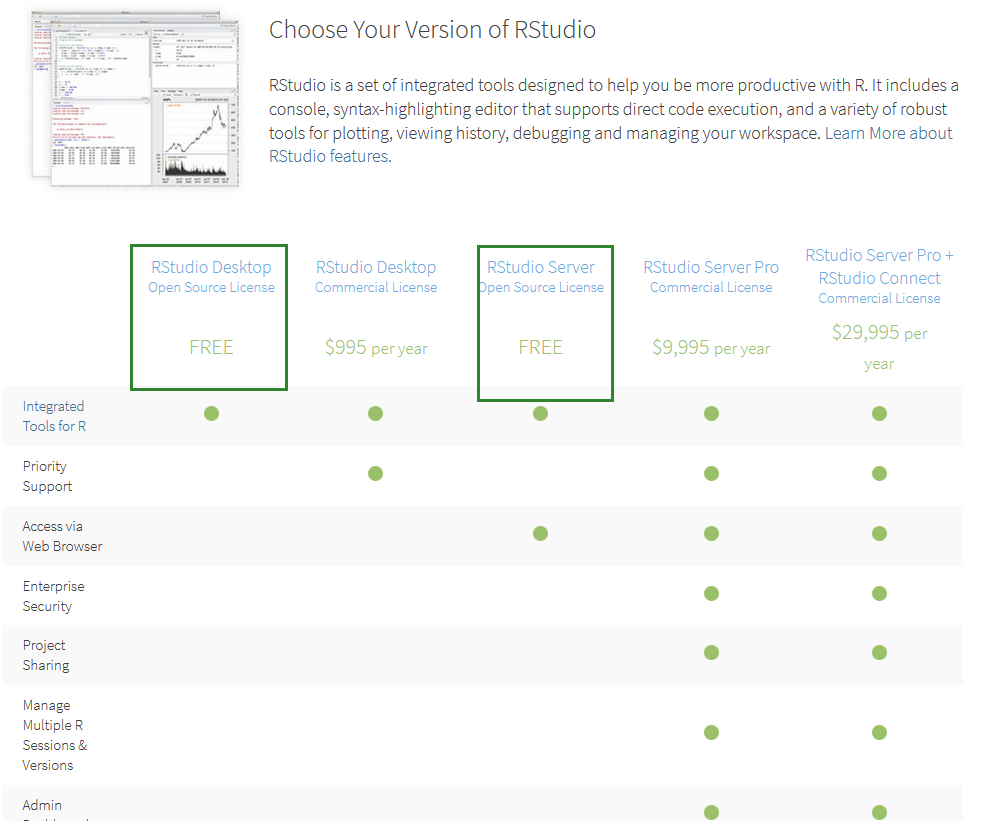
\includegraphics[width=0.95\linewidth,height=0.7\textheight,keepaspectratio]{images/Rstudio_version} \end{center}

\subsubsection{Rstudio安装}\label{rstudio}

\textbf{Linux下安装服务器版}

安装参考 \url{https://www.rstudio.com/products/rstudio/download-server/}

\begin{verbatim}
wget https://download2.rstudio.org/rstudio-server-rhel-1.0.136-x86_64.rpm
sudo yum install --nogpgcheck rstudio-server-rhel-1.0.136-x86_64.rpm
\end{verbatim}

安装完之后的检测、启动和配置

\begin{verbatim}
sudo rstudio-server verify-installation #查看是否安装正确
sudo rstudio-server start ## 启动
sudo rstudio-server status ## 查看状态
sudo rstudio-server stop ## 停止
ifconfig | grep 'inet addr' ## 查看服务端ip地址
sudo rstudio-server start ## 修改配置文件后重启
sudo rstudio-server active-sessions ## 列出活跃的sessions:
sudo rstudio-server suspend-session <pid> ## 暂停session
sudo rstudio-server suspend-all ##暂停所有session
\end{verbatim}

\begin{itemize}
\tightlist
\item
  Rstudio日志目录,方便查看错误信息:/var/log/rstudio-server/
\item
  配置文件:
\item
  /etc/rstudio/rserver.conf
\end{itemize}

\begin{Shaded}
\begin{Highlighting}[]
\KeywordTok{www-port}\NormalTok{=8787 (default)}
\KeywordTok{www-address}\NormalTok{=0.0.0.0 (default)}
\KeywordTok{rsession-ld-library-path}\NormalTok{=/opt/local/lib:/opt/local/someapp/lib}
\KeywordTok{rsession-which-r}\NormalTok{=/usr/local/bin/R}
\end{Highlighting}
\end{Shaded}

\begin{itemize}
\tightlist
\item
  /etc/rstudio/rsession.conf

  \begin{itemize}
  \tightlist
  \item
    Timeout
  \end{itemize}
\end{itemize}

\begin{verbatim}
[user]
session-timeout-minutes=30
[@powerusers]
session-timeout-minutes=0
\end{verbatim}

\textbf{Windows下安装桌面版}

下载之后
(\url{https://www.rstudio.com/products/rstudio/download2/})双击安装,需要使用\textbf{管理员权限},其它无需要注意的。

\subsubsection{Rstudio 使用}\label{rstudio-}

Windows下桌面版直接双击打开即可使用,Linux服务器版访问地址为,用户名和密码为Linux用户的用户名和密码。

\paragraph{Rstudio 界面}\label{rstudio-}

\begin{center}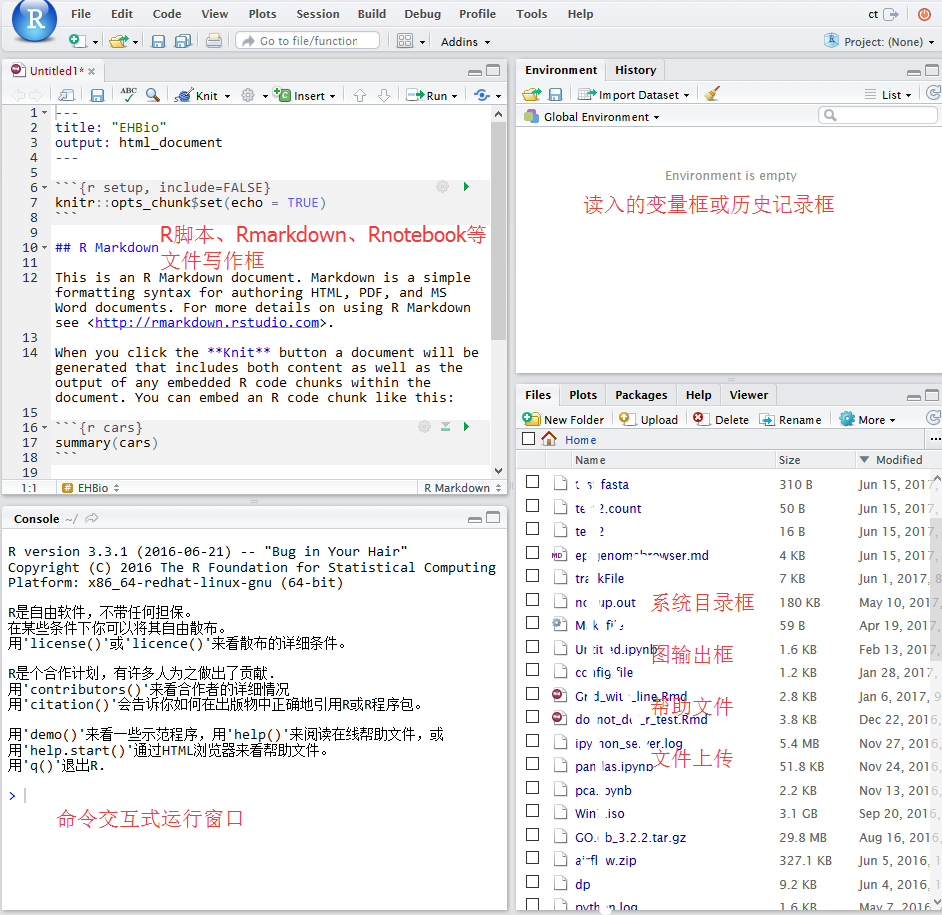
\includegraphics[width=0.95\linewidth,height=0.7\textheight,keepaspectratio]{images/Rstudio_IDE} \end{center}

\paragraph{Rstudio中新建或打开文件}\label{rstudio}

如果是桌面版,直接就可以访问``我的电脑''去打开之前写过的脚本。如果是服务器版,可直接访问服务器上写过的脚本。Rstudio右下1/4部分可以切换目录,点击more,设置工作目录。可以上传本地的脚本到对应目录打开。

\subsection{R基本语法}\label{r}

\subsubsection{获取帮助文档,查看命令或函数的使用方法、事例或适用范围}

\begin{Shaded}
\begin{Highlighting}[]
\NormalTok{>}\ErrorTok{>>}\StringTok{ }\NormalTok{?command}
\NormalTok{>}\ErrorTok{>>}\StringTok{ }\NormalTok{??command }\CommentTok{#深度搜索或模糊搜索此命令}

\NormalTok{>}\ErrorTok{>>}\StringTok{ }\KeywordTok{example}\NormalTok{(command) }\CommentTok{#得到命令的例子}

\NormalTok{>}\ErrorTok{>>}\StringTok{ }\KeywordTok{example}\NormalTok{(plot)}
\end{Highlighting}
\end{Shaded}

\subsubsection{R中的变量及其初始化}\label{r}

\begin{Shaded}
\begin{Highlighting}[]
\CommentTok{# 数字变量}
\NormalTok{a <-}\StringTok{ }\DecValTok{10}
\NormalTok{a}
\end{Highlighting}
\end{Shaded}

\begin{verbatim}
## [1] 10
\end{verbatim}

\begin{Shaded}
\begin{Highlighting}[]
\CommentTok{# 字符串变量}
\NormalTok{a <-}\StringTok{ "abc"}
\NormalTok{a}
\end{Highlighting}
\end{Shaded}

\begin{verbatim}
## [1] "abc"
\end{verbatim}

\begin{Shaded}
\begin{Highlighting}[]
\CommentTok{# 逻辑变量}
\NormalTok{a <-}\StringTok{ }\OtherTok{TRUE}
\NormalTok{a}
\end{Highlighting}
\end{Shaded}

\begin{verbatim}
## [1] TRUE
\end{verbatim}

\begin{Shaded}
\begin{Highlighting}[]
\NormalTok{b <-}\StringTok{ }\NormalTok{T}
\NormalTok{b}
\end{Highlighting}
\end{Shaded}

\begin{verbatim}
## [1] TRUE
\end{verbatim}

\begin{Shaded}
\begin{Highlighting}[]
\NormalTok{d <-}\StringTok{ }\OtherTok{FALSE}
\NormalTok{d}
\end{Highlighting}
\end{Shaded}

\begin{verbatim}
## [1] FALSE
\end{verbatim}

\begin{Shaded}
\begin{Highlighting}[]
\CommentTok{# 向量}
\NormalTok{a <-}\StringTok{ }\KeywordTok{vector}\NormalTok{(}\DataTypeTok{mode=}\StringTok{"logical"}\NormalTok{, }\DataTypeTok{length=}\DecValTok{5}\NormalTok{)}
\NormalTok{a}
\end{Highlighting}
\end{Shaded}

\begin{verbatim}
## [1] FALSE FALSE FALSE FALSE FALSE
\end{verbatim}

\begin{Shaded}
\begin{Highlighting}[]
\NormalTok{a <-}\StringTok{ }\KeywordTok{c}\NormalTok{(}\DecValTok{1}\NormalTok{,}\DecValTok{2}\NormalTok{,}\DecValTok{3}\NormalTok{,}\DecValTok{4}\NormalTok{)}
\CommentTok{# 判断一个变量是不是vector}
\KeywordTok{is.vector}\NormalTok{(a)}
\end{Highlighting}
\end{Shaded}

\begin{verbatim}
## [1] TRUE
\end{verbatim}

\begin{Shaded}
\begin{Highlighting}[]
\NormalTok{a <-}\StringTok{ }\KeywordTok{list}\NormalTok{(}\DataTypeTok{element1=}\KeywordTok{c}\NormalTok{(}\DecValTok{1}\NormalTok{,}\DecValTok{2}\NormalTok{,}\DecValTok{3}\NormalTok{,}\DecValTok{4}\NormalTok{), }\DataTypeTok{element2=}\DecValTok{1}\NormalTok{:}\DecValTok{5}\NormalTok{)}
\NormalTok{a}
\end{Highlighting}
\end{Shaded}

\begin{verbatim}
## $element1
## [1] 1 2 3 4
## 
## $element2
## [1] 1 2 3 4 5
\end{verbatim}

\begin{Shaded}
\begin{Highlighting}[]
\CommentTok{# 矩阵}
\NormalTok{a <-}\StringTok{ }\KeywordTok{matrix}\NormalTok{(}\DecValTok{1}\NormalTok{:}\DecValTok{20}\NormalTok{,}\DataTypeTok{nrow=}\DecValTok{5}\NormalTok{,}\DataTypeTok{ncol=}\DecValTok{4}\NormalTok{,}\DataTypeTok{byrow=}\NormalTok{T)}
\NormalTok{a}
\end{Highlighting}
\end{Shaded}

\begin{verbatim}
##      [,1] [,2] [,3] [,4]
## [1,]    1    2    3    4
## [2,]    5    6    7    8
## [3,]    9   10   11   12
## [4,]   13   14   15   16
## [5,]   17   18   19   20
\end{verbatim}

\begin{Shaded}
\begin{Highlighting}[]
\KeywordTok{is.matrix}\NormalTok{(a)}
\end{Highlighting}
\end{Shaded}

\begin{verbatim}
## [1] TRUE
\end{verbatim}

\begin{Shaded}
\begin{Highlighting}[]
\KeywordTok{dim}\NormalTok{(a) }\CommentTok{#查看或设置数组的维度向量}
\end{Highlighting}
\end{Shaded}

\begin{verbatim}
## [1] 5 4
\end{verbatim}

\begin{Shaded}
\begin{Highlighting}[]
\CommentTok{# 错误的用法}
\CommentTok{# dim(a) <- c(4,4)}
\end{Highlighting}
\end{Shaded}

\begin{Shaded}
\begin{Highlighting}[]
\CommentTok{# 正确的用法}
\NormalTok{a <-}\StringTok{ }\DecValTok{1}\NormalTok{:}\DecValTok{20}
\KeywordTok{dim}\NormalTok{(a) <-}\StringTok{ }\KeywordTok{c}\NormalTok{(}\DecValTok{5}\NormalTok{,}\DecValTok{4}\NormalTok{) }\CommentTok{#转换向量为矩阵}
\NormalTok{a}
\end{Highlighting}
\end{Shaded}

\begin{verbatim}
##      [,1] [,2] [,3] [,4]
## [1,]    1    6   11   16
## [2,]    2    7   12   17
## [3,]    3    8   13   18
## [4,]    4    9   14   19
## [5,]    5   10   15   20
\end{verbatim}

\begin{Shaded}
\begin{Highlighting}[]
\KeywordTok{print}\NormalTok{(}\KeywordTok{paste}\NormalTok{(}\StringTok{"矩阵a的行数"}\NormalTok{, }\KeywordTok{nrow}\NormalTok{(a)))}
\end{Highlighting}
\end{Shaded}

\begin{verbatim}
## [1] "矩阵a的行数 5"
\end{verbatim}

\begin{Shaded}
\begin{Highlighting}[]
\KeywordTok{print}\NormalTok{(}\KeywordTok{paste}\NormalTok{(}\StringTok{"矩阵a的列数"}\NormalTok{, }\KeywordTok{ncol}\NormalTok{(a)))}
\end{Highlighting}
\end{Shaded}

\begin{verbatim}
## [1] "矩阵a的列数 4"
\end{verbatim}

\begin{Shaded}
\begin{Highlighting}[]
\CommentTok{#查看或设置行列名}
\KeywordTok{rownames}\NormalTok{(a)}
\end{Highlighting}
\end{Shaded}

\begin{verbatim}
## NULL
\end{verbatim}

\begin{Shaded}
\begin{Highlighting}[]
\KeywordTok{rownames}\NormalTok{(a) <-}\StringTok{ }\KeywordTok{c}\NormalTok{(}\StringTok{'a'}\NormalTok{,}\StringTok{'b'}\NormalTok{,}\StringTok{'c'}\NormalTok{,}\StringTok{'d'}\NormalTok{,}\StringTok{'e'}\NormalTok{)}
\NormalTok{a}
\end{Highlighting}
\end{Shaded}

\begin{verbatim}
##   [,1] [,2] [,3] [,4]
## a    1    6   11   16
## b    2    7   12   17
## c    3    8   13   18
## d    4    9   14   19
## e    5   10   15   20
\end{verbatim}

\begin{Shaded}
\begin{Highlighting}[]
\CommentTok{# R中获取一系列的字母}
\NormalTok{letters[}\DecValTok{1}\NormalTok{:}\DecValTok{4}\NormalTok{]}
\end{Highlighting}
\end{Shaded}

\begin{verbatim}
## [1] "a" "b" "c" "d"
\end{verbatim}

\begin{Shaded}
\begin{Highlighting}[]
\KeywordTok{colnames}\NormalTok{(a) <-}\StringTok{ }\NormalTok{letters[}\DecValTok{1}\NormalTok{:}\DecValTok{4}\NormalTok{]}
\NormalTok{a}
\end{Highlighting}
\end{Shaded}

\begin{verbatim}
##   a  b  c  d
## a 1  6 11 16
## b 2  7 12 17
## c 3  8 13 18
## d 4  9 14 19
## e 5 10 15 20
\end{verbatim}

\subsubsection{变量类型和转换}

不同的变量类型有不同的操作方式,\texttt{is}系列和\texttt{as}系列函数用来判断变量的属性和转换变量的属性

\begin{Shaded}
\begin{Highlighting}[]
\KeywordTok{is.character}\NormalTok{(a)}
\end{Highlighting}
\end{Shaded}

\begin{verbatim}
## [1] FALSE
\end{verbatim}

\begin{Shaded}
\begin{Highlighting}[]
\KeywordTok{is.numeric}\NormalTok{(a)}
\end{Highlighting}
\end{Shaded}

\begin{verbatim}
## [1] TRUE
\end{verbatim}

\begin{Shaded}
\begin{Highlighting}[]
\KeywordTok{is.matrix}\NormalTok{(a)}
\end{Highlighting}
\end{Shaded}

\begin{verbatim}
## [1] TRUE
\end{verbatim}

\begin{Shaded}
\begin{Highlighting}[]
\KeywordTok{is.data.frame}\NormalTok{(a)}
\end{Highlighting}
\end{Shaded}

\begin{verbatim}
## [1] FALSE
\end{verbatim}

\begin{Shaded}
\begin{Highlighting}[]
\KeywordTok{is.data.frame}\NormalTok{(}\KeywordTok{as.data.frame}\NormalTok{(a))}
\end{Highlighting}
\end{Shaded}

\begin{verbatim}
## [1] TRUE
\end{verbatim}

\subsubsection{R中矩阵运算}\label{r}

\begin{Shaded}
\begin{Highlighting}[]
\CommentTok{# 获得随机的正态分布数据}
\CommentTok{# random generation for the normal distribution with mean equal to ‘mean’}
\CommentTok{# and standard deviation equal to ‘sd’.}
\KeywordTok{rnorm}\NormalTok{(}\DecValTok{10}\NormalTok{, }\DataTypeTok{mean =} \DecValTok{0}\NormalTok{, }\DataTypeTok{sd =} \DecValTok{1}\NormalTok{) }\CommentTok{# 正态分布的随机数}
\end{Highlighting}
\end{Shaded}

\begin{verbatim}
##  [1] -1.7623698  0.1703914 -1.0272638 -1.2723234 -0.9341441  2.2230742
##  [7] -0.3978386  1.6669337 -1.0560411 -2.8457878
\end{verbatim}

\begin{Shaded}
\begin{Highlighting}[]
\CommentTok{# 获得随机的均匀分布的数据}
\CommentTok{# random generation for the uniform distribution with mean equal to ‘mean’}
\CommentTok{# and standard deviation equal to ‘sd’.}
\KeywordTok{runif}\NormalTok{(}\DecValTok{10}\NormalTok{, }\DataTypeTok{min =} \DecValTok{0}\NormalTok{, }\DataTypeTok{max =} \DecValTok{1}\NormalTok{) }\CommentTok{# 平均分布的随机数}
\end{Highlighting}
\end{Shaded}

\begin{verbatim}
##  [1] 0.1204988 0.2521150 0.9239175 0.7009465 0.8067070 0.4582831 0.9140327
##  [8] 0.4635908 0.6317504 0.3384500
\end{verbatim}

\begin{Shaded}
\begin{Highlighting}[]
\KeywordTok{rep}\NormalTok{(}\DecValTok{1}\NormalTok{,}\DecValTok{5}\NormalTok{) }\CommentTok{# 把1重复5次}
\end{Highlighting}
\end{Shaded}

\begin{verbatim}
## [1] 1 1 1 1 1
\end{verbatim}

\begin{Shaded}
\begin{Highlighting}[]
\KeywordTok{scale}\NormalTok{(}\DecValTok{1}\NormalTok{:}\DecValTok{5}\NormalTok{) }\CommentTok{# 标准化数据}
\end{Highlighting}
\end{Shaded}

\begin{verbatim}
##            [,1]
## [1,] -1.2649111
## [2,] -0.6324555
## [3,]  0.0000000
## [4,]  0.6324555
## [5,]  1.2649111
## attr(,"scaled:center")
## [1] 3
## attr(,"scaled:scale")
## [1] 1.581139
\end{verbatim}

\texttt{scale}默认操作对等于

\begin{Shaded}
\begin{Highlighting}[]
\CommentTok{# 标准化数据}
\NormalTok{a <-}\StringTok{ }\DecValTok{1}\NormalTok{:}\DecValTok{5}
\NormalTok{(a -}\StringTok{ }\KeywordTok{mean}\NormalTok{(a)) /}\StringTok{ }\KeywordTok{sd}\NormalTok{(a)}
\end{Highlighting}
\end{Shaded}

\begin{verbatim}
## [1] -1.2649111 -0.6324555  0.0000000  0.6324555  1.2649111
\end{verbatim}

\begin{Shaded}
\begin{Highlighting}[]
\NormalTok{a <-}\StringTok{ }\KeywordTok{c}\NormalTok{(}\KeywordTok{rnorm}\NormalTok{(}\DecValTok{5}\NormalTok{), }\KeywordTok{rnorm}\NormalTok{(}\DecValTok{5}\NormalTok{,}\DecValTok{1}\NormalTok{), }\KeywordTok{runif}\NormalTok{(}\DecValTok{5}\NormalTok{), }\KeywordTok{runif}\NormalTok{(}\DecValTok{5}\NormalTok{,-}\DecValTok{1}\NormalTok{,}\DecValTok{1}\NormalTok{), }\DecValTok{1}\NormalTok{:}\DecValTok{5}\NormalTok{, }\KeywordTok{rep}\NormalTok{(}\DecValTok{0}\NormalTok{,}\DecValTok{5}\NormalTok{), }\KeywordTok{c}\NormalTok{(}\DecValTok{2}\NormalTok{,}\DecValTok{10}\NormalTok{,}\DecValTok{11}\NormalTok{,}\DecValTok{13}\NormalTok{,}\DecValTok{4}\NormalTok{), }
        \KeywordTok{scale}\NormalTok{(}\DecValTok{1}\NormalTok{:}\DecValTok{5}\NormalTok{)[}\DecValTok{1}\NormalTok{:}\DecValTok{5}\NormalTok{])}
\NormalTok{a}
\end{Highlighting}
\end{Shaded}

\begin{verbatim}
##  [1]  0.571515883 -0.786827497 -0.069386297 -0.366760489 -2.336466642
##  [6] -0.256031715  0.976938913  2.239830880  1.307826807  1.689656291
## [11]  0.005828207  0.908370379  0.220653976  0.415340775  0.237234787
## [16] -0.996525097  0.179710705 -0.499995762 -0.680745059 -0.838659695
## [21]  1.000000000  2.000000000  3.000000000  4.000000000  5.000000000
## [26]  0.000000000  0.000000000  0.000000000  0.000000000  0.000000000
## [31]  2.000000000 10.000000000 11.000000000 13.000000000  4.000000000
## [36] -1.264911064 -0.632455532  0.000000000  0.632455532  1.264911064
\end{verbatim}

\begin{Shaded}
\begin{Highlighting}[]
\CommentTok{# ncol=5 5列}
\CommentTok{# byrow=T: 先填充行}
\NormalTok{a <-}\StringTok{ }\KeywordTok{matrix}\NormalTok{(a, }\DataTypeTok{ncol=}\DecValTok{5}\NormalTok{, }\DataTypeTok{byrow=}\NormalTok{T)}
\NormalTok{a}
\end{Highlighting}
\end{Shaded}

\begin{verbatim}
##              [,1]       [,2]       [,3]       [,4]       [,5]
## [1,]  0.571515883 -0.7868275 -0.0693863 -0.3667605 -2.3364666
## [2,] -0.256031715  0.9769389  2.2398309  1.3078268  1.6896563
## [3,]  0.005828207  0.9083704  0.2206540  0.4153408  0.2372348
## [4,] -0.996525097  0.1797107 -0.4999958 -0.6807451 -0.8386597
## [5,]  1.000000000  2.0000000  3.0000000  4.0000000  5.0000000
## [6,]  0.000000000  0.0000000  0.0000000  0.0000000  0.0000000
## [7,]  2.000000000 10.0000000 11.0000000 13.0000000  4.0000000
## [8,] -1.264911064 -0.6324555  0.0000000  0.6324555  1.2649111
\end{verbatim}

\begin{Shaded}
\begin{Highlighting}[]
\CommentTok{# 按行加和}
\KeywordTok{rowSums}\NormalTok{(a)}
\end{Highlighting}
\end{Shaded}

\begin{verbatim}
## [1] -2.987925  5.958221  1.787428 -2.836215 15.000000  0.000000 40.000000
## [8]  0.000000
\end{verbatim}

\begin{Shaded}
\begin{Highlighting}[]
\CommentTok{# 注意检查括号的配对}
\CommentTok{#a <- a[rowSums(abs(a)!=0,]}
\CommentTok{#错误: 意外的']' in "a <- a[rowSums(abs(a)!=0,]"}

\CommentTok{# 去除全部为0的行}
\NormalTok{a <-}\StringTok{ }\NormalTok{a[}\KeywordTok{rowSums}\NormalTok{(}\KeywordTok{abs}\NormalTok{(a))!=}\DecValTok{0}\NormalTok{,]}

\CommentTok{# 另外一种方式去除全部为0的行}
\CommentTok{#a[rowSums(a==0)<ncol(a),]}

\NormalTok{a}
\end{Highlighting}
\end{Shaded}

\begin{verbatim}
##              [,1]       [,2]       [,3]       [,4]       [,5]
## [1,]  0.571515883 -0.7868275 -0.0693863 -0.3667605 -2.3364666
## [2,] -0.256031715  0.9769389  2.2398309  1.3078268  1.6896563
## [3,]  0.005828207  0.9083704  0.2206540  0.4153408  0.2372348
## [4,] -0.996525097  0.1797107 -0.4999958 -0.6807451 -0.8386597
## [5,]  1.000000000  2.0000000  3.0000000  4.0000000  5.0000000
## [6,]  2.000000000 10.0000000 11.0000000 13.0000000  4.0000000
## [7,] -1.264911064 -0.6324555  0.0000000  0.6324555  1.2649111
\end{verbatim}

矩阵运算,R默认针对整个数据进行常见运算

\begin{Shaded}
\begin{Highlighting}[]
\CommentTok{#所有值都乘以2}
\NormalTok{a *}\StringTok{ }\DecValTok{2}
\end{Highlighting}
\end{Shaded}

\begin{verbatim}
##             [,1]       [,2]       [,3]       [,4]       [,5]
## [1,]  1.14303177 -1.5736550 -0.1387726 -0.7335210 -4.6729333
## [2,] -0.51206343  1.9538778  4.4796618  2.6156536  3.3793126
## [3,]  0.01165641  1.8167408  0.4413080  0.8306815  0.4744696
## [4,] -1.99305019  0.3594214 -0.9999915 -1.3614901 -1.6773194
## [5,]  2.00000000  4.0000000  6.0000000  8.0000000 10.0000000
## [6,]  4.00000000 20.0000000 22.0000000 26.0000000  8.0000000
## [7,] -2.52982213 -1.2649111  0.0000000  1.2649111  2.5298221
\end{verbatim}

\begin{Shaded}
\begin{Highlighting}[]
\CommentTok{# 所有值取绝对值,再取对数 (取对数前一般加一个数避免对0或负值取对数)}
\KeywordTok{log2}\NormalTok{(}\KeywordTok{abs}\NormalTok{(a)+}\DecValTok{1}\NormalTok{)}
\end{Highlighting}
\end{Shaded}

\begin{verbatim}
##             [,1]      [,2]      [,3]      [,4]      [,5]
## [1,] 0.652156854 0.8374004 0.0967831 0.4507604 1.7383211
## [2,] 0.328872893 0.9832683 1.6959185 1.2065350 1.4274218
## [3,] 0.008383917 0.9323412 0.2876543 0.5011495 0.3071193
## [4,] 0.997491207 0.2384331 0.5849584 0.7491009 0.8786545
## [5,] 1.000000000 1.5849625 2.0000000 2.3219281 2.5849625
## [6,] 1.584962501 3.4594316 3.5849625 3.8073549 2.3219281
## [7,] 1.179454401 0.7070437 0.0000000 0.7070437 1.1794544
\end{verbatim}

\begin{Shaded}
\begin{Highlighting}[]
\CommentTok{# 取出最大值、最小值、行数、列数}
\KeywordTok{max}\NormalTok{(a)}
\end{Highlighting}
\end{Shaded}

\begin{verbatim}
## [1] 13
\end{verbatim}

\begin{Shaded}
\begin{Highlighting}[]
\KeywordTok{min}\NormalTok{(a)}
\end{Highlighting}
\end{Shaded}

\begin{verbatim}
## [1] -2.336467
\end{verbatim}

\begin{Shaded}
\begin{Highlighting}[]
\KeywordTok{nrow}\NormalTok{(a)}
\end{Highlighting}
\end{Shaded}

\begin{verbatim}
## [1] 7
\end{verbatim}

\begin{Shaded}
\begin{Highlighting}[]
\KeywordTok{ncol}\NormalTok{(a)}
\end{Highlighting}
\end{Shaded}

\begin{verbatim}
## [1] 5
\end{verbatim}

\begin{Shaded}
\begin{Highlighting}[]
\CommentTok{#增加一列或一行}
\CommentTok{#cbind: column bind}
\KeywordTok{cbind}\NormalTok{(a, }\DecValTok{1}\NormalTok{:}\DecValTok{7}\NormalTok{)}
\end{Highlighting}
\end{Shaded}

\begin{verbatim}
##              [,1]       [,2]       [,3]       [,4]       [,5] [,6]
## [1,]  0.571515883 -0.7868275 -0.0693863 -0.3667605 -2.3364666    1
## [2,] -0.256031715  0.9769389  2.2398309  1.3078268  1.6896563    2
## [3,]  0.005828207  0.9083704  0.2206540  0.4153408  0.2372348    3
## [4,] -0.996525097  0.1797107 -0.4999958 -0.6807451 -0.8386597    4
## [5,]  1.000000000  2.0000000  3.0000000  4.0000000  5.0000000    5
## [6,]  2.000000000 10.0000000 11.0000000 13.0000000  4.0000000    6
## [7,] -1.264911064 -0.6324555  0.0000000  0.6324555  1.2649111    7
\end{verbatim}

\begin{Shaded}
\begin{Highlighting}[]
\CommentTok{# rbind: row bind}
\KeywordTok{rbind}\NormalTok{(a,}\DecValTok{1}\NormalTok{:}\DecValTok{5}\NormalTok{)}
\end{Highlighting}
\end{Shaded}

\begin{verbatim}
##              [,1]       [,2]       [,3]       [,4]       [,5]
## [1,]  0.571515883 -0.7868275 -0.0693863 -0.3667605 -2.3364666
## [2,] -0.256031715  0.9769389  2.2398309  1.3078268  1.6896563
## [3,]  0.005828207  0.9083704  0.2206540  0.4153408  0.2372348
## [4,] -0.996525097  0.1797107 -0.4999958 -0.6807451 -0.8386597
## [5,]  1.000000000  2.0000000  3.0000000  4.0000000  5.0000000
## [6,]  2.000000000 10.0000000 11.0000000 13.0000000  4.0000000
## [7,] -1.264911064 -0.6324555  0.0000000  0.6324555  1.2649111
## [8,]  1.000000000  2.0000000  3.0000000  4.0000000  5.0000000
\end{verbatim}

\begin{Shaded}
\begin{Highlighting}[]
\CommentTok{# 计算每一行的var (方差)}
\CommentTok{# apply表示对数据(第一个参数)的每一行 (第二个参数赋值为1) 或每一列 (2)操作}
\CommentTok{#      最后返回一个列表}
\KeywordTok{apply}\NormalTok{(a,}\DecValTok{1}\NormalTok{,var)}
\end{Highlighting}
\end{Shaded}

\begin{verbatim}
## [1]  1.1896482  0.8755184  0.1159168  0.2083237  2.5000000 22.5000000
## [7]  1.0000000
\end{verbatim}

\begin{Shaded}
\begin{Highlighting}[]
\CommentTok{# 计算每一行的mad (中值绝对偏差)}
\CommentTok{# 一般认为比方差的鲁棒性更强,更少受异常值的影响,更能反映数据间的差异)}
\CommentTok{# 函数中的第二个参数 1 表示安行操作}
\KeywordTok{apply}\NormalTok{(a,}\DecValTok{1}\NormalTok{,mad)}
\end{Highlighting}
\end{Shaded}

\begin{verbatim}
## [1] 0.6227913 0.5661004 0.2640599 0.2679789 1.4826000 4.4478000 0.9376786
\end{verbatim}

\begin{Shaded}
\begin{Highlighting}[]
\CommentTok{# 计算每一列的平均值}
\KeywordTok{apply}\NormalTok{(a,}\DecValTok{2}\NormalTok{,mean)}
\end{Highlighting}
\end{Shaded}

\begin{verbatim}
## [1] 0.1514109 1.8065339 2.2701575 2.6154454 1.2880965
\end{verbatim}

\begin{Shaded}
\begin{Highlighting}[]
\CommentTok{# 取出中值绝对偏差大于0.5的行}
\NormalTok{b =}\StringTok{ }\NormalTok{a[}\KeywordTok{apply}\NormalTok{(a,}\DecValTok{1}\NormalTok{,mad)>}\FloatTok{0.5}\NormalTok{,]}
\NormalTok{b}
\end{Highlighting}
\end{Shaded}

\begin{verbatim}
##            [,1]       [,2]       [,3]       [,4]      [,5]
## [1,]  0.5715159 -0.7868275 -0.0693863 -0.3667605 -2.336467
## [2,] -0.2560317  0.9769389  2.2398309  1.3078268  1.689656
## [3,]  1.0000000  2.0000000  3.0000000  4.0000000  5.000000
## [4,]  2.0000000 10.0000000 11.0000000 13.0000000  4.000000
## [5,] -1.2649111 -0.6324555  0.0000000  0.6324555  1.264911
\end{verbatim}

\begin{Shaded}
\begin{Highlighting}[]
\CommentTok{# 输出 1 4 2 3 5}
\CommentTok{# 解释:原列表第一个元素显示在第一位}
\CommentTok{#       原列表第四个元素显示在第二位}
\CommentTok{#       原列表第二个元素显示在第三位}
\KeywordTok{order}\NormalTok{(}\KeywordTok{c}\NormalTok{(}\DecValTok{1}\NormalTok{,}\DecValTok{3}\NormalTok{,}\DecValTok{4}\NormalTok{,}\DecValTok{2}\NormalTok{,}\DecValTok{5}\NormalTok{))}
\end{Highlighting}
\end{Shaded}

\begin{verbatim}
## [1] 1 4 2 3 5
\end{verbatim}

\begin{Shaded}
\begin{Highlighting}[]
\CommentTok{# 产生新的顺序}
\CommentTok{# }
\KeywordTok{order}\NormalTok{(}\KeywordTok{apply}\NormalTok{(b,}\DecValTok{1}\NormalTok{,mad), }\DataTypeTok{decreasing=}\NormalTok{T)}
\end{Highlighting}
\end{Shaded}

\begin{verbatim}
## [1] 4 3 5 1 2
\end{verbatim}

\begin{Shaded}
\begin{Highlighting}[]
\CommentTok{# 矩阵按照mad的大小降序排列}
\NormalTok{c =}\StringTok{ }\NormalTok{b[}\KeywordTok{order}\NormalTok{(}\KeywordTok{apply}\NormalTok{(b,}\DecValTok{1}\NormalTok{,mad), }\DataTypeTok{decreasing=}\NormalTok{T),]}
\NormalTok{c}
\end{Highlighting}
\end{Shaded}

\begin{verbatim}
##            [,1]       [,2]       [,3]       [,4]      [,5]
## [1,]  2.0000000 10.0000000 11.0000000 13.0000000  4.000000
## [2,]  1.0000000  2.0000000  3.0000000  4.0000000  5.000000
## [3,] -1.2649111 -0.6324555  0.0000000  0.6324555  1.264911
## [4,]  0.5715159 -0.7868275 -0.0693863 -0.3667605 -2.336467
## [5,] -0.2560317  0.9769389  2.2398309  1.3078268  1.689656
\end{verbatim}

\begin{Shaded}
\begin{Highlighting}[]
\KeywordTok{rownames}\NormalTok{(c) <-}\StringTok{ }\KeywordTok{paste}\NormalTok{(}\StringTok{'Gene'}\NormalTok{, letters[}\DecValTok{1}\NormalTok{:}\KeywordTok{nrow}\NormalTok{(c)], }\DataTypeTok{sep=}\StringTok{"_"}\NormalTok{)}
\KeywordTok{colnames}\NormalTok{(c) <-}\StringTok{ }\KeywordTok{toupper}\NormalTok{(letters[}\DecValTok{1}\NormalTok{:}\KeywordTok{ncol}\NormalTok{(c)])}
\NormalTok{c}
\end{Highlighting}
\end{Shaded}

\begin{verbatim}
##                 A          B          C          D         E
## Gene_a  2.0000000 10.0000000 11.0000000 13.0000000  4.000000
## Gene_b  1.0000000  2.0000000  3.0000000  4.0000000  5.000000
## Gene_c -1.2649111 -0.6324555  0.0000000  0.6324555  1.264911
## Gene_d  0.5715159 -0.7868275 -0.0693863 -0.3667605 -2.336467
## Gene_e -0.2560317  0.9769389  2.2398309  1.3078268  1.689656
\end{verbatim}

\begin{Shaded}
\begin{Highlighting}[]
\CommentTok{# 矩阵转置}
\NormalTok{expr =}\StringTok{ }\KeywordTok{t}\NormalTok{(c)}
\NormalTok{expr}
\end{Highlighting}
\end{Shaded}

\begin{verbatim}
##   Gene_a Gene_b     Gene_c     Gene_d     Gene_e
## A      2      1 -1.2649111  0.5715159 -0.2560317
## B     10      2 -0.6324555 -0.7868275  0.9769389
## C     11      3  0.0000000 -0.0693863  2.2398309
## D     13      4  0.6324555 -0.3667605  1.3078268
## E      4      5  1.2649111 -2.3364666  1.6896563
\end{verbatim}

\begin{Shaded}
\begin{Highlighting}[]
\CommentTok{# 矩阵值的替换}
\NormalTok{expr2 =}\StringTok{ }\NormalTok{expr}
\NormalTok{expr2[expr2<}\DecValTok{0}\NormalTok{] =}\StringTok{ }\DecValTok{0}
\NormalTok{expr2}
\end{Highlighting}
\end{Shaded}

\begin{verbatim}
##   Gene_a Gene_b    Gene_c    Gene_d    Gene_e
## A      2      1 0.0000000 0.5715159 0.0000000
## B     10      2 0.0000000 0.0000000 0.9769389
## C     11      3 0.0000000 0.0000000 2.2398309
## D     13      4 0.6324555 0.0000000 1.3078268
## E      4      5 1.2649111 0.0000000 1.6896563
\end{verbatim}

\begin{Shaded}
\begin{Highlighting}[]
\CommentTok{# 矩阵中只针对某一列替换}
\CommentTok{# expr2是个矩阵不是数据框,不能使用列名字索引}
\CommentTok{# expr2[expr2$Gene_b<1, "Gene_b"] <- 1}
\end{Highlighting}
\end{Shaded}

\begin{Shaded}
\begin{Highlighting}[]
\CommentTok{# str是一个最为常用、好用的查看变量信息的工具,尤其是对特别复杂的变量,}
\CommentTok{#    可以看清其层级结构,便于提取数据}
\KeywordTok{str}\NormalTok{(expr2)}
\end{Highlighting}
\end{Shaded}

\begin{verbatim}
##  num [1:5, 1:5] 2 10 11 13 4 1 2 3 4 5 ...
##  - attr(*, "dimnames")=List of 2
##   ..$ : chr [1:5] "A" "B" "C" "D" ...
##   ..$ : chr [1:5] "Gene_a" "Gene_b" "Gene_c" "Gene_d" ...
\end{verbatim}

\begin{Shaded}
\begin{Highlighting}[]
\CommentTok{# 转换为数据框,再进行相应的操作}
\NormalTok{expr2 <-}\StringTok{ }\KeywordTok{as.data.frame}\NormalTok{(expr2)}
\KeywordTok{str}\NormalTok{(expr2)}
\end{Highlighting}
\end{Shaded}

\begin{verbatim}
## 'data.frame':    5 obs. of  5 variables:
##  $ Gene_a: num  2 10 11 13 4
##  $ Gene_b: num  1 2 3 4 5
##  $ Gene_c: num  0 0 0 0.632 1.265
##  $ Gene_d: num  0.572 0 0 0 0
##  $ Gene_e: num  0 0.977 2.24 1.308 1.69
\end{verbatim}

\begin{Shaded}
\begin{Highlighting}[]
\NormalTok{expr2[expr2$Gene_b<}\DecValTok{1}\NormalTok{, }\StringTok{"Gene_b"}\NormalTok{] <-}\StringTok{ }\DecValTok{1}
\NormalTok{expr2}
\end{Highlighting}
\end{Shaded}

\begin{verbatim}
##   Gene_a Gene_b    Gene_c    Gene_d    Gene_e
## A      2      1 0.0000000 0.5715159 0.0000000
## B     10      2 0.0000000 0.0000000 0.9769389
## C     11      3 0.0000000 0.0000000 2.2398309
## D     13      4 0.6324555 0.0000000 1.3078268
## E      4      5 1.2649111 0.0000000 1.6896563
\end{verbatim}

\subsubsection{R中矩阵筛选合并}\label{r}

\begin{Shaded}
\begin{Highlighting}[]
\CommentTok{# 读入样品信息}
\NormalTok{sampleInfo =}\StringTok{ "Samp;Group;Genotype}
\StringTok{A;Control;WT}
\StringTok{B;Control;WT}
\StringTok{D;Treatment;Mutant}
\StringTok{C;Treatment;Mutant}
\StringTok{E;Treatment;WT}
\StringTok{F;Treatment;WT"}

\NormalTok{phenoData =}\StringTok{ }\KeywordTok{read.table}\NormalTok{(}\DataTypeTok{text=}\NormalTok{sampleInfo,}\DataTypeTok{sep=}\StringTok{";"}\NormalTok{, }\DataTypeTok{header=}\NormalTok{T, }\DataTypeTok{row.names=}\DecValTok{1}\NormalTok{, }\DataTypeTok{quote=}\StringTok{""}\NormalTok{)}
\NormalTok{phenoData}
\end{Highlighting}
\end{Shaded}

\begin{verbatim}
##       Group Genotype
## A   Control       WT
## B   Control       WT
## D Treatment   Mutant
## C Treatment   Mutant
## E Treatment       WT
## F Treatment       WT
\end{verbatim}

\begin{Shaded}
\begin{Highlighting}[]
\CommentTok{# 把样品信息按照基因表达矩阵中的样品信息排序,并只保留有基因表达信息的样品}
\CommentTok{# ‘%in%’ is a more intuitive interface as a binary operator, which}
\CommentTok{#     returns a logical vector indicating if there is a match or not for}
\CommentTok{#     its left operand.}
     
\NormalTok{phenoData =}\StringTok{ }\NormalTok{phenoData[}\KeywordTok{rownames}\NormalTok{(phenoData) %in%}\StringTok{ }\KeywordTok{rownames}\NormalTok{(expr),]}
\NormalTok{phenoData}
\end{Highlighting}
\end{Shaded}

\begin{verbatim}
##       Group Genotype
## A   Control       WT
## B   Control       WT
## D Treatment   Mutant
## C Treatment   Mutant
## E Treatment       WT
\end{verbatim}

\begin{Shaded}
\begin{Highlighting}[]
\CommentTok{# 合并矩阵}
\CommentTok{# by=0 表示按照行的名字排序}
\CommentTok{# by=columnname 表示按照共有的某一列合并}
\CommentTok{# 合并后多出了新的一列Row.names}
\NormalTok{merge_data =}\StringTok{ }\KeywordTok{merge}\NormalTok{(expr, phenoData, }\DataTypeTok{by=}\DecValTok{0}\NormalTok{, }\DataTypeTok{all.x=}\NormalTok{T)}
\NormalTok{merge_data}
\end{Highlighting}
\end{Shaded}

\begin{verbatim}
##   Row.names Gene_a Gene_b     Gene_c     Gene_d     Gene_e     Group
## 1         A      2      1 -1.2649111  0.5715159 -0.2560317   Control
## 2         B     10      2 -0.6324555 -0.7868275  0.9769389   Control
## 3         C     11      3  0.0000000 -0.0693863  2.2398309 Treatment
## 4         D     13      4  0.6324555 -0.3667605  1.3078268 Treatment
## 5         E      4      5  1.2649111 -2.3364666  1.6896563 Treatment
##   Genotype
## 1       WT
## 2       WT
## 3   Mutant
## 4   Mutant
## 5       WT
\end{verbatim}

\begin{Shaded}
\begin{Highlighting}[]
\KeywordTok{rownames}\NormalTok{(merge_data) <-}\StringTok{ }\NormalTok{merge_data$Row.names}
\NormalTok{merge_data}
\end{Highlighting}
\end{Shaded}

\begin{verbatim}
##   Row.names Gene_a Gene_b     Gene_c     Gene_d     Gene_e     Group
## A         A      2      1 -1.2649111  0.5715159 -0.2560317   Control
## B         B     10      2 -0.6324555 -0.7868275  0.9769389   Control
## C         C     11      3  0.0000000 -0.0693863  2.2398309 Treatment
## D         D     13      4  0.6324555 -0.3667605  1.3078268 Treatment
## E         E      4      5  1.2649111 -2.3364666  1.6896563 Treatment
##   Genotype
## A       WT
## B       WT
## C   Mutant
## D   Mutant
## E       WT
\end{verbatim}

\begin{Shaded}
\begin{Highlighting}[]
\CommentTok{# 去除一列;-1表示去除第一列}
\NormalTok{merge_data =}\StringTok{ }\NormalTok{merge_data[,-}\DecValTok{1}\NormalTok{]}
\NormalTok{merge_data}
\end{Highlighting}
\end{Shaded}

\begin{verbatim}
##   Gene_a Gene_b     Gene_c     Gene_d     Gene_e     Group Genotype
## A      2      1 -1.2649111  0.5715159 -0.2560317   Control       WT
## B     10      2 -0.6324555 -0.7868275  0.9769389   Control       WT
## C     11      3  0.0000000 -0.0693863  2.2398309 Treatment   Mutant
## D     13      4  0.6324555 -0.3667605  1.3078268 Treatment   Mutant
## E      4      5  1.2649111 -2.3364666  1.6896563 Treatment       WT
\end{verbatim}

\begin{Shaded}
\begin{Highlighting}[]
\CommentTok{# 提取出所有的数值列}
\NormalTok{merge_data[}\KeywordTok{sapply}\NormalTok{(merge_data, is.numeric)]}
\end{Highlighting}
\end{Shaded}

\begin{verbatim}
##   Gene_a Gene_b     Gene_c     Gene_d     Gene_e
## A      2      1 -1.2649111  0.5715159 -0.2560317
## B     10      2 -0.6324555 -0.7868275  0.9769389
## C     11      3  0.0000000 -0.0693863  2.2398309
## D     13      4  0.6324555 -0.3667605  1.3078268
## E      4      5  1.2649111 -2.3364666  1.6896563
\end{verbatim}

\subsubsection{\texorpdfstring{\texttt{str}的应用}{str的应用}}\label{str}

\texttt{str}: Compactly display the internal \emph{str}ucture of an R
object, a diagnostic function and an alternative to `summary (and to
some extent, 'dput'). Ideally, only one line for each `basic' structure
is displayed. It is especially well suited to compactly display the
(abbreviated) contents of (possibly nested) lists. The idea is to give
reasonable output for \emph{any} R object. It calls `args' for
(non-primitive) function objects.

\texttt{str}用来告诉结果的构成方式,对于不少Bioconductor的包,或者复杂的R函数的输出,都是一堆列表的嵌套,\texttt{str(complex\_result)}会输出每个列表的名字,方便提取对应的信息。

\begin{Shaded}
\begin{Highlighting}[]
\CommentTok{# str的一个应用例子}
\KeywordTok{str}\NormalTok{(}\KeywordTok{list}\NormalTok{(}\DataTypeTok{a =} \StringTok{"A"}\NormalTok{, }\DataTypeTok{L =} \KeywordTok{as.list}\NormalTok{(}\DecValTok{1}\NormalTok{:}\DecValTok{100}\NormalTok{)), }\DataTypeTok{list.len =} \DecValTok{9}\NormalTok{)}
\end{Highlighting}
\end{Shaded}

\begin{verbatim}
## List of 2
##  $ a: chr "A"
##  $ L:List of 100
##   ..$ : int 1
##   ..$ : int 2
##   ..$ : int 3
##   ..$ : int 4
##   ..$ : int 5
##   ..$ : int 6
##   ..$ : int 7
##   ..$ : int 8
##   ..$ : int 9
##   .. [list output truncated]
\end{verbatim}

利用\texttt{str}查看\texttt{pca}的结果,具体的\texttt{PCA}应用查看
\url{http://mp.weixin.qq.com/s/sRElBMkyR9rGa4TQp9KjNQ}。

\begin{Shaded}
\begin{Highlighting}[]
\NormalTok{pca_result <-}\StringTok{ }\KeywordTok{prcomp}\NormalTok{(expr)}
\NormalTok{pca_result}
\end{Highlighting}
\end{Shaded}

\begin{verbatim}
## Standard deviations (1, .., p=5):
## [1] 4.799777e+00 2.119814e+00 5.265774e-01 5.063709e-01 5.680469e-17
## 
## Rotation (n x k) = (5 x 5):
##               PC1        PC2         PC3         PC4           PC5
## Gene_a 0.98679759 -0.1185723  0.08127263 -0.07460493  0.000000e+00
## Gene_b 0.09365872  0.7063884 -0.36055227 -0.27664287  5.345225e-01
## Gene_c 0.05923498  0.4467592 -0.22803328 -0.17496431 -8.451543e-01
## Gene_d 0.01529138 -0.4638203 -0.88544023 -0.02515012  1.186551e-15
## Gene_e 0.11711516  0.2687620 -0.16550907  0.94162508 -1.332268e-15
\end{verbatim}

\begin{Shaded}
\begin{Highlighting}[]
\KeywordTok{str}\NormalTok{(pca_result)}
\end{Highlighting}
\end{Shaded}

\begin{verbatim}
## List of 5
##  $ sdev    : num [1:5] 4.80 2.12 5.27e-01 5.06e-01 5.68e-17
##  $ rotation: num [1:5, 1:5] 0.9868 0.0937 0.0592 0.0153 0.1171 ...
##   ..- attr(*, "dimnames")=List of 2
##   .. ..$ : chr [1:5] "Gene_a" "Gene_b" "Gene_c" "Gene_d" ...
##   .. ..$ : chr [1:5] "PC1" "PC2" "PC3" "PC4" ...
##  $ center  : Named num [1:5] 8 3 0 -0.598 1.192
##   ..- attr(*, "names")= chr [1:5] "Gene_a" "Gene_b" "Gene_c" "Gene_d" ...
##  $ scale   : logi FALSE
##  $ x       : num [1:5, 1:5] -6.33 1.81 3.09 5.08 -3.65 ...
##   ..- attr(*, "dimnames")=List of 2
##   .. ..$ : chr [1:5] "A" "B" "C" "D" ...
##   .. ..$ : chr [1:5] "PC1" "PC2" "PC3" "PC4" ...
##  - attr(*, "class")= chr "prcomp"
\end{verbatim}

\begin{Shaded}
\begin{Highlighting}[]
\CommentTok{# 取出每个主成分解释的差异}
\NormalTok{pca_result$sdev}
\end{Highlighting}
\end{Shaded}

\begin{verbatim}
## [1] 4.799777e+00 2.119814e+00 5.265774e-01 5.063709e-01 5.680469e-17
\end{verbatim}

\subsubsection{R的包管理}\label{r}

什么时候需要安装包

\begin{Shaded}
\begin{Highlighting}[]
\KeywordTok{library}\NormalTok{(}\StringTok{'unExistedPackage'}\NormalTok{)}
\NormalTok{Error in }\KeywordTok{library}\NormalTok{(}\StringTok{"unExistedPackage"}\NormalTok{) :}\StringTok{ }
\StringTok{  }\NormalTok{不存在叫‘unExistedPackage’这个名字的程辑包}
\end{Highlighting}
\end{Shaded}

如何安装R包

\begin{verbatim}
install.packages("package_name")
# 指定安装来源
install.packages("package_name", repo="http://cran.us.r-project.org")

# 安装Bioconductor的包
source('https://bioconductor.org/biocLite.R')
biocLite('BiocInstaller')
biocLite(c("RUVSeq","pcaMethods"))

# 安装Github的R包
install.packages("devtools")
devtools::install_github("JustinaZ/pcaReduce")

# 手动安装, 首先下载包的源文件(压缩版就可),然后在终端运行下面的命令。
ct@ehbio:~$ R CMD INSTALL package.tar.gz

# 移除包
remove.packages("package_name")

# 查看所有安装的包
library()

# 查看特定安装包的版本
installed.packages()[c("ggplot2"), c("Package", "Version")]

#  Package  Version 
# "DESeq2" "1.14.1" 

# 查看默认安装包的位置
.libPaths()

# 查看已加载的包
.packages()

# 调用安装的包
library(package_name)
\end{verbatim}

自动安装包

\begin{Shaded}
\begin{Highlighting}[]
\NormalTok{usePackage <-}\StringTok{ }\NormalTok{function(p) \{}
    \NormalTok{if (!}\KeywordTok{is.element}\NormalTok{(p, }\KeywordTok{installed.packages}\NormalTok{()[,}\DecValTok{1}\NormalTok{])) \{}
        \KeywordTok{install.packages}\NormalTok{(p, }\DataTypeTok{dep =} \OtherTok{TRUE}\NormalTok{)}
    \NormalTok{\}}
    \KeywordTok{require}\NormalTok{(p, }\DataTypeTok{character.only =} \OtherTok{TRUE}\NormalTok{)}
\NormalTok{\}}
\end{Highlighting}
\end{Shaded}

\subsection{CheetSheets}\label{cheetsheets}

\url{https://www.rstudio.com/resources/cheatsheets/}

\subsection{参考}

\begin{itemize}
\tightlist
\item
  \href{http://mp.weixin.qq.com/s/hEYU80fPf1eD5OWL3fO4Bg}{生信宝典Linux系列}
\item
  \href{https://mp.weixin.qq.com/s/bsvB1k17Izom2ldgdwXrdg}{生信宝典R系列}
\end{itemize}

\section{R plots}\label{r-plots}

\subsection{qplot绘制图形 (王绪宁)}\label{qplot-}

ggplot2中两大精髓的函数分别为 \texttt{qplot} (快速作图quick
plot),类似于R中基本的\texttt{plot}和\texttt{ggplot}
(更符合ggplot2图层式绘图理念,一层层添加修改)。

测试数据是\texttt{ggplot2}包中自带的\texttt{diamond}数据,每一行为一种钻石,每一列为钻石不同的属性,如\texttt{carat}
(克拉), \texttt{cut} (切工), \texttt{color} (色泽), \texttt{clarity}
(透明度)等。

\begin{Shaded}
\begin{Highlighting}[]
\KeywordTok{library}\NormalTok{(ggplot2)}
\KeywordTok{set.seed}\NormalTok{(}\DecValTok{23}\NormalTok{)}
\NormalTok{dat <-}\StringTok{ }\NormalTok{diamonds[}\KeywordTok{sample}\NormalTok{(}\KeywordTok{nrow}\NormalTok{(diamonds), }\DecValTok{1000}\NormalTok{),]}
\KeywordTok{head}\NormalTok{(dat)}
\end{Highlighting}
\end{Shaded}

\begin{verbatim}
## # A tibble: 6 x 10
##   carat cut     color clarity depth table price     x     y     z
##   <dbl> <ord>   <ord> <ord>   <dbl> <dbl> <int> <dbl> <dbl> <dbl>
## 1 0.340 Ideal   D     VS2      61.0   58.   753  4.49  4.53  2.75
## 2 0.340 Ideal   G     VS2      61.0   57.   596  4.48  4.50  2.74
## 3 1.01  Ideal   F     VS2      61.6   56.  7229  6.48  6.45  3.98
## 4 0.320 Premium E     VVS1     61.8   59.  1020  4.39  4.35  2.70
## 5 0.510 Ideal   D     SI1      61.7   55.  1569  5.11  5.16  3.17
## 6 1.22  Ideal   G     VVS1     61.1   56. 10888  6.91  6.94  4.23
\end{verbatim}

数据读进来后,怎么绘制呢?

\begin{enumerate}
\def\labelenumi{\arabic{enumi}.}
\tightlist
\item
  绘制散点图,横轴是克拉数,纵轴是价格 (正相关)
\end{enumerate}

\begin{Shaded}
\begin{Highlighting}[]
\KeywordTok{qplot}\NormalTok{(carat,price,}\DataTypeTok{data=}\NormalTok{dat)}
\end{Highlighting}
\end{Shaded}

\begin{center}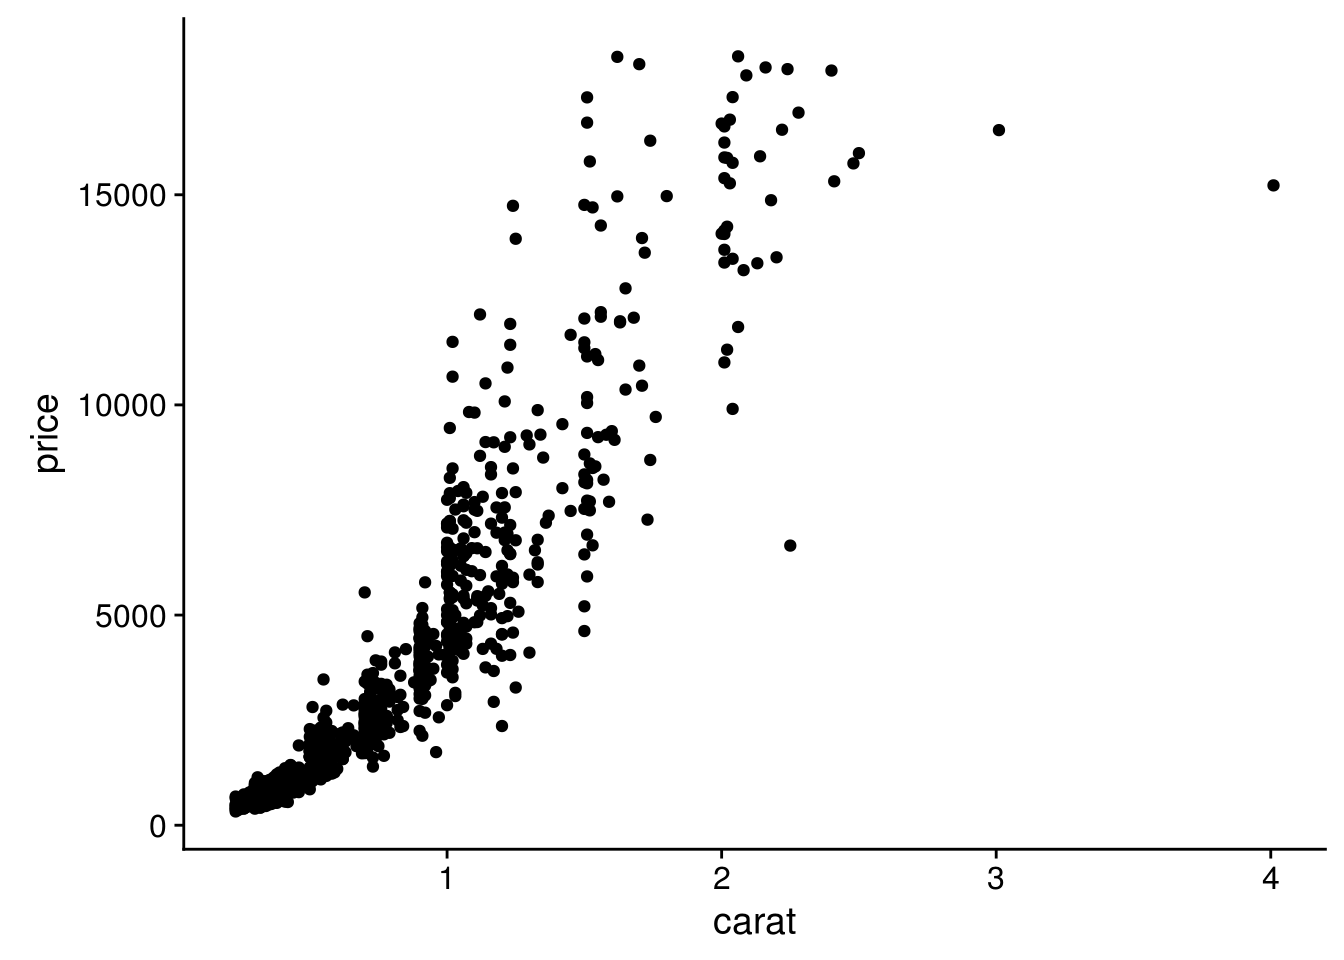
\includegraphics[width=0.95\linewidth,height=0.7\textheight,keepaspectratio]{R_course_files/figure-latex/unnamed-chunk-73-1} \end{center}

绘制散点图,对x,y值取log

\begin{Shaded}
\begin{Highlighting}[]
\KeywordTok{qplot}\NormalTok{(}\KeywordTok{log}\NormalTok{(carat),}\KeywordTok{log}\NormalTok{(price),}\DataTypeTok{data=}\NormalTok{dat)}
\end{Highlighting}
\end{Shaded}

\begin{center}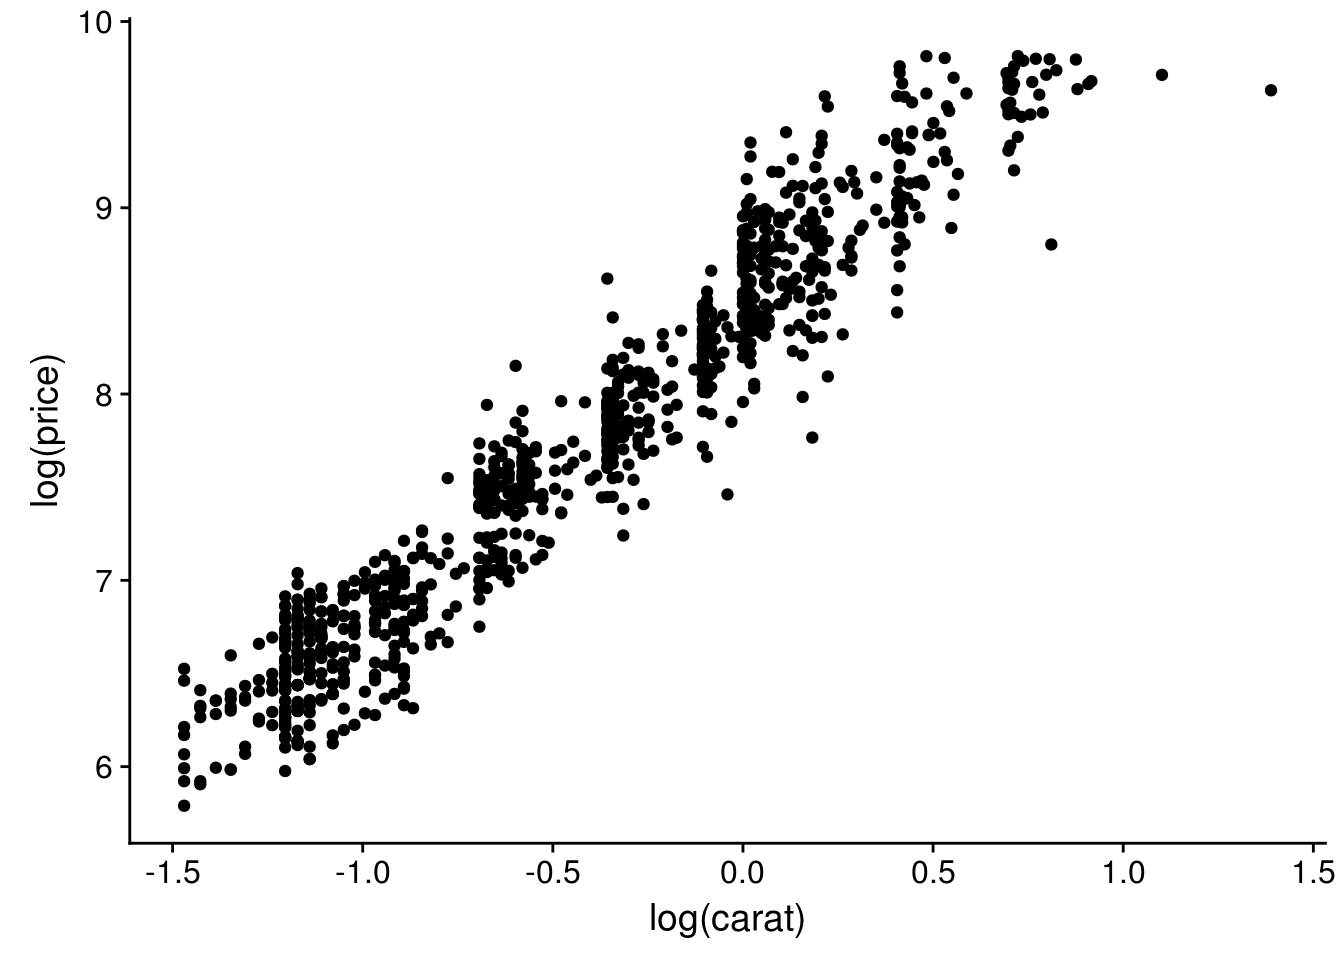
\includegraphics[width=0.95\linewidth,height=0.7\textheight,keepaspectratio]{R_course_files/figure-latex/unnamed-chunk-74-1} \end{center}

颜色、大小、性状和其他属性的设置

\begin{Shaded}
\begin{Highlighting}[]
\KeywordTok{qplot}\NormalTok{(carat,price,}\DataTypeTok{data=}\NormalTok{dat,}\DataTypeTok{colour=}\NormalTok{color)}
\end{Highlighting}
\end{Shaded}

\begin{center}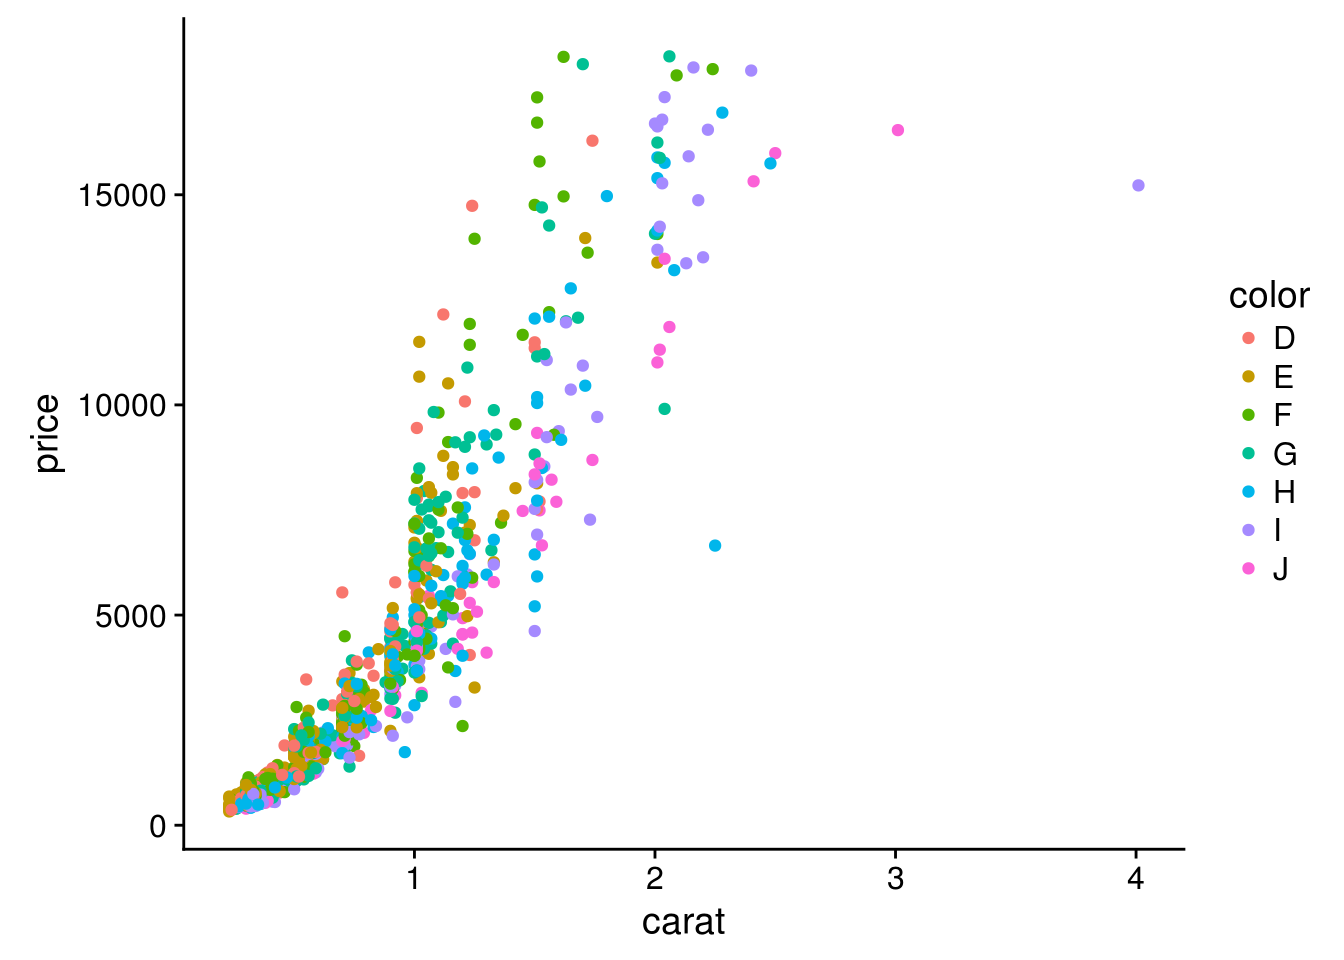
\includegraphics[width=0.95\linewidth,height=0.7\textheight,keepaspectratio]{R_course_files/figure-latex/unnamed-chunk-75-1} \end{center}

\begin{Shaded}
\begin{Highlighting}[]
\KeywordTok{qplot}\NormalTok{(carat,price,}\DataTypeTok{data=}\NormalTok{dat,}\DataTypeTok{shape=}\NormalTok{cut)}\CommentTok{#以cut为分类依据设置不同的形状}
\end{Highlighting}
\end{Shaded}

\begin{center}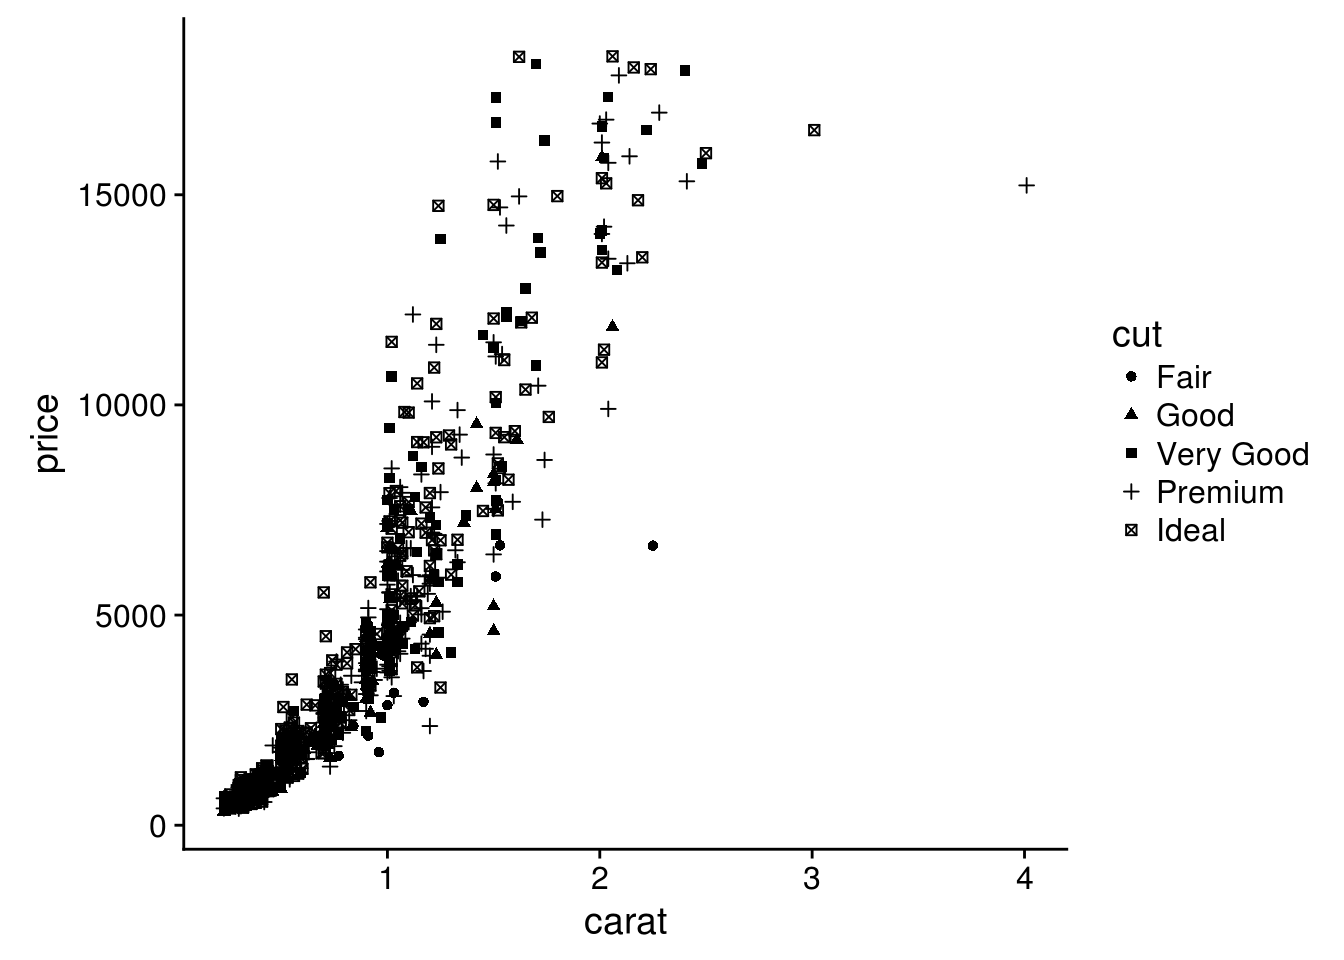
\includegraphics[width=0.95\linewidth,height=0.7\textheight,keepaspectratio]{R_course_files/figure-latex/unnamed-chunk-76-1} \end{center}

\textbf{几何对象}

\texttt{qplot()}函数配合不同的几何对象便可绘制出不同的图形:

\begin{itemize}
\tightlist
\item
  点图 \texttt{geom="point"}\\
\item
  平滑曲线 \texttt{geom="smooth"}\\
\item
  箱线图 \texttt{geom="boxplot"}
\item
  任意方向的路径性\texttt{geom="path"}\\
\item
  线条图 \texttt{geom="line"} (从左到右连接)
\item
  对于连续变量,直方图\texttt{geom="histogram"}\\
\item
  频率多边图 \texttt{geom="freqpoly"}
\item
  绘制密度曲线 \texttt{geom="density"}
\item
  如果只有x参数传递给qplot(),那么默认是直方图
\item
  对于离散变量,geom=``bar''绘制条形图
\end{itemize}

\begin{Shaded}
\begin{Highlighting}[]
\CommentTok{#向图形中加入平滑曲线(#从本张图片可以逐渐体会ggplot绘图的强大,}
\CommentTok{#后期应用ggplot()函数后,可以更加自由的绘制各种组合图形)}
\KeywordTok{qplot}\NormalTok{(carat,price,}\DataTypeTok{data=}\NormalTok{dat,}\DataTypeTok{geom=}\KeywordTok{c}\NormalTok{(}\StringTok{"point"}\NormalTok{,}\StringTok{"smooth"}\NormalTok{))}\CommentTok{#添加了一条拟合曲线}
\end{Highlighting}
\end{Shaded}

\begin{verbatim}
## `geom_smooth()` using method = 'gam'
\end{verbatim}

\begin{Shaded}
\begin{Highlighting}[]
\CommentTok{#拟合曲线默认的方法为method="loss",程序会根据数据点的多少自动选取,}
\CommentTok{#曲线周围的灰色部分为标准误,可以用se=FALSE曲线}
\end{Highlighting}
\end{Shaded}

\begin{center}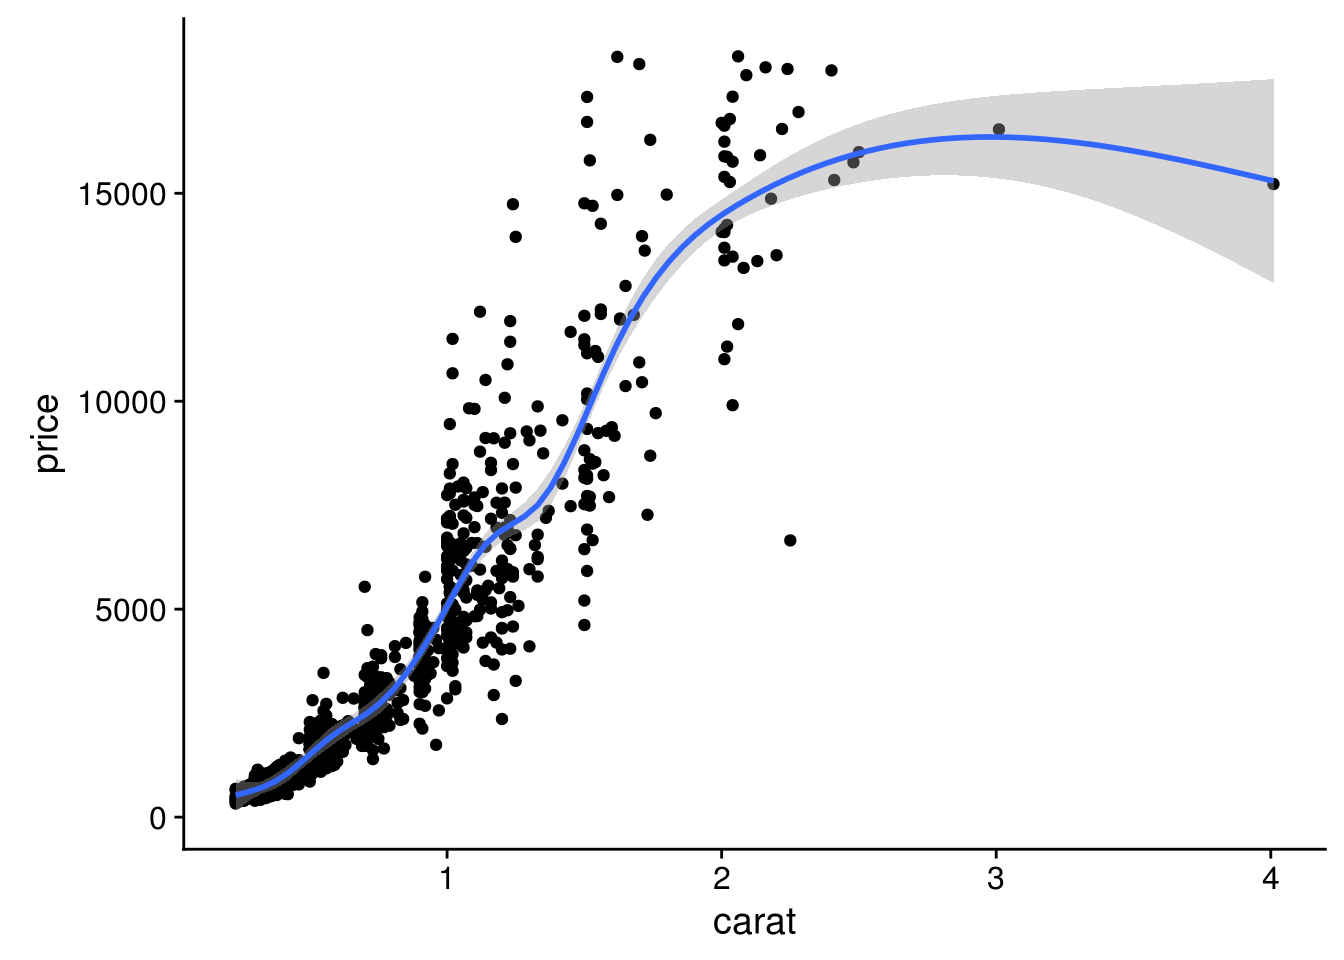
\includegraphics[width=0.95\linewidth,height=0.7\textheight,keepaspectratio]{R_course_files/figure-latex/unnamed-chunk-77-1} \end{center}

\textbf{绘制其他常见图形}

\begin{enumerate}
\def\labelenumi{\arabic{enumi}.}
\tightlist
\item
  箱线图
\end{enumerate}

\begin{Shaded}
\begin{Highlighting}[]
\KeywordTok{qplot}\NormalTok{(color,price/carat,}\DataTypeTok{data=}\NormalTok{dat,}\DataTypeTok{geom=}\StringTok{"boxplot"}\NormalTok{)}
\end{Highlighting}
\end{Shaded}

\begin{center}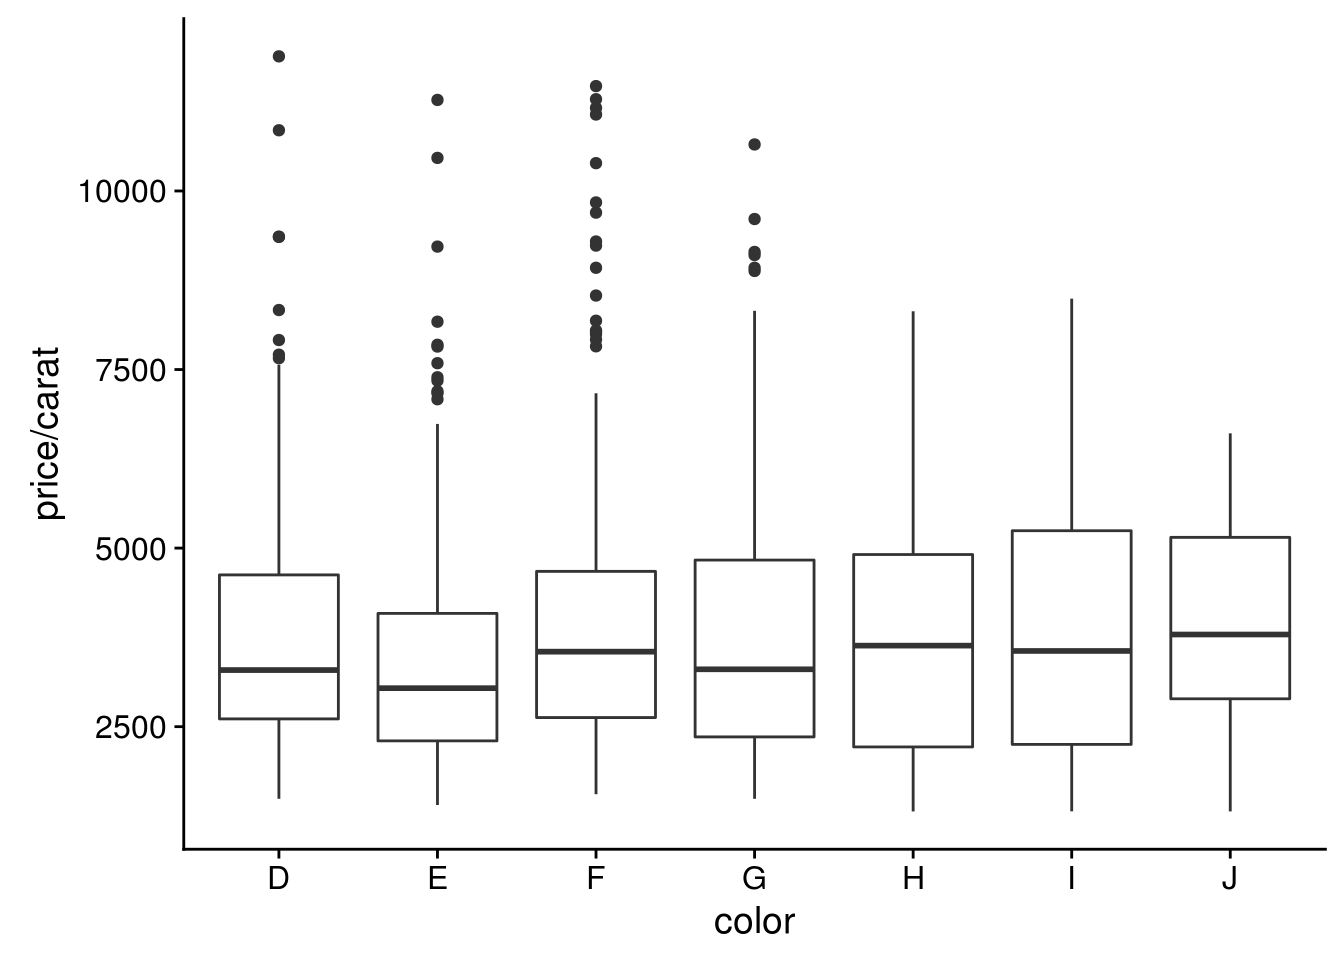
\includegraphics[width=0.95\linewidth,height=0.7\textheight,keepaspectratio]{R_course_files/figure-latex/unnamed-chunk-78-1} \end{center}

\begin{enumerate}
\def\labelenumi{\arabic{enumi}.}
\setcounter{enumi}{1}
\tightlist
\item
  绕动图 (抖动图)
\end{enumerate}

\begin{Shaded}
\begin{Highlighting}[]
\KeywordTok{qplot}\NormalTok{(color,price/carat,}\DataTypeTok{data=}\NormalTok{diamonds,}\DataTypeTok{geom=}\StringTok{"jitter"}\NormalTok{)}
\end{Highlighting}
\end{Shaded}

\begin{center}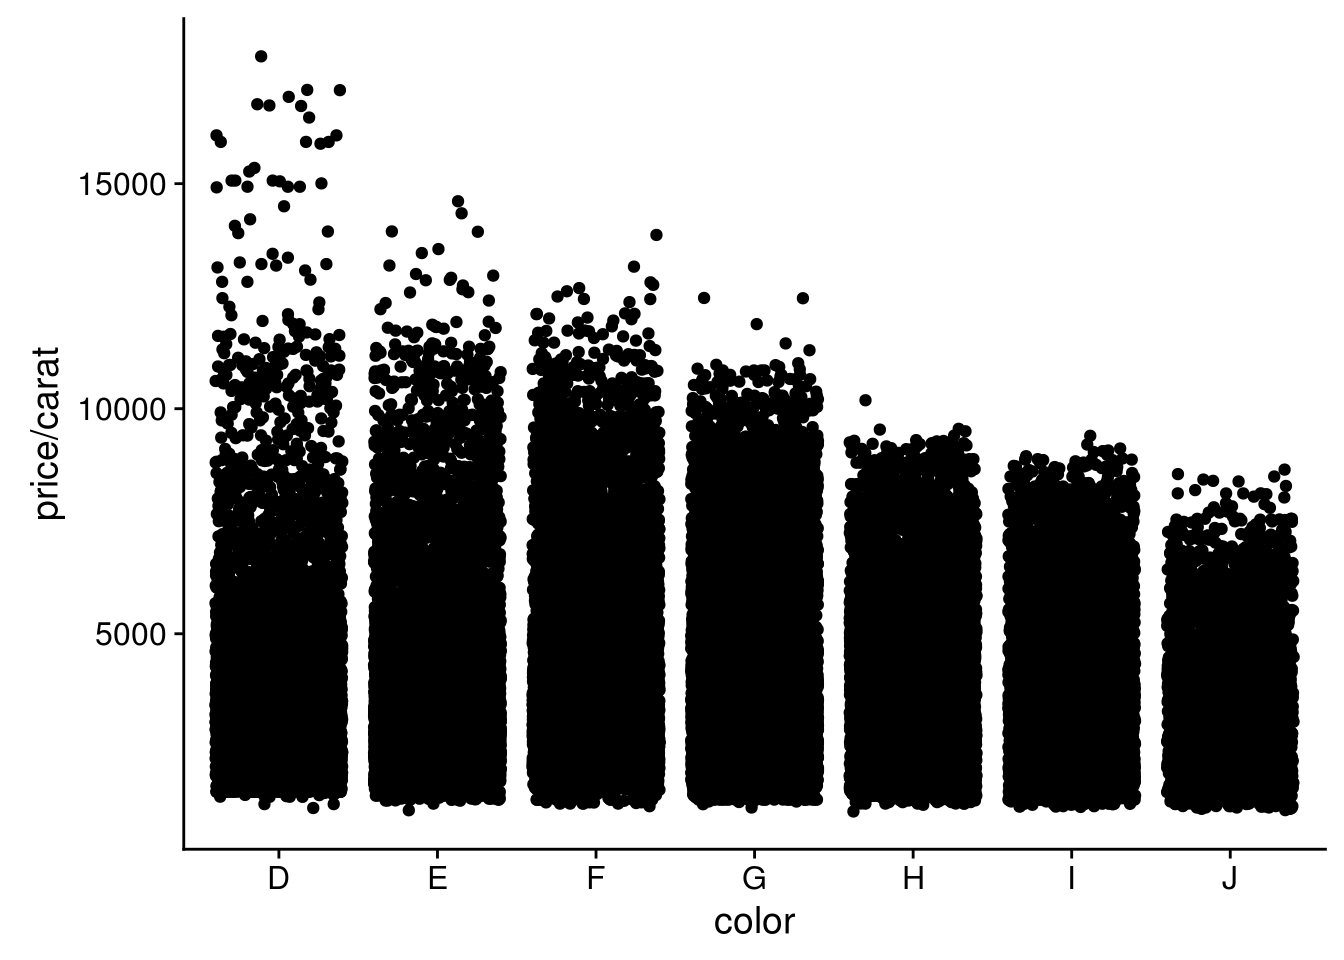
\includegraphics[width=0.95\linewidth,height=0.7\textheight,keepaspectratio]{R_course_files/figure-latex/unnamed-chunk-79-1} \end{center}

\begin{enumerate}
\def\labelenumi{\arabic{enumi}.}
\setcounter{enumi}{2}
\tightlist
\item
  直方图
\end{enumerate}

\begin{Shaded}
\begin{Highlighting}[]
\KeywordTok{qplot}\NormalTok{(carat,}\DataTypeTok{data=}\NormalTok{dat,}\DataTypeTok{geom=}\StringTok{"histogram"}\NormalTok{)}
\end{Highlighting}
\end{Shaded}

\begin{verbatim}
## `stat_bin()` using `bins = 30`. Pick better value with `binwidth`.
\end{verbatim}

\begin{center}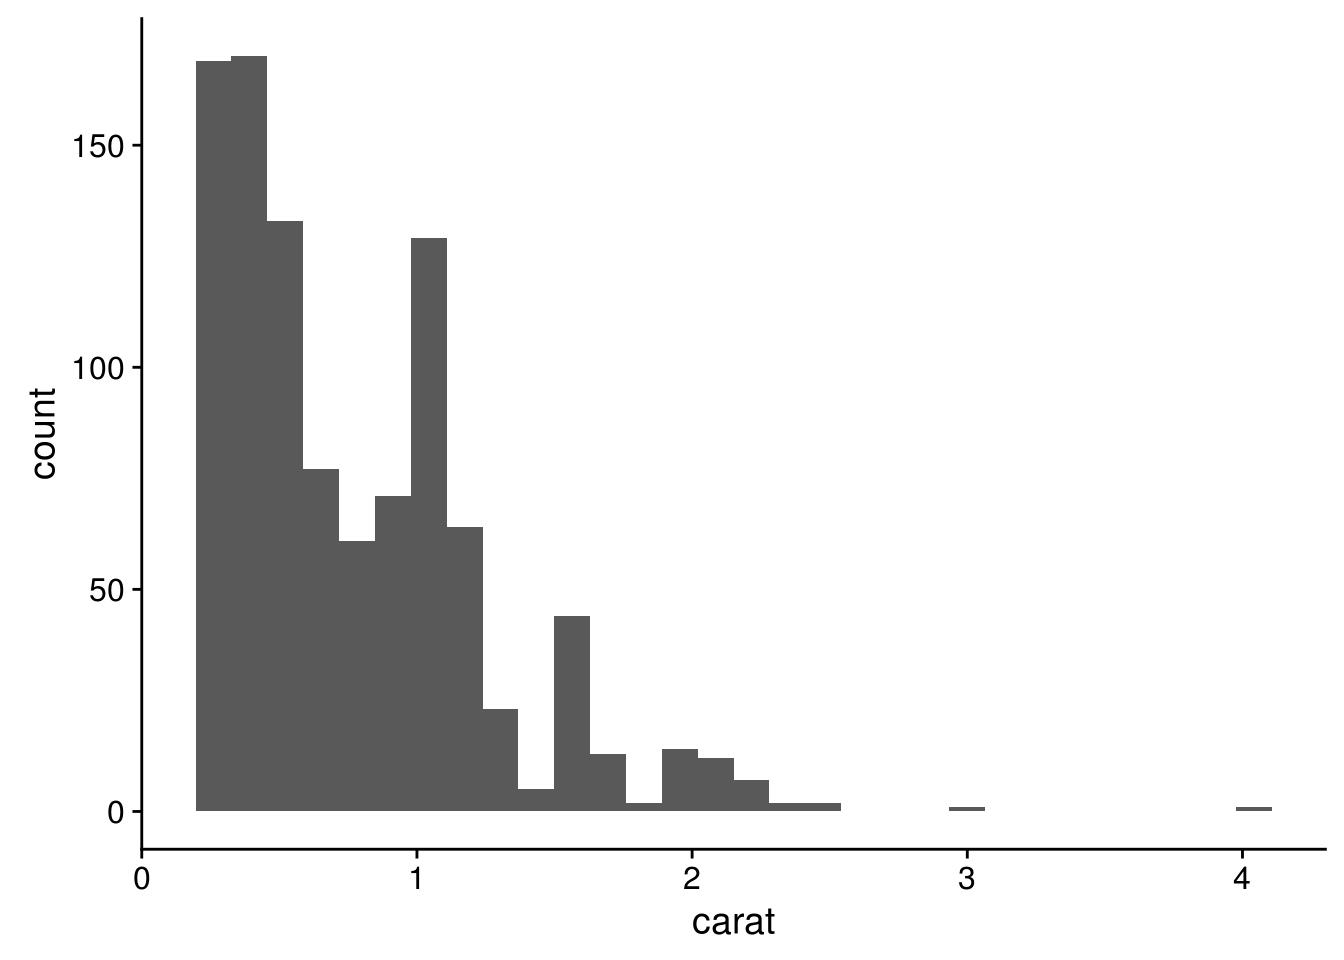
\includegraphics[width=0.95\linewidth,height=0.7\textheight,keepaspectratio]{R_course_files/figure-latex/unnamed-chunk-80-1} \end{center}

\begin{enumerate}
\def\labelenumi{\arabic{enumi}.}
\setcounter{enumi}{3}
\tightlist
\item
  密度曲线图
\end{enumerate}

\begin{Shaded}
\begin{Highlighting}[]
\KeywordTok{qplot}\NormalTok{(carat,}\DataTypeTok{data=}\NormalTok{dat,}\DataTypeTok{geom=}\StringTok{"density"}\NormalTok{)}
\end{Highlighting}
\end{Shaded}

\begin{center}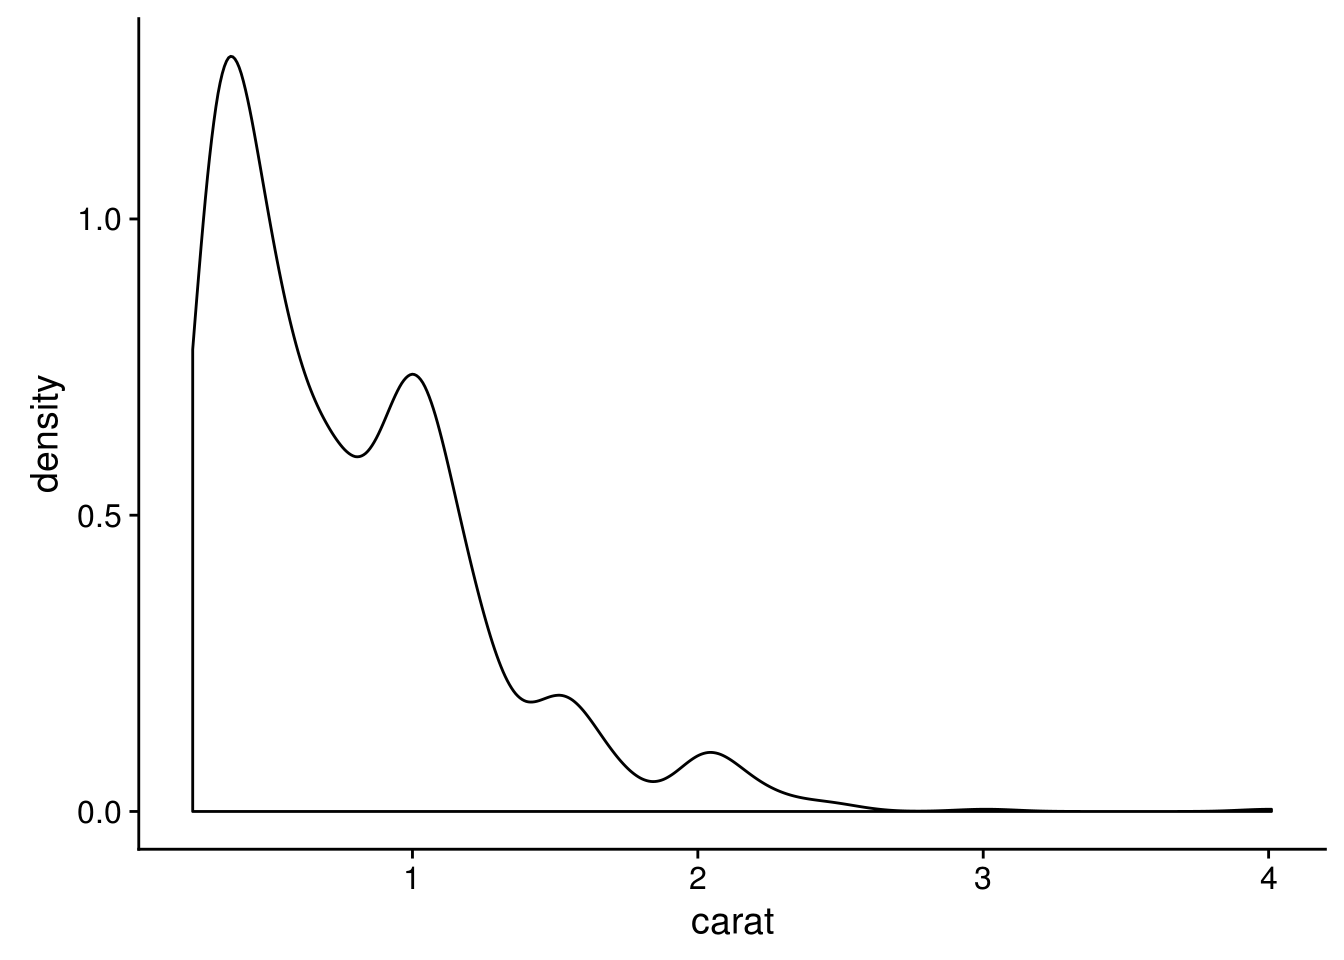
\includegraphics[width=0.95\linewidth,height=0.7\textheight,keepaspectratio]{R_course_files/figure-latex/unnamed-chunk-81-1} \end{center}

\begin{enumerate}
\def\labelenumi{\arabic{enumi}.}
\setcounter{enumi}{4}
\tightlist
\item
  条形图
\end{enumerate}

\begin{Shaded}
\begin{Highlighting}[]
\KeywordTok{qplot}\NormalTok{(color,}\DataTypeTok{data=}\NormalTok{dat,}\DataTypeTok{geom=}\StringTok{"bar"}\NormalTok{)}
\end{Highlighting}
\end{Shaded}

\begin{center}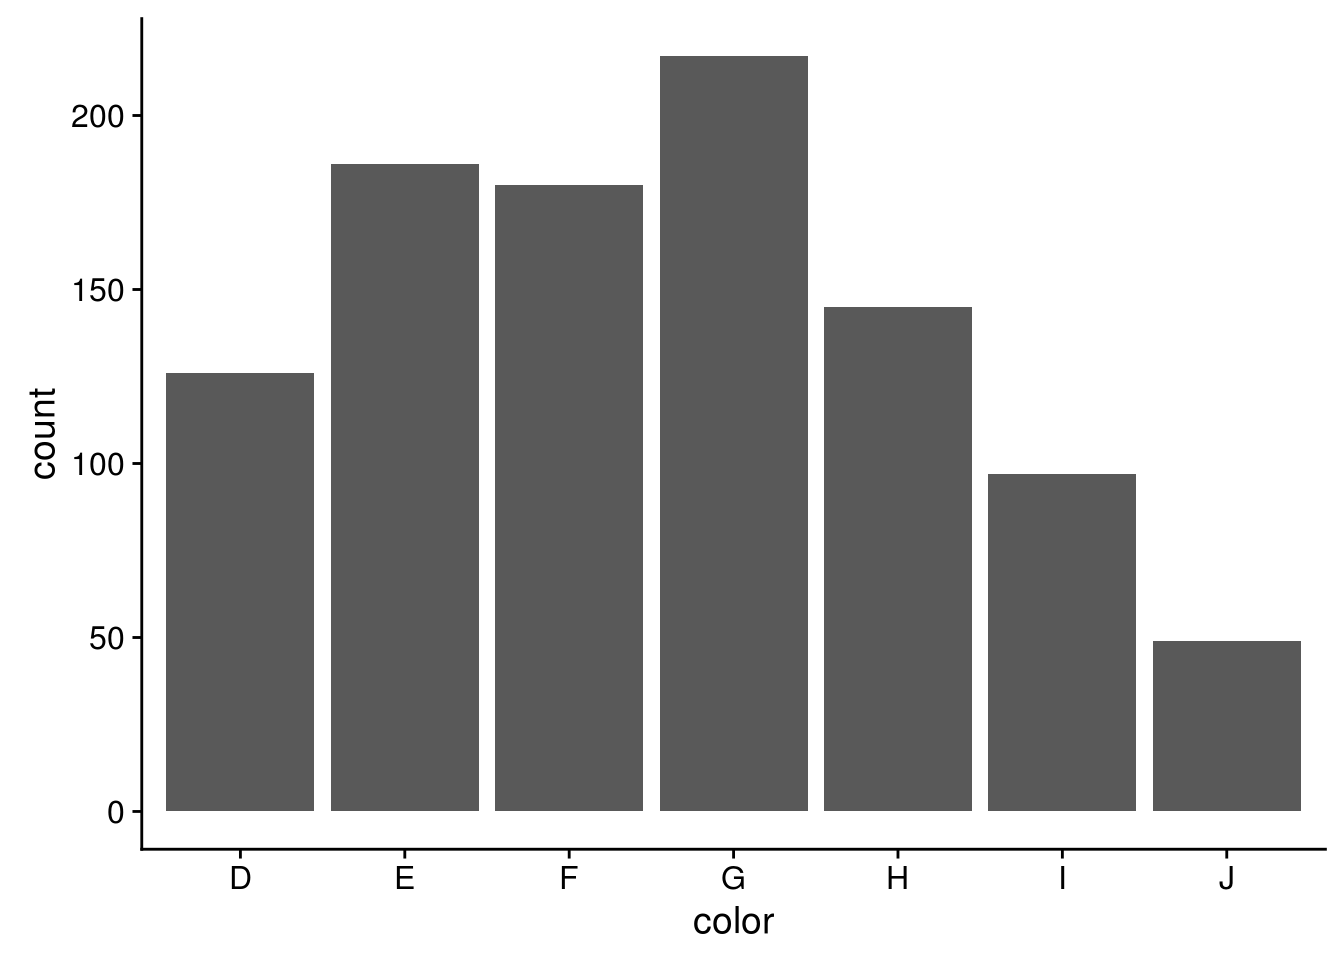
\includegraphics[width=0.95\linewidth,height=0.7\textheight,keepaspectratio]{R_course_files/figure-latex/unnamed-chunk-82-1} \end{center}

\begin{enumerate}
\def\labelenumi{\arabic{enumi}.}
\setcounter{enumi}{5}
\tightlist
\item
  时间序列线条图,采用另一个数据集economics
\end{enumerate}

\begin{Shaded}
\begin{Highlighting}[]
\KeywordTok{qplot}\NormalTok{(date,unemploy/pop,}\DataTypeTok{data=}\NormalTok{economics,}\DataTypeTok{geom=}\StringTok{"line"}\NormalTok{)}
\end{Highlighting}
\end{Shaded}

\begin{center}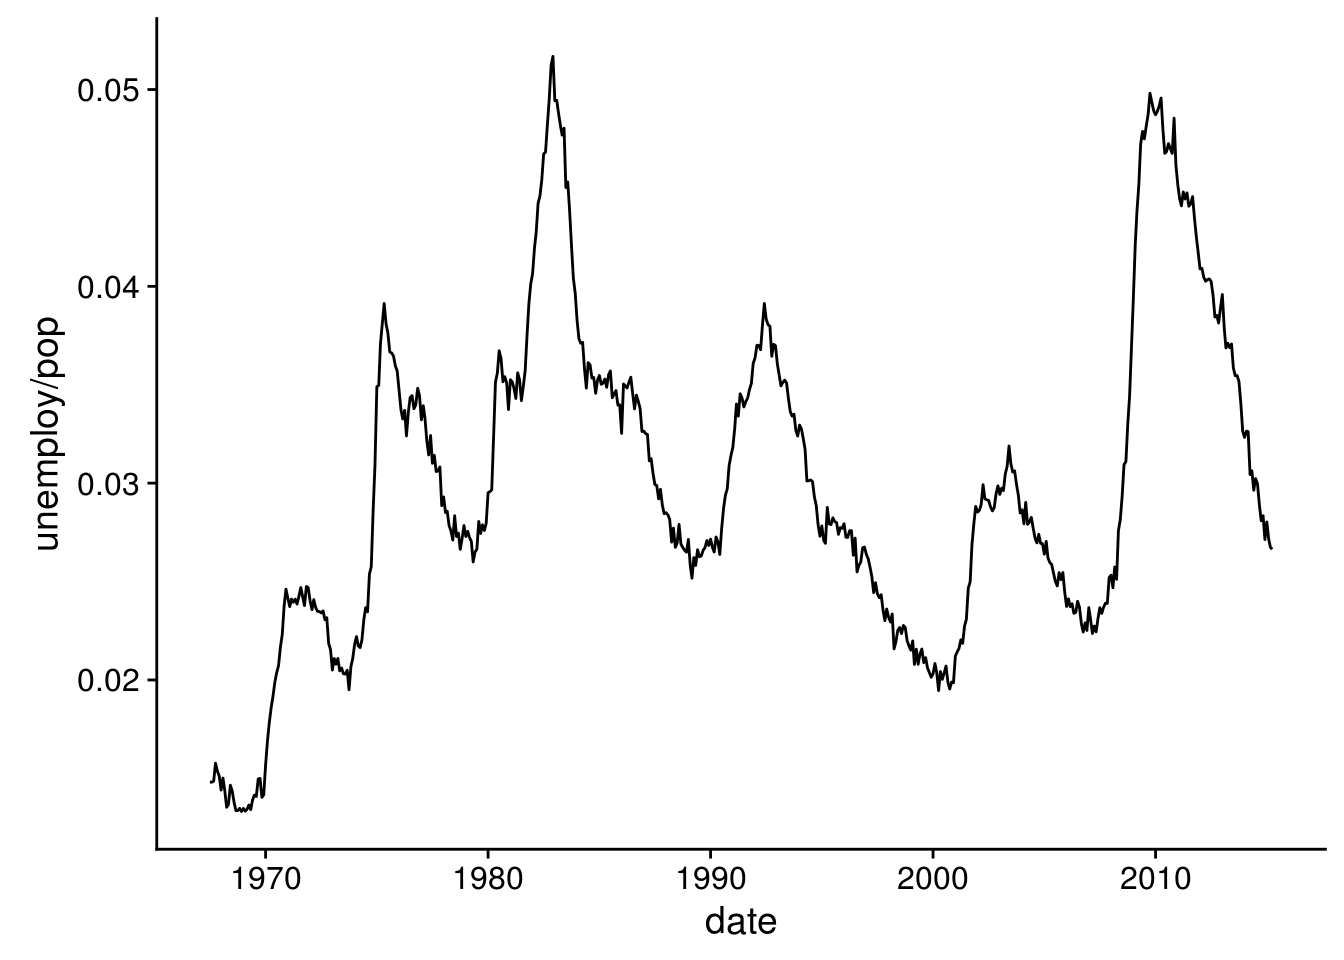
\includegraphics[width=0.95\linewidth,height=0.7\textheight,keepaspectratio]{R_course_files/figure-latex/unnamed-chunk-83-1} \end{center}

\begin{enumerate}
\def\labelenumi{\arabic{enumi}.}
\setcounter{enumi}{6}
\tightlist
\item
  分面绘图\texttt{facet}=分类变量
\end{enumerate}

\begin{Shaded}
\begin{Highlighting}[]
\KeywordTok{qplot}\NormalTok{(carat,}\DataTypeTok{data=}\NormalTok{dat,}\DataTypeTok{facets=}\NormalTok{color ~}\StringTok{ }\NormalTok{.,}\DataTypeTok{geom=}\StringTok{"histogram"}\NormalTok{,}\DataTypeTok{binwidth=}\FloatTok{0.1}\NormalTok{,}\DataTypeTok{xlim=}\KeywordTok{c}\NormalTok{(}\DecValTok{0}\NormalTok{,}\DecValTok{3}\NormalTok{))}
\end{Highlighting}
\end{Shaded}

\begin{center}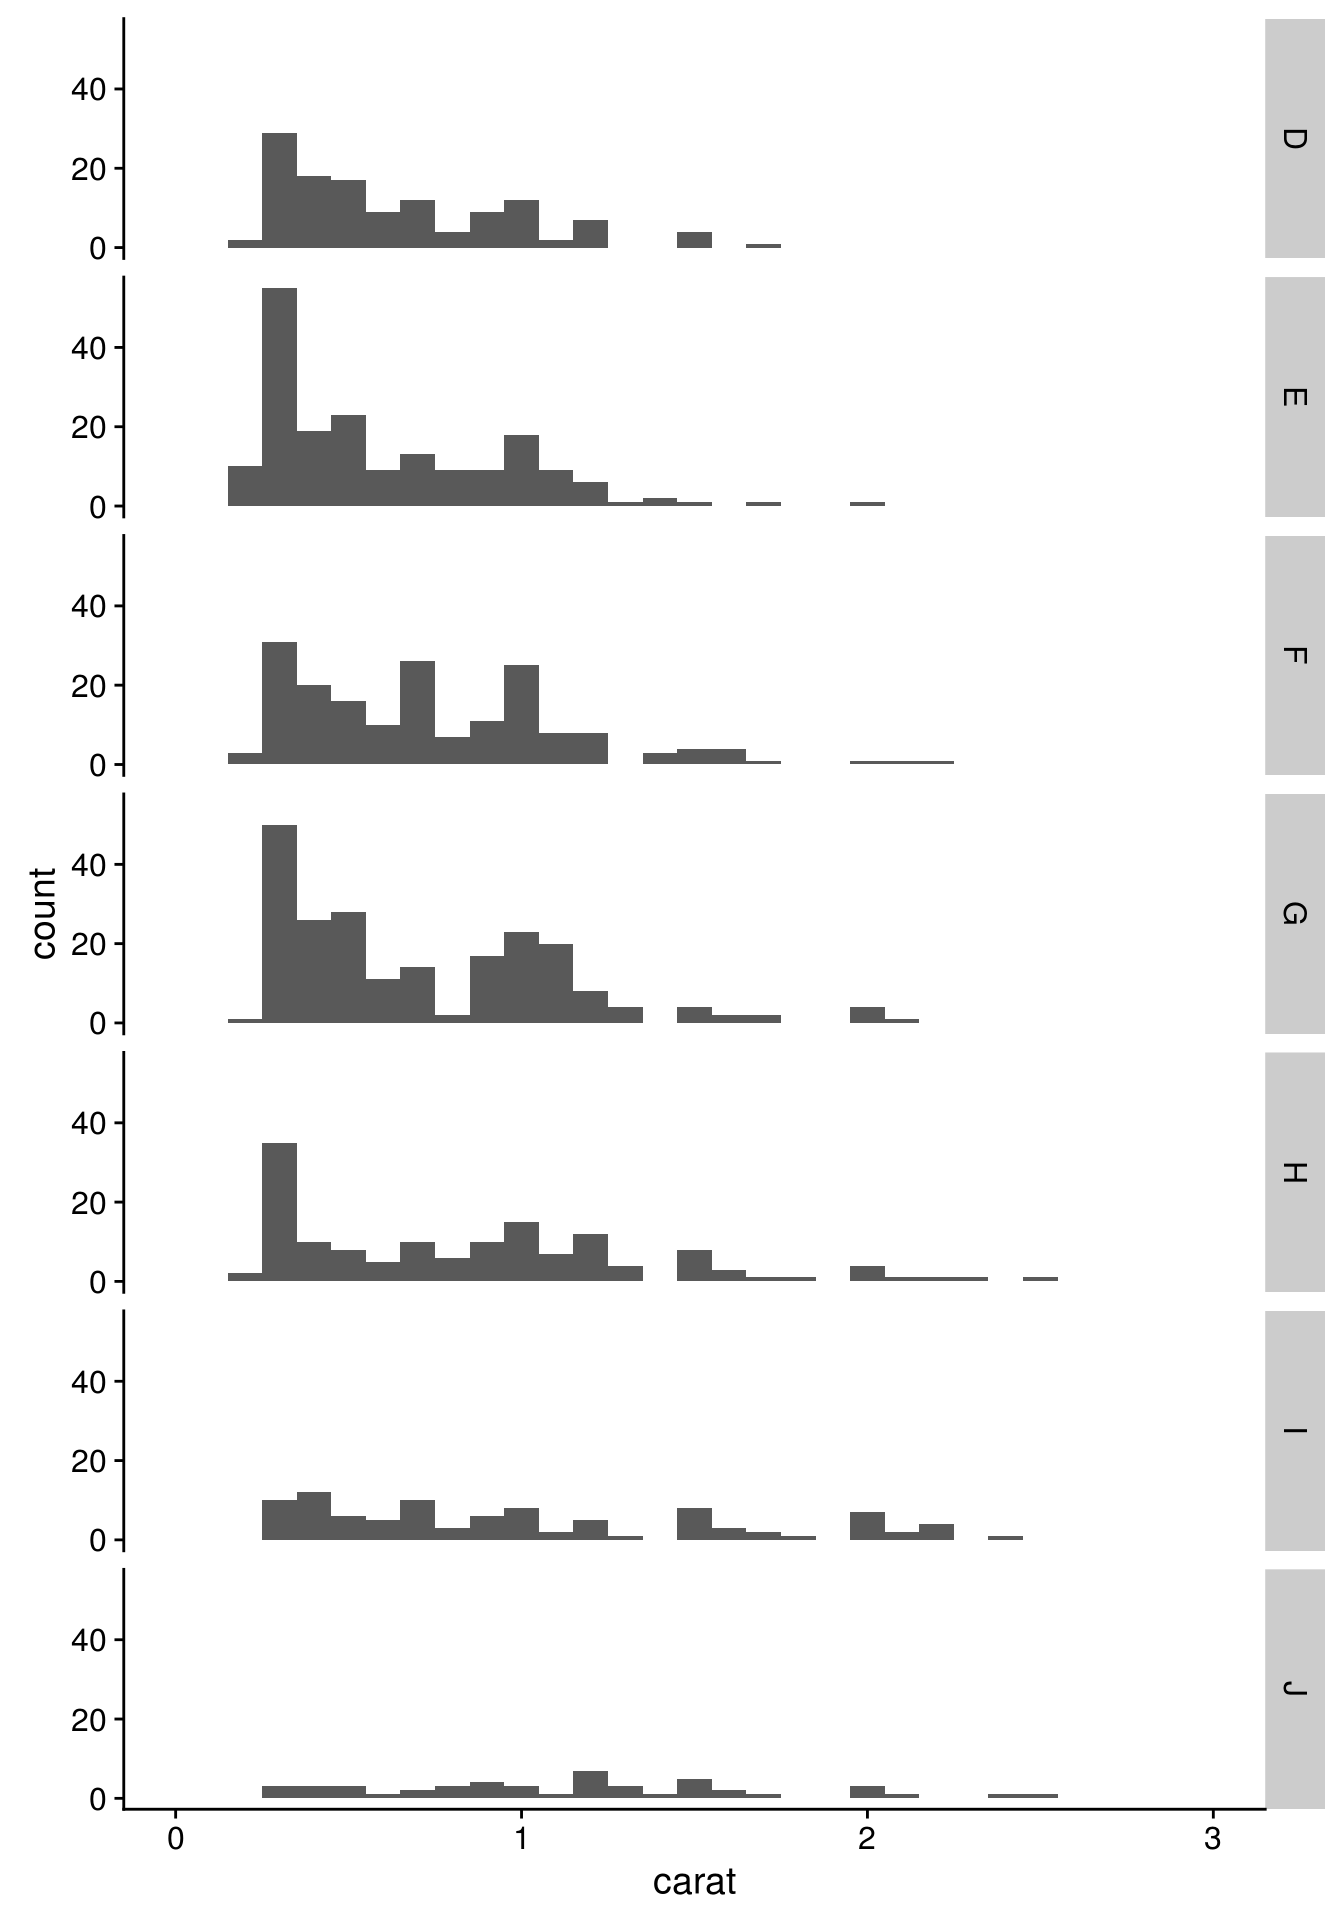
\includegraphics[width=0.95\linewidth,height=0.7\textheight,keepaspectratio]{R_course_files/figure-latex/unnamed-chunk-84-1} \end{center}

以上为ggplot2包中常见图形的快速绘制
(\texttt{quickplot})即\texttt{qplot}函数的应用。
\texttt{qplot}函数还有很多其他的参数,
对\texttt{xlim},\texttt{ylim}设置\texttt{x},\texttt{y}轴的区间例如\texttt{xlim=c(0,20)};
对轴取\texttt{log}值,\texttt{log="x"},对x轴取对数,\texttt{log="xy"}表示对x轴和y轴取对数;main:图形的主题main=``qplot
title''; \#xlab,ylab:设置轴标签文字

\begin{Shaded}
\begin{Highlighting}[]
\KeywordTok{qplot}\NormalTok{(carat,price,}\DataTypeTok{data=}\NormalTok{dat,}
     \DataTypeTok{xlab=}\StringTok{"Price($)"}\NormalTok{,}\DataTypeTok{ylab=}\StringTok{"Weight(carat)"}\NormalTok{,}
     \DataTypeTok{main=}\StringTok{"Price-Weight relationship"}\NormalTok{)}
\end{Highlighting}
\end{Shaded}

\begin{center}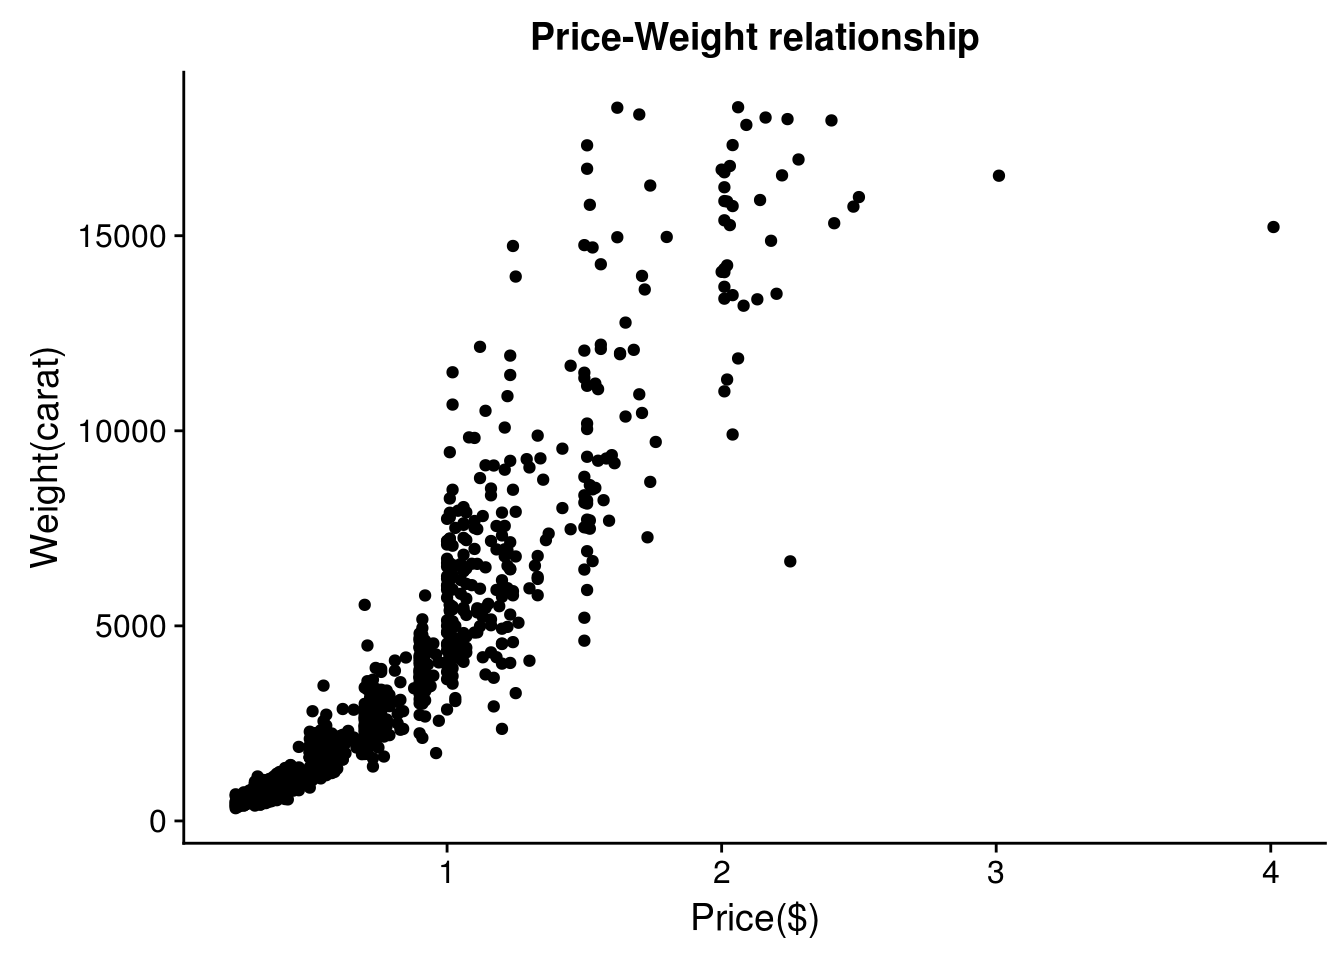
\includegraphics[width=0.95\linewidth,height=0.7\textheight,keepaspectratio]{R_course_files/figure-latex/unnamed-chunk-85-1} \end{center}

\subsection{热图绘制}

热图是做分析时常用的展示方式,简单、直观、清晰。可以用来显示基因在不同样品中表达的高低、表观修饰水平的高低、样品之间的相关性等。任何一个数值矩阵都可以通过合适的方式用热图展示。

本篇使用R的\texttt{ggplot2}包实现从原始数据读入到热图输出的过程,并在教程结束后提供一份封装好的命令行绘图工具,只需要提供矩阵,即可一键绘图。

上一篇讲述了Rstudio的使用作为R写作和编译环境的入门,后面的命令都可以拷贝到Rstudio中运行,或写成一个R脚本,使用\texttt{Rscript\ heatmap.r}运行。我们还提供了Bash的封装,在不修改R脚本的情况下,改变参数绘制出不同的图形。

\subsubsection{生成测试数据}

绘图首先需要数据。通过生成几组向量,转换为矩阵,得到想要的数据。

\begin{Shaded}
\begin{Highlighting}[]
\NormalTok{data <-}\StringTok{ }\KeywordTok{c}\NormalTok{(}\DecValTok{1}\NormalTok{:}\DecValTok{6}\NormalTok{,}\DecValTok{6}\NormalTok{:}\DecValTok{1}\NormalTok{,}\DecValTok{6}\NormalTok{:}\DecValTok{1}\NormalTok{,}\DecValTok{1}\NormalTok{:}\DecValTok{6}\NormalTok{, (}\DecValTok{6}\NormalTok{:}\DecValTok{1}\NormalTok{)/}\DecValTok{10}\NormalTok{,(}\DecValTok{1}\NormalTok{:}\DecValTok{6}\NormalTok{)/}\DecValTok{10}\NormalTok{,(}\DecValTok{1}\NormalTok{:}\DecValTok{6}\NormalTok{)/}\DecValTok{10}\NormalTok{,(}\DecValTok{6}\NormalTok{:}\DecValTok{1}\NormalTok{)/}\DecValTok{10}\NormalTok{,}\DecValTok{1}\NormalTok{:}\DecValTok{6}\NormalTok{,}\DecValTok{6}\NormalTok{:}\DecValTok{1}\NormalTok{,}\DecValTok{6}\NormalTok{:}\DecValTok{1}\NormalTok{,}\DecValTok{1}\NormalTok{:}\DecValTok{6}\NormalTok{,}
        \DecValTok{6}\NormalTok{:}\DecValTok{1}\NormalTok{,}\DecValTok{1}\NormalTok{:}\DecValTok{6}\NormalTok{,}\DecValTok{1}\NormalTok{:}\DecValTok{6}\NormalTok{,}\DecValTok{6}\NormalTok{:}\DecValTok{1}\NormalTok{)}
\NormalTok{data}
\end{Highlighting}
\end{Shaded}

\begin{verbatim}
##  [1] 1.0 2.0 3.0 4.0 5.0 6.0 6.0 5.0 4.0 3.0 2.0 1.0 6.0 5.0 4.0 3.0 2.0
## [18] 1.0 1.0 2.0 3.0 4.0 5.0 6.0 0.6 0.5 0.4 0.3 0.2 0.1 0.1 0.2 0.3 0.4
## [35] 0.5 0.6 0.1 0.2 0.3 0.4 0.5 0.6 0.6 0.5 0.4 0.3 0.2 0.1 1.0 2.0 3.0
## [52] 4.0 5.0 6.0 6.0 5.0 4.0 3.0 2.0 1.0 6.0 5.0 4.0 3.0 2.0 1.0 1.0 2.0
## [69] 3.0 4.0 5.0 6.0 6.0 5.0 4.0 3.0 2.0 1.0 1.0 2.0 3.0 4.0 5.0 6.0 1.0
## [86] 2.0 3.0 4.0 5.0 6.0 6.0 5.0 4.0 3.0 2.0 1.0
\end{verbatim}

\textbf{注意}:运算符的优先级。

\begin{Shaded}
\begin{Highlighting}[]
\DecValTok{1}\NormalTok{:}\DecValTok{3+4}
\end{Highlighting}
\end{Shaded}

\begin{verbatim}
## [1] 5 6 7
\end{verbatim}

\begin{Shaded}
\begin{Highlighting}[]
\NormalTok{(}\DecValTok{1}\NormalTok{:}\DecValTok{3}\NormalTok{)+}\DecValTok{4}
\end{Highlighting}
\end{Shaded}

\begin{verbatim}
## [1] 5 6 7
\end{verbatim}

\begin{Shaded}
\begin{Highlighting}[]
\DecValTok{1}\NormalTok{:(}\DecValTok{3+4}\NormalTok{)}
\end{Highlighting}
\end{Shaded}

\begin{verbatim}
## [1] 1 2 3 4 5 6 7
\end{verbatim}

Vector转为矩阵 (matrix),再转为数据框 (data.frame)。

\begin{Shaded}
\begin{Highlighting}[]
\CommentTok{# ncol: 指定列数}
\CommentTok{# byrow: 先按行填充数据}
\CommentTok{# ?matrix 可查看函数的使用方法}
\CommentTok{# as.data.frame的as系列是转换用的}
\NormalTok{data <-}\StringTok{ }\KeywordTok{as.data.frame}\NormalTok{(}\KeywordTok{matrix}\NormalTok{(data, }\DataTypeTok{ncol=}\DecValTok{12}\NormalTok{, }\DataTypeTok{byrow=}\NormalTok{T))}
\NormalTok{data}
\end{Highlighting}
\end{Shaded}

\begin{verbatim}
##    V1  V2  V3  V4  V5  V6  V7  V8  V9 V10 V11 V12
## 1 1.0 2.0 3.0 4.0 5.0 6.0 6.0 5.0 4.0 3.0 2.0 1.0
## 2 6.0 5.0 4.0 3.0 2.0 1.0 1.0 2.0 3.0 4.0 5.0 6.0
## 3 0.6 0.5 0.4 0.3 0.2 0.1 0.1 0.2 0.3 0.4 0.5 0.6
## 4 0.1 0.2 0.3 0.4 0.5 0.6 0.6 0.5 0.4 0.3 0.2 0.1
## 5 1.0 2.0 3.0 4.0 5.0 6.0 6.0 5.0 4.0 3.0 2.0 1.0
## 6 6.0 5.0 4.0 3.0 2.0 1.0 1.0 2.0 3.0 4.0 5.0 6.0
## 7 6.0 5.0 4.0 3.0 2.0 1.0 1.0 2.0 3.0 4.0 5.0 6.0
## 8 1.0 2.0 3.0 4.0 5.0 6.0 6.0 5.0 4.0 3.0 2.0 1.0
\end{verbatim}

\begin{Shaded}
\begin{Highlighting}[]
\CommentTok{# 增加列的名字}
\KeywordTok{colnames}\NormalTok{(data) <-}\StringTok{ }\KeywordTok{c}\NormalTok{(}\StringTok{"Zygote"}\NormalTok{,}\StringTok{"2_cell"}\NormalTok{,}\StringTok{"4_cell"}\NormalTok{,}\StringTok{"8_cell"}\NormalTok{,}\StringTok{"Morula"}\NormalTok{,}\StringTok{"ICM"}\NormalTok{,}\StringTok{"ESC"}\NormalTok{,}
        \StringTok{"4 week PGC"}\NormalTok{,}\StringTok{"7 week PGC"}\NormalTok{,}\StringTok{"10 week PGC"}\NormalTok{,}\StringTok{"17 week PGC"}\NormalTok{, }\StringTok{"OOcyte"}\NormalTok{)}

\CommentTok{# 增加行的名字}
\CommentTok{# 注意paste和paste0的使用}
\KeywordTok{rownames}\NormalTok{(data) <-}\StringTok{ }\KeywordTok{paste}\NormalTok{(}\StringTok{"Gene"}\NormalTok{, }\DecValTok{1}\NormalTok{:}\DecValTok{8}\NormalTok{, }\DataTypeTok{sep=}\StringTok{"_"}\NormalTok{)}

\CommentTok{# 只显示前6行和前4列}
\KeywordTok{head}\NormalTok{(data)[,}\DecValTok{1}\NormalTok{:}\DecValTok{4}\NormalTok{]}
\end{Highlighting}
\end{Shaded}

\begin{verbatim}
##        Zygote 2_cell 4_cell 8_cell
## Gene_1    1.0    2.0    3.0    4.0
## Gene_2    6.0    5.0    4.0    3.0
## Gene_3    0.6    0.5    0.4    0.3
## Gene_4    0.1    0.2    0.3    0.4
## Gene_5    1.0    2.0    3.0    4.0
## Gene_6    6.0    5.0    4.0    3.0
\end{verbatim}

虽然方法比较繁琐,但一个数值矩阵已经获得了。

还有另外2种获取数值矩阵的方式。

\begin{itemize}
\tightlist
\item
  读入字符串
\end{itemize}

\begin{Shaded}
\begin{Highlighting}[]
\CommentTok{# 使用字符串的好处是不需要额外提供文件}
\CommentTok{# 简单测试时可使用,写起来不繁琐,又方便重复}
\CommentTok{# 尤其适用于在线提问时作为测试案例}
\NormalTok{txt <-}\StringTok{ "ID;Zygote;2_cell;4_cell;8_cell}
\StringTok{+ Gene_1;1;2;3;4}
\StringTok{+ Gene_2;6;5;4;5}
\StringTok{+ Gene_3;0.6;0.5;0.4;0.4"}

\CommentTok{# 习惯设置quote为空,避免部分基因名字或注释中存在引号,导致读入文件错误。}
\CommentTok{# 具体错误可查看 http://blog.genesino.com/collections/R_tips/ 中的记录}
\NormalTok{data2 <-}\StringTok{ }\KeywordTok{read.table}\NormalTok{(}\DataTypeTok{text=}\NormalTok{txt,}\DataTypeTok{sep=}\StringTok{";"}\NormalTok{, }\DataTypeTok{header=}\NormalTok{T, }\DataTypeTok{row.names=}\DecValTok{1}\NormalTok{, }\DataTypeTok{quote=}\StringTok{""}\NormalTok{)}
\KeywordTok{head}\NormalTok{(data2)}
\end{Highlighting}
\end{Shaded}

\begin{verbatim}
##          Zygote X2_cell X4_cell X8_cell
## + Gene_1    1.0     2.0     3.0     4.0
## + Gene_2    6.0     5.0     4.0     5.0
## + Gene_3    0.6     0.5     0.4     0.4
\end{verbatim}

可以看到列名字中以数字开头的列都加了\textbf{X}。一般要尽量避免行或列名字以\textbf{数字开头},会给后续分析带来匹配问题;另外名字中出现的非字母、数字、下划线、点的字符都会被转为\textbf{点},也需要注意,尽量只用字母、下划线和数字。

\begin{Shaded}
\begin{Highlighting}[]
\CommentTok{# 读入时,增加一个参数`check.names=F`也可以解决问题。}
\CommentTok{# 这次数字前没有再加 X 了}
\NormalTok{data2 <-}\StringTok{ }\KeywordTok{read.table}\NormalTok{(}\DataTypeTok{text=}\NormalTok{txt,}\DataTypeTok{sep=}\StringTok{";"}\NormalTok{, }\DataTypeTok{header=}\NormalTok{T, }\DataTypeTok{row.names=}\DecValTok{1}\NormalTok{, }\DataTypeTok{quote=}\StringTok{""}\NormalTok{, }\DataTypeTok{check.names =} \NormalTok{F)}
\KeywordTok{head}\NormalTok{(data2)}
\end{Highlighting}
\end{Shaded}

\begin{verbatim}
##          Zygote 2_cell 4_cell 8_cell
## + Gene_1    1.0    2.0    3.0    4.0
## + Gene_2    6.0    5.0    4.0    5.0
## + Gene_3    0.6    0.5    0.4    0.4
\end{verbatim}

\begin{itemize}
\tightlist
\item
  读入文件
\end{itemize}

与上一步类似,只是把\texttt{txt}代表的文字存到文件中,再利用文件名读取,不再赘述。

\begin{Shaded}
\begin{Highlighting}[]
\CommentTok{#data2 <- read.table("filename",sep=";", header=T, row.names=1, quote="")}
\end{Highlighting}
\end{Shaded}

\subsubsection{转换数据格式}

数据读入后,还需要一步格式转换。在使用ggplot2作图时,有一种长表格模式是最为常用的,尤其是数据不规则时,更应该使用
(这点,我们在讲解箱线图时再说)。

\texttt{melt}:把正常矩阵转换为长表格模式的函数。工作原理是把全部的非id列的\texttt{数值列}转为1列
(列名默认为\texttt{value});所有字符列转为一列,列名默认为\texttt{variable}。

\begin{Shaded}
\begin{Highlighting}[]
\CommentTok{# 如果包没有安装,运行下面一句,安装包}
\CommentTok{#install.packages(c("reshape2","ggplot2"))}

\KeywordTok{library}\NormalTok{(reshape2)}
\KeywordTok{library}\NormalTok{(ggplot2)}

\CommentTok{# 转换前,先增加一列ID列,保存行名字}
\NormalTok{data$ID <-}\StringTok{ }\KeywordTok{rownames}\NormalTok{(data)}


\CommentTok{# id.vars 列用于指定哪些列为id列;这些列不会被merge,会保留为完整一列。}
\NormalTok{data_m <-}\StringTok{ }\KeywordTok{melt}\NormalTok{(data, }\DataTypeTok{id.vars=}\KeywordTok{c}\NormalTok{(}\StringTok{"ID"}\NormalTok{))}
\KeywordTok{head}\NormalTok{(data_m)}
\end{Highlighting}
\end{Shaded}

\begin{verbatim}
##       ID variable value
## 1 Gene_1   Zygote   1.0
## 2 Gene_2   Zygote   6.0
## 3 Gene_3   Zygote   0.6
## 4 Gene_4   Zygote   0.1
## 5 Gene_5   Zygote   1.0
## 6 Gene_6   Zygote   6.0
\end{verbatim}

\subsubsection{分解绘图}

数据转换后就可以画图了,分解命令如下:

\begin{Shaded}
\begin{Highlighting}[]
\CommentTok{# data_m: 是前面费了九牛二虎之力得到的数据表}
\CommentTok{# aes: aesthetic的缩写,一般指定整体的X轴、Y轴、颜色、形状、大小等。}
\CommentTok{#      在最开始读入数据时,一般只指定x和y,其它后续指定}
\NormalTok{p <-}\StringTok{ }\KeywordTok{ggplot}\NormalTok{(data_m, }\KeywordTok{aes}\NormalTok{(}\DataTypeTok{x=}\NormalTok{variable,}\DataTypeTok{y=}\NormalTok{ID)) }

\CommentTok{# 热图就是一堆方块根据其值赋予不同的颜色,所以这里使用fill=value, 用数值做填充色。}
\NormalTok{p <-}\StringTok{ }\NormalTok{p +}\StringTok{ }\KeywordTok{geom_tile}\NormalTok{(}\KeywordTok{aes}\NormalTok{(}\DataTypeTok{fill=}\NormalTok{value)) }

\CommentTok{# ggplot2为图层绘制,一层层添加,存储在p中,在输出p的内容时才会出图。}
\NormalTok{p}

\NormalTok{## 如果你没有使用Rstudio或其它R图形版工具,而是在远程登录的服务器上运行的交互式R,}
\NormalTok{## 需要输入下面的语句,获得输出图形 (图形存储于R的工作目录下的Rplots.pdf文件中)。}

\NormalTok{## 如何指定输出,后面会讲到。}
\CommentTok{#dev.off()}
\end{Highlighting}
\end{Shaded}

\begin{center}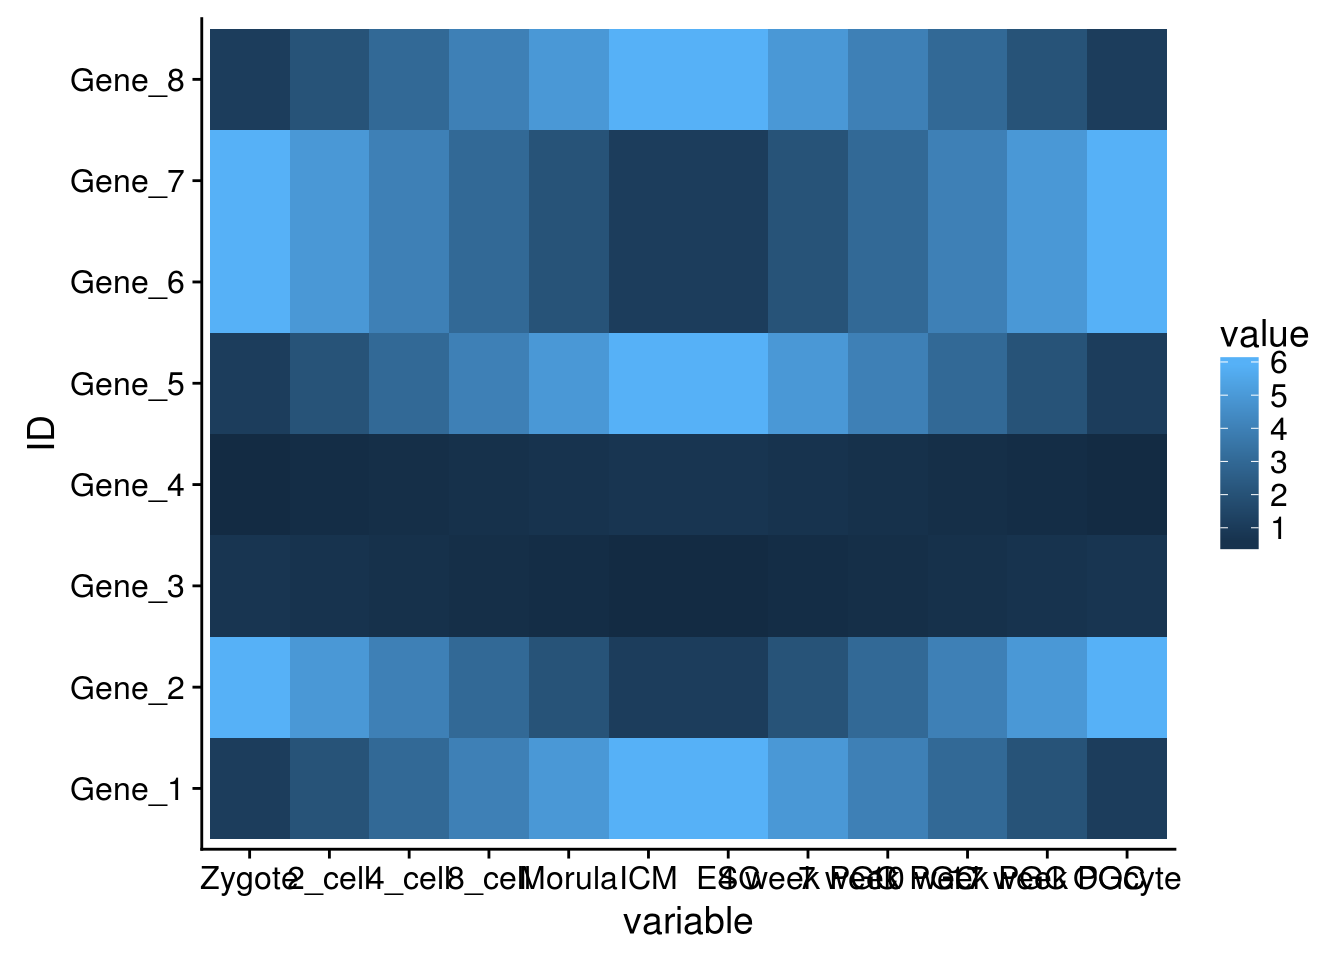
\includegraphics[width=0.95\linewidth,height=0.7\textheight,keepaspectratio]{R_course_files/figure-latex/unnamed-chunk-96-1} \end{center}

热图出来了,但有点不对劲,横轴重叠一起了。一个办法是调整图像的宽度,另一个是旋转横轴标记。

\begin{Shaded}
\begin{Highlighting}[]
\CommentTok{# theme: 是处理图美观的一个函数,可以调整横纵轴label的选择、图例的位置等。}
\CommentTok{# 这里选择X轴标签45度。}
\CommentTok{# hjust和vjust调整标签的相对位置,}
\CommentTok{# 具体见下图。}
\CommentTok{# 简单说,hjust是水平的对齐方式,0为左,1为右,0.5居中,0-1之间可以取任意值。}
\CommentTok{# vjust是垂直对齐方式,0底对齐,1为顶对齐,0.5居中,0-1之间可以取任意值。}

\NormalTok{p <-}\StringTok{ }\NormalTok{p +}\StringTok{ }\KeywordTok{theme}\NormalTok{(}\DataTypeTok{axis.text.x=}\KeywordTok{element_text}\NormalTok{(}\DataTypeTok{angle=}\DecValTok{45}\NormalTok{,}\DataTypeTok{hjust=}\DecValTok{1}\NormalTok{, }\DataTypeTok{vjust=}\DecValTok{1}\NormalTok{))}
\NormalTok{p}
\end{Highlighting}
\end{Shaded}

\begin{center}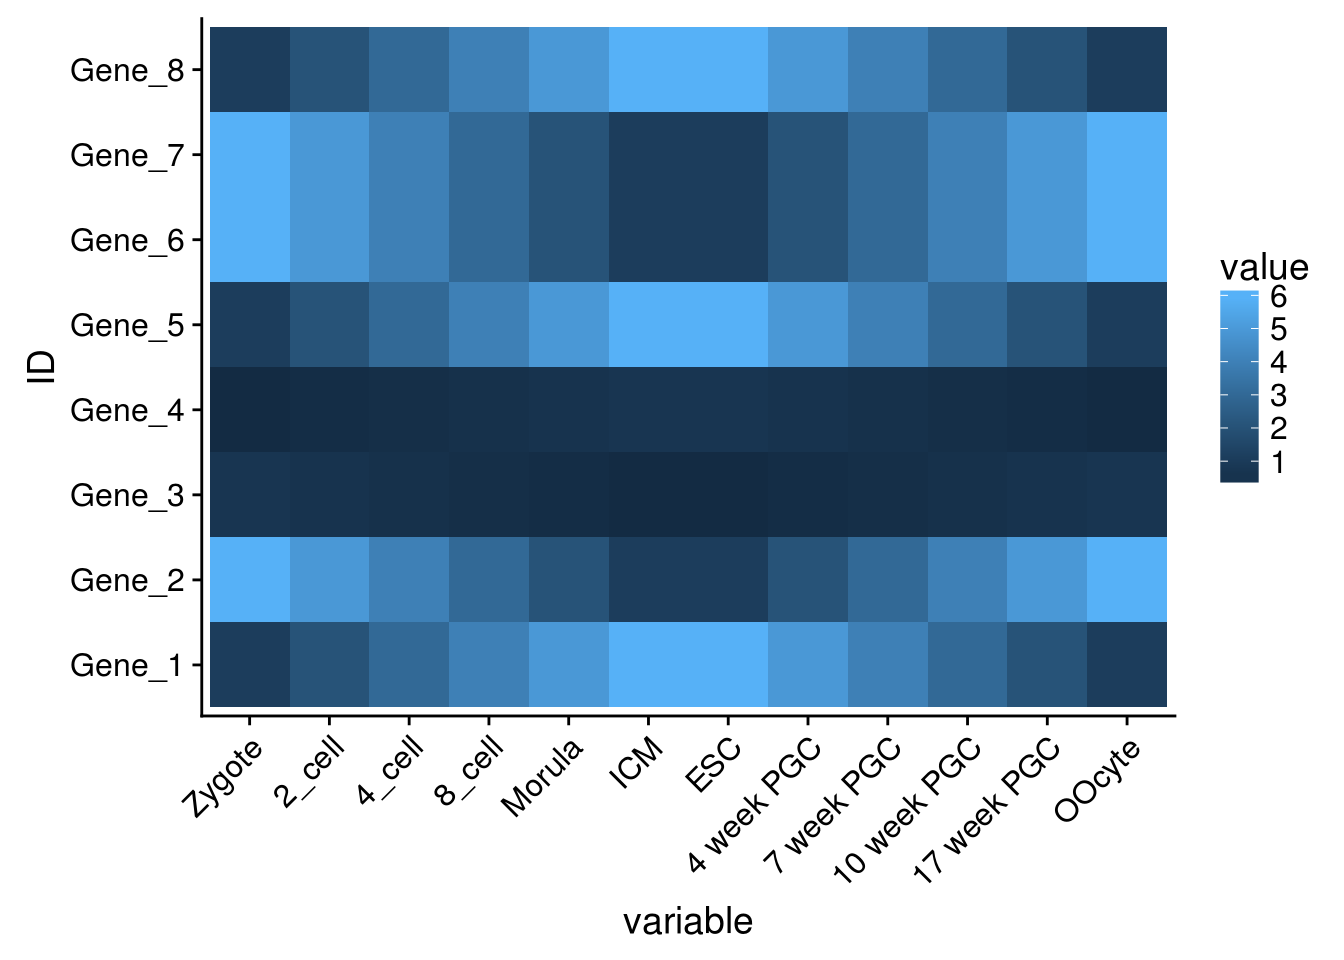
\includegraphics[width=0.95\linewidth,height=0.7\textheight,keepaspectratio]{R_course_files/figure-latex/unnamed-chunk-97-1} \end{center}

\begin{Shaded}
\begin{Highlighting}[]
\CommentTok{#knitr::include_graphics("images/hjust_vjust.png")}
\NormalTok{td <-}\StringTok{ }\KeywordTok{expand.grid}\NormalTok{(}
    \DataTypeTok{hjust=}\KeywordTok{c}\NormalTok{(}\DecValTok{0}\NormalTok{, }\FloatTok{0.5}\NormalTok{, }\DecValTok{1}\NormalTok{),}
    \DataTypeTok{vjust=}\KeywordTok{c}\NormalTok{(}\DecValTok{0}\NormalTok{, }\FloatTok{0.5}\NormalTok{, }\DecValTok{1}\NormalTok{),}
    \DataTypeTok{angle=}\KeywordTok{c}\NormalTok{(}\DecValTok{0}\NormalTok{, }\DecValTok{45}\NormalTok{, }\DecValTok{90}\NormalTok{),}
    \DataTypeTok{text=}\StringTok{"text"}
\NormalTok{)}

\KeywordTok{ggplot}\NormalTok{(td, }\KeywordTok{aes}\NormalTok{(}\DataTypeTok{x=}\NormalTok{hjust, }\DataTypeTok{y=}\NormalTok{vjust)) +}\StringTok{ }
\StringTok{    }\KeywordTok{geom_point}\NormalTok{() +}
\StringTok{    }\KeywordTok{geom_text}\NormalTok{(}\KeywordTok{aes}\NormalTok{(}\DataTypeTok{label=}\NormalTok{text, }\DataTypeTok{angle=}\NormalTok{angle, }\DataTypeTok{hjust=}\NormalTok{hjust, }\DataTypeTok{vjust=}\NormalTok{vjust)) +}\StringTok{ }
\StringTok{    }\KeywordTok{facet_grid}\NormalTok{(~angle) +}
\StringTok{    }\KeywordTok{scale_x_continuous}\NormalTok{(}\DataTypeTok{breaks=}\KeywordTok{c}\NormalTok{(}\DecValTok{0}\NormalTok{, }\FloatTok{0.5}\NormalTok{, }\DecValTok{1}\NormalTok{), }\DataTypeTok{expand=}\KeywordTok{c}\NormalTok{(}\DecValTok{0}\NormalTok{, }\FloatTok{0.2}\NormalTok{)) +}
\StringTok{    }\KeywordTok{scale_y_continuous}\NormalTok{(}\DataTypeTok{breaks=}\KeywordTok{c}\NormalTok{(}\DecValTok{0}\NormalTok{, }\FloatTok{0.5}\NormalTok{, }\DecValTok{1}\NormalTok{), }\DataTypeTok{expand=}\KeywordTok{c}\NormalTok{(}\DecValTok{0}\NormalTok{, }\FloatTok{0.2}\NormalTok{))}
\end{Highlighting}
\end{Shaded}

\begin{center}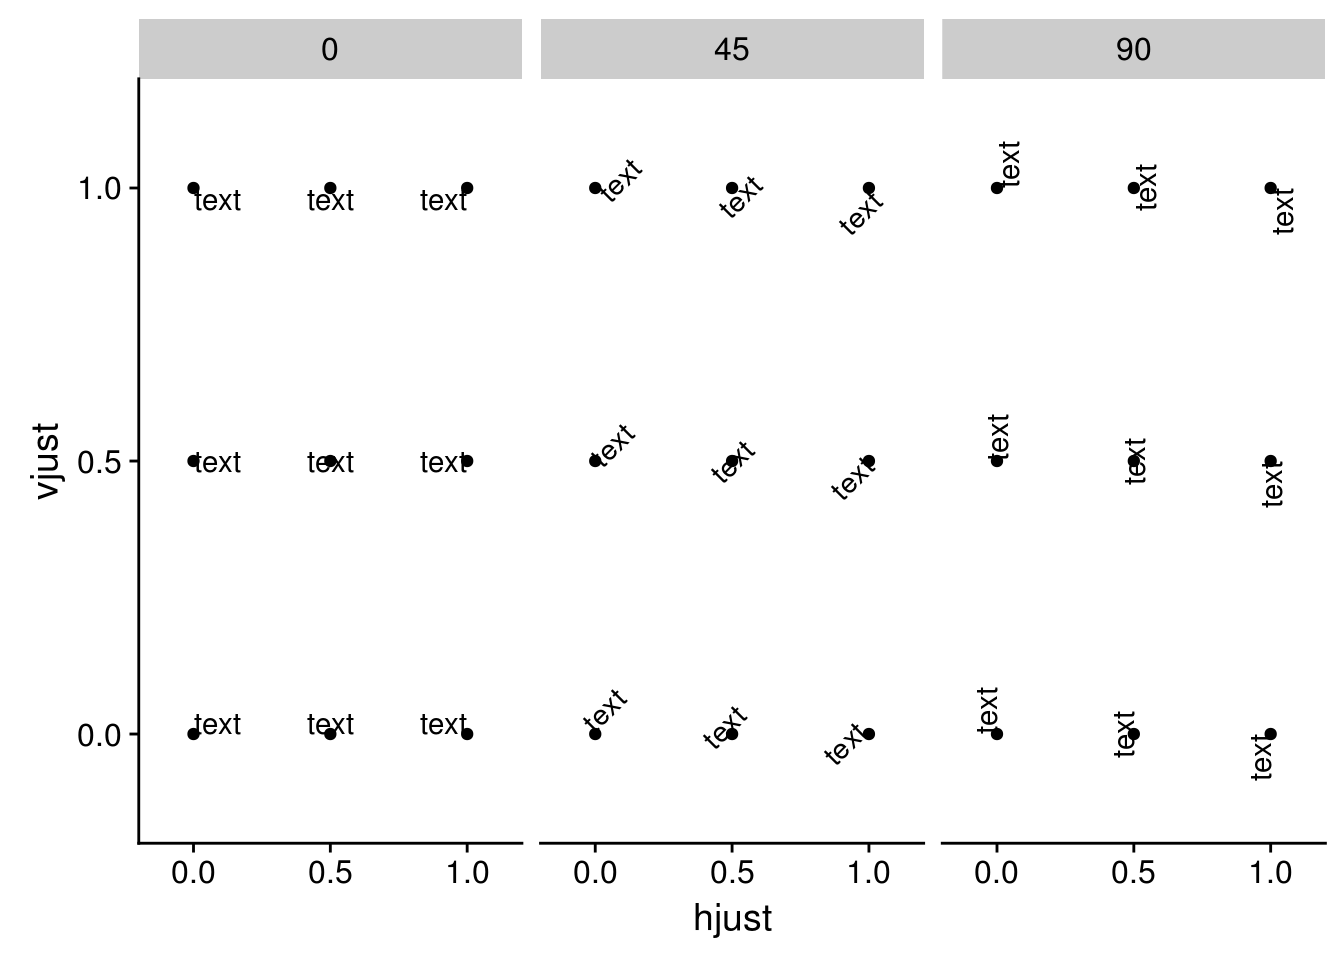
\includegraphics[width=0.95\linewidth,height=0.7\textheight,keepaspectratio]{R_course_files/figure-latex/unnamed-chunk-98-1} \end{center}

\url{http://stackoverflow.com/questions/7263849/what-do-hjust-and-vjust-do-when-making-a-plot-using-ggplot}

设置想要的颜色。

\begin{Shaded}
\begin{Highlighting}[]
\CommentTok{# 连续的数字,指定最小数值代表的颜色和最大数值赋予的颜色}
\CommentTok{# 注意fill和color的区别,fill是填充,color只针对边缘}
\NormalTok{p <-}\StringTok{ }\NormalTok{p +}\StringTok{ }\KeywordTok{scale_fill_gradient}\NormalTok{(}\DataTypeTok{low =} \StringTok{"white"}\NormalTok{, }\DataTypeTok{high =} \StringTok{"red"}\NormalTok{)}
\NormalTok{p}
\end{Highlighting}
\end{Shaded}

\begin{center}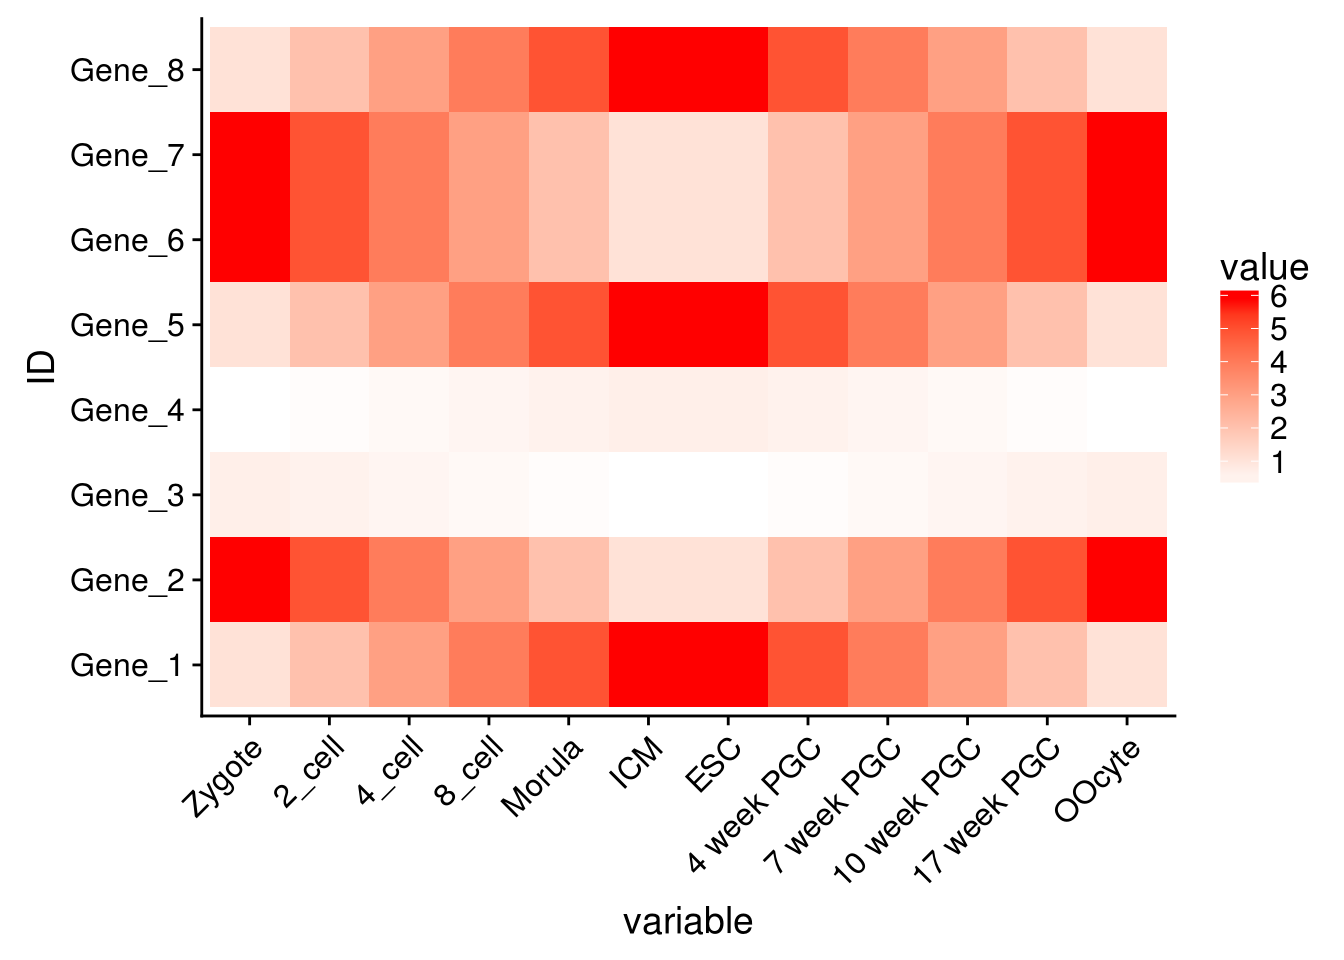
\includegraphics[width=0.95\linewidth,height=0.7\textheight,keepaspectratio]{R_course_files/figure-latex/unnamed-chunk-99-1} \end{center}

调整legend的位置, \texttt{legend.position}, 可以接受的值有 \texttt{top},
\texttt{bottom}, \texttt{left}, \texttt{right}, 和一个坐标
\texttt{c(0.05,0.8)}
(左上角,坐标是相对于图的左下角(即\textbf{原点})计算的)

\begin{Shaded}
\begin{Highlighting}[]
\NormalTok{p <-}\StringTok{ }\NormalTok{p +}\StringTok{ }\KeywordTok{theme}\NormalTok{(}\DataTypeTok{legend.position=}\StringTok{"top"}\NormalTok{)}
\NormalTok{p}
\end{Highlighting}
\end{Shaded}

\begin{center}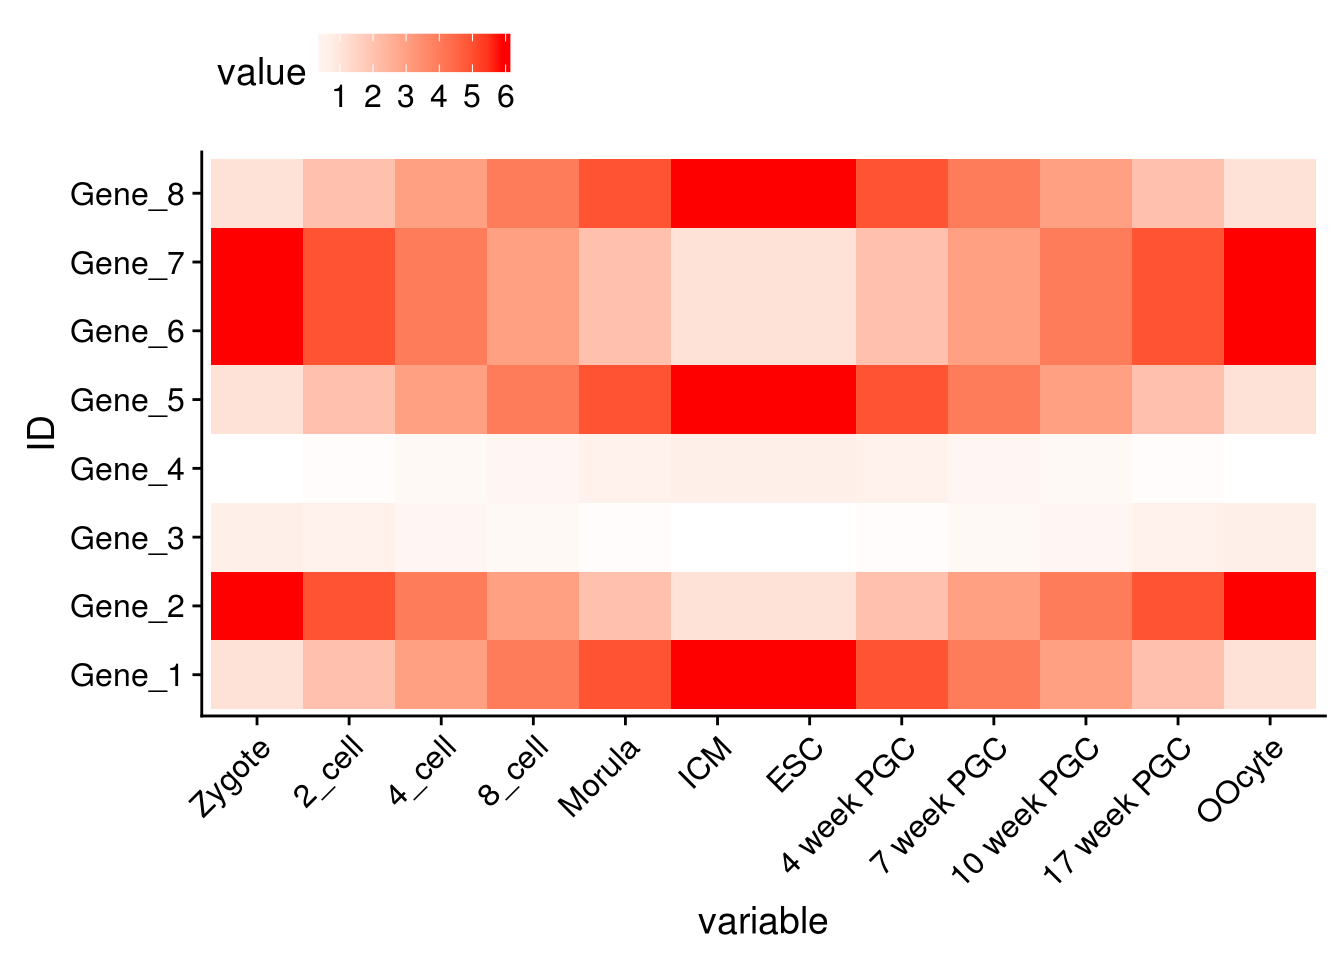
\includegraphics[width=0.95\linewidth,height=0.7\textheight,keepaspectratio]{R_course_files/figure-latex/unnamed-chunk-100-1} \end{center}

调整背景和背景格线以及X轴、Y轴的标题。

\begin{Shaded}
\begin{Highlighting}[]
\NormalTok{p <-}\StringTok{ }\NormalTok{p +}\StringTok{ }\KeywordTok{xlab}\NormalTok{(}\StringTok{"samples"}\NormalTok{) +}\StringTok{ }\KeywordTok{theme_bw}\NormalTok{() +}\StringTok{ }\KeywordTok{theme}\NormalTok{(}\DataTypeTok{panel.grid.major =} \KeywordTok{element_blank}\NormalTok{()) +}\StringTok{ }
\StringTok{    }\KeywordTok{theme}\NormalTok{(}\DataTypeTok{legend.key=}\KeywordTok{element_blank}\NormalTok{())}
\NormalTok{p}
\end{Highlighting}
\end{Shaded}

\begin{center}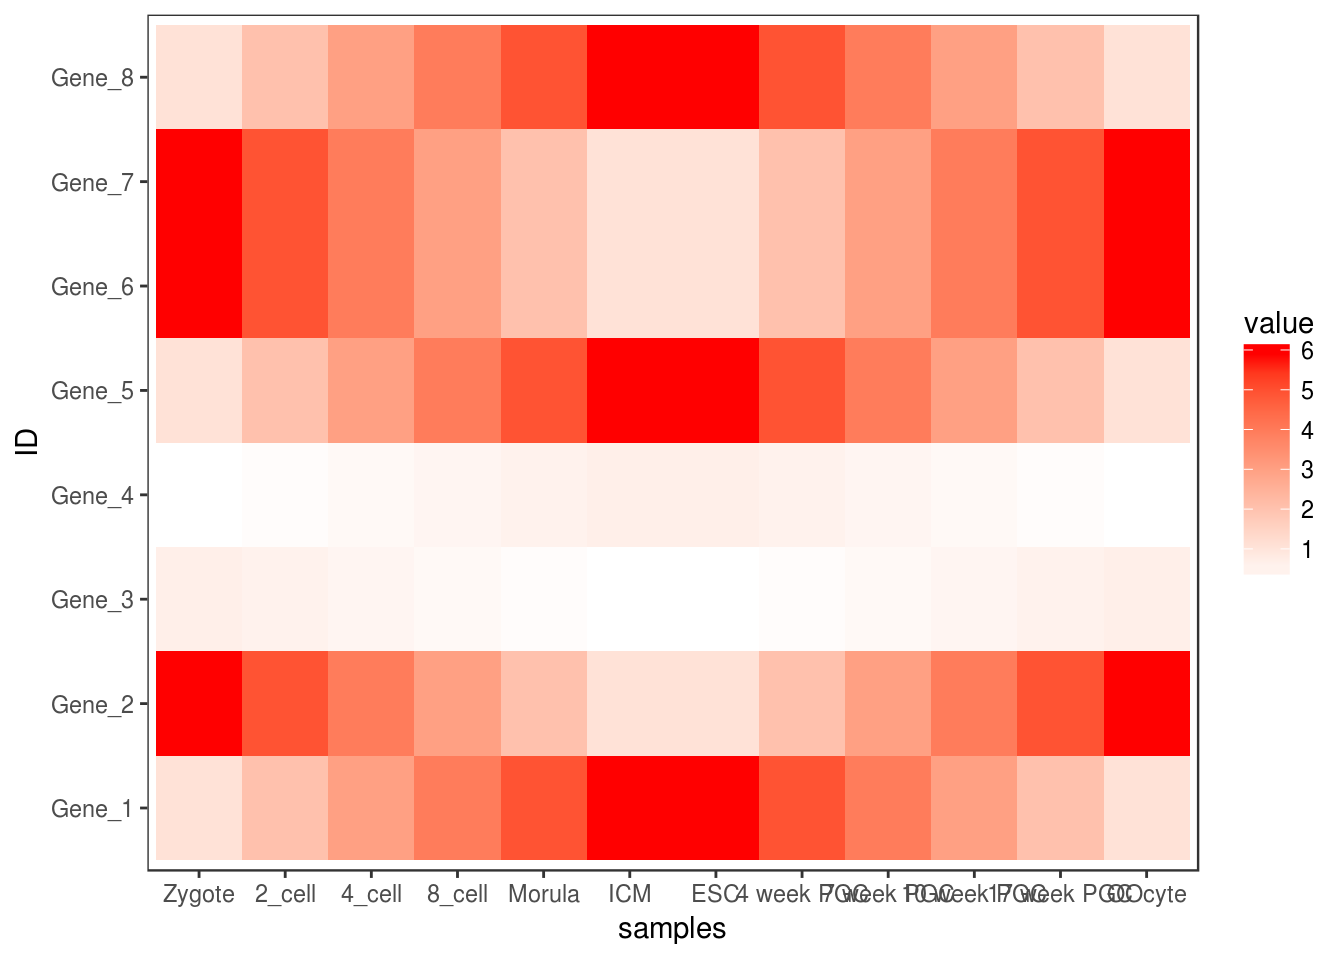
\includegraphics[width=0.95\linewidth,height=0.7\textheight,keepaspectratio]{R_course_files/figure-latex/unnamed-chunk-101-1} \end{center}

为了使横轴旋转45度,需要把这句话\texttt{theme(axis.text.x=element\_text(angle=45,hjust=1,\ vjust=1))}放在\texttt{theme\_bw()}的后面。

\begin{Shaded}
\begin{Highlighting}[]
\NormalTok{p <-}\StringTok{ }\NormalTok{p +}\StringTok{ }\KeywordTok{theme}\NormalTok{(}\DataTypeTok{axis.text.x=}\KeywordTok{element_text}\NormalTok{(}\DataTypeTok{angle=}\DecValTok{45}\NormalTok{,}\DataTypeTok{hjust=}\DecValTok{1}\NormalTok{, }\DataTypeTok{vjust=}\DecValTok{1}\NormalTok{))}
\NormalTok{p}
\end{Highlighting}
\end{Shaded}

\begin{center}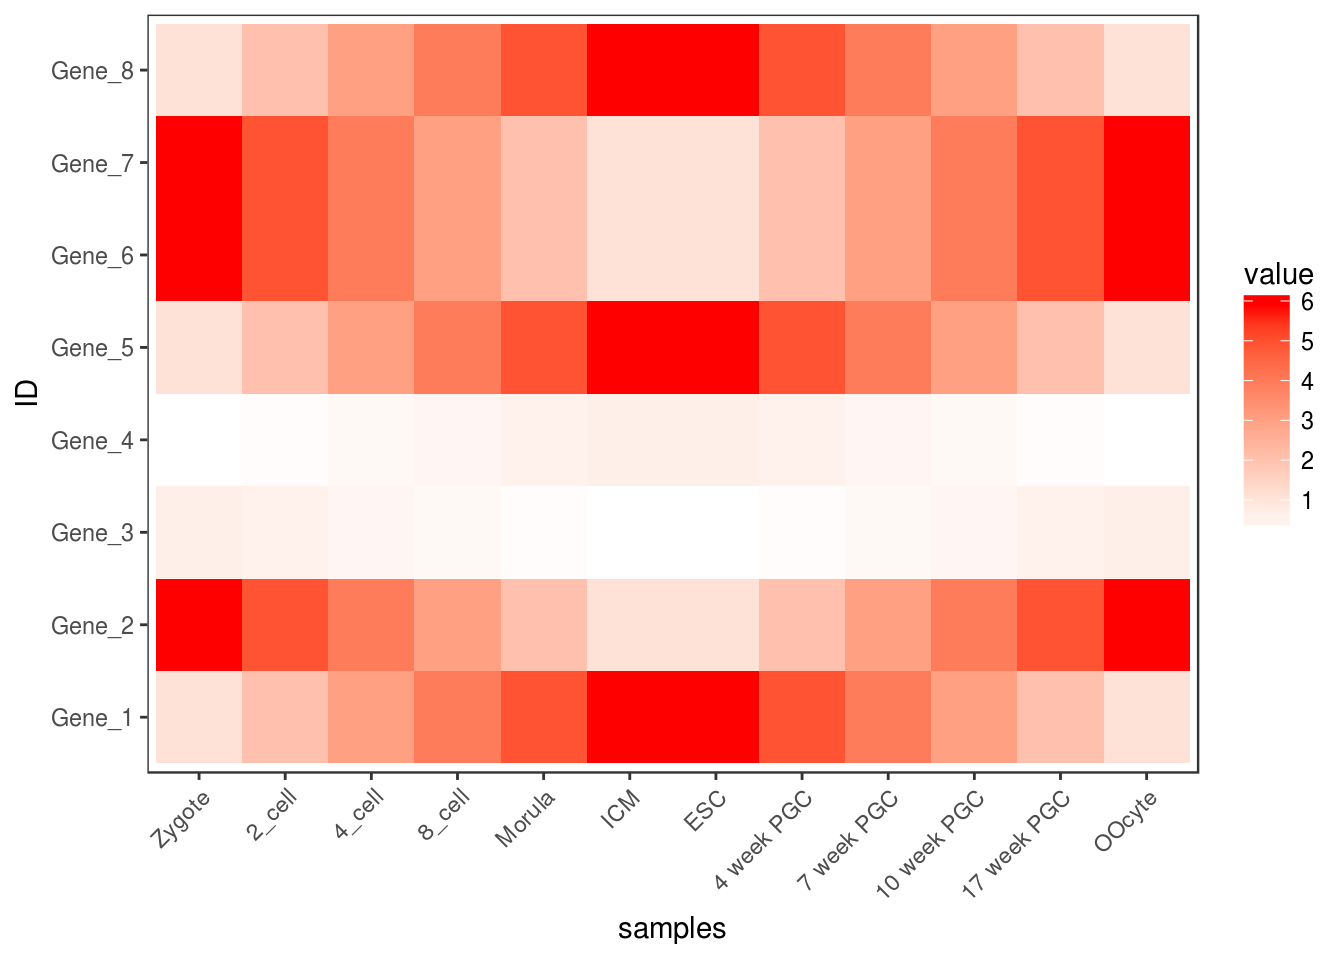
\includegraphics[width=0.95\linewidth,height=0.7\textheight,keepaspectratio]{R_course_files/figure-latex/unnamed-chunk-102-1} \end{center}

合并以上命令,就得到了下面这个看似复杂的绘图命令。

\begin{Shaded}
\begin{Highlighting}[]
\NormalTok{p <-}\StringTok{ }\KeywordTok{ggplot}\NormalTok{(data_m, }\KeywordTok{aes}\NormalTok{(}\DataTypeTok{x=}\NormalTok{variable,}\DataTypeTok{y=}\NormalTok{ID)) +}\StringTok{ }\KeywordTok{xlab}\NormalTok{(}\StringTok{"samples"}\NormalTok{) +}\StringTok{ }\KeywordTok{theme_bw}\NormalTok{() +}\StringTok{ }
\StringTok{    }\KeywordTok{theme}\NormalTok{(}\DataTypeTok{panel.grid.major =} \KeywordTok{element_blank}\NormalTok{()) +}\StringTok{ }\KeywordTok{theme}\NormalTok{(}\DataTypeTok{legend.key=}\KeywordTok{element_blank}\NormalTok{()) +}\StringTok{ }
\StringTok{    }\KeywordTok{theme}\NormalTok{(}\DataTypeTok{axis.text.x=}\KeywordTok{element_text}\NormalTok{(}\DataTypeTok{angle=}\DecValTok{45}\NormalTok{,}\DataTypeTok{hjust=}\DecValTok{1}\NormalTok{, }\DataTypeTok{vjust=}\DecValTok{1}\NormalTok{)) +}\StringTok{ }
\StringTok{    }\KeywordTok{theme}\NormalTok{(}\DataTypeTok{legend.position=}\StringTok{"top"}\NormalTok{) +}\StringTok{  }\KeywordTok{geom_tile}\NormalTok{(}\KeywordTok{aes}\NormalTok{(}\DataTypeTok{fill=}\NormalTok{value)) +}\StringTok{ }
\StringTok{    }\KeywordTok{scale_fill_gradient}\NormalTok{(}\DataTypeTok{low =} \StringTok{"white"}\NormalTok{, }\DataTypeTok{high =} \StringTok{"red"}\NormalTok{) +}
\StringTok{  }\KeywordTok{geom_point}\NormalTok{(}\KeywordTok{aes}\NormalTok{(}\DataTypeTok{color=}\NormalTok{value), }\DataTypeTok{size=}\DecValTok{6}\NormalTok{) +}
\StringTok{  }\KeywordTok{geom_text}\NormalTok{(}\KeywordTok{aes}\NormalTok{(}\DataTypeTok{label=}\NormalTok{value))}
\NormalTok{p}
\end{Highlighting}
\end{Shaded}

\begin{center}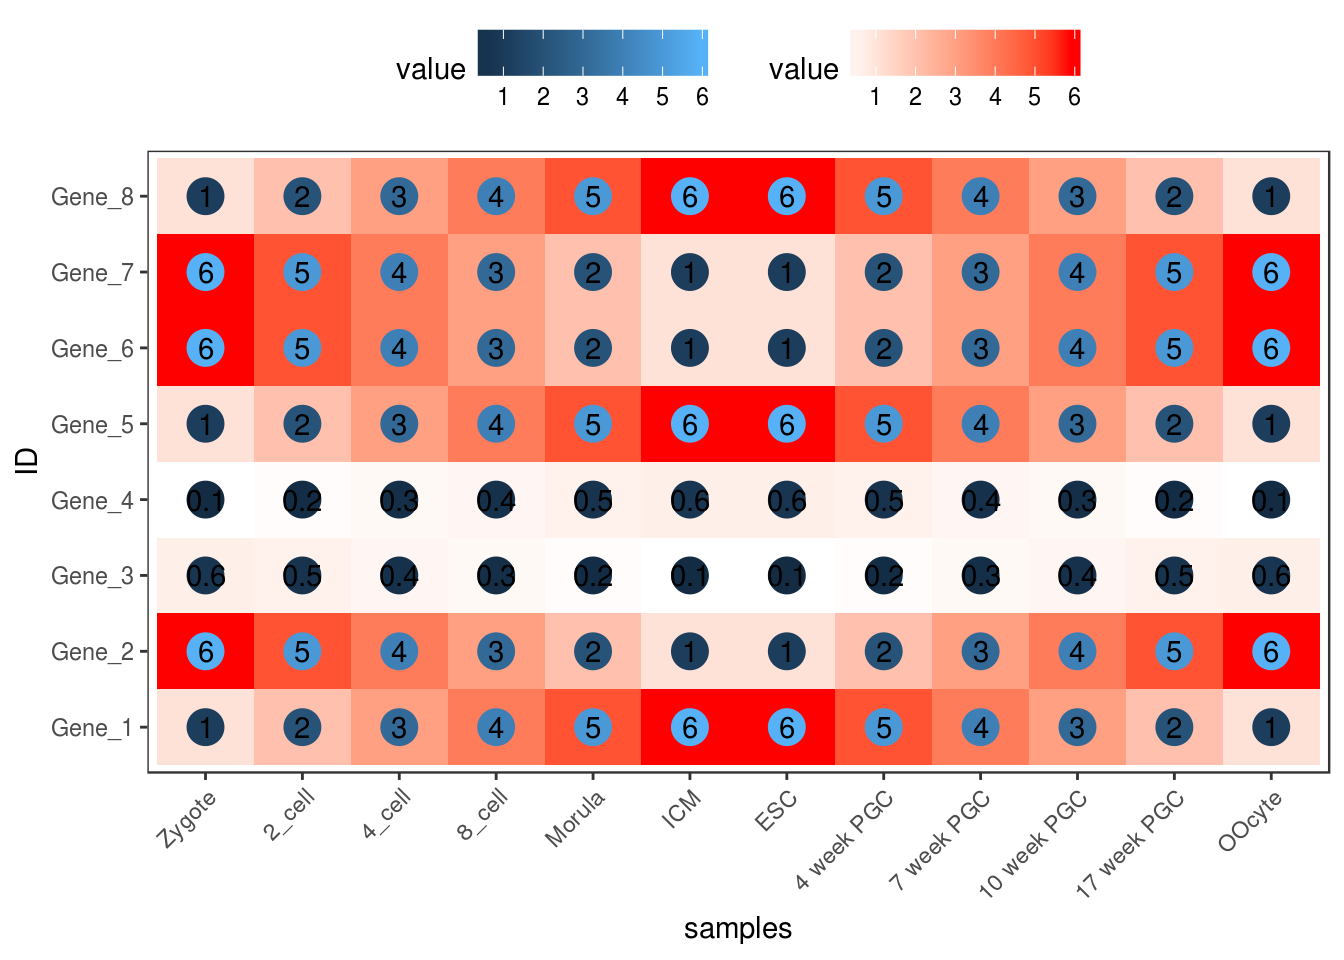
\includegraphics[width=0.95\linewidth,height=0.7\textheight,keepaspectratio]{R_course_files/figure-latex/unnamed-chunk-103-1} \end{center}

也可以只用Point

\begin{Shaded}
\begin{Highlighting}[]
\NormalTok{p <-}\StringTok{ }\KeywordTok{ggplot}\NormalTok{(data_m, }\KeywordTok{aes}\NormalTok{(}\DataTypeTok{x=}\NormalTok{variable,}\DataTypeTok{y=}\NormalTok{ID)) +}\StringTok{ }\KeywordTok{xlab}\NormalTok{(}\StringTok{"samples"}\NormalTok{) +}\StringTok{ }\KeywordTok{theme_bw}\NormalTok{() +}\StringTok{ }
\StringTok{    }\KeywordTok{theme}\NormalTok{(}\DataTypeTok{panel.grid.major =} \KeywordTok{element_blank}\NormalTok{()) +}\StringTok{ }\KeywordTok{theme}\NormalTok{(}\DataTypeTok{legend.key=}\KeywordTok{element_blank}\NormalTok{()) +}\StringTok{ }
\StringTok{    }\KeywordTok{theme}\NormalTok{(}\DataTypeTok{axis.text.x=}\KeywordTok{element_text}\NormalTok{(}\DataTypeTok{angle=}\DecValTok{45}\NormalTok{,}\DataTypeTok{hjust=}\DecValTok{1}\NormalTok{, }\DataTypeTok{vjust=}\DecValTok{1}\NormalTok{)) +}\StringTok{ }
\StringTok{    }\KeywordTok{theme}\NormalTok{(}\DataTypeTok{legend.position=}\StringTok{"top"}\NormalTok{) +}\StringTok{      }
\StringTok{  }\KeywordTok{geom_point}\NormalTok{(}\KeywordTok{aes}\NormalTok{(}\DataTypeTok{color=}\NormalTok{value), }\DataTypeTok{size=}\DecValTok{6}\NormalTok{) +}
\StringTok{  }\KeywordTok{scale_color_gradient}\NormalTok{(}\DataTypeTok{low =} \StringTok{"white"}\NormalTok{, }\DataTypeTok{high =} \StringTok{"red"}\NormalTok{) +}
\StringTok{  }\KeywordTok{geom_text}\NormalTok{(}\KeywordTok{aes}\NormalTok{(}\DataTypeTok{label=}\NormalTok{value))}
\NormalTok{p}
\end{Highlighting}
\end{Shaded}

\begin{center}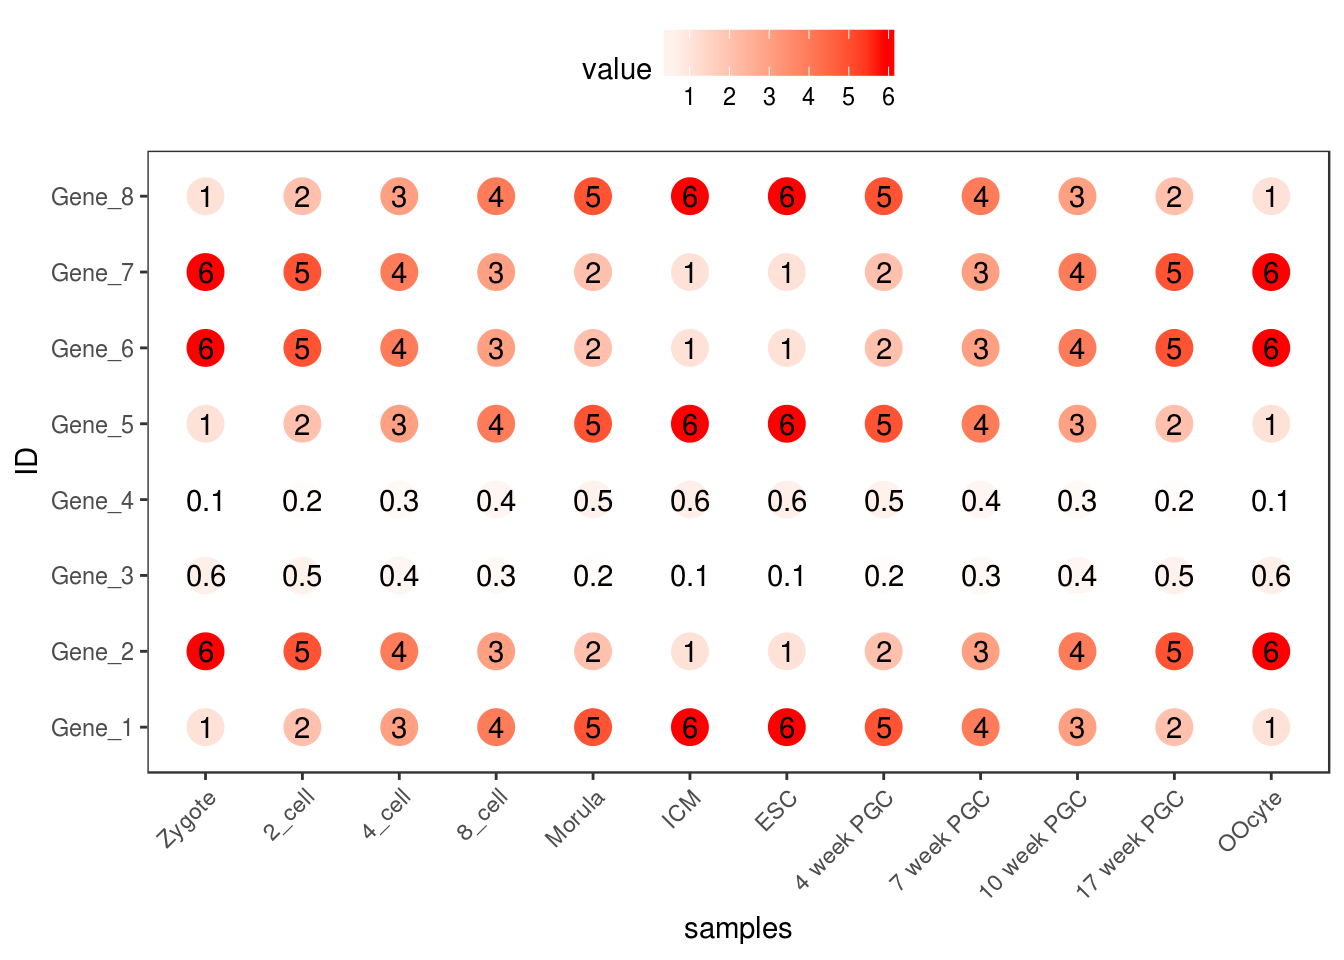
\includegraphics[width=0.95\linewidth,height=0.7\textheight,keepaspectratio]{R_course_files/figure-latex/unnamed-chunk-104-1} \end{center}

\subsubsection{图形存储}

图形出来了,就得考虑存储了,一般输出为\texttt{PDF}格式,方便后期的修改。

\begin{Shaded}
\begin{Highlighting}[]
\CommentTok{# 可以跟输出文件不同的后缀,以获得不同的输出格式}
\CommentTok{# colormode支持srgb (屏幕)和cmyk (打印,部分杂志需要,看上去有点褪色的感觉)格式}
\KeywordTok{ggsave}\NormalTok{(p, }\DataTypeTok{filename=}\StringTok{"heatmap.pdf"}\NormalTok{, }\DataTypeTok{width=}\DecValTok{10}\NormalTok{,}
        \DataTypeTok{height=}\DecValTok{15}\NormalTok{, }\DataTypeTok{units=}\KeywordTok{c}\NormalTok{(}\StringTok{"cm"}\NormalTok{),}\DataTypeTok{colormodel=}\StringTok{"srgb"}\NormalTok{)}
\end{Highlighting}
\end{Shaded}

点击下载:\href{heatmap.pdf}{pdf}

至此,完成了简单的heatmap的绘图。但实际绘制时,经常会碰到由于数值变化很大,导致颜色过于集中,使得图的可读性下降很多。因此需要对数据进行一些处理,具体的下次再说。

\subsection{热图美化}

上面的测试数据,数值的分布比较均一,相差不是太大,但是\texttt{Gene\_4}和\texttt{Gene\_5}由于整体的值低于其它的基因,从颜色上看,不仔细看,看不出差别。

\begin{Shaded}
\begin{Highlighting}[]
\NormalTok{data <-}\StringTok{ }\KeywordTok{c}\NormalTok{(}\KeywordTok{rnorm}\NormalTok{(}\DecValTok{5}\NormalTok{,}\DataTypeTok{mean=}\DecValTok{5}\NormalTok{), }\KeywordTok{rnorm}\NormalTok{(}\DecValTok{5}\NormalTok{,}\DataTypeTok{mean=}\DecValTok{20}\NormalTok{), }\KeywordTok{rnorm}\NormalTok{(}\DecValTok{5}\NormalTok{, }\DataTypeTok{mean=}\DecValTok{100}\NormalTok{), }\KeywordTok{c}\NormalTok{(}\DecValTok{600}\NormalTok{,}\DecValTok{700}\NormalTok{,}\DecValTok{800}\NormalTok{,}\DecValTok{900}\NormalTok{,}\DecValTok{10000}\NormalTok{))}
\NormalTok{data <-}\StringTok{ }\KeywordTok{matrix}\NormalTok{(data, }\DataTypeTok{ncol=}\DecValTok{5}\NormalTok{, }\DataTypeTok{byrow=}\NormalTok{T)}
\NormalTok{data <-}\StringTok{ }\KeywordTok{as.data.frame}\NormalTok{(data)}
\KeywordTok{rownames}\NormalTok{(data) <-}\StringTok{ }\NormalTok{letters[}\DecValTok{1}\NormalTok{:}\DecValTok{4}\NormalTok{]}
\KeywordTok{colnames}\NormalTok{(data) <-}\StringTok{ }\KeywordTok{paste}\NormalTok{(}\StringTok{"Grp"}\NormalTok{, }\DecValTok{1}\NormalTok{:}\DecValTok{5}\NormalTok{, }\DataTypeTok{sep=}\StringTok{"_"}\NormalTok{)}
\NormalTok{data}
\end{Highlighting}
\end{Shaded}

\begin{verbatim}
##        Grp_1      Grp_2      Grp_3      Grp_4        Grp_5
## a   6.087539   5.245061   7.075796   4.820246     4.374214
## b  18.391807  18.963660  20.210934  19.701757    21.620189
## c 100.005960  99.495593  99.766925  99.985531   100.411950
## d 600.000000 700.000000 800.000000 900.000000 10000.000000
\end{verbatim}

\begin{Shaded}
\begin{Highlighting}[]
\NormalTok{data$ID <-}\StringTok{ }\KeywordTok{rownames}\NormalTok{(data)}
\NormalTok{data}
\end{Highlighting}
\end{Shaded}

\begin{verbatim}
##        Grp_1      Grp_2      Grp_3      Grp_4        Grp_5 ID
## a   6.087539   5.245061   7.075796   4.820246     4.374214  a
## b  18.391807  18.963660  20.210934  19.701757    21.620189  b
## c 100.005960  99.495593  99.766925  99.985531   100.411950  c
## d 600.000000 700.000000 800.000000 900.000000 10000.000000  d
\end{verbatim}

\begin{Shaded}
\begin{Highlighting}[]
\NormalTok{data_m <-}\StringTok{ }\KeywordTok{melt}\NormalTok{(data, }\DataTypeTok{id.vars=}\KeywordTok{c}\NormalTok{(}\StringTok{"ID"}\NormalTok{))}
\KeywordTok{head}\NormalTok{(data_m)}
\end{Highlighting}
\end{Shaded}

\begin{verbatim}
##   ID variable      value
## 1  a    Grp_1   6.087539
## 2  b    Grp_1  18.391807
## 3  c    Grp_1 100.005960
## 4  d    Grp_1 600.000000
## 5  a    Grp_2   5.245061
## 6  b    Grp_2  18.963660
\end{verbatim}

\begin{Shaded}
\begin{Highlighting}[]
\NormalTok{p <-}\StringTok{ }\KeywordTok{ggplot}\NormalTok{(data_m, }\KeywordTok{aes}\NormalTok{(}\DataTypeTok{x=}\NormalTok{variable,}\DataTypeTok{y=}\NormalTok{ID)) +}\StringTok{ }\KeywordTok{xlab}\NormalTok{(}\StringTok{"samples"}\NormalTok{) +}\StringTok{ }\KeywordTok{theme_bw}\NormalTok{() +}\StringTok{ }
\StringTok{    }\KeywordTok{theme}\NormalTok{(}\DataTypeTok{panel.grid.major =} \KeywordTok{element_blank}\NormalTok{()) +}\StringTok{ }\KeywordTok{theme}\NormalTok{(}\DataTypeTok{legend.key=}\KeywordTok{element_blank}\NormalTok{()) +}\StringTok{ }
\StringTok{    }\KeywordTok{theme}\NormalTok{(}\DataTypeTok{axis.text.x=}\KeywordTok{element_text}\NormalTok{(}\DataTypeTok{angle=}\DecValTok{45}\NormalTok{,}\DataTypeTok{hjust=}\DecValTok{1}\NormalTok{, }\DataTypeTok{vjust=}\DecValTok{1}\NormalTok{)) +}\StringTok{ }
\StringTok{    }\KeywordTok{theme}\NormalTok{(}\DataTypeTok{legend.position=}\StringTok{"top"}\NormalTok{) +}\StringTok{  }\KeywordTok{geom_tile}\NormalTok{(}\KeywordTok{aes}\NormalTok{(}\DataTypeTok{fill=}\NormalTok{value)) +}\StringTok{ }
\StringTok{    }\KeywordTok{scale_fill_gradient}\NormalTok{(}\DataTypeTok{low =} \StringTok{"white"}\NormalTok{, }\DataTypeTok{high =} \StringTok{"red"}\NormalTok{)}
\NormalTok{p}
\CommentTok{#dev.off()}
\end{Highlighting}
\end{Shaded}

\begin{center}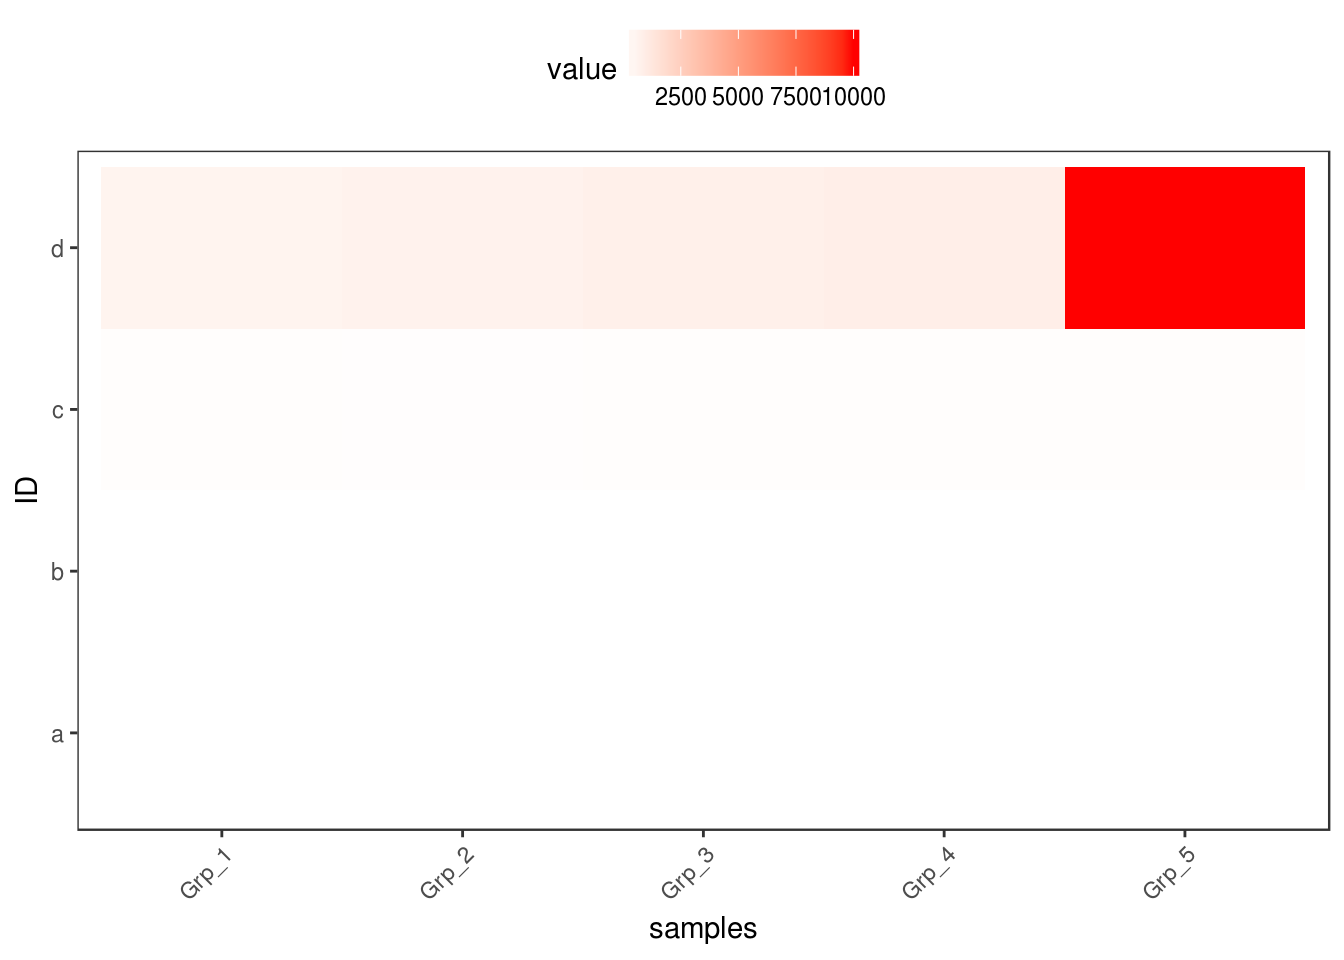
\includegraphics[width=0.95\linewidth,height=0.7\textheight,keepaspectratio]{R_course_files/figure-latex/unnamed-chunk-109-1} \end{center}

图中只有右上角可以看到红色,其他地方就没了颜色的差异。这通常不是我们想要的。为了更好的可视化效果,需要对数据做些预处理,主要有
\texttt{对数转换},\texttt{Z-score转换},\texttt{抹去异常值},\texttt{非线性颜色}等方式。

\subsubsection{对数转换}

假设下面的数据是基因表达数据,4个基因 (a, b, c, d)和5个样品 (Grp\_1,
Grp\_2, Grp\_3, Grp\_4),矩阵中的值代表基因表达FPKM值。

\begin{Shaded}
\begin{Highlighting}[]
\NormalTok{data <-}\StringTok{ }\KeywordTok{c}\NormalTok{(}\KeywordTok{rnorm}\NormalTok{(}\DecValTok{5}\NormalTok{,}\DataTypeTok{mean=}\DecValTok{5}\NormalTok{), }\KeywordTok{rnorm}\NormalTok{(}\DecValTok{5}\NormalTok{,}\DataTypeTok{mean=}\DecValTok{20}\NormalTok{), }\KeywordTok{rnorm}\NormalTok{(}\DecValTok{5}\NormalTok{, }\DataTypeTok{mean=}\DecValTok{100}\NormalTok{), }\KeywordTok{c}\NormalTok{(}\DecValTok{600}\NormalTok{,}\DecValTok{700}\NormalTok{,}\DecValTok{800}\NormalTok{,}\DecValTok{900}\NormalTok{,}\DecValTok{10000}\NormalTok{))}
\NormalTok{data <-}\StringTok{ }\KeywordTok{matrix}\NormalTok{(data, }\DataTypeTok{ncol=}\DecValTok{5}\NormalTok{, }\DataTypeTok{byrow=}\NormalTok{T)}
\NormalTok{data <-}\StringTok{ }\KeywordTok{as.data.frame}\NormalTok{(data)}
\KeywordTok{rownames}\NormalTok{(data) <-}\StringTok{ }\NormalTok{letters[}\DecValTok{1}\NormalTok{:}\DecValTok{4}\NormalTok{]}
\KeywordTok{colnames}\NormalTok{(data) <-}\StringTok{ }\KeywordTok{paste}\NormalTok{(}\StringTok{"Grp"}\NormalTok{, }\DecValTok{1}\NormalTok{:}\DecValTok{5}\NormalTok{, }\DataTypeTok{sep=}\StringTok{"_"}\NormalTok{)}
\NormalTok{data}
\end{Highlighting}
\end{Shaded}

\begin{verbatim}
##        Grp_1      Grp_2     Grp_3      Grp_4        Grp_5
## a   4.125538   4.087054   3.52572   5.749561     2.420971
## b  21.296682  19.922518  19.41533  20.510619    20.319078
## c 100.188919  99.774166  99.88726  98.414636   100.442783
## d 600.000000 700.000000 800.00000 900.000000 10000.000000
\end{verbatim}

\begin{Shaded}
\begin{Highlighting}[]
\NormalTok{data_log <-}\StringTok{ }\KeywordTok{log2}\NormalTok{(data}\DecValTok{+1}\NormalTok{)}
\NormalTok{data_log}
\end{Highlighting}
\end{Shaded}

\begin{verbatim}
##      Grp_1    Grp_2    Grp_3    Grp_4     Grp_5
## a 2.357704 2.346830 2.178147 2.754794  1.774406
## b 4.478757 4.386985 4.351581 4.426977  4.414073
## c 6.660907 6.654982 6.656600 6.635386  6.664522
## d 9.231221 9.453271 9.645658 9.815383 13.287857
\end{verbatim}

\begin{Shaded}
\begin{Highlighting}[]
\NormalTok{data_log$ID =}\StringTok{ }\KeywordTok{rownames}\NormalTok{(data_log)}
\NormalTok{data_log_m =}\StringTok{ }\KeywordTok{melt}\NormalTok{(data_log, }\DataTypeTok{id.vars=}\KeywordTok{c}\NormalTok{(}\StringTok{"ID"}\NormalTok{))}

\NormalTok{p <-}\StringTok{ }\KeywordTok{ggplot}\NormalTok{(data_log_m, }\KeywordTok{aes}\NormalTok{(}\DataTypeTok{x=}\NormalTok{variable,}\DataTypeTok{y=}\NormalTok{ID)) +}\StringTok{ }\KeywordTok{xlab}\NormalTok{(}\StringTok{"samples"}\NormalTok{) +}\StringTok{ }\KeywordTok{ylab}\NormalTok{(}\OtherTok{NULL}\NormalTok{) +}\StringTok{ }
\StringTok{    }\KeywordTok{theme_bw}\NormalTok{() +}\StringTok{ }\KeywordTok{theme}\NormalTok{(}\DataTypeTok{panel.grid.major =} \KeywordTok{element_blank}\NormalTok{()) +}\StringTok{ }
\StringTok{    }\KeywordTok{theme}\NormalTok{(}\DataTypeTok{legend.key=}\KeywordTok{element_blank}\NormalTok{()) +}\StringTok{ }\KeywordTok{theme}\NormalTok{(}\DataTypeTok{legend.position=}\StringTok{"top"}\NormalTok{) +}
\StringTok{    }\KeywordTok{theme}\NormalTok{(}\DataTypeTok{axis.text.x=}\KeywordTok{element_text}\NormalTok{(}\DataTypeTok{angle=}\DecValTok{45}\NormalTok{,}\DataTypeTok{hjust=}\DecValTok{1}\NormalTok{,}\DataTypeTok{vjust=}\DecValTok{1}\NormalTok{)) +}\StringTok{ }
\StringTok{    }\KeywordTok{geom_tile}\NormalTok{(}\KeywordTok{aes}\NormalTok{(}\DataTypeTok{fill=}\NormalTok{value)) +}\StringTok{ }\KeywordTok{scale_fill_gradient}\NormalTok{(}\DataTypeTok{low =} \StringTok{"white"}\NormalTok{, }\DataTypeTok{high =} \StringTok{"red"}\NormalTok{)}
\NormalTok{p}
\CommentTok{#ggsave(p, filename="heatmap_log.pdf", width=8, height=12, units=c("cm"),colormodel="srgb")}
\end{Highlighting}
\end{Shaded}

\begin{center}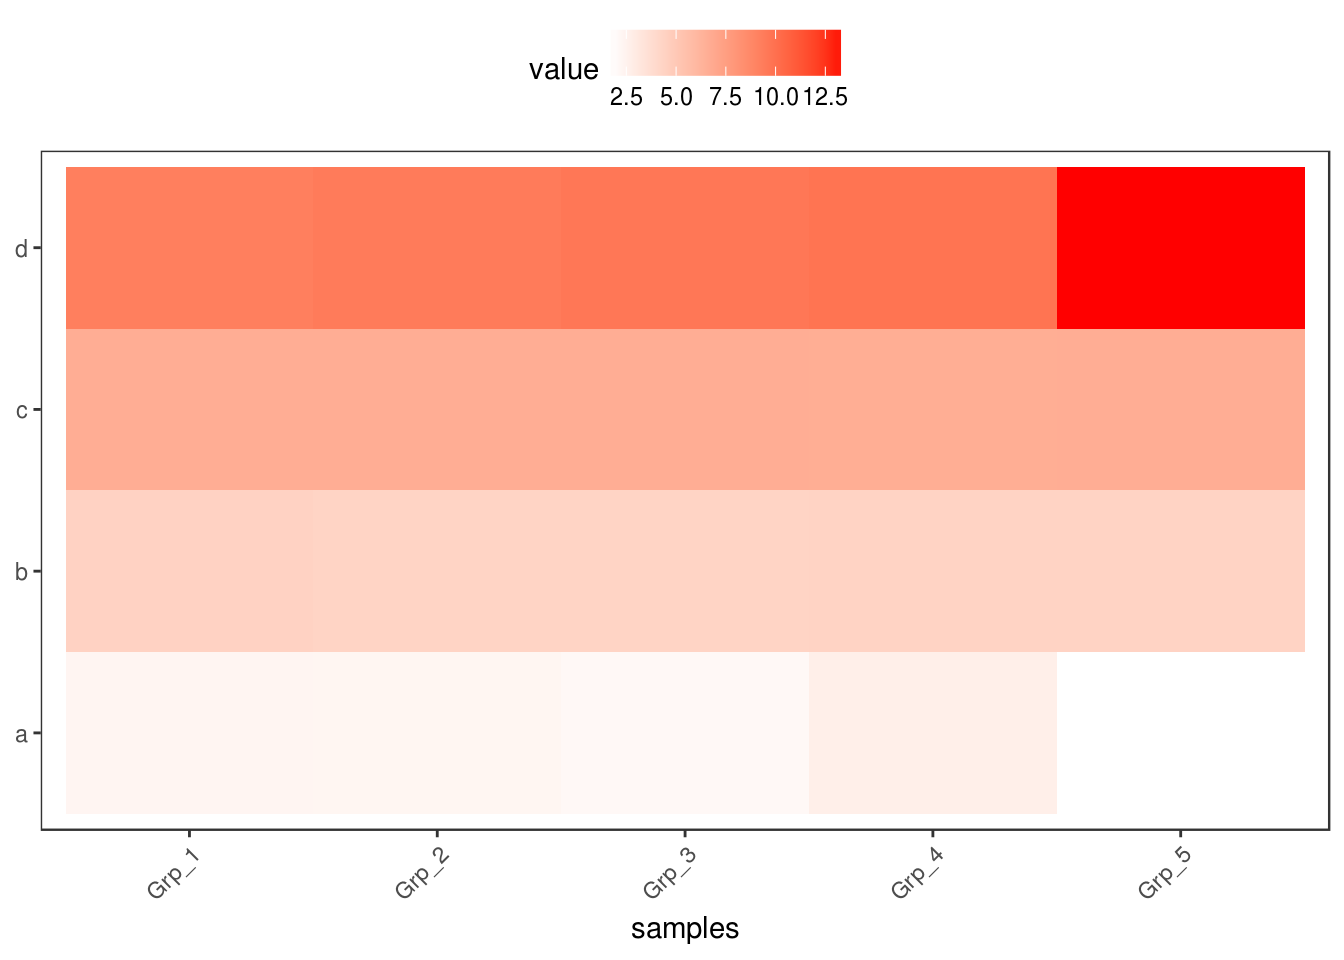
\includegraphics[width=0.95\linewidth,height=0.7\textheight,keepaspectratio]{R_course_files/figure-latex/unnamed-chunk-112-1} \end{center}

对数转换后的数据,看起来就清晰的多了。而且对数转换后,数据还保留着之前的变化趋势,不只是基因在不同样品之间的表达可比
(同一行的不同列),不同基因在同一样品的值也可比 (同一列的不同行)
(不同基因之间比较表达值存在理论上的问题,即便是按照长度标准化之后的FPKM也不代表基因之间是完全可比的)。

\subsubsection{Z-score转换}\label{z-score}

\texttt{Z-score}又称为标准分数,是一组数中的每个数减去这一组数的平均值再除以这一组数的标准差,代表的是原始分数距离原始平均值的距离,以标准差为单位。可以对不同分布的各原始分数进行比较,用来反映数据的相对变化趋势,而非绝对变化量。

\begin{Shaded}
\begin{Highlighting}[]
\NormalTok{data_ori <-}\StringTok{ "Grp_1;Grp_2;Grp_3;Grp_4;Grp_5}
\StringTok{a;6.6;20.9;100.1;600.0;5.2}
\StringTok{b;20.8;99.8;700.0;3.7;19.2}
\StringTok{c;100.0;800.0;6.2;21.4;98.6}
\StringTok{d;900;3.3;20.3;101.1;10000"}

\NormalTok{data <-}\StringTok{ }\KeywordTok{read.table}\NormalTok{(}\DataTypeTok{text=}\NormalTok{data_ori, }\DataTypeTok{header=}\NormalTok{T, }\DataTypeTok{row.names=}\DecValTok{1}\NormalTok{, }\DataTypeTok{sep=}\StringTok{";"}\NormalTok{, }\DataTypeTok{quote=}\StringTok{""}\NormalTok{)}

\CommentTok{# 去掉方差为0的行,也就是值全都一致的行}
\NormalTok{data <-}\StringTok{ }\NormalTok{data[}\KeywordTok{apply}\NormalTok{(data,}\DecValTok{1}\NormalTok{,var)!=}\DecValTok{0}\NormalTok{,]}

\NormalTok{data}
\end{Highlighting}
\end{Shaded}

\begin{verbatim}
##   Grp_1 Grp_2 Grp_3 Grp_4   Grp_5
## a   6.6  20.9 100.1 600.0     5.2
## b  20.8  99.8 700.0   3.7    19.2
## c 100.0 800.0   6.2  21.4    98.6
## d 900.0   3.3  20.3 101.1 10000.0
\end{verbatim}

\begin{Shaded}
\begin{Highlighting}[]
\CommentTok{# 标准化数据,并转换为data.frame}
\NormalTok{data_scale <-}\StringTok{ }\KeywordTok{as.data.frame}\NormalTok{(}\KeywordTok{t}\NormalTok{(}\KeywordTok{apply}\NormalTok{(data,}\DecValTok{1}\NormalTok{,scale)))}

\CommentTok{# 重命名列}
\KeywordTok{colnames}\NormalTok{(data_scale) <-}\StringTok{ }\KeywordTok{colnames}\NormalTok{(data)}
\NormalTok{data_scale}
\end{Highlighting}
\end{Shaded}

\begin{verbatim}
##        Grp_1      Grp_2      Grp_3      Grp_4      Grp_5
## a -0.5456953 -0.4899405 -0.1811446  1.7679341 -0.5511538
## b -0.4940465 -0.2301542  1.7747592 -0.5511674 -0.4993911
## c -0.3139042  1.7740182 -0.5936858 -0.5483481 -0.3180801
## d -0.2983707 -0.5033986 -0.4995116 -0.4810369  1.7823177
\end{verbatim}

\begin{Shaded}
\begin{Highlighting}[]
\NormalTok{data_scale$ID =}\StringTok{ }\KeywordTok{rownames}\NormalTok{(data_scale)}
\NormalTok{data_scale_m =}\StringTok{ }\KeywordTok{melt}\NormalTok{(data_scale, }\DataTypeTok{id.vars=}\KeywordTok{c}\NormalTok{(}\StringTok{"ID"}\NormalTok{))}
\NormalTok{data_scale_m$value <-}\StringTok{ }\KeywordTok{as.numeric}\NormalTok{(}\KeywordTok{prettyNum}\NormalTok{(data_scale_m$value, }\DataTypeTok{digits=}\DecValTok{2}\NormalTok{))}
\NormalTok{p <-}\StringTok{ }\KeywordTok{ggplot}\NormalTok{(data_scale_m, }\KeywordTok{aes}\NormalTok{(}\DataTypeTok{x=}\NormalTok{variable,}\DataTypeTok{y=}\NormalTok{ID)) +}\StringTok{ }\KeywordTok{xlab}\NormalTok{(}\StringTok{"samples"}\NormalTok{) +}\StringTok{ }\KeywordTok{ylab}\NormalTok{(}\OtherTok{NULL}\NormalTok{) +}\StringTok{ }
\StringTok{    }\KeywordTok{theme_bw}\NormalTok{() +}\StringTok{ }\KeywordTok{theme}\NormalTok{(}\DataTypeTok{panel.grid.major =} \KeywordTok{element_blank}\NormalTok{()) +}\StringTok{ }
\StringTok{    }\KeywordTok{theme}\NormalTok{(}\DataTypeTok{legend.key=}\KeywordTok{element_blank}\NormalTok{()) +}\StringTok{ }
\StringTok{    }\KeywordTok{theme}\NormalTok{(}\DataTypeTok{axis.text.x=}\KeywordTok{element_text}\NormalTok{(}\DataTypeTok{angle=}\DecValTok{45}\NormalTok{,}\DataTypeTok{hjust=}\DecValTok{1}\NormalTok{, }\DataTypeTok{vjust=}\DecValTok{1}\NormalTok{)) +}\StringTok{ }
\StringTok{    }\KeywordTok{geom_tile}\NormalTok{(}\KeywordTok{aes}\NormalTok{(}\DataTypeTok{fill=}\NormalTok{value)) +}\StringTok{ }\KeywordTok{scale_fill_gradient}\NormalTok{(}\DataTypeTok{low =} \StringTok{"white"}\NormalTok{, }\DataTypeTok{high =} \StringTok{"red"}\NormalTok{) +}
\StringTok{  }\KeywordTok{geom_text}\NormalTok{(}\KeywordTok{aes}\NormalTok{(}\DataTypeTok{label=}\NormalTok{value))}
\NormalTok{p}
\CommentTok{#ggsave(p, filename="heatmap_scale.pdf", width=8, height=12, units=c("cm"), }
\CommentTok{#    colormodel="srgb")}
\end{Highlighting}
\end{Shaded}

\begin{center}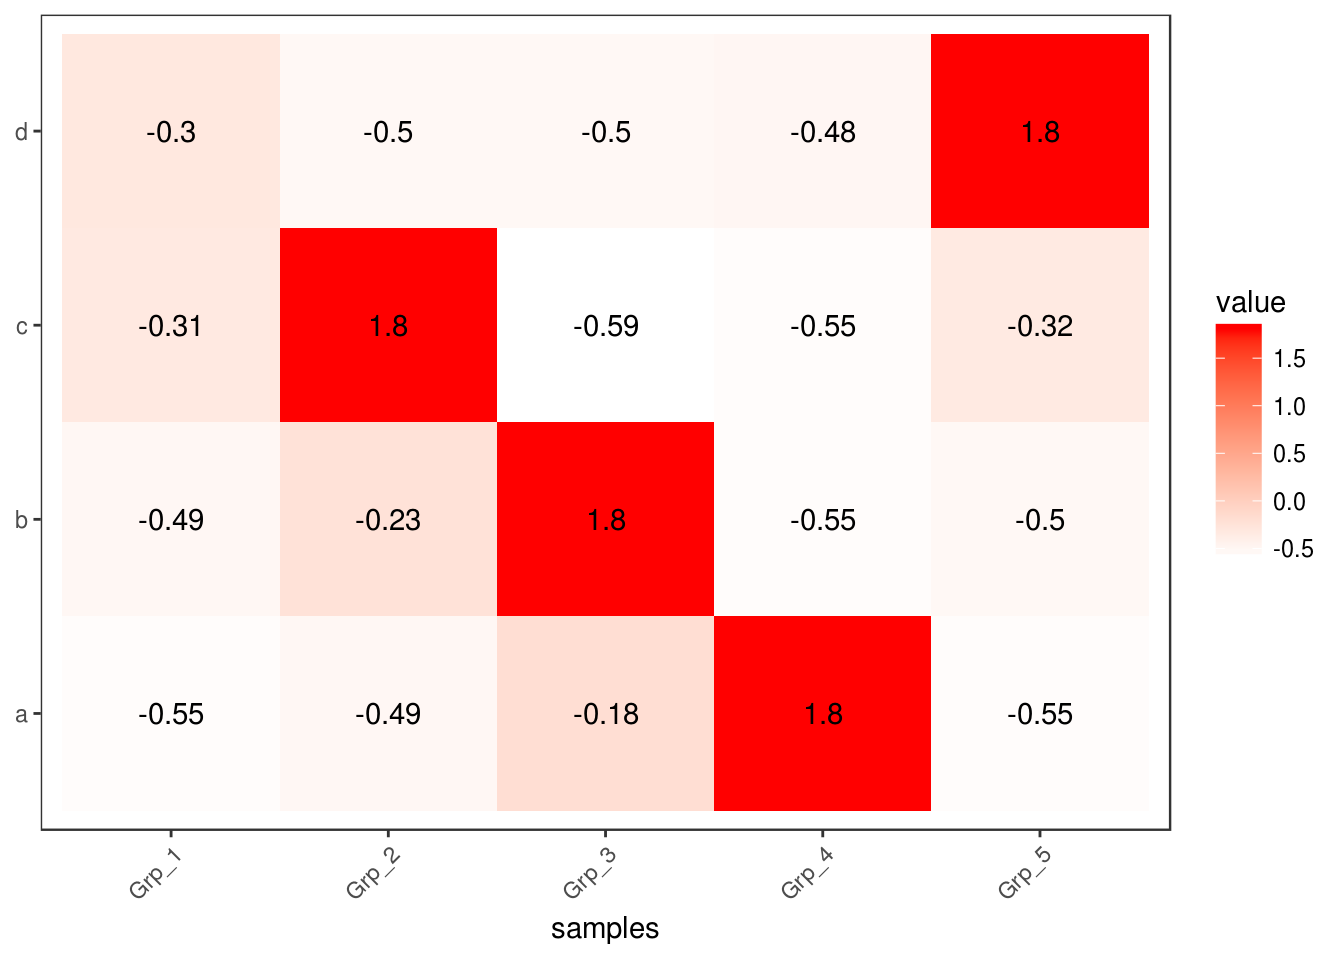
\includegraphics[width=0.95\linewidth,height=0.7\textheight,keepaspectratio]{R_course_files/figure-latex/unnamed-chunk-115-1} \end{center}

\texttt{Z-score}转换后,颜色分布也相对均一了,每个基因在不同样品之间的表达的高低一目了然。但是不同基因之间就完全不可比了。

\subsubsection{抹去异常值}

粗暴一点,假设检测饱和度为100,大于100的值都视为100对待。

\begin{Shaded}
\begin{Highlighting}[]
\NormalTok{data_ori <-}\StringTok{ "Grp_1;Grp_2;Grp_3;Grp_4;Grp_5}
\StringTok{a;6.6;20.9;100.1;600.0;5.2}
\StringTok{b;20.8;99.8;700.0;3.7;19.2}
\StringTok{c;100.0;800.0;6.2;21.4;98.6}
\StringTok{d;900;3.3;20.3;101.1;10000"}

\NormalTok{data <-}\StringTok{ }\KeywordTok{read.table}\NormalTok{(}\DataTypeTok{text=}\NormalTok{data_ori, }\DataTypeTok{header=}\NormalTok{T, }\DataTypeTok{row.names=}\DecValTok{1}\NormalTok{, }\DataTypeTok{sep=}\StringTok{";"}\NormalTok{, }\DataTypeTok{quote=}\StringTok{""}\NormalTok{)}

\NormalTok{data[data>}\DecValTok{100}\NormalTok{] <-}\StringTok{ }\DecValTok{100}
\NormalTok{data}
\end{Highlighting}
\end{Shaded}

\begin{verbatim}
##   Grp_1 Grp_2 Grp_3 Grp_4 Grp_5
## a   6.6  20.9 100.0 100.0   5.2
## b  20.8  99.8 100.0   3.7  19.2
## c 100.0 100.0   6.2  21.4  98.6
## d 100.0   3.3  20.3 100.0 100.0
\end{verbatim}

\begin{Shaded}
\begin{Highlighting}[]
\NormalTok{data$ID =}\StringTok{ }\KeywordTok{rownames}\NormalTok{(data)}
\NormalTok{data_m =}\StringTok{ }\KeywordTok{melt}\NormalTok{(data, }\DataTypeTok{id.vars=}\KeywordTok{c}\NormalTok{(}\StringTok{"ID"}\NormalTok{))}

\NormalTok{p <-}\StringTok{ }\KeywordTok{ggplot}\NormalTok{(data_m, }\KeywordTok{aes}\NormalTok{(}\DataTypeTok{x=}\NormalTok{variable,}\DataTypeTok{y=}\NormalTok{ID)) +}\StringTok{ }\KeywordTok{xlab}\NormalTok{(}\StringTok{"samples"}\NormalTok{) +}\StringTok{ }\KeywordTok{ylab}\NormalTok{(}\OtherTok{NULL}\NormalTok{) +}\StringTok{ }\KeywordTok{theme_bw}\NormalTok{() +}\StringTok{ }
\StringTok{    }\KeywordTok{theme}\NormalTok{(}\DataTypeTok{panel.grid.major =} \KeywordTok{element_blank}\NormalTok{()) +}\StringTok{ }\KeywordTok{theme}\NormalTok{(}\DataTypeTok{legend.key=}\KeywordTok{element_blank}\NormalTok{()) +}\StringTok{ }
\StringTok{    }\KeywordTok{theme}\NormalTok{(}\DataTypeTok{axis.text.x=}\KeywordTok{element_text}\NormalTok{(}\DataTypeTok{angle=}\DecValTok{45}\NormalTok{,}\DataTypeTok{hjust=}\DecValTok{1}\NormalTok{, }\DataTypeTok{vjust=}\DecValTok{1}\NormalTok{)) +}\StringTok{ }
\StringTok{    }\KeywordTok{geom_tile}\NormalTok{(}\KeywordTok{aes}\NormalTok{(}\DataTypeTok{fill=}\NormalTok{value)) +}\StringTok{ }\KeywordTok{scale_fill_gradient}\NormalTok{(}\DataTypeTok{low =} \StringTok{"white"}\NormalTok{, }\DataTypeTok{high =} \StringTok{"red"}\NormalTok{) +}
\StringTok{  }\KeywordTok{geom_text}\NormalTok{(}\KeywordTok{aes}\NormalTok{(}\DataTypeTok{label=}\NormalTok{value))}
\NormalTok{p}
\CommentTok{#ggsave(p, filename="heatmap_nooutlier.pdf", width=8, height=12, units=c("cm"),}
\CommentTok{#    colormodel="srgb")}
\end{Highlighting}
\end{Shaded}

\begin{center}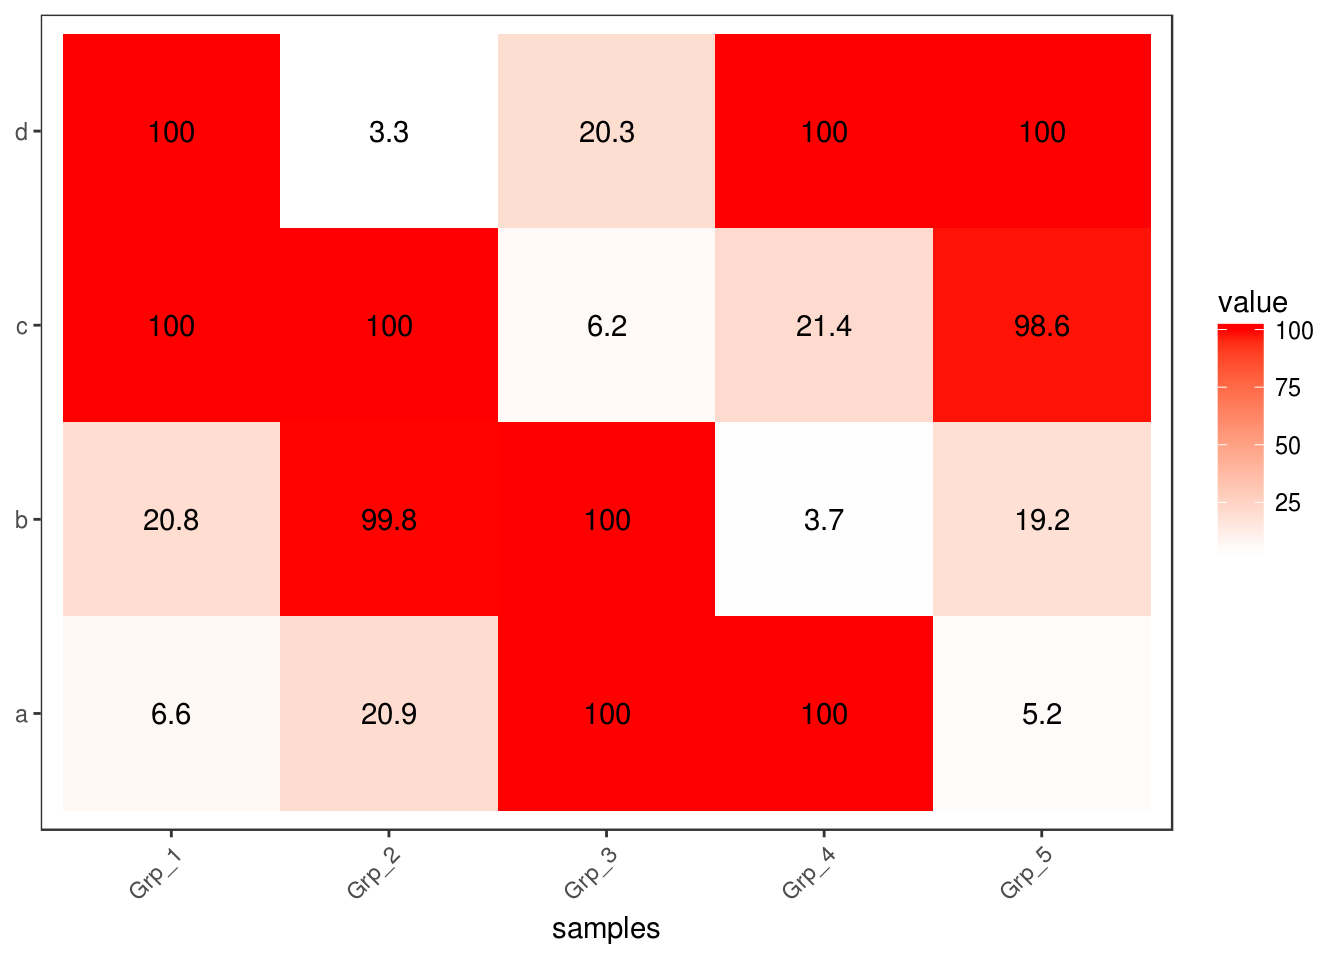
\includegraphics[width=0.95\linewidth,height=0.7\textheight,keepaspectratio]{R_course_files/figure-latex/unnamed-chunk-117-1} \end{center}

虽然损失了一部分信息,但整体模式还是出来了。\textbf{但是在选择异常值标准时需要根据实际确认}。

\subsubsection{非线性颜色}

正常来讲,颜色的赋予在最小值到最大值之间是均匀分布的。如果最小值到最大值之间用100个颜色区分,则其中每一个\texttt{bin},不论其大小、有没有值都会赋予一个颜色。非线性颜色则是对数据比较小但密集的地方赋予更多颜色,数据大但分布散的地方赋予更少颜色,这样既能加大区分度,又最小的影响原始数值。通常可以根据数据模式,手动设置颜色区间。为了方便自动化处理,也可选择用\textbf{四分位数}的方式设置颜色区间。

\begin{Shaded}
\begin{Highlighting}[]
\NormalTok{data_ori <-}\StringTok{ "Grp_1;Grp_2;Grp_3;Grp_4;Grp_5}
\StringTok{a;6.6;20.9;100.1;600.0;5.2}
\StringTok{b;20.8;99.8;700.0;3.7;19.2}
\StringTok{c;100.0;800.0;6.2;21.4;98.6}
\StringTok{d;900;3.3;20.3;101.1;10000"}

\NormalTok{data <-}\StringTok{ }\KeywordTok{read.table}\NormalTok{(}\DataTypeTok{text=}\NormalTok{data_ori, }\DataTypeTok{header=}\NormalTok{T, }\DataTypeTok{row.names=}\DecValTok{1}\NormalTok{, }\DataTypeTok{sep=}\StringTok{";"}\NormalTok{, }\DataTypeTok{quote=}\StringTok{""}\NormalTok{)}

\NormalTok{data}
\end{Highlighting}
\end{Shaded}

\begin{verbatim}
##   Grp_1 Grp_2 Grp_3 Grp_4   Grp_5
## a   6.6  20.9 100.1 600.0     5.2
## b  20.8  99.8 700.0   3.7    19.2
## c 100.0 800.0   6.2  21.4    98.6
## d 900.0   3.3  20.3 101.1 10000.0
\end{verbatim}

获取数据的最大、最小、第一四分位数、中位数、第三四分位数

\begin{Shaded}
\begin{Highlighting}[]
\NormalTok{data$ID =}\StringTok{ }\KeywordTok{rownames}\NormalTok{(data)}
\NormalTok{data_m =}\StringTok{ }\KeywordTok{melt}\NormalTok{(data, }\DataTypeTok{id.vars=}\KeywordTok{c}\NormalTok{(}\StringTok{"ID"}\NormalTok{))}
\NormalTok{summary_v <-}\StringTok{ }\KeywordTok{summary}\NormalTok{(data_m$value)}
\NormalTok{summary_v}
\end{Highlighting}
\end{Shaded}

\begin{verbatim}
##     Min.  1st Qu.   Median     Mean  3rd Qu.     Max. 
##     3.30    16.05    60.00   681.36   225.82 10000.00
\end{verbatim}

在最小值和第一四分位数之间划出6个区间,第一四分位数和中位数之间划出6个区间,中位数和第三四分位数之间划出5个区间,最后的数划出5个区间

\begin{Shaded}
\begin{Highlighting}[]
\NormalTok{break_v <-}\StringTok{ }\KeywordTok{unique}\NormalTok{(}\KeywordTok{c}\NormalTok{(}\KeywordTok{seq}\NormalTok{(summary_v[}\DecValTok{1}\NormalTok{]*}\FloatTok{0.95}\NormalTok{,summary_v[}\DecValTok{2}\NormalTok{],}\DataTypeTok{length=}\DecValTok{6}\NormalTok{), }
        \KeywordTok{seq}\NormalTok{(summary_v[}\DecValTok{2}\NormalTok{],summary_v[}\DecValTok{3}\NormalTok{],}\DataTypeTok{length=}\DecValTok{6}\NormalTok{),}\KeywordTok{seq}\NormalTok{(summary_v[}\DecValTok{3}\NormalTok{],summary_v[}\DecValTok{5}\NormalTok{],}\DataTypeTok{length=}\DecValTok{5}\NormalTok{),}
        \KeywordTok{seq}\NormalTok{(summary_v[}\DecValTok{5}\NormalTok{],summary_v[}\DecValTok{6}\NormalTok{]*}\FloatTok{1.05}\NormalTok{,}\DataTypeTok{length=}\DecValTok{5}\NormalTok{)))}
\NormalTok{break_v}
\end{Highlighting}
\end{Shaded}

\begin{verbatim}
##  [1]     3.1350     5.7180     8.3010    10.8840    13.4670    16.0500
##  [7]    24.8400    33.6300    42.4200    51.2100    60.0000   101.4562
## [13]   142.9125   184.3687   225.8250  2794.3687  5362.9125  7931.4562
## [19] 10500.0000
\end{verbatim}

按照设定的区间分割数据, 原始数据替换为了其所在的区间的数值

\begin{Shaded}
\begin{Highlighting}[]
\NormalTok{data_m$value <-}\StringTok{ }\KeywordTok{cut}\NormalTok{(data_m$value, }\DataTypeTok{breaks=}\NormalTok{break_v,}\DataTypeTok{labels=}\NormalTok{break_v[}\DecValTok{2}\NormalTok{:}\KeywordTok{length}\NormalTok{(break_v)])}
\NormalTok{break_v=}\KeywordTok{unique}\NormalTok{(data_m$value)}

\NormalTok{data_m}
\end{Highlighting}
\end{Shaded}

\begin{verbatim}
##    ID variable      value
## 1   a    Grp_1      8.301
## 2   b    Grp_1      24.84
## 3   c    Grp_1  101.45625
## 4   d    Grp_1 2794.36875
## 5   a    Grp_2      24.84
## 6   b    Grp_2  101.45625
## 7   c    Grp_2 2794.36875
## 8   d    Grp_2      5.718
## 9   a    Grp_3  101.45625
## 10  b    Grp_3 2794.36875
## 11  c    Grp_3      8.301
## 12  d    Grp_3      24.84
## 13  a    Grp_4 2794.36875
## 14  b    Grp_4      5.718
## 15  c    Grp_4      24.84
## 16  d    Grp_4  101.45625
## 17  a    Grp_5      5.718
## 18  b    Grp_5      24.84
## 19  c    Grp_5  101.45625
## 20  d    Grp_5      10500
\end{verbatim}

虽然看上去还是数值,但已经不是数字类型了,而是不同的因子了,这样就可以对不同的因子赋予不同的颜色了

\begin{Shaded}
\begin{Highlighting}[]
\KeywordTok{is.numeric}\NormalTok{(data_m$value)}
\end{Highlighting}
\end{Shaded}

\begin{verbatim}
## [1] FALSE
\end{verbatim}

\begin{Shaded}
\begin{Highlighting}[]
\KeywordTok{is.factor}\NormalTok{(data_m$value)}
\end{Highlighting}
\end{Shaded}

\begin{verbatim}
## [1] TRUE
\end{verbatim}

\begin{Shaded}
\begin{Highlighting}[]
\NormalTok{break_v}
\end{Highlighting}
\end{Shaded}

\begin{verbatim}
## [1] 8.301      24.84      101.45625  2794.36875 5.718      10500     
## 18 Levels: 5.718 8.301 10.884 13.467 16.05 24.84 33.63 42.42 51.21 ... 10500
\end{verbatim}

产生对应数目的颜色

\begin{Shaded}
\begin{Highlighting}[]
\NormalTok{gradientC=}\KeywordTok{c}\NormalTok{(}\StringTok{'green'}\NormalTok{,}\StringTok{'yellow'}\NormalTok{,}\StringTok{'red'}\NormalTok{)}
\NormalTok{col <-}\StringTok{ }\KeywordTok{colorRampPalette}\NormalTok{(gradientC)(}\KeywordTok{length}\NormalTok{(break_v))}
\NormalTok{col}
\end{Highlighting}
\end{Shaded}

\begin{verbatim}
## [1] "#00FF00" "#66FF00" "#CCFF00" "#FFCB00" "#FF6500" "#FF0000"
\end{verbatim}

\begin{Shaded}
\begin{Highlighting}[]
\NormalTok{p <-}\StringTok{ }\KeywordTok{ggplot}\NormalTok{(data_m, }\KeywordTok{aes}\NormalTok{(}\DataTypeTok{x=}\NormalTok{variable,}\DataTypeTok{y=}\NormalTok{ID)) +}\StringTok{ }\KeywordTok{xlab}\NormalTok{(}\StringTok{"samples"}\NormalTok{) +}\StringTok{ }\KeywordTok{ylab}\NormalTok{(}\OtherTok{NULL}\NormalTok{) +}\StringTok{ }\KeywordTok{theme_bw}\NormalTok{() +}\StringTok{ }
\StringTok{    }\KeywordTok{theme}\NormalTok{(}\DataTypeTok{panel.grid.major =} \KeywordTok{element_blank}\NormalTok{()) +}\StringTok{ }\KeywordTok{theme}\NormalTok{(}\DataTypeTok{legend.key=}\KeywordTok{element_blank}\NormalTok{()) +}\StringTok{ }
\StringTok{    }\KeywordTok{theme}\NormalTok{(}\DataTypeTok{axis.text.x=}\KeywordTok{element_text}\NormalTok{(}\DataTypeTok{angle=}\DecValTok{45}\NormalTok{,}\DataTypeTok{hjust=}\DecValTok{1}\NormalTok{, }\DataTypeTok{vjust=}\DecValTok{1}\NormalTok{)) +}\StringTok{ }\KeywordTok{geom_tile}\NormalTok{(}\KeywordTok{aes}\NormalTok{(}\DataTypeTok{fill=}\NormalTok{value))}

\CommentTok{# 与上面不同的地方,使用的是scale_fill_manual逐个赋值}
\NormalTok{p <-}\StringTok{ }\NormalTok{p +}\StringTok{ }\KeywordTok{scale_fill_manual}\NormalTok{(}\DataTypeTok{values=}\NormalTok{col)}
\NormalTok{p}
\CommentTok{#ggsave(p, filename="heatmap_nonlinear.pdf", width=8, height=12, units=c("cm"),colormodel="srgb")}
\end{Highlighting}
\end{Shaded}

\begin{center}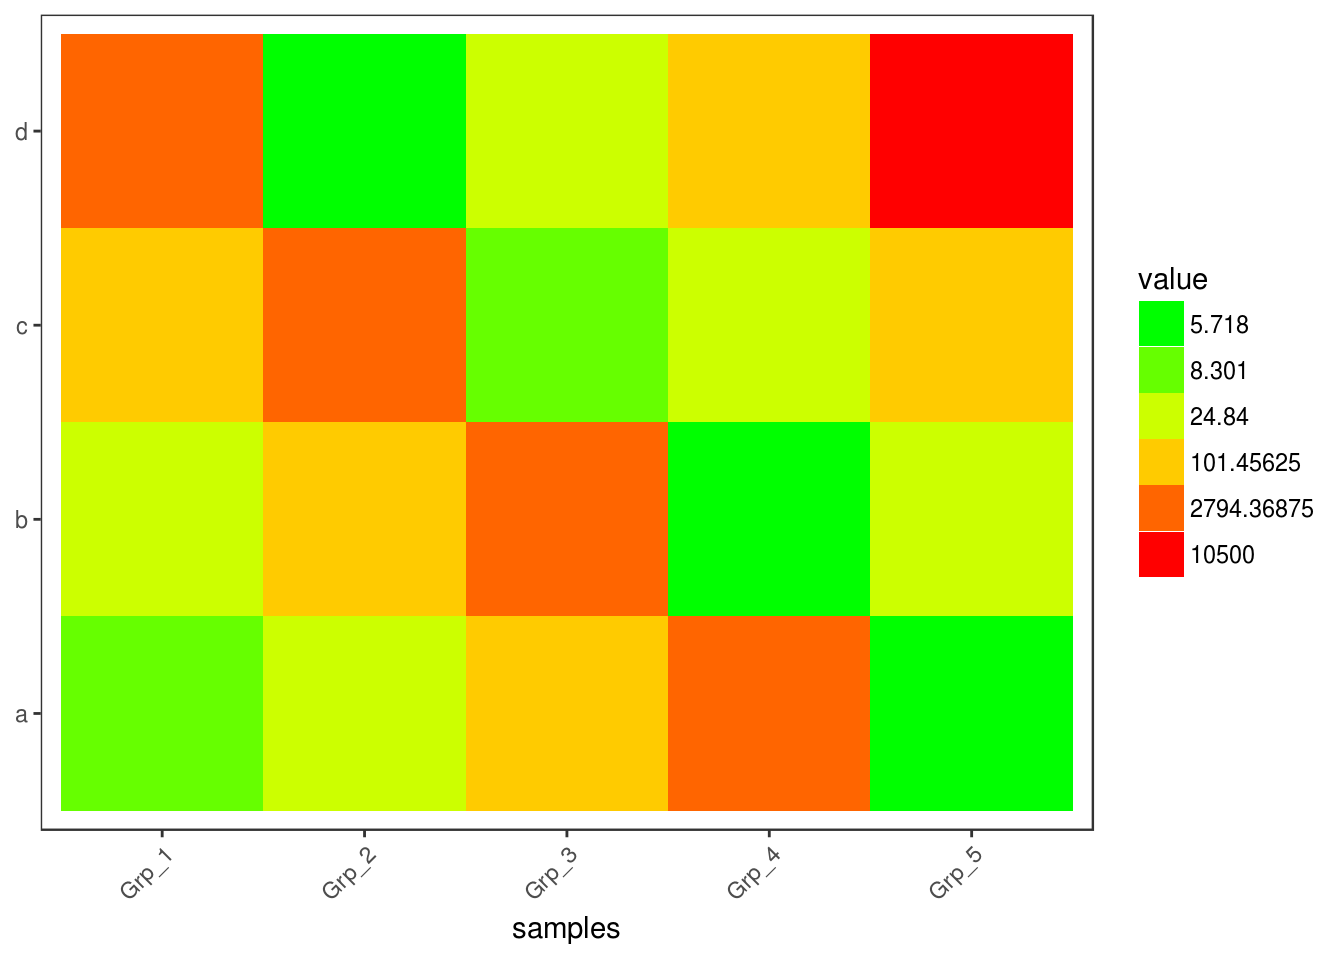
\includegraphics[width=0.95\linewidth,height=0.7\textheight,keepaspectratio]{R_course_files/figure-latex/unnamed-chunk-126-1} \end{center}

\subsubsection{调整行或列的顺序}

如果想保持图中每一行的顺序与输入的数据框一致,需要设置因子的水平。这也是\texttt{ggplot2}中调整图例或横纵轴字符顺序的常用方式。

\begin{Shaded}
\begin{Highlighting}[]
\NormalTok{data_rowname <-}\StringTok{ }\KeywordTok{rownames}\NormalTok{(data)}
\NormalTok{data_rowname <-}\StringTok{ }\KeywordTok{as.vector}\NormalTok{(}\KeywordTok{rownames}\NormalTok{(data))}
\NormalTok{data_rownames <-}\StringTok{ }\KeywordTok{rev}\NormalTok{(data_rowname)}
\NormalTok{data_log_m$ID <-}\StringTok{ }\KeywordTok{factor}\NormalTok{(data_log_m$ID, }\DataTypeTok{levels=}\NormalTok{data_rownames, }\DataTypeTok{ordered=}\NormalTok{T)}
\NormalTok{p <-}\StringTok{ }\KeywordTok{ggplot}\NormalTok{(data_log_m, }\KeywordTok{aes}\NormalTok{(}\DataTypeTok{x=}\NormalTok{variable,}\DataTypeTok{y=}\NormalTok{ID)) +}\StringTok{ }\KeywordTok{xlab}\NormalTok{(}\OtherTok{NULL}\NormalTok{) +}\StringTok{ }\KeywordTok{ylab}\NormalTok{(}\OtherTok{NULL}\NormalTok{) +}\StringTok{ }\KeywordTok{theme_bw}\NormalTok{() +}\StringTok{ }
\StringTok{    }\KeywordTok{theme}\NormalTok{(}\DataTypeTok{panel.grid.major =} \KeywordTok{element_blank}\NormalTok{()) +}\StringTok{ }\KeywordTok{theme}\NormalTok{(}\DataTypeTok{legend.key=}\KeywordTok{element_blank}\NormalTok{()) +}\StringTok{ }
\StringTok{    }\KeywordTok{theme}\NormalTok{(}\DataTypeTok{axis.text.x=}\KeywordTok{element_text}\NormalTok{(}\DataTypeTok{angle=}\DecValTok{45}\NormalTok{,}\DataTypeTok{hjust=}\DecValTok{1}\NormalTok{, }\DataTypeTok{vjust=}\DecValTok{1}\NormalTok{)) +}\StringTok{ }
\StringTok{    }\KeywordTok{theme}\NormalTok{(}\DataTypeTok{legend.position=}\StringTok{"top"}\NormalTok{) +}\StringTok{  }\KeywordTok{geom_tile}\NormalTok{(}\KeywordTok{aes}\NormalTok{(}\DataTypeTok{fill=}\NormalTok{value)) +}\StringTok{ }
\StringTok{    }\KeywordTok{scale_fill_gradient}\NormalTok{(}\DataTypeTok{low =} \StringTok{"white"}\NormalTok{, }\DataTypeTok{high =} \StringTok{"red"}\NormalTok{)}
\NormalTok{p}
\CommentTok{#ggsave(p, filename="heatmap_log.pdf", width=8, height=12, units=c("cm"),colormodel="srgb")}
\end{Highlighting}
\end{Shaded}

\begin{center}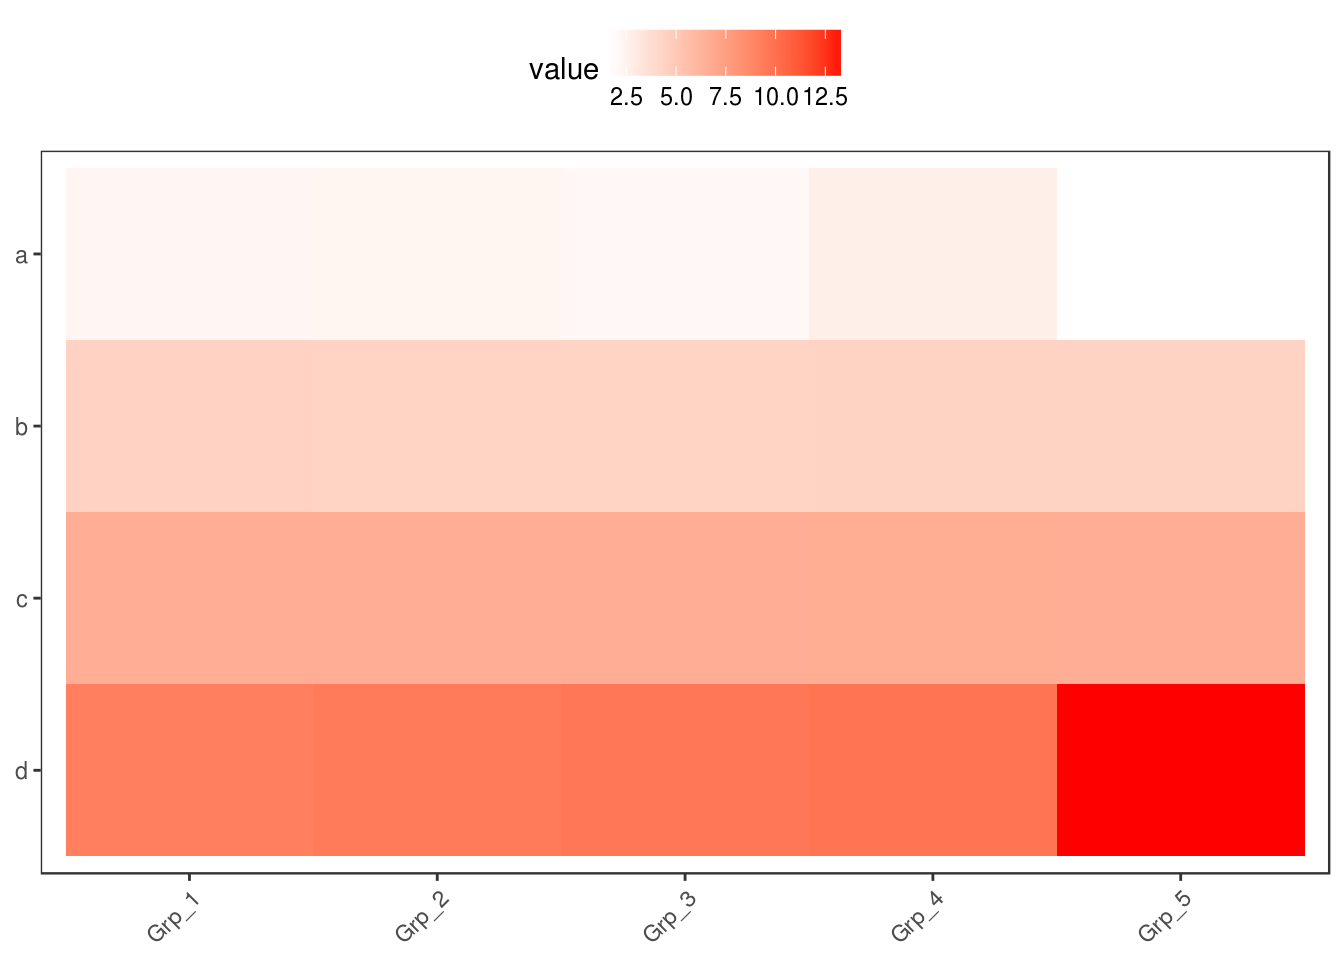
\includegraphics[width=0.95\linewidth,height=0.7\textheight,keepaspectratio]{R_course_files/figure-latex/unnamed-chunk-127-1} \end{center}

基于ggplot2的heatmap绘制到现在就差不多了,但总是这么画下去也会觉得有点累,有没有办法更简化呢?。

\subsection{热图绘制 - pheatmap}\label{---pheatmap}

绘制热图除了使用\texttt{ggplot2},还可以有其它的包或函数,比如\texttt{pheatmap::pheatmap}
(pheatmap包中的pheatmap函数)、\texttt{gplots::heatmap.2}等。

相比于\texttt{ggplot2}作heatmap,
\texttt{pheatmap}会更为简单一些,一个函数设置不同的参数,可以完成行列聚类、行列注释、\texttt{Z-score}计算、颜色自定义等。那我们来看看效果怎样。

\begin{Shaded}
\begin{Highlighting}[]
\NormalTok{data_ori <-}\StringTok{ "Grp_1;Grp_2;Grp_3;Grp_4;Grp_5}
\StringTok{a;6.6;20.9;100.1;600.0;5.2}
\StringTok{b;20.8;99.8;700.0;3.7;19.2}
\StringTok{c;100.0;800.0;6.2;21.4;98.6}
\StringTok{d;900;3.3;20.3;101.1;10000"}

\NormalTok{data <-}\StringTok{ }\KeywordTok{read.table}\NormalTok{(}\DataTypeTok{text=}\NormalTok{data_ori, }\DataTypeTok{header=}\NormalTok{T, }\DataTypeTok{row.names=}\DecValTok{1}\NormalTok{, }\DataTypeTok{sep=}\StringTok{";"}\NormalTok{, }\DataTypeTok{quote=}\StringTok{""}\NormalTok{)}
\end{Highlighting}
\end{Shaded}

\begin{Shaded}
\begin{Highlighting}[]
\CommentTok{#pheatmap::pheatmap(data, filename="pheatmap_1.pdf")}
\NormalTok{pheatmap::}\KeywordTok{pheatmap}\NormalTok{(data)}
\end{Highlighting}
\end{Shaded}

\begin{center}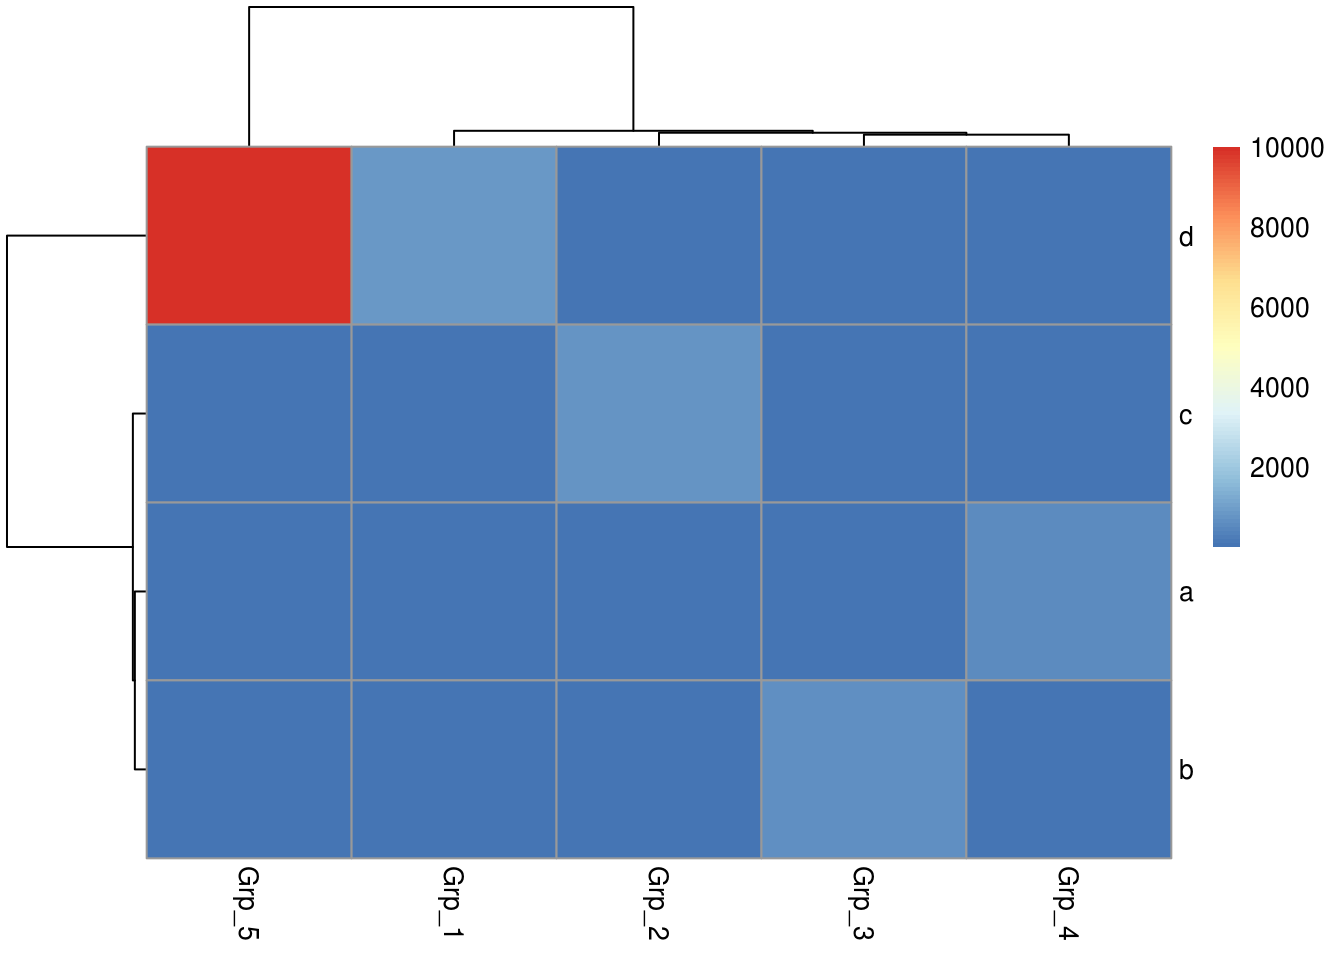
\includegraphics[width=0.95\linewidth,height=0.7\textheight,keepaspectratio]{R_course_files/figure-latex/unnamed-chunk-129-1} \end{center}

虽然有点丑,但一步就出来了。

在\texttt{heatmap美化}篇提到的数据前期处理方式,都可以用于\texttt{pheatmap}的画图。此外\texttt{Z-score}计算在\texttt{pheatmap}中只要一个参数就可以实现。

\begin{Shaded}
\begin{Highlighting}[]
\NormalTok{pheatmap::}\KeywordTok{pheatmap}\NormalTok{(data, }\DataTypeTok{scale=}\StringTok{"row"}\NormalTok{)}
\end{Highlighting}
\end{Shaded}

\begin{center}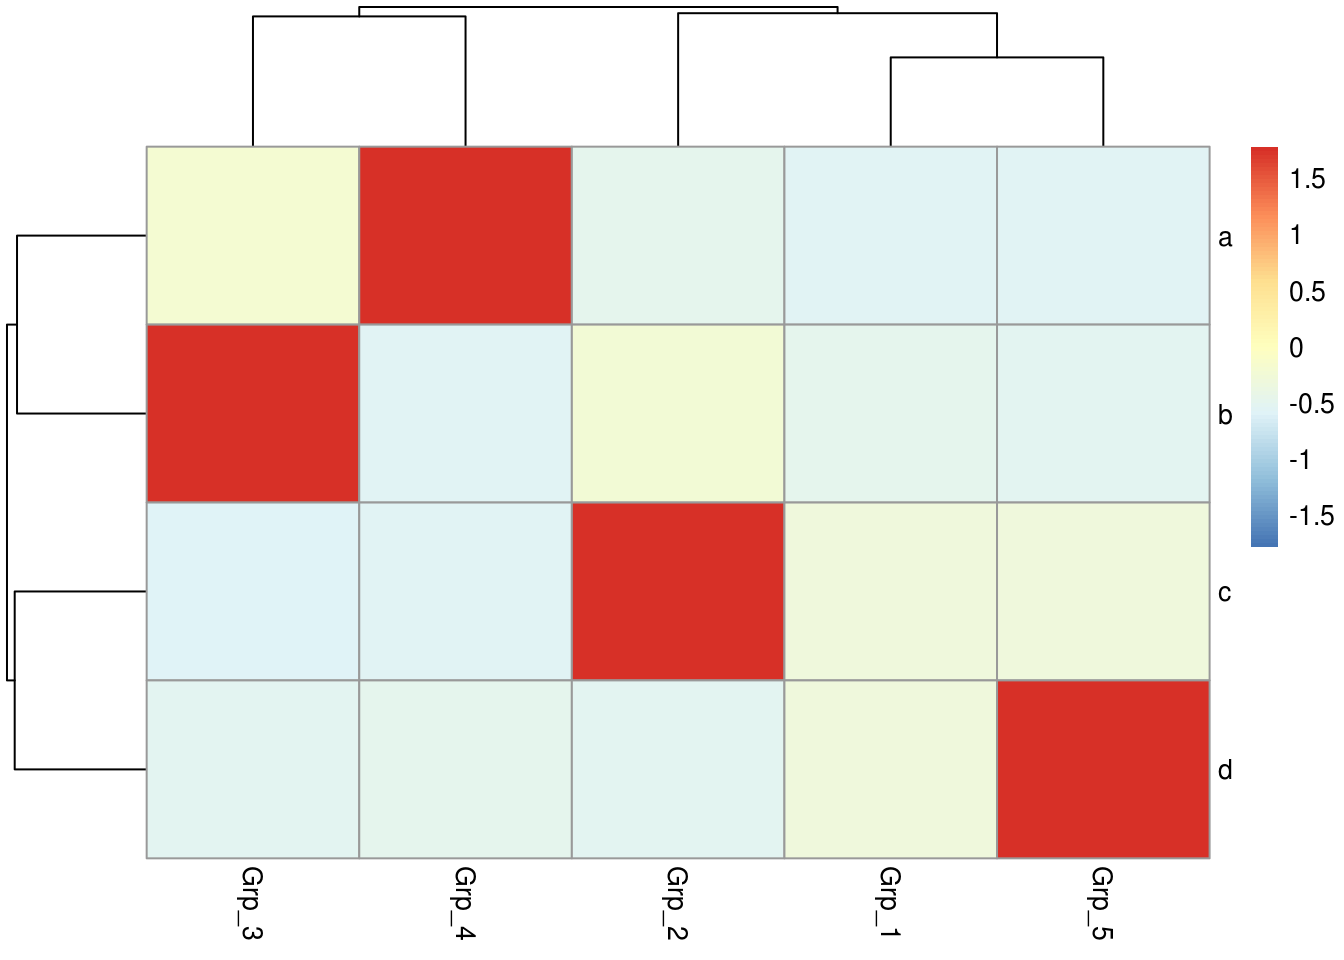
\includegraphics[width=0.95\linewidth,height=0.7\textheight,keepaspectratio]{R_course_files/figure-latex/unnamed-chunk-130-1} \end{center}

有时可能不需要行或列的聚类,原始展示就可以了。

\begin{Shaded}
\begin{Highlighting}[]
\NormalTok{pheatmap::}\KeywordTok{pheatmap}\NormalTok{(data, }\DataTypeTok{scale=}\StringTok{"row"}\NormalTok{, }\DataTypeTok{cluster_rows=}\OtherTok{FALSE}\NormalTok{, }\DataTypeTok{cluster_cols=}\OtherTok{FALSE}\NormalTok{)}
\end{Highlighting}
\end{Shaded}

\begin{center}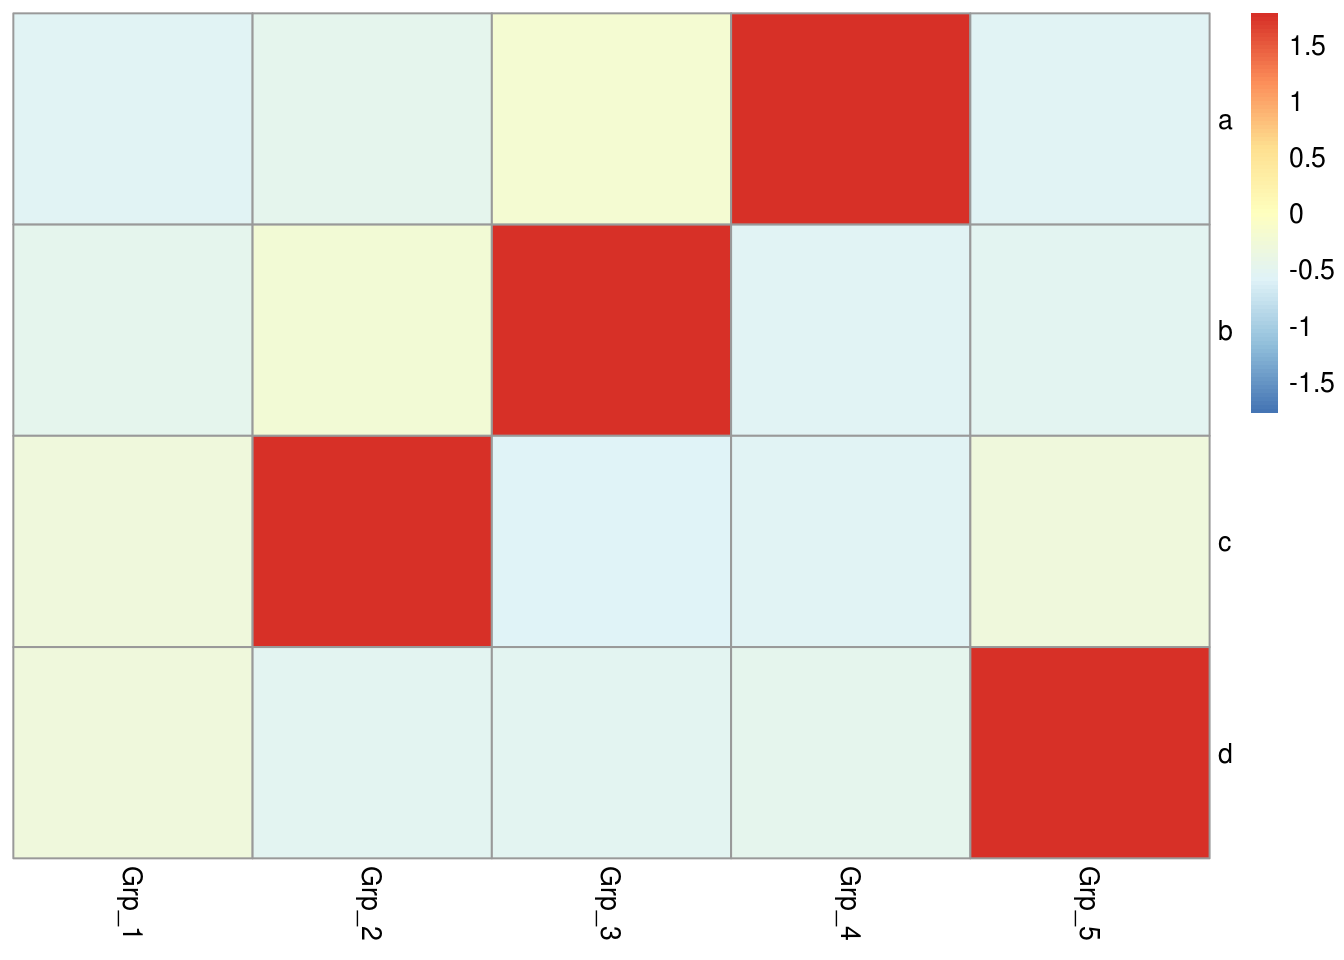
\includegraphics[width=0.95\linewidth,height=0.7\textheight,keepaspectratio]{R_course_files/figure-latex/unnamed-chunk-131-1} \end{center}

给矩阵
(\texttt{data})中行和列不同的分组注释。假如有两个文件,第一个文件为行注释,其第一列与矩阵中的第一列内容相同
(顺序没有关系),其它列为第一列的不同的标记,如下面示例中(假设行为基因,列为样品)的2,3列对应基因的不同类型
(TF or
enzyme)和不同分组。第二个文件为列注释,其第一列与矩阵中第一行内容相同,其它列则为样品的注释。

\begin{Shaded}
\begin{Highlighting}[]
\NormalTok{row_anno =}\StringTok{ }\KeywordTok{data.frame}\NormalTok{(}\DataTypeTok{type=}\KeywordTok{c}\NormalTok{(}\StringTok{"TF"}\NormalTok{,}\StringTok{"Enzyme"}\NormalTok{,}\StringTok{"Enzyme"}\NormalTok{,}\StringTok{"TF"}\NormalTok{), }
        \DataTypeTok{class=}\KeywordTok{c}\NormalTok{(}\StringTok{"clu1"}\NormalTok{,}\StringTok{"clu1"}\NormalTok{,}\StringTok{"clu2"}\NormalTok{,}\StringTok{"clu2"}\NormalTok{), }\DataTypeTok{row.names=}\KeywordTok{rownames}\NormalTok{(data))}
\NormalTok{row_anno}
\end{Highlighting}
\end{Shaded}

\begin{verbatim}
##     type class
## a     TF  clu1
## b Enzyme  clu1
## c Enzyme  clu2
## d     TF  clu2
\end{verbatim}

\begin{Shaded}
\begin{Highlighting}[]
\NormalTok{col_anno =}\StringTok{ }\KeywordTok{data.frame}\NormalTok{(}\DataTypeTok{grp=}\KeywordTok{c}\NormalTok{(}\StringTok{"A"}\NormalTok{,}\StringTok{"A"}\NormalTok{,}\StringTok{"A"}\NormalTok{,}\StringTok{"B"}\NormalTok{,}\StringTok{"B"}\NormalTok{), }\DataTypeTok{size=}\DecValTok{1}\NormalTok{:}\DecValTok{5}\NormalTok{, }\DataTypeTok{row.names=}\KeywordTok{colnames}\NormalTok{(data))}
\NormalTok{col_anno}
\end{Highlighting}
\end{Shaded}

\begin{verbatim}
##       grp size
## Grp_1   A    1
## Grp_2   A    2
## Grp_3   A    3
## Grp_4   B    4
## Grp_5   B    5
\end{verbatim}

\begin{Shaded}
\begin{Highlighting}[]
\NormalTok{pheatmap::}\KeywordTok{pheatmap}\NormalTok{(data, }\DataTypeTok{scale=}\StringTok{"row"}\NormalTok{, }
\DataTypeTok{cluster_rows=}\OtherTok{FALSE}\NormalTok{, }\DataTypeTok{annotation_col=}\NormalTok{col_anno, }\DataTypeTok{annotation_row=}\NormalTok{row_anno)}
\end{Highlighting}
\end{Shaded}

\begin{center}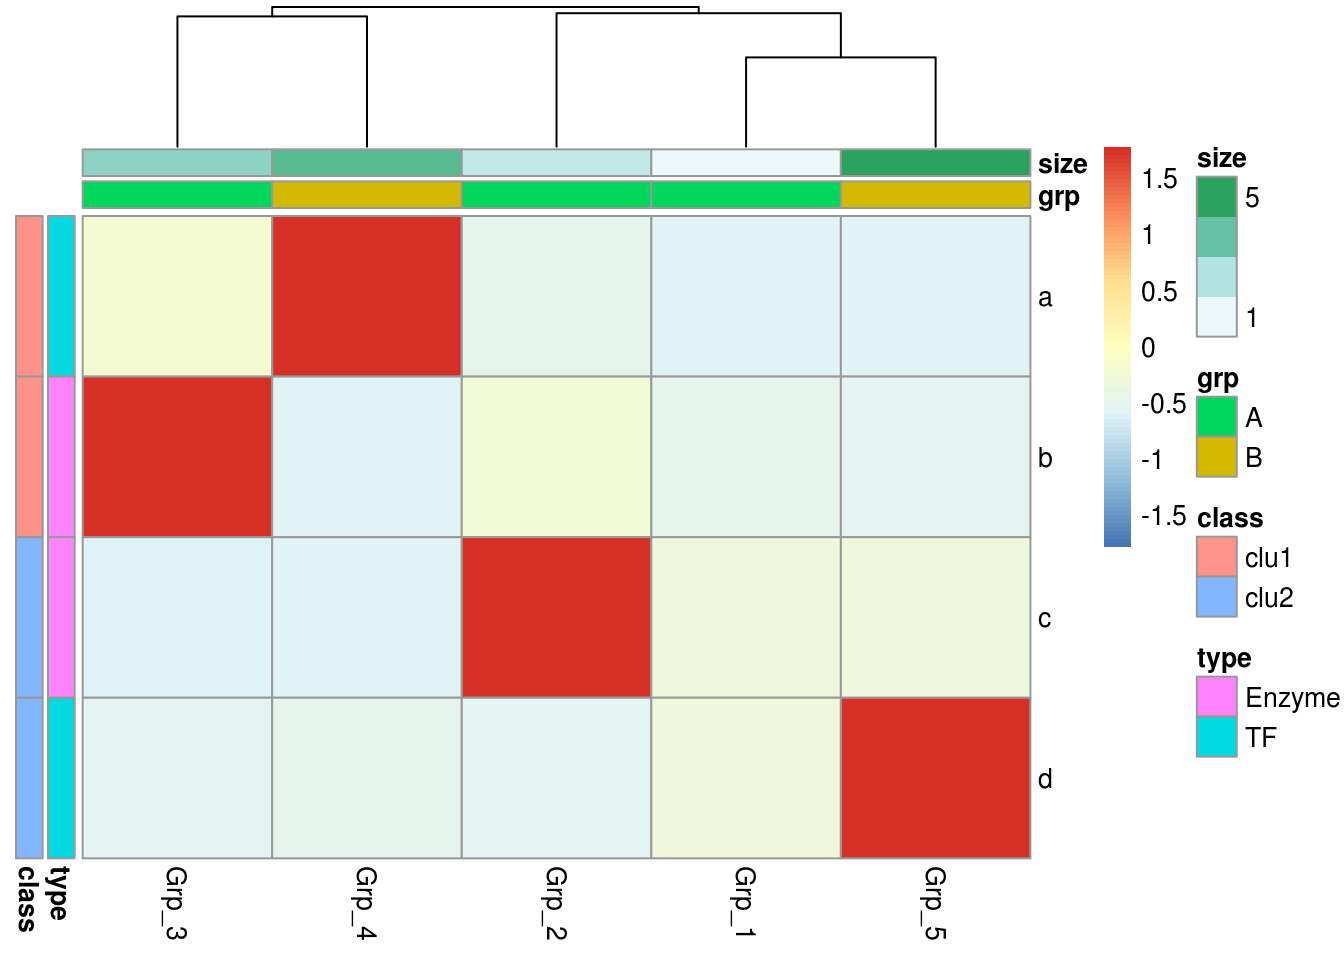
\includegraphics[width=0.95\linewidth,height=0.7\textheight,keepaspectratio]{R_course_files/figure-latex/unnamed-chunk-134-1} \end{center}

自定义下颜色吧。

\begin{Shaded}
\begin{Highlighting}[]
\CommentTok{# <bias> values larger than 1 will give more color for high end. }
\CommentTok{# Values between 0-1 will give more color for low end.}
\NormalTok{pheatmap::}\KeywordTok{pheatmap}\NormalTok{(data, }\DataTypeTok{scale=}\StringTok{"row"}\NormalTok{, }\DataTypeTok{cluster_rows=}\OtherTok{FALSE}\NormalTok{, }
\DataTypeTok{annotation_col=}\NormalTok{col_anno, }\DataTypeTok{annotation_row=}\NormalTok{row_anno,}
\DataTypeTok{color=}\KeywordTok{colorRampPalette}\NormalTok{(}\KeywordTok{c}\NormalTok{(}\StringTok{'green'}\NormalTok{,}\StringTok{'yellow'}\NormalTok{,}\StringTok{'red'}\NormalTok{), }\DataTypeTok{bias=}\DecValTok{1}\NormalTok{)(}\DecValTok{50}\NormalTok{))}
\end{Highlighting}
\end{Shaded}

\begin{center}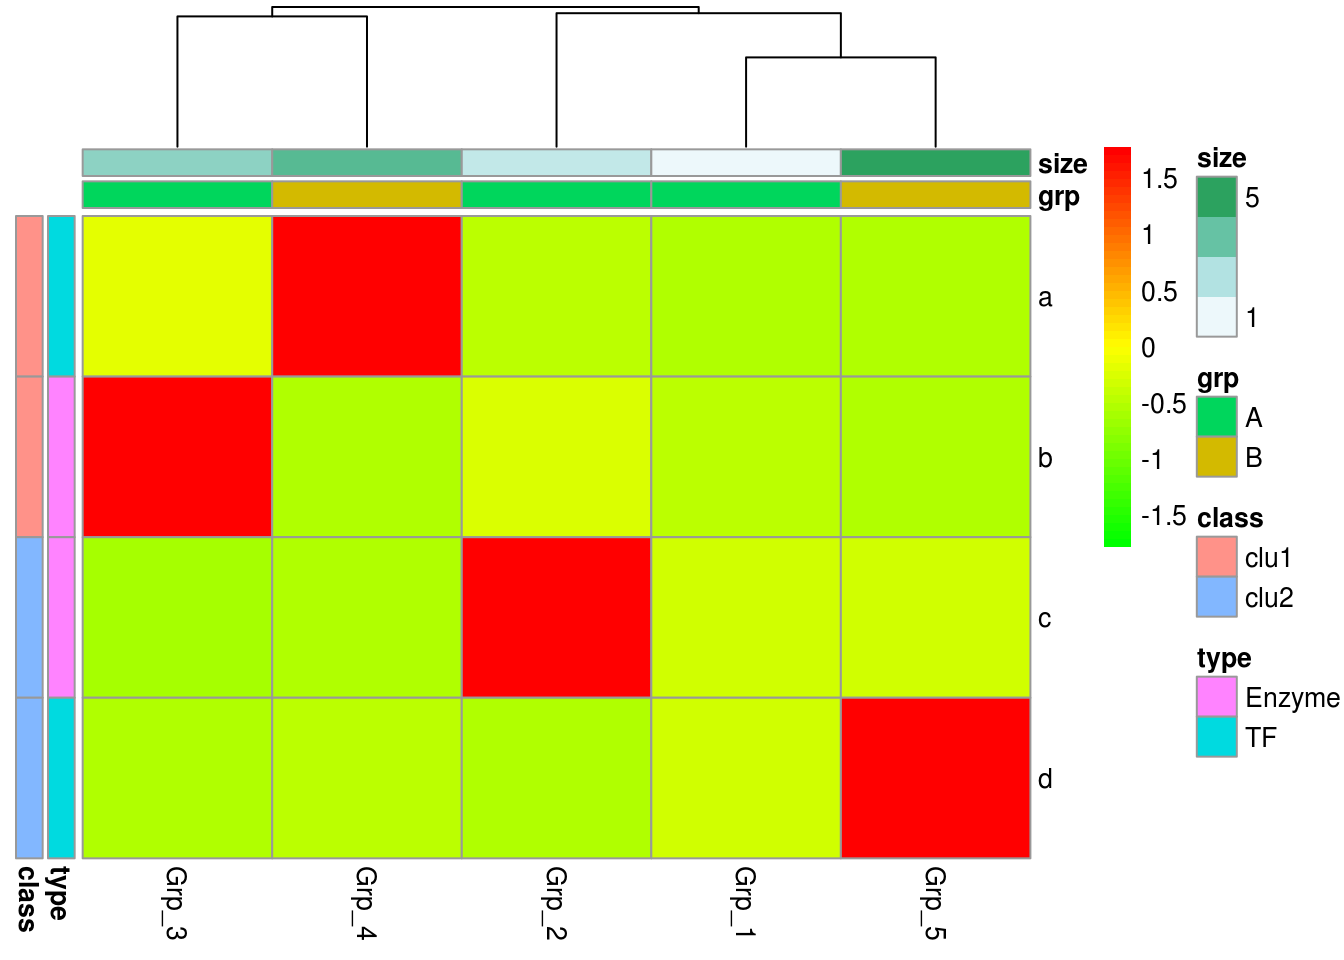
\includegraphics[width=0.95\linewidth,height=0.7\textheight,keepaspectratio]{R_course_files/figure-latex/unnamed-chunk-135-1} \end{center}

\texttt{heatmap.2}的使用在上一期转录组分析绘制相关性热图时有提到,这次就不介绍了,跟\texttt{pheatmap}有些类似,而且也有不少教程。

\subsection{箱线图}

箱线图是能同时反映数据统计量和整体分布,又很漂亮的展示图。在2014年的Nature
Method上有2篇\texttt{Correspondence}论述了使用箱线图的好处和一个在线绘制箱线图的工具。就这样都可以发两篇Nature
method,没天理,但也说明了箱线图的重要意义。

下面这张图展示了\texttt{Bar\ plot}、\texttt{Box\ plot}、\texttt{Volin\ plot}和\texttt{Bean\ plot}对数据分布的反应。从Bar
plot上只能看到数据标准差或标准误不同;Box
plot可以看到数据分布的集中性不同;Violin plot和Bean
plot展示的是数据真正的分布,尤其是对Biomodal数据的展示。

Boxplot从下到上展示的是最小值,第一四分位数 (箱子的下边线)、中位数
(箱子中间的线)、第三四分位数 (箱子上边线)、最大值,具体解读参见
\url{http://mp.weixin.qq.com/s/t3UTI_qAIi0cy1g6ZmHtwg}。

\begin{center}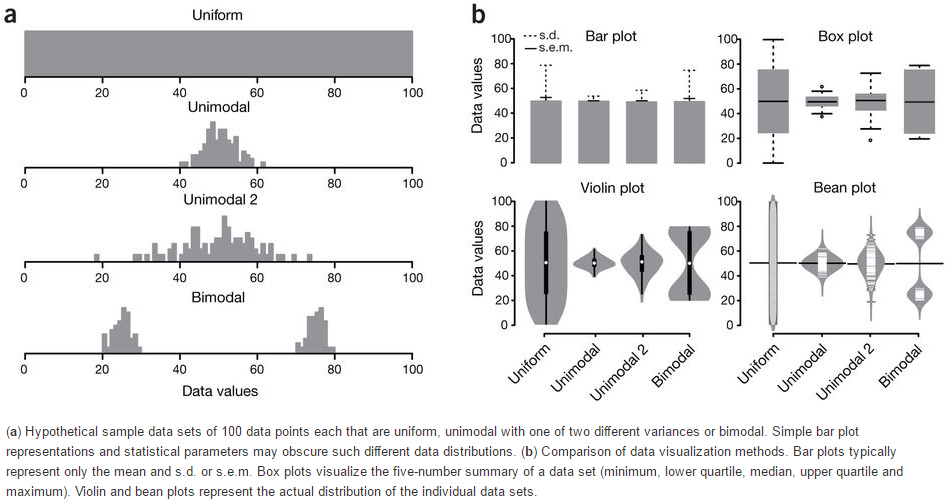
\includegraphics[width=0.95\linewidth,height=0.7\textheight,keepaspectratio]{images/boxplot_nm} \end{center}

\begin{itemize}
\tightlist
\item
  Nature Method文章
  \url{http://www.nature.com/nmeth/journal/v11/n2/full/nmeth.2811.html}
\end{itemize}

\subsubsection{一步步解析箱线图绘制}

假设有这么一个基因表达矩阵,第一列为基因名字,第一行为样品名字,想绘制样品中基因表达的整体分布。

\begin{Shaded}
\begin{Highlighting}[]
\NormalTok{profile=}\StringTok{"Name;2cell_1;2cell_2;2cell_3;4cell_1;4cell_2;4cell_3;zygote_1;zygote_2;zygote_3}
\StringTok{A;4;6;7;3.2;5.2;5.6;2;4;3}
\StringTok{B;6;8;9;5.2;7.2;7.6;4;6;5}
\StringTok{C;8;10;11;7.2;9.2;9.6;6;8;7}
\StringTok{D;10;12;13;9.2;11.2;11.6;8;10;9}
\StringTok{E;12;14;15;11.2;13.2;13.6;10;12;11}
\StringTok{F;14;16;17;13.2;15.2;15.6;12;14;13}
\StringTok{G;15;17;18;14.2;16.2;16.6;13;15;14}
\StringTok{H;16;18;19;15.2;17.2;17.6;14;16;15}
\StringTok{I;17;19;20;16.2;18.2;18.6;15;17;16}
\StringTok{J;18;20;21;17.2;19.2;19.6;16;18;17}
\StringTok{L;19;21;22;18.2;20.2;20.6;17;19;18}
\StringTok{M;20;22;23;19.2;21.2;21.6;18;20;19}
\StringTok{N;21;23;24;20.2;22.2;22.6;19;21;20}
\StringTok{O;22;24;25;21.2;23.2;23.6;20;22;21"}
\end{Highlighting}
\end{Shaded}

读入数据并转换为ggplot2需要的长数据表格式,好好体会下这个格式,虽然多占用了不少空间,但是确实很方便。

\begin{Shaded}
\begin{Highlighting}[]
\NormalTok{profile_text <-}\StringTok{ }\KeywordTok{read.table}\NormalTok{(}\DataTypeTok{text=}\NormalTok{profile, }\DataTypeTok{header=}\NormalTok{T, }\DataTypeTok{row.names=}\DecValTok{1}\NormalTok{, }\DataTypeTok{quote=}\StringTok{""}\NormalTok{,}\DataTypeTok{sep=}\StringTok{";"}\NormalTok{, }\DataTypeTok{check.names=}\NormalTok{F)}
\CommentTok{# 在melt时保留位置信息}
\CommentTok{# melt格式是ggplot2画图最喜欢的格式}
\CommentTok{# }

\KeywordTok{library}\NormalTok{(ggplot2)}
\KeywordTok{library}\NormalTok{(reshape2)}
\NormalTok{data_m <-}\StringTok{ }\KeywordTok{melt}\NormalTok{(profile_text)}
\end{Highlighting}
\end{Shaded}

\begin{verbatim}
## No id variables; using all as measure variables
\end{verbatim}

\begin{Shaded}
\begin{Highlighting}[]
\KeywordTok{head}\NormalTok{(data_m)}
\end{Highlighting}
\end{Shaded}

\begin{verbatim}
##   variable value
## 1  2cell_1     4
## 2  2cell_1     6
## 3  2cell_1     8
## 4  2cell_1    10
## 5  2cell_1    12
## 6  2cell_1    14
\end{verbatim}

\begin{Shaded}
\begin{Highlighting}[]
\KeywordTok{summary}\NormalTok{(data_m)}
\end{Highlighting}
\end{Shaded}

\begin{verbatim}
##     variable      value      
##  2cell_1:14   Min.   : 2.00  
##  2cell_2:14   1st Qu.:10.25  
##  2cell_3:14   Median :16.00  
##  4cell_1:14   Mean   :14.87  
##  4cell_2:14   3rd Qu.:19.20  
##  4cell_3:14   Max.   :25.00  
##  (Other):42
\end{verbatim}

\texttt{variable}和\texttt{value}为矩阵\texttt{melt}后的两列的名字,内部变量,
可以通过\texttt{?melt}查看如何修改。\texttt{variable}代表了点线的属性,\texttt{value}代表对应的值。
像往常一样,就可以直接画图了。

\begin{Shaded}
\begin{Highlighting}[]
\NormalTok{p <-}\StringTok{ }\KeywordTok{ggplot}\NormalTok{(data_m, }\KeywordTok{aes}\NormalTok{(}\DataTypeTok{x=}\NormalTok{variable, }\DataTypeTok{y=}\NormalTok{value,}\DataTypeTok{color=}\NormalTok{variable)) +}\StringTok{ }
\KeywordTok{geom_boxplot}\NormalTok{() +}\StringTok{ }
\KeywordTok{theme}\NormalTok{(}\DataTypeTok{axis.text.x=}\KeywordTok{element_text}\NormalTok{(}\DataTypeTok{angle=}\DecValTok{50}\NormalTok{,}\DataTypeTok{hjust=}\FloatTok{0.5}\NormalTok{, }\DataTypeTok{vjust=}\FloatTok{0.5}\NormalTok{)) +}
\KeywordTok{theme}\NormalTok{(}\DataTypeTok{legend.position=}\StringTok{"none"}\NormalTok{)}
\NormalTok{p}
\CommentTok{# 图会存储在当前目录的Rplots.pdf文件中,如果用Rstudio,可以不运行dev.off()}
\CommentTok{# dev.off()}
\end{Highlighting}
\end{Shaded}

\begin{center}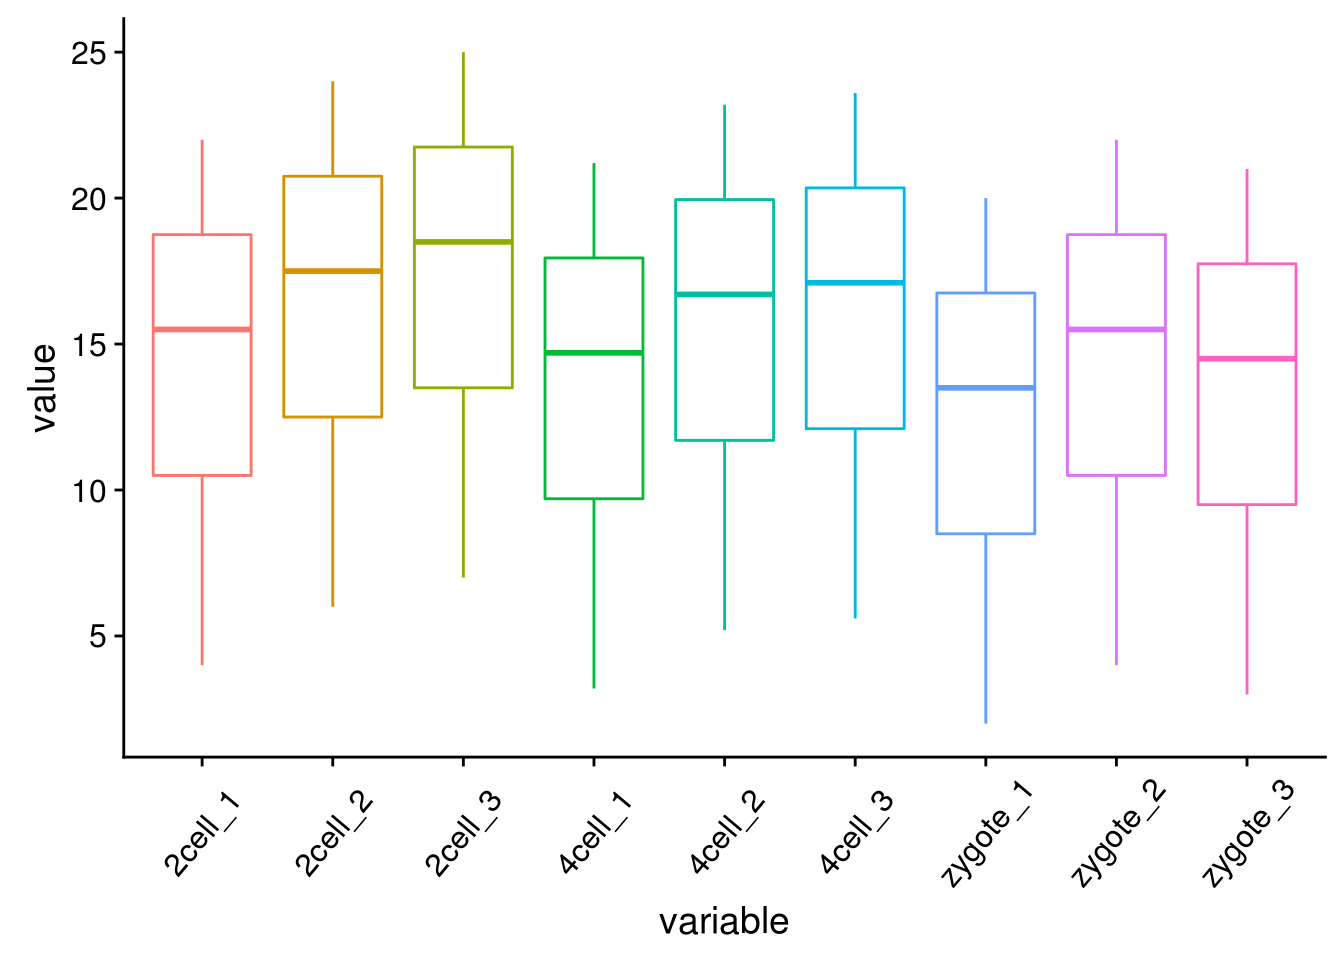
\includegraphics[width=0.95\linewidth,height=0.7\textheight,keepaspectratio]{R_course_files/figure-latex/unnamed-chunk-140-1} \end{center}

箱线图出来了,看上去还可以,再加点色彩 (\texttt{fill})。

\begin{Shaded}
\begin{Highlighting}[]
\CommentTok{# variable和value为矩阵melt后的两列的名字,内部变量, variable代表了点线的属性,value代表对应的值。}
\NormalTok{p <-}\StringTok{ }\KeywordTok{ggplot}\NormalTok{(data_m, }\KeywordTok{aes}\NormalTok{(}\DataTypeTok{x=}\NormalTok{variable, }\DataTypeTok{y=}\NormalTok{value)) +}\StringTok{ }
\KeywordTok{geom_boxplot}\NormalTok{(}\KeywordTok{aes}\NormalTok{(}\DataTypeTok{fill=}\KeywordTok{factor}\NormalTok{(variable))) +}\StringTok{ }
\KeywordTok{theme}\NormalTok{(}\DataTypeTok{axis.text.x=}\KeywordTok{element_text}\NormalTok{(}\DataTypeTok{angle=}\DecValTok{50}\NormalTok{,}\DataTypeTok{hjust=}\FloatTok{0.5}\NormalTok{, }\DataTypeTok{vjust=}\FloatTok{0.5}\NormalTok{)) +}
\KeywordTok{theme}\NormalTok{(}\DataTypeTok{legend.position=}\StringTok{"none"}\NormalTok{)}
\NormalTok{p}
\CommentTok{# 图会存储在当前目录的Rplots.pdf文件中,如果用Rstudio,可以不运行dev.off()}
\CommentTok{#dev.off()}
\end{Highlighting}
\end{Shaded}

\begin{center}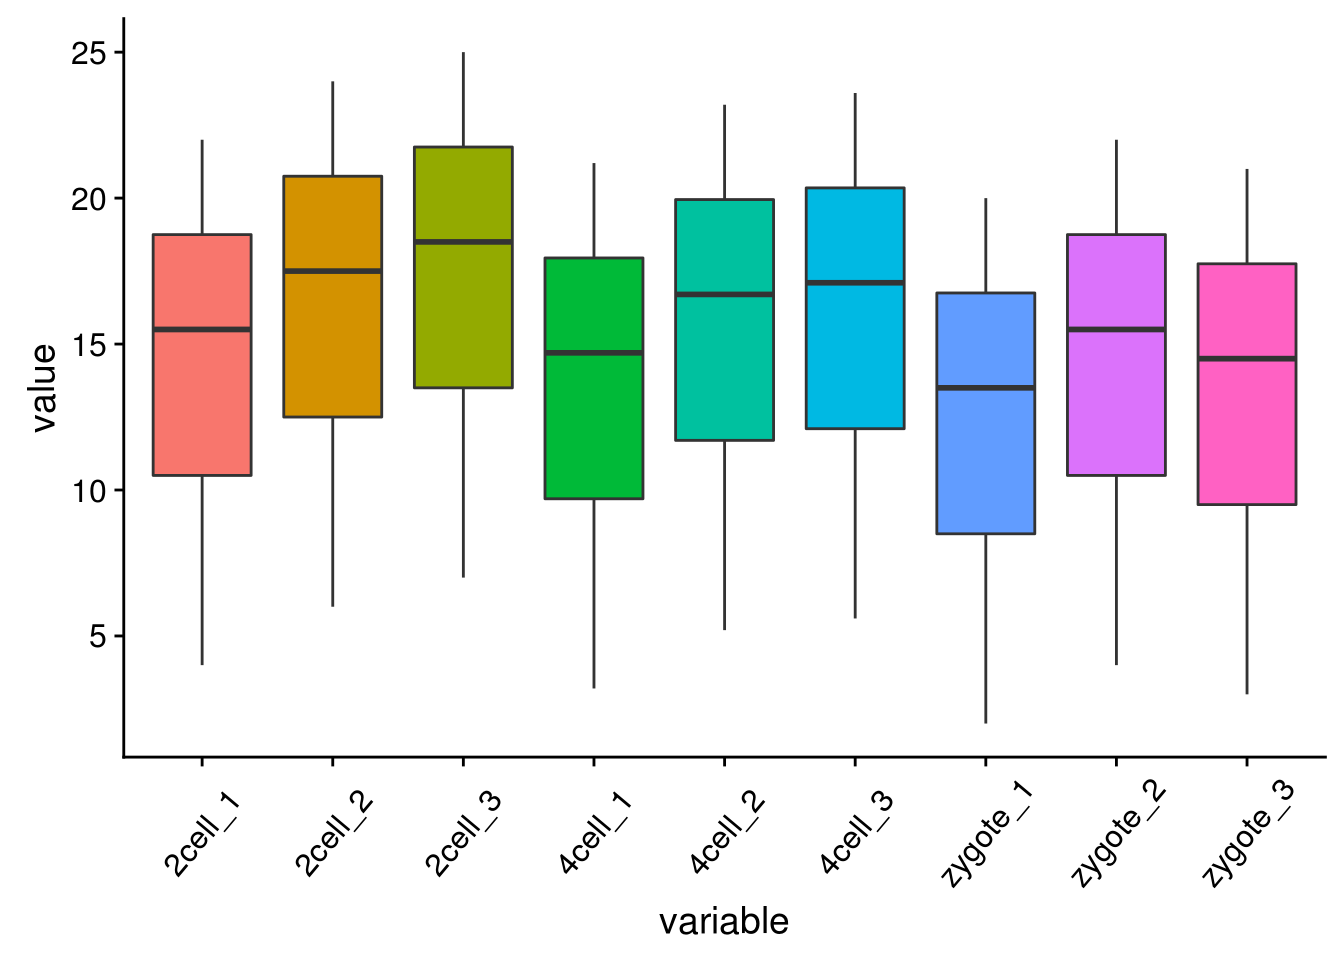
\includegraphics[width=0.95\linewidth,height=0.7\textheight,keepaspectratio]{R_course_files/figure-latex/unnamed-chunk-141-1} \end{center}

再看看\texttt{Violin\ plot}

\begin{Shaded}
\begin{Highlighting}[]
\CommentTok{# variable和value为矩阵melt后的两列的名字,内部变量, variable代表了点线的属性,value代表对应的值。}
\NormalTok{p <-}\StringTok{ }\KeywordTok{ggplot}\NormalTok{(data_m, }\KeywordTok{aes}\NormalTok{(}\DataTypeTok{x=}\NormalTok{variable, }\DataTypeTok{y=}\NormalTok{value)) +}\StringTok{ }
\KeywordTok{geom_violin}\NormalTok{(}\KeywordTok{aes}\NormalTok{(}\DataTypeTok{fill=}\KeywordTok{factor}\NormalTok{(variable))) +}\StringTok{ }
\KeywordTok{theme}\NormalTok{(}\DataTypeTok{axis.text.x=}\KeywordTok{element_text}\NormalTok{(}\DataTypeTok{angle=}\DecValTok{50}\NormalTok{,}\DataTypeTok{hjust=}\FloatTok{0.5}\NormalTok{, }\DataTypeTok{vjust=}\FloatTok{0.5}\NormalTok{)) +}
\KeywordTok{theme}\NormalTok{(}\DataTypeTok{legend.position=}\StringTok{"none"}\NormalTok{)}
\NormalTok{p}
\CommentTok{# 图会存储在当前目录的Rplots.pdf文件中,如果用Rstudio,可以不运行dev.off()}
\CommentTok{#dev.off()}
\end{Highlighting}
\end{Shaded}

\begin{center}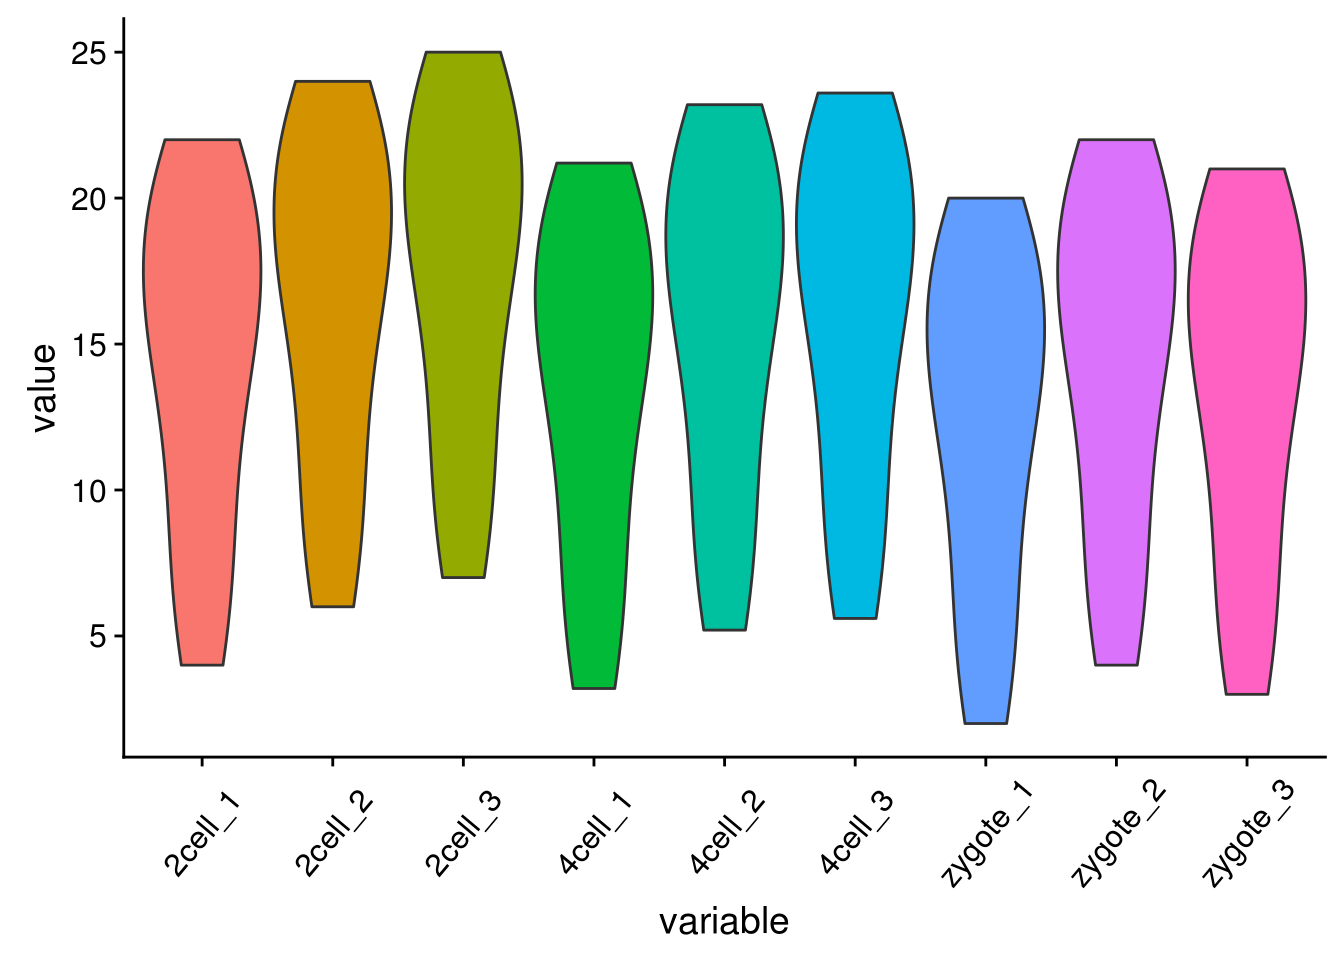
\includegraphics[width=0.95\linewidth,height=0.7\textheight,keepaspectratio]{R_course_files/figure-latex/unnamed-chunk-142-1} \end{center}

\begin{Shaded}
\begin{Highlighting}[]
\CommentTok{# variable和value为矩阵melt后的两列的名字,内部变量, variable代表了点线的属性,value代表对应的值。}
\NormalTok{p <-}\StringTok{ }\KeywordTok{ggplot}\NormalTok{(data_m, }\KeywordTok{aes}\NormalTok{(}\DataTypeTok{x=}\NormalTok{variable, }\DataTypeTok{y=}\NormalTok{value)) +}\StringTok{ }
\KeywordTok{geom_jitter}\NormalTok{(}\KeywordTok{aes}\NormalTok{(}\DataTypeTok{color=}\KeywordTok{factor}\NormalTok{(variable))) +}\StringTok{ }
\KeywordTok{theme}\NormalTok{(}\DataTypeTok{axis.text.x=}\KeywordTok{element_text}\NormalTok{(}\DataTypeTok{angle=}\DecValTok{50}\NormalTok{,}\DataTypeTok{hjust=}\FloatTok{0.5}\NormalTok{, }\DataTypeTok{vjust=}\FloatTok{0.5}\NormalTok{)) +}
\KeywordTok{theme}\NormalTok{(}\DataTypeTok{legend.position=}\StringTok{"none"}\NormalTok{)}
\NormalTok{p}
\CommentTok{# 图会存储在当前目录的Rplots.pdf文件中,如果用Rstudio,可以不运行dev.off()}
\CommentTok{#dev.off()}
\end{Highlighting}
\end{Shaded}

\begin{center}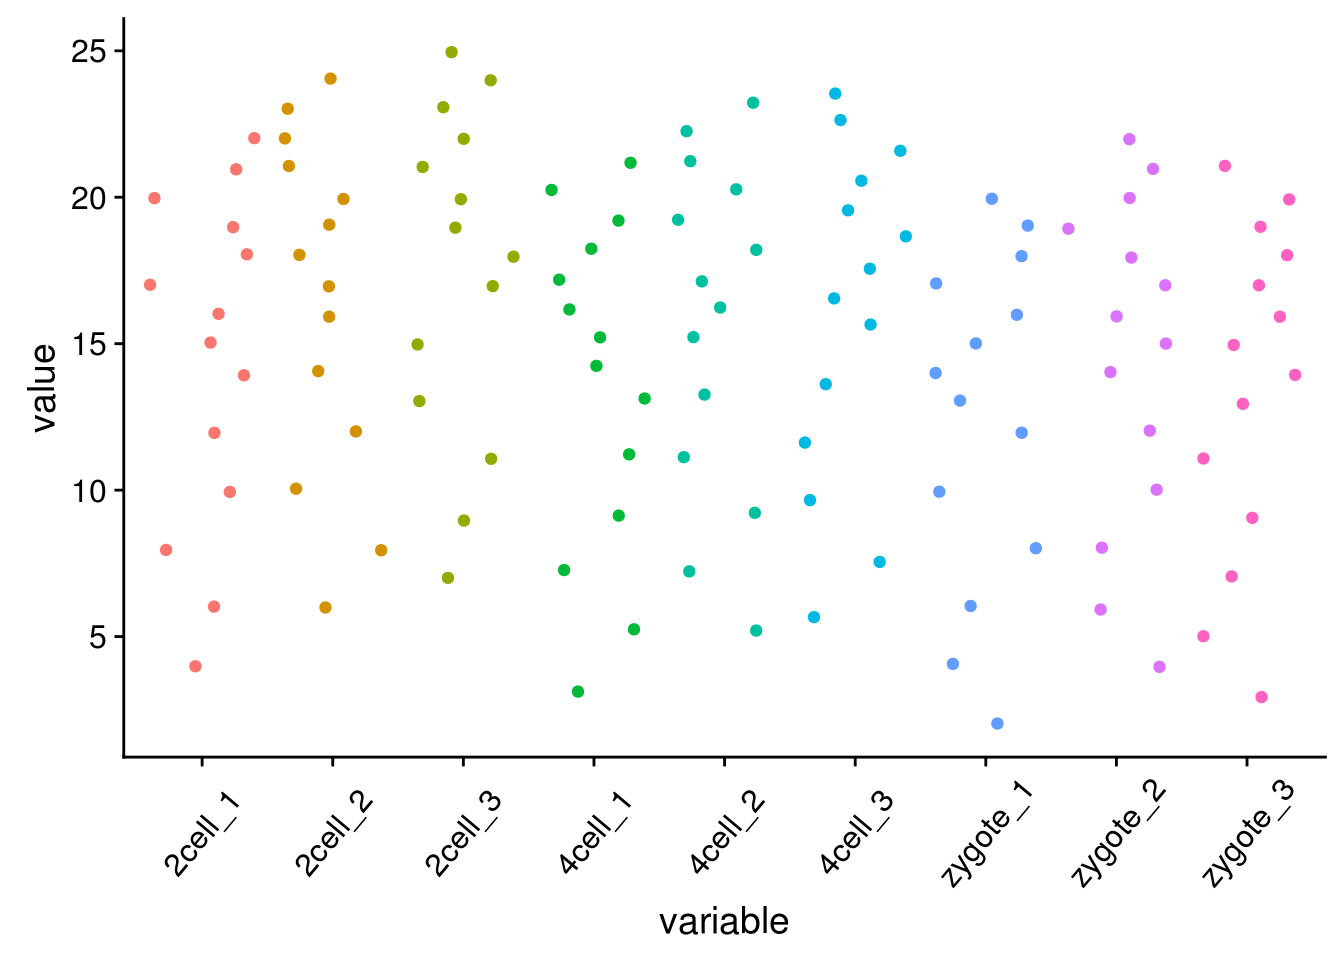
\includegraphics[width=0.95\linewidth,height=0.7\textheight,keepaspectratio]{R_course_files/figure-latex/unnamed-chunk-143-1} \end{center}

还有Jitter plot (这里使用的是ggbeeswarm包)

\begin{Shaded}
\begin{Highlighting}[]
\KeywordTok{library}\NormalTok{(ggbeeswarm)}
\CommentTok{# 为了更好的效果,只保留其中一个样品的数据}
\CommentTok{# grepl类似于Linux的grep命令,获取特定模式的字符串}

\NormalTok{data_m2 <-}\StringTok{ }\NormalTok{data_m[}\KeywordTok{grepl}\NormalTok{(}\StringTok{"_3"}\NormalTok{, data_m$variable),]}

\CommentTok{# variable和value为矩阵melt后的两列的名字,内部变量, }
\CommentTok{# variable代表了点线的属性,value代表对应的值。}
\NormalTok{p <-}\StringTok{ }\KeywordTok{ggplot}\NormalTok{(data_m2, }\KeywordTok{aes}\NormalTok{(}\DataTypeTok{x=}\NormalTok{variable, }\DataTypeTok{y=}\NormalTok{value),}\DataTypeTok{color=}\NormalTok{variable) +}\StringTok{ }
\KeywordTok{geom_quasirandom}\NormalTok{(}\KeywordTok{aes}\NormalTok{(}\DataTypeTok{colour=}\KeywordTok{factor}\NormalTok{(variable)), }\DataTypeTok{groupOnX=}\OtherTok{FALSE}\NormalTok{) +}\StringTok{ }
\KeywordTok{theme_bw}\NormalTok{() +}\StringTok{ }\KeywordTok{theme}\NormalTok{(}\DataTypeTok{panel.grid.major =} \KeywordTok{element_blank}\NormalTok{(),}
\DataTypeTok{panel.grid.minor =} \KeywordTok{element_blank}\NormalTok{(), }\DataTypeTok{legend.key=}\KeywordTok{element_blank}\NormalTok{()) +}
\KeywordTok{theme}\NormalTok{(}\DataTypeTok{legend.position=}\StringTok{"none"}\NormalTok{)}
\NormalTok{p}
\CommentTok{#ggsave(p, filename="jitterplot.pdf", width=14, height=8, units=c("cm"))}
\end{Highlighting}
\end{Shaded}

\begin{center}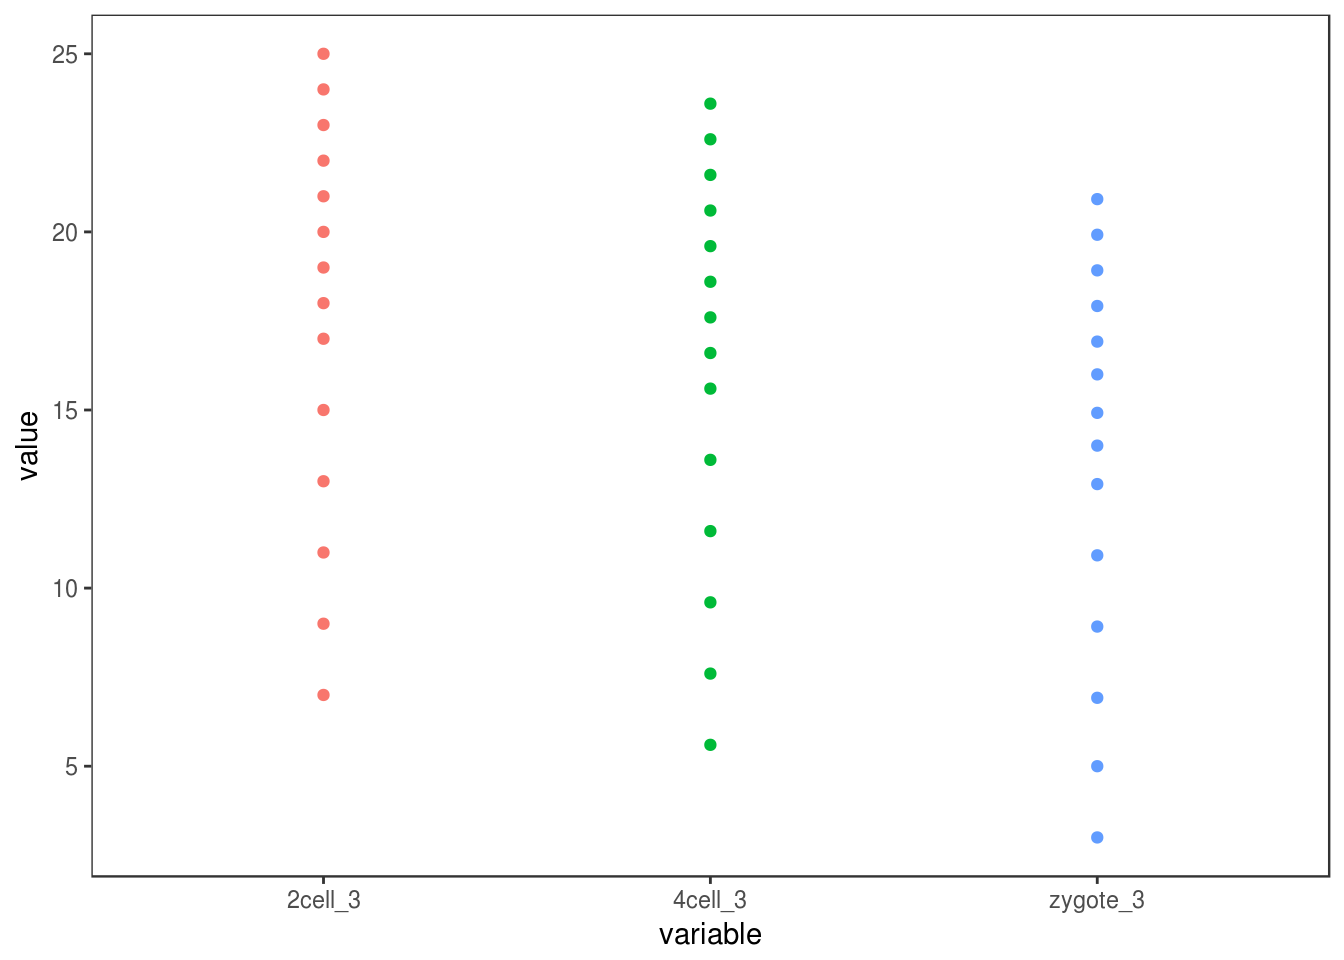
\includegraphics[width=0.95\linewidth,height=0.7\textheight,keepaspectratio]{R_course_files/figure-latex/unnamed-chunk-144-1} \end{center}

\begin{center}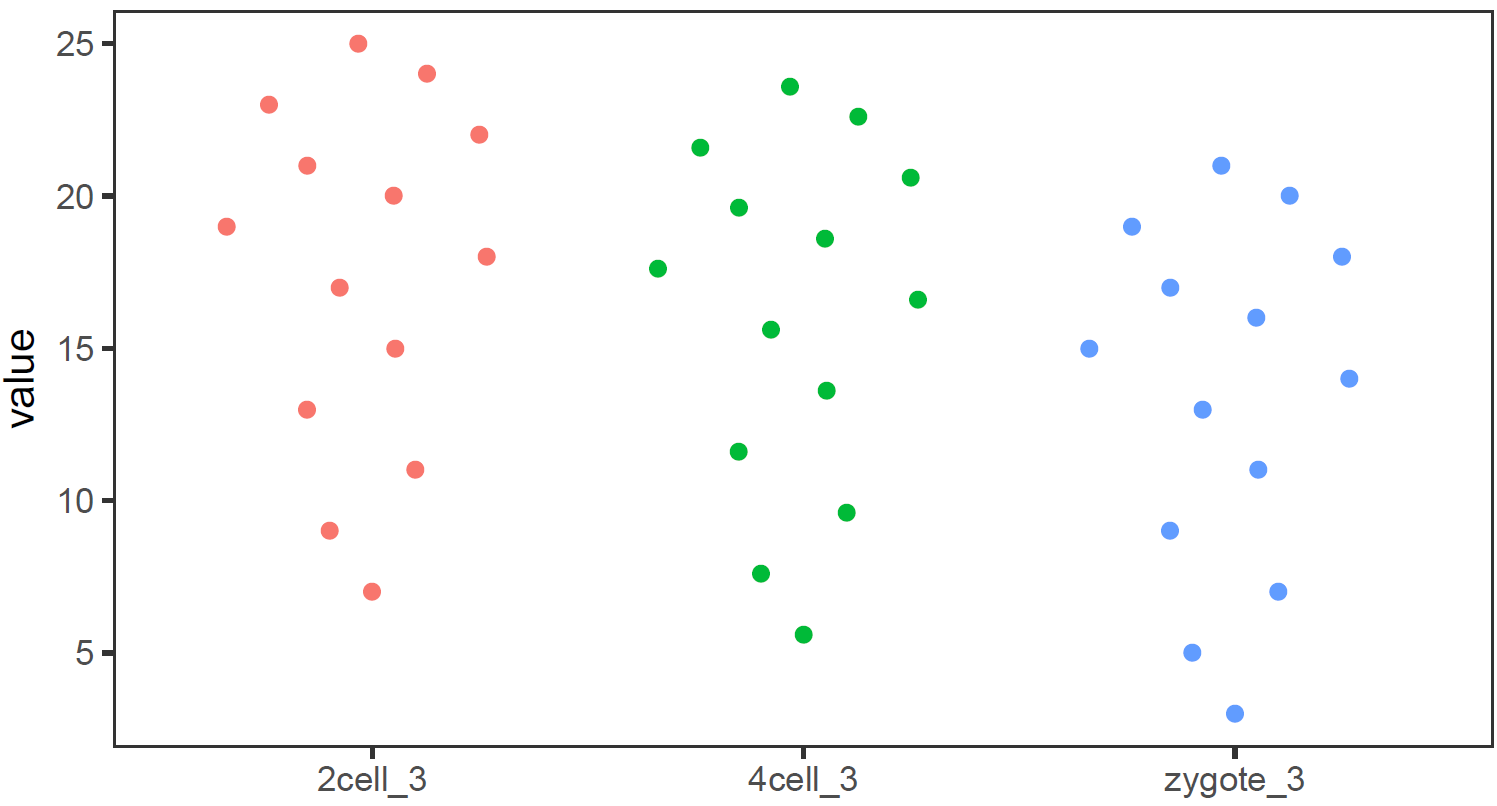
\includegraphics[width=0.95\linewidth,height=0.7\textheight,keepaspectratio]{images/boxplot_4} \end{center}

也可以用\texttt{geom\_jitter(aes(colour=factor(variable)))}代替\texttt{geom\_quasirandom(aes(colour=factor(variable)))}绘制抖动图,但个人认为geom\_quasirandom给出的结果更有特色。

\subsubsection{绘制单个基因 (A)的箱线图}\label{-a}

为了更好的展示效果,下面的矩阵增加了样品数量和样品的分组信息。

\begin{Shaded}
\begin{Highlighting}[]
\CommentTok{#profile="Name;2cell_1;2cell_2;2cell_3;2cell_4;2cell_5;2cell_6;4cell_1;4cell_2;4cell_3;\textbackslash{}}
\CommentTok{#4cell_4;4cell_5;4cell_6;zygote_1;zygote_2;zygote_3;zygote_4;zygote_5;zygote_6}
\CommentTok{#A;4;6;7;5;8;6;3.2;5.2;5.6;3.6;7.6;4.8;2;4;3;2;4;2.5}
\CommentTok{#B;6;8;9;7;10;8;5.2;7.2;7.6;5.6;9.6;6.8;4;6;5;4;6;4.5"}

\NormalTok{profile_text <-}\StringTok{ }\KeywordTok{read.table}\NormalTok{(}\StringTok{"data/boxplot_singleGene.data"}\NormalTok{, }\DataTypeTok{header=}\NormalTok{T, }\DataTypeTok{row.names=}\DecValTok{1}\NormalTok{, }\DataTypeTok{quote=}\StringTok{""}\NormalTok{, }
        \DataTypeTok{sep=}\StringTok{"}\CharTok{\textbackslash{}t}\StringTok{"}\NormalTok{, }\DataTypeTok{check.names=}\NormalTok{F)}

\NormalTok{data_m =}\StringTok{ }\KeywordTok{data.frame}\NormalTok{(}\KeywordTok{t}\NormalTok{(profile_text[}\StringTok{'A'}\NormalTok{,]))}
\NormalTok{data_m$sample =}\StringTok{ }\KeywordTok{rownames}\NormalTok{(data_m)}
\CommentTok{# 只挑选显示部分}
\CommentTok{# grepl前面已经讲过用于匹配}
\NormalTok{data_m[}\KeywordTok{grepl}\NormalTok{(}\StringTok{'_[123]'}\NormalTok{, data_m$sample),]}
\end{Highlighting}
\end{Shaded}

\begin{verbatim}
##            A   sample
## 2cell_1  4.0  2cell_1
## 2cell_2  6.0  2cell_2
## 2cell_3  7.0  2cell_3
## 4cell_1  3.2  4cell_1
## 4cell_2  5.2  4cell_2
## 4cell_3  5.6  4cell_3
## zygote_1 2.0 zygote_1
## zygote_2 4.0 zygote_2
## zygote_3 3.0 zygote_3
\end{verbatim}

获得样品分组信息
(这个例子比较特殊,样品的分组信息就是样品名字下划线前面的部分)

\begin{Shaded}
\begin{Highlighting}[]
\CommentTok{# 可以利用strsplit分割,取出其前面的字符串}
\CommentTok{# R中复杂的输出结果多数以列表的形式体现,在之前的矩阵操作教程中}
\CommentTok{# 提到过用str函数来查看复杂结果的结构,并从中获取信息}
\NormalTok{group =}\StringTok{ }\KeywordTok{unlist}\NormalTok{(}\KeywordTok{lapply}\NormalTok{(}\KeywordTok{strsplit}\NormalTok{(data_m$sample,}\StringTok{"_"}\NormalTok{), function(x) x[}\DecValTok{1}\NormalTok{]))}
\NormalTok{data_m$group =}\StringTok{ }\NormalTok{group}
\NormalTok{data_m[}\KeywordTok{grepl}\NormalTok{(}\StringTok{'_[123]'}\NormalTok{, data_m$sample),]}
\end{Highlighting}
\end{Shaded}

\begin{verbatim}
##            A   sample  group
## 2cell_1  4.0  2cell_1  2cell
## 2cell_2  6.0  2cell_2  2cell
## 2cell_3  7.0  2cell_3  2cell
## 4cell_1  3.2  4cell_1  4cell
## 4cell_2  5.2  4cell_2  4cell
## 4cell_3  5.6  4cell_3  4cell
## zygote_1 2.0 zygote_1 zygote
## zygote_2 4.0 zygote_2 zygote
## zygote_3 3.0 zygote_3 zygote
\end{verbatim}

如果没有这个规律,也可以提到类似于下面的文件,指定样品所属的组的信息。

\begin{Shaded}
\begin{Highlighting}[]
\NormalTok{sampleGroup_text=}\StringTok{"Sample;Group}
\StringTok{zygote_1;zygote}
\StringTok{zygote_2;zygote}
\StringTok{zygote_3;zygote}
\StringTok{zygote_4;zygote}
\StringTok{zygote_5;zygote}
\StringTok{zygote_6;zygote}
\StringTok{2cell_1;2cell}
\StringTok{2cell_2;2cell}
\StringTok{2cell_3;2cell}
\StringTok{2cell_4;2cell}
\StringTok{2cell_5;2cell}
\StringTok{2cell_6;2cell}
\StringTok{4cell_1;4cell}
\StringTok{4cell_2;4cell}
\StringTok{4cell_3;4cell}
\StringTok{4cell_4;4cell}
\StringTok{4cell_5;4cell}
\StringTok{4cell_6;4cell"}

\CommentTok{#sampleGroup = read.table(text=sampleGroup_text,sep="\textbackslash{}t",header=1,check.names=F,row.names=1)}

\CommentTok{#data_m <- merge(data_m, sampleGroup, by="row.names")}

\CommentTok{# 会获得相同的结果,脚本注释掉了以免重复执行引起问题。}
\end{Highlighting}
\end{Shaded}

矩阵准备好了,开始画图了 (小提琴图做例子,其它类似)

\begin{Shaded}
\begin{Highlighting}[]
\CommentTok{# 调整下样品出现的顺序}
\NormalTok{data_m$group <-}\StringTok{ }\KeywordTok{factor}\NormalTok{(data_m$group, }\DataTypeTok{levels=}\KeywordTok{c}\NormalTok{(}\StringTok{"zygote"}\NormalTok{,}\StringTok{"2cell"}\NormalTok{,}\StringTok{"4cell"}\NormalTok{))}
\CommentTok{# group和A为矩阵中两列的名字,group代表了值的属性,A代表基因A对应的表达值。}
\CommentTok{# 注意看修改了的地方}
\NormalTok{p <-}\StringTok{ }\KeywordTok{ggplot}\NormalTok{(data_m, }\KeywordTok{aes}\NormalTok{(}\DataTypeTok{x=}\NormalTok{group, }\DataTypeTok{y=}\NormalTok{A)) +}\StringTok{ }
\StringTok{  }\KeywordTok{geom_violin}\NormalTok{(}\KeywordTok{aes}\NormalTok{(}\DataTypeTok{fill=}\KeywordTok{factor}\NormalTok{(group))) +}\StringTok{ }
\StringTok{  }\KeywordTok{theme}\NormalTok{(}\DataTypeTok{axis.text.x=}\KeywordTok{element_text}\NormalTok{(}\DataTypeTok{angle=}\DecValTok{50}\NormalTok{,}\DataTypeTok{hjust=}\FloatTok{0.5}\NormalTok{, }\DataTypeTok{vjust=}\FloatTok{0.5}\NormalTok{)) +}
\StringTok{  }\KeywordTok{theme}\NormalTok{(}\DataTypeTok{legend.position=}\StringTok{"none"}\NormalTok{)}
\NormalTok{p}
\CommentTok{# 图会存储在当前目录的Rplots.pdf文件中,如果用Rstudio,可以不运行dev.off()}
\CommentTok{#dev.off()}
\end{Highlighting}
\end{Shaded}

\begin{center}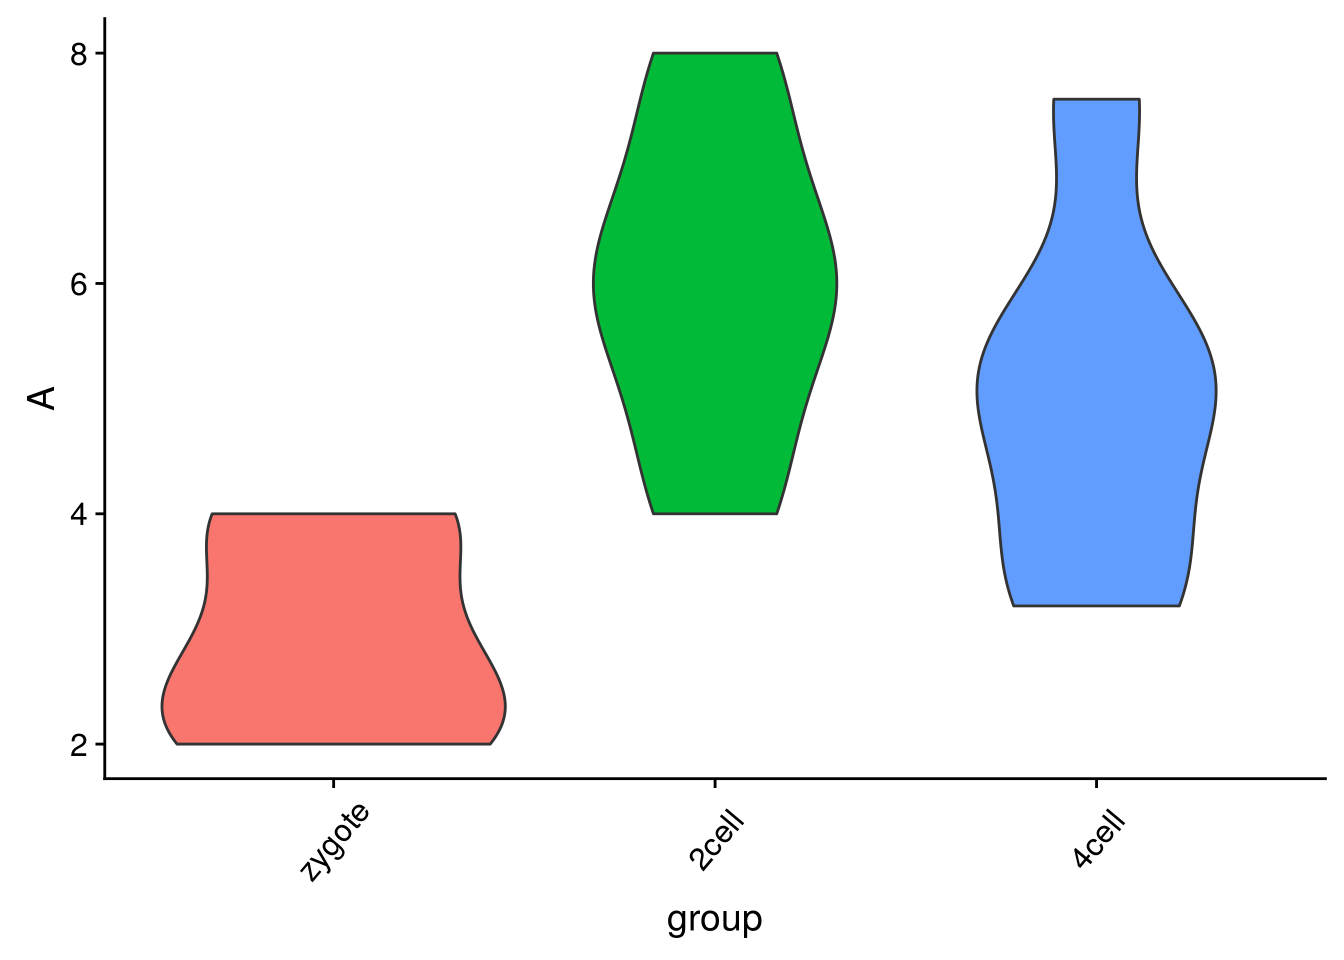
\includegraphics[width=0.95\linewidth,height=0.7\textheight,keepaspectratio]{R_course_files/figure-latex/unnamed-chunk-149-1} \end{center}

\subsubsection{长矩阵绘制箱线图}

常规矩阵绘制箱线图要求必须是个方正的矩阵输入,而有时想比较的几个组里面检测的值数目不同。比如有三个组,GrpA组检测了6个病人,GrpB组检测了10个病人,GrpC组是12个正常人的检测数据。这时就很难形成一个行为检测值,列为样品的矩阵,就需要长表格模式解决这一问题。

\begin{Shaded}
\begin{Highlighting}[]
\NormalTok{long_table <-}\StringTok{ "Grp;Value}
\StringTok{GrpA;10}
\StringTok{GrpA;11}
\StringTok{GrpA;11}
\StringTok{GrpA;11}
\StringTok{GrpA;12}
\StringTok{GrpA;11}
\StringTok{GrpA;15}
\StringTok{GrpB;5}
\StringTok{GrpB;4}
\StringTok{GrpB;3}
\StringTok{GrpB;2}
\StringTok{GrpB;4}
\StringTok{GrpB;3}
\StringTok{GrpB;2}
\StringTok{GrpB;3}
\StringTok{GrpB;3.1}
\StringTok{GrpC;2}
\StringTok{GrpC;1}
\StringTok{GrpC;1}
\StringTok{GrpC;1.1}
\StringTok{GrpC;1.5}
\StringTok{GrpC;1.1}
\StringTok{GrpC;1.5}
\StringTok{GrpC;1.8}
\StringTok{GrpC;2"}

\NormalTok{long_table <-}\StringTok{ }\KeywordTok{read.table}\NormalTok{(}\DataTypeTok{text=}\NormalTok{long_table,}\DataTypeTok{sep=}\StringTok{";"}\NormalTok{,}\DataTypeTok{header=}\NormalTok{T,}\DataTypeTok{check.names=}\NormalTok{F)}

\NormalTok{p <-}\StringTok{ }\KeywordTok{ggplot}\NormalTok{(long_table, }\KeywordTok{aes}\NormalTok{(}\DataTypeTok{x=}\NormalTok{Grp, }\DataTypeTok{y=}\NormalTok{Value)) +}\StringTok{ }
\KeywordTok{geom_violin}\NormalTok{(}\KeywordTok{aes}\NormalTok{(}\DataTypeTok{fill=}\KeywordTok{factor}\NormalTok{(Grp))) +}\StringTok{ }
\KeywordTok{theme}\NormalTok{(}\DataTypeTok{axis.text.x=}\KeywordTok{element_text}\NormalTok{(}\DataTypeTok{angle=}\DecValTok{50}\NormalTok{,}\DataTypeTok{hjust=}\FloatTok{0.5}\NormalTok{, }\DataTypeTok{vjust=}\FloatTok{0.5}\NormalTok{)) +}
\KeywordTok{theme}\NormalTok{(}\DataTypeTok{legend.position=}\StringTok{"none"}\NormalTok{)}
\NormalTok{p}
\end{Highlighting}
\end{Shaded}

\begin{center}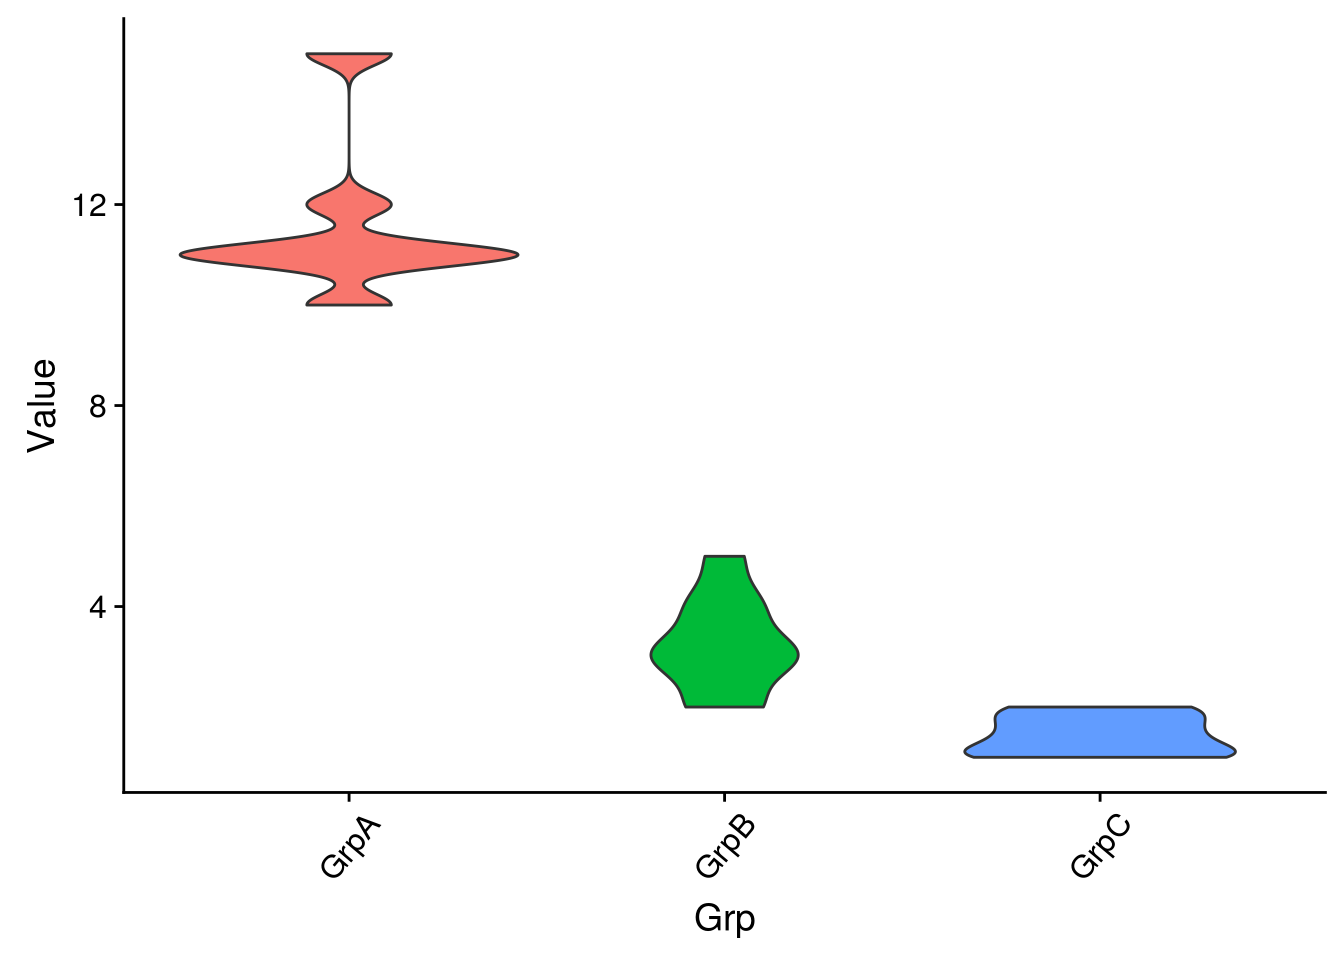
\includegraphics[width=0.95\linewidth,height=0.7\textheight,keepaspectratio]{R_course_files/figure-latex/unnamed-chunk-150-1} \end{center}

\begin{Shaded}
\begin{Highlighting}[]
\NormalTok{a =}\StringTok{ }\KeywordTok{c}\NormalTok{(}\KeywordTok{rep}\NormalTok{(}\KeywordTok{c}\NormalTok{(}\StringTok{'F'}\NormalTok{,}\StringTok{"M"}\NormalTok{),}\DecValTok{12}\NormalTok{), }\StringTok{'F'}\NormalTok{)}
\NormalTok{long_table$gender <-}\StringTok{ }\NormalTok{a}

\NormalTok{p <-}\StringTok{ }\KeywordTok{ggplot}\NormalTok{(long_table, }\KeywordTok{aes}\NormalTok{(}\DataTypeTok{x=}\NormalTok{Grp, }\DataTypeTok{y=}\NormalTok{Value)) +}\StringTok{ }
\StringTok{  }\KeywordTok{geom_boxplot}\NormalTok{(}\KeywordTok{aes}\NormalTok{(}\DataTypeTok{fill=}\KeywordTok{factor}\NormalTok{(gender))) +}
\StringTok{  }\KeywordTok{geom_quasirandom}\NormalTok{(}\DataTypeTok{groupOnX=}\OtherTok{FALSE}\NormalTok{)}
\NormalTok{p}
\end{Highlighting}
\end{Shaded}

\begin{center}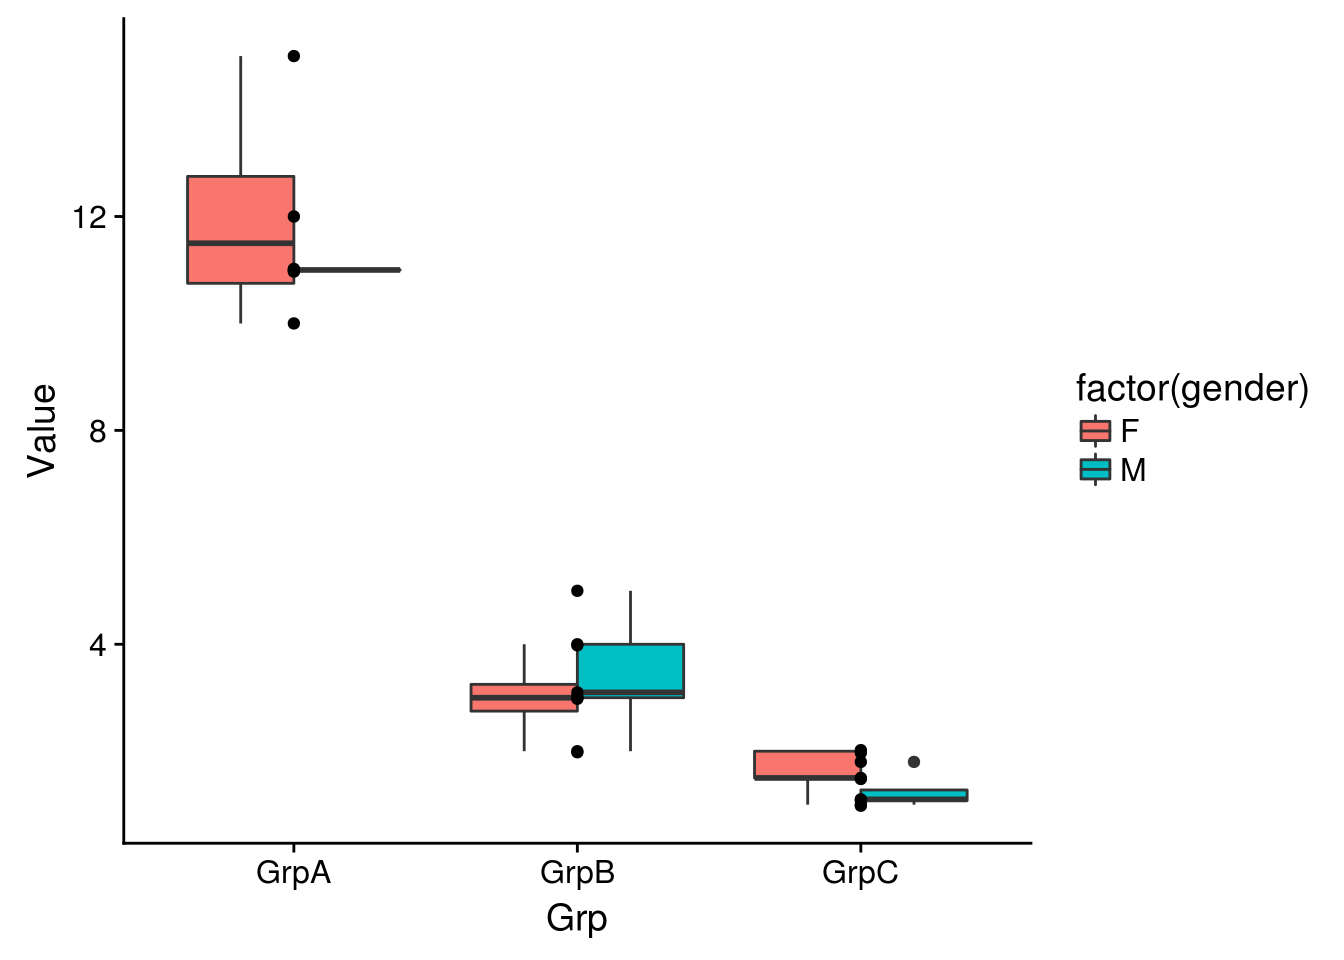
\includegraphics[width=0.95\linewidth,height=0.7\textheight,keepaspectratio]{R_course_files/figure-latex/unnamed-chunk-151-1} \end{center}

长表格形式自身就是常规矩阵melt后的格式,这种用来绘制箱线图就很简单了,就不举例子了。

\subsection{线图}

线图是反映趋势变化的一种方式,其输入数据一般也是一个矩阵。

\subsubsection{单线图}

假设有这么一个矩阵,第一列为转录起始位点及其上下游\texttt{5\ kb}的区域,第二列为\texttt{H3K27ac}修饰在这些区域的丰度,想绘制一张线图展示。

\begin{Shaded}
\begin{Highlighting}[]
\NormalTok{profile=}\StringTok{"Pos;H3K27ac}
\StringTok{-5000;8.7}
\StringTok{-4000;8.4}
\StringTok{-3000;8.3}
\StringTok{-2000;7.2}
\StringTok{-1000;3.6}
\StringTok{0;3.6}
\StringTok{1000;7.1}
\StringTok{2000;8.2}
\StringTok{3000;8.4}
\StringTok{4000;8.5}
\StringTok{5000;8.5"}
\end{Highlighting}
\end{Shaded}

读入数据

\begin{Shaded}
\begin{Highlighting}[]
\NormalTok{profile_text <-}\StringTok{ }\KeywordTok{read.table}\NormalTok{(}\DataTypeTok{text=}\NormalTok{profile, }\DataTypeTok{header=}\NormalTok{T, }\DataTypeTok{row.names=}\OtherTok{NULL}\NormalTok{, }\DataTypeTok{quote=}\StringTok{""}\NormalTok{,}\DataTypeTok{sep=}\StringTok{";"}\NormalTok{)}
\NormalTok{profile_text}
\end{Highlighting}
\end{Shaded}

\begin{verbatim}
##      Pos H3K27ac
## 1  -5000     8.7
## 2  -4000     8.4
## 3  -3000     8.3
## 4  -2000     7.2
## 5  -1000     3.6
## 6      0     3.6
## 7   1000     7.1
## 8   2000     8.2
## 9   3000     8.4
## 10  4000     8.5
## 11  5000     8.5
\end{verbatim}

\begin{Shaded}
\begin{Highlighting}[]
\KeywordTok{plot}\NormalTok{(profile_text$Pos, profile_text$H3K27ac,}\DataTypeTok{type =} \StringTok{"l"}\NormalTok{)}
\end{Highlighting}
\end{Shaded}

\begin{center}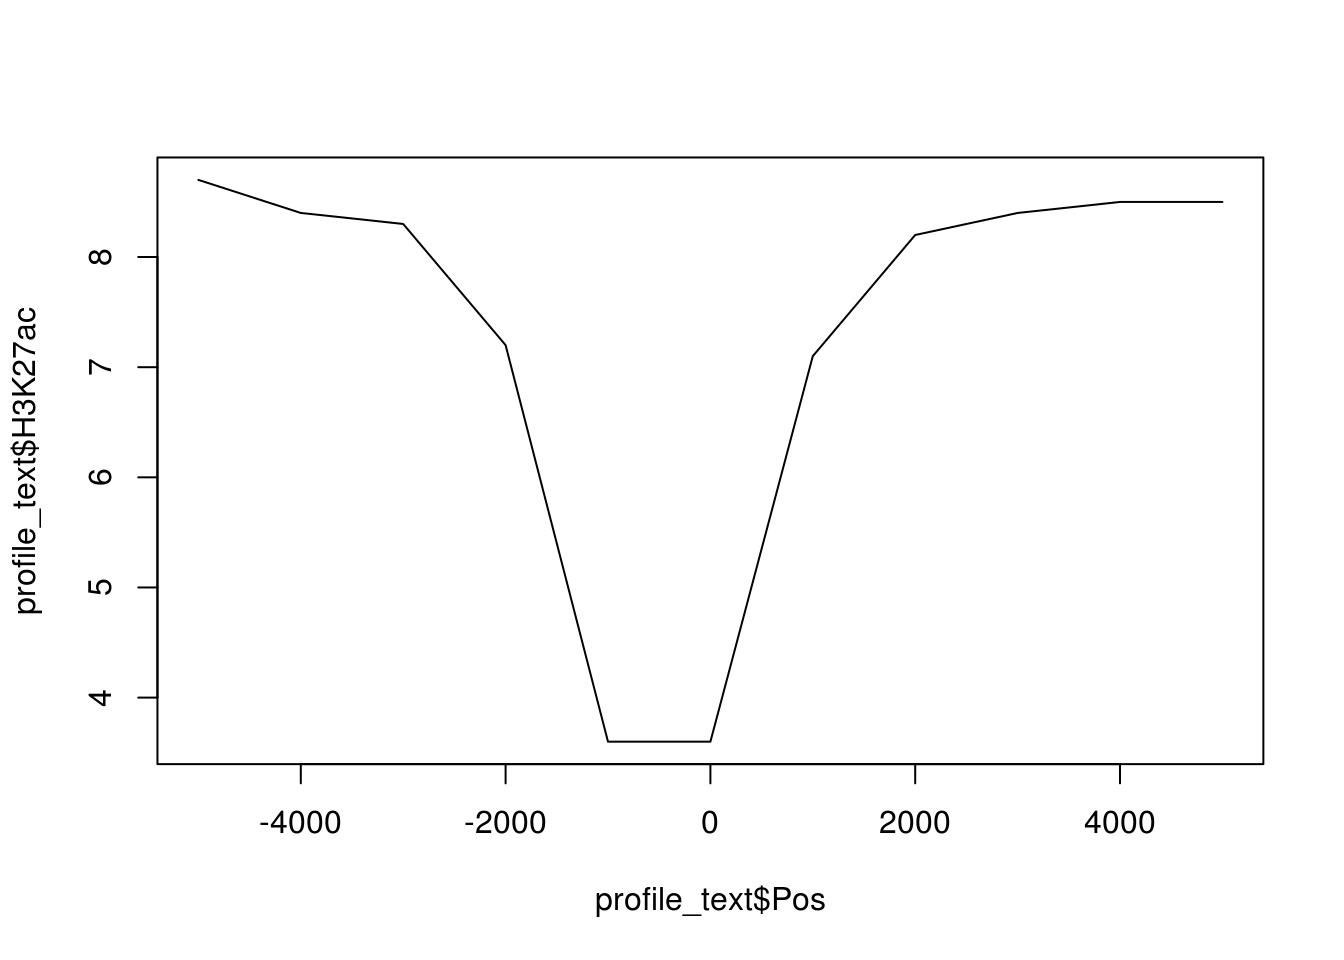
\includegraphics[width=0.95\linewidth,height=0.7\textheight,keepaspectratio]{R_course_files/figure-latex/unnamed-chunk-154-1} \end{center}

\begin{Shaded}
\begin{Highlighting}[]
\KeywordTok{ggplot}\NormalTok{(profile_text, }\KeywordTok{aes}\NormalTok{(}\DataTypeTok{x=}\NormalTok{Pos, }\DataTypeTok{y=}\NormalTok{H3K27ac)) +}\StringTok{ }\KeywordTok{geom_line}\NormalTok{()}
\end{Highlighting}
\end{Shaded}

\begin{center}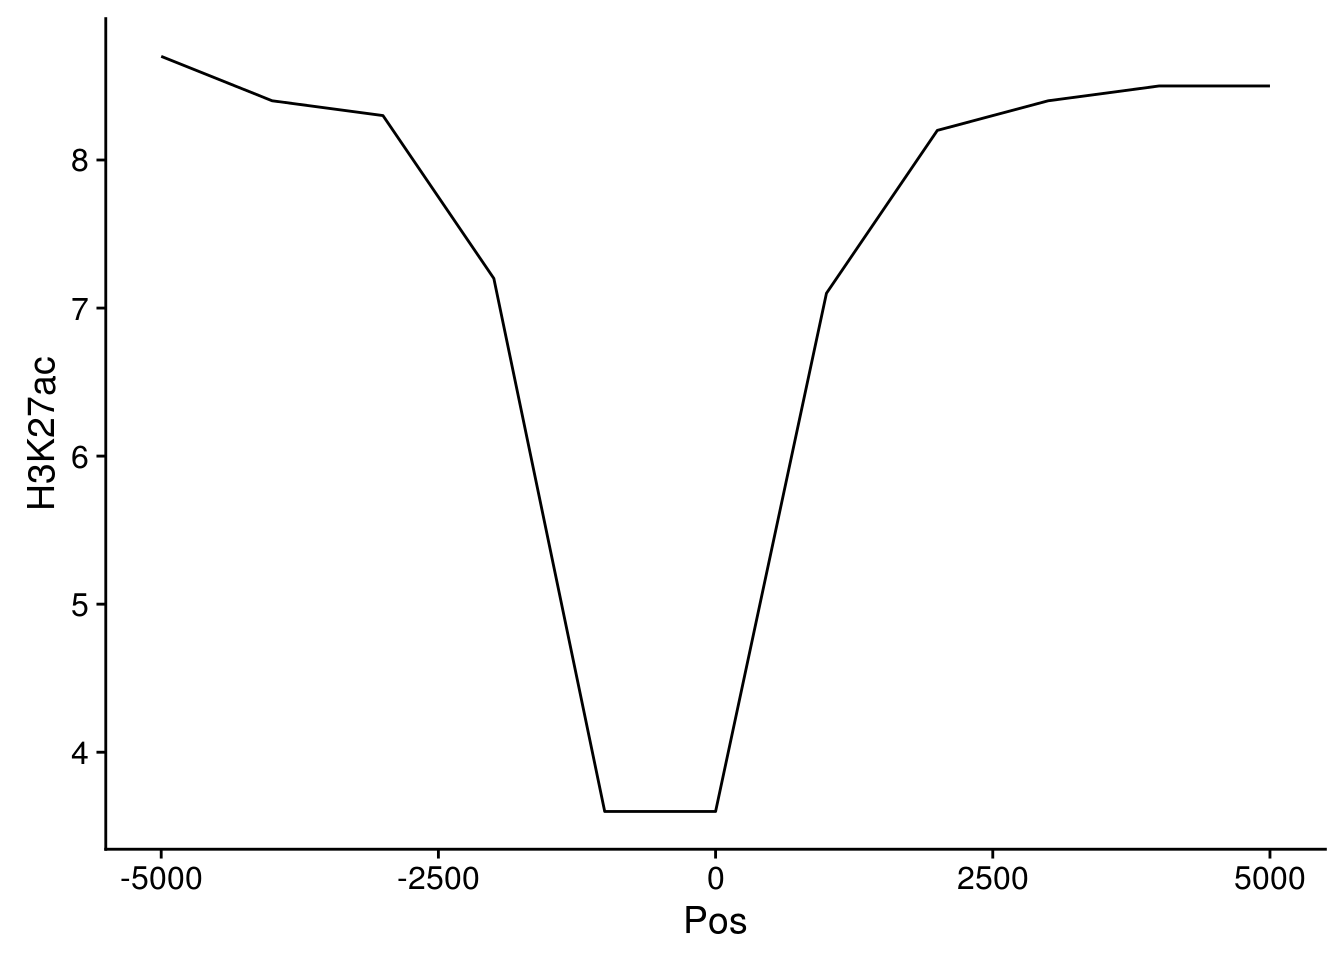
\includegraphics[width=0.95\linewidth,height=0.7\textheight,keepaspectratio]{R_course_files/figure-latex/unnamed-chunk-155-1} \end{center}

\begin{Shaded}
\begin{Highlighting}[]
\NormalTok{profile_text <-}\StringTok{ }\KeywordTok{read.table}\NormalTok{(}\DataTypeTok{text=}\NormalTok{profile, }\DataTypeTok{header=}\NormalTok{T, }\DataTypeTok{row.names=}\DecValTok{1}\NormalTok{, }\DataTypeTok{quote=}\StringTok{""}\NormalTok{,}\DataTypeTok{sep=}\StringTok{";"}\NormalTok{)}
\NormalTok{profile_text}
\end{Highlighting}
\end{Shaded}

\begin{verbatim}
##       H3K27ac
## -5000     8.7
## -4000     8.4
## -3000     8.3
## -2000     7.2
## -1000     3.6
## 0         3.6
## 1000      7.1
## 2000      8.2
## 3000      8.4
## 4000      8.5
## 5000      8.5
\end{verbatim}

\begin{Shaded}
\begin{Highlighting}[]
\CommentTok{# 在melt时保留位置信息}
\CommentTok{# melt格式是ggplot2画图最喜欢的格式}
\CommentTok{# 好好体会下这个格式,虽然多占用了不少空间,但是确实很方便}

\CommentTok{# 这里可以用 `xvariable`,也可以是其它字符串,但需要保证后面与这里的一致}
\CommentTok{# 因为这一列是要在X轴显示,所以起名为`xvariable`。}
\NormalTok{profile_text$xvariable =}\StringTok{ }\KeywordTok{rownames}\NormalTok{(profile_text)}
\CommentTok{#library(ggplot2)}
\CommentTok{#library(reshape2)}
\NormalTok{data_m <-}\StringTok{ }\KeywordTok{melt}\NormalTok{(profile_text, }\DataTypeTok{id.vars=}\KeywordTok{c}\NormalTok{(}\StringTok{"xvariable"}\NormalTok{))}
\NormalTok{data_m}
\end{Highlighting}
\end{Shaded}

\begin{verbatim}
##    xvariable variable value
## 1      -5000  H3K27ac   8.7
## 2      -4000  H3K27ac   8.4
## 3      -3000  H3K27ac   8.3
## 4      -2000  H3K27ac   7.2
## 5      -1000  H3K27ac   3.6
## 6          0  H3K27ac   3.6
## 7       1000  H3K27ac   7.1
## 8       2000  H3K27ac   8.2
## 9       3000  H3K27ac   8.4
## 10      4000  H3K27ac   8.5
## 11      5000  H3K27ac   8.5
\end{verbatim}

然后开始画图,与上面画heatmap一样。

\begin{Shaded}
\begin{Highlighting}[]
\CommentTok{# variable和value为矩阵melt后的两列的名字,内部变量, variable代表了点线的属性,value代表对应的值。}
\NormalTok{p <-}\StringTok{ }\KeywordTok{ggplot}\NormalTok{(data_m, }\KeywordTok{aes}\NormalTok{(}\DataTypeTok{x=}\NormalTok{xvariable, }\DataTypeTok{y=}\NormalTok{value,}\DataTypeTok{color=}\NormalTok{variable)) +}\StringTok{ }\KeywordTok{geom_line}\NormalTok{()}
\NormalTok{p}
\end{Highlighting}
\end{Shaded}

\begin{verbatim}
## geom_path: Each group consists of only one observation. Do you need to
## adjust the group aesthetic?
\end{verbatim}

\begin{Shaded}
\begin{Highlighting}[]
\CommentTok{# 图会存储在当前目录的Rplots.pdf文件中,如果用Rstudio,可以不运行dev.off()}
\CommentTok{# dev.off()}
\end{Highlighting}
\end{Shaded}

\begin{center}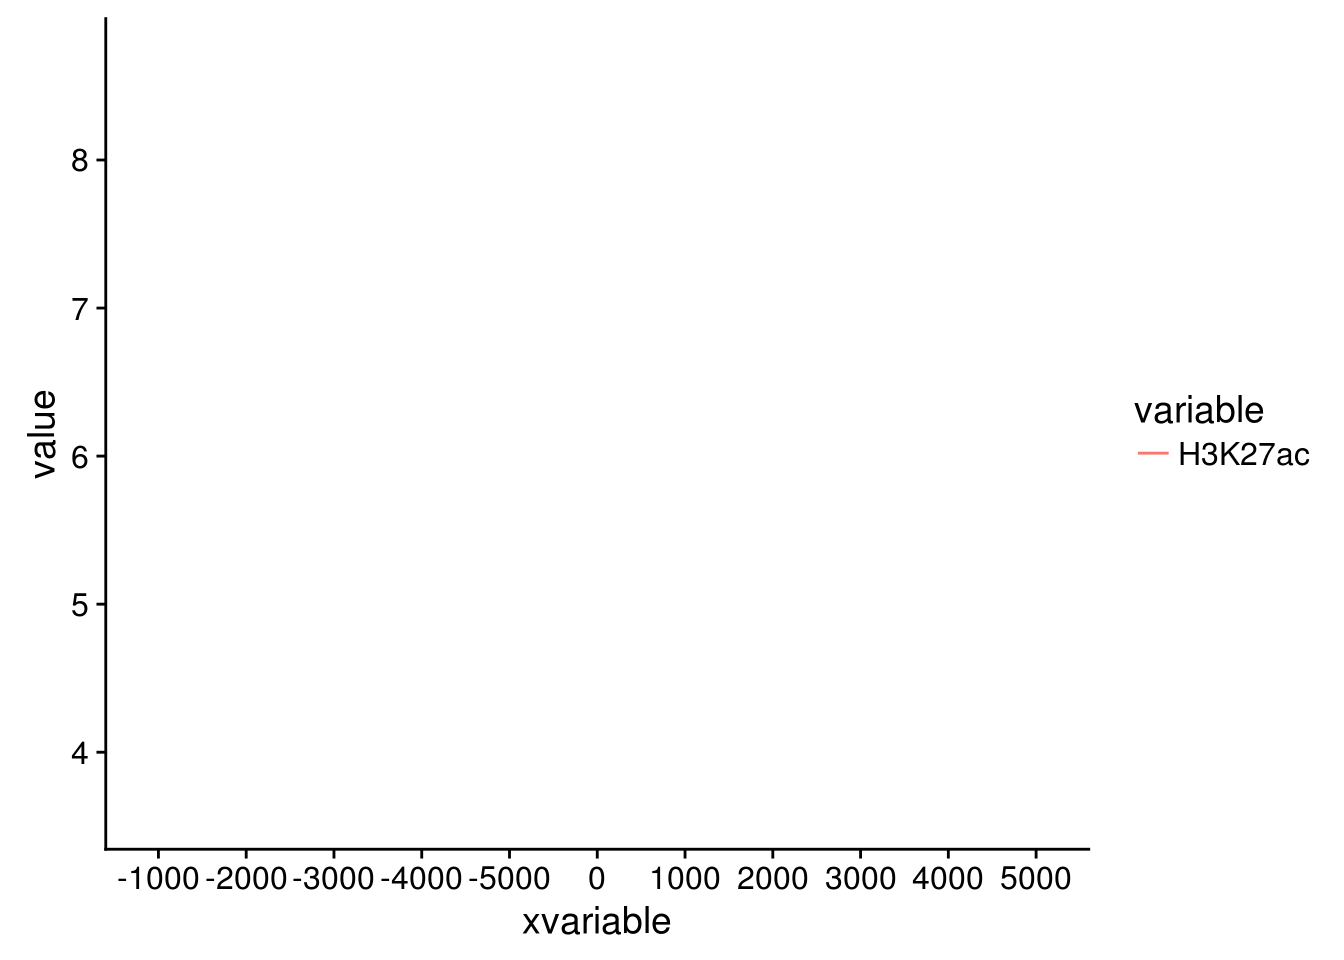
\includegraphics[width=0.95\linewidth,height=0.7\textheight,keepaspectratio]{R_course_files/figure-latex/unnamed-chunk-158-1} \end{center}

满心期待一个倒钟形曲线,结果,什么也没有。

仔细看,出来一段提示

\begin{verbatim}
geom_path: Each group consists of only one observation. 
Do you need to adjust the group aesthetic?
\end{verbatim}

原来默认ggplot2把每个点都视作了一个分组,什么都没画出来。而\texttt{data\_m}中的数据都来源于一个分组\texttt{H3K27ac},分组的名字为\texttt{variable},修改下脚本,看看效果。

\begin{Shaded}
\begin{Highlighting}[]
\NormalTok{p <-}\StringTok{ }\KeywordTok{ggplot}\NormalTok{(data_m, }\KeywordTok{aes}\NormalTok{(}\DataTypeTok{x=}\NormalTok{xvariable, }\DataTypeTok{y=}\NormalTok{value,}\DataTypeTok{color=}\NormalTok{variable,}\DataTypeTok{group=}\NormalTok{variable)) +}\StringTok{ }
\StringTok{     }\KeywordTok{geom_line}\NormalTok{() +}\StringTok{ }\KeywordTok{theme}\NormalTok{(}\DataTypeTok{legend.position=}\KeywordTok{c}\NormalTok{(}\FloatTok{0.1}\NormalTok{,}\FloatTok{0.9}\NormalTok{))}
\NormalTok{p}
\CommentTok{# dev.off()}
\end{Highlighting}
\end{Shaded}

\begin{center}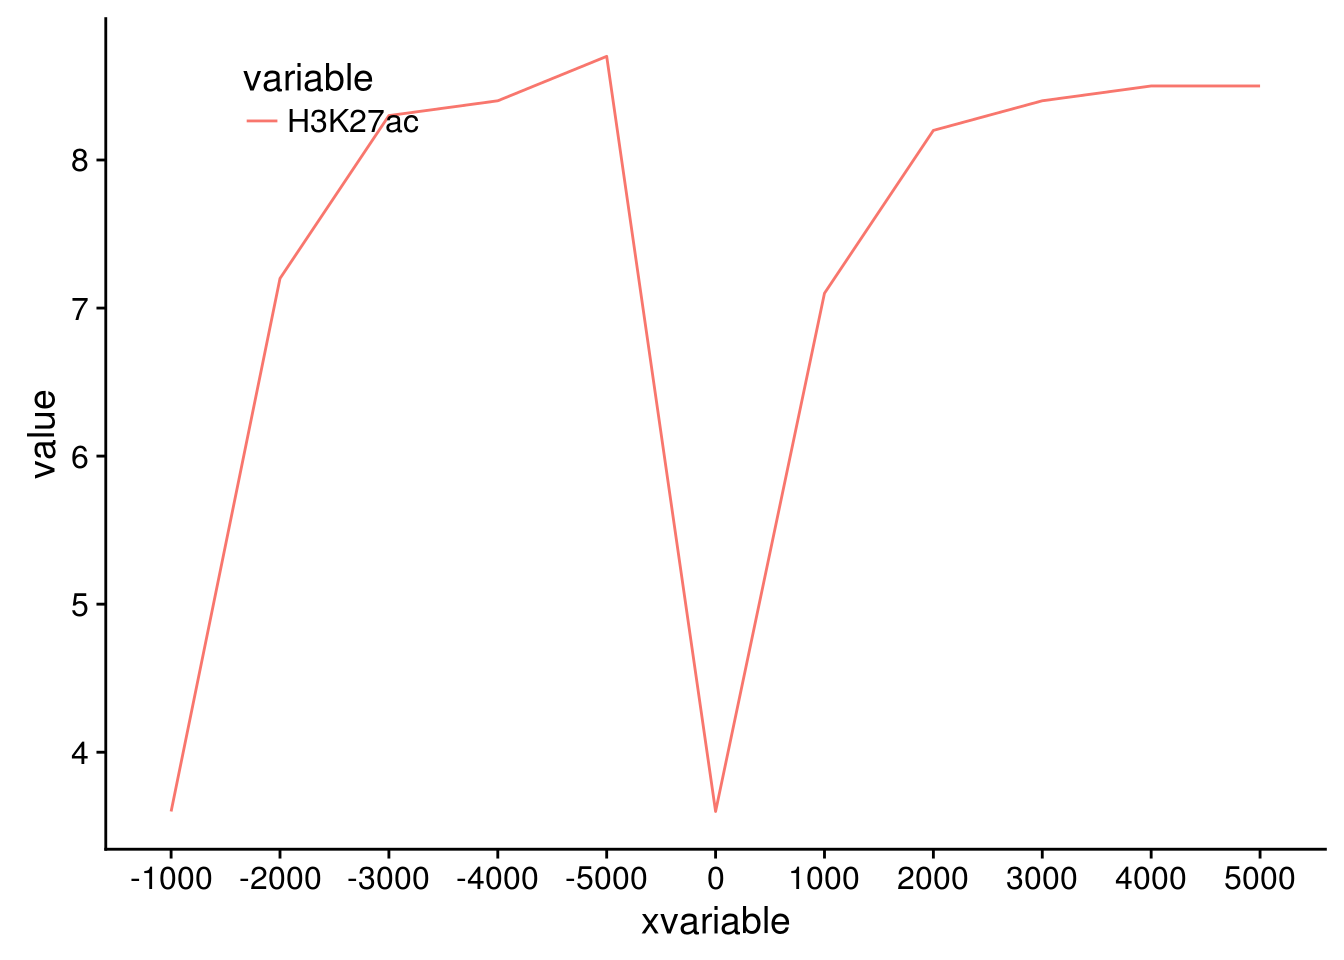
\includegraphics[width=0.95\linewidth,height=0.7\textheight,keepaspectratio]{R_course_files/figure-latex/unnamed-chunk-159-1} \end{center}

图出来了,一条线,看一眼没问题;再仔细看,不对了,怎么还不是倒钟形,原来横坐标错位了。

检查下数据格式

\begin{Shaded}
\begin{Highlighting}[]
\KeywordTok{summary}\NormalTok{(data_m)}
\end{Highlighting}
\end{Shaded}

\begin{verbatim}
##   xvariable            variable      value      
##  Length:11          H3K27ac:11   Min.   :3.600  
##  Class :character                1st Qu.:7.150  
##  Mode  :character                Median :8.300  
##                                  Mean   :7.318  
##                                  3rd Qu.:8.450  
##                                  Max.   :8.700
\end{verbatim}

问题来了,\texttt{xvariable}虽然看上去数字,但存储的实际是字符串
(因为是作为行名字读取的),需要转换为数字。

\begin{Shaded}
\begin{Highlighting}[]
\NormalTok{data_m$xvariable <-}\StringTok{ }\KeywordTok{as.numeric}\NormalTok{(data_m$xvariable)}

\CommentTok{#再检验下}
\KeywordTok{summary}\NormalTok{(data_m)}
\end{Highlighting}
\end{Shaded}

\begin{verbatim}
##    xvariable        variable      value      
##  Min.   :-5000   H3K27ac:11   Min.   :3.600  
##  1st Qu.:-2500                1st Qu.:7.150  
##  Median :    0                Median :8.300  
##  Mean   :    0                Mean   :7.318  
##  3rd Qu.: 2500                3rd Qu.:8.450  
##  Max.   : 5000                Max.   :8.700
\end{verbatim}

好了,继续画图。

\begin{Shaded}
\begin{Highlighting}[]
\CommentTok{# 注意断行时,加号在行尾,不能放在行首}
\NormalTok{p <-}\StringTok{ }\KeywordTok{ggplot}\NormalTok{(data_m, }\KeywordTok{aes}\NormalTok{(}\DataTypeTok{x=}\NormalTok{xvariable, }\DataTypeTok{y=}\NormalTok{value,}\DataTypeTok{color=}\NormalTok{variable,}\DataTypeTok{group=}\NormalTok{variable)) +}
\StringTok{     }\KeywordTok{geom_line}\NormalTok{() +}\StringTok{ }\KeywordTok{theme}\NormalTok{(}\DataTypeTok{legend.position=}\KeywordTok{c}\NormalTok{(}\FloatTok{0.07}\NormalTok{,}\FloatTok{0.7}\NormalTok{))}
\NormalTok{p}
\CommentTok{#dev.off()}
\end{Highlighting}
\end{Shaded}

\begin{center}\includegraphics[width=0.95\linewidth,height=0.7\textheight,keepaspectratio]{R_course_files/figure-latex/unnamed-chunk-162-1} \end{center}

图终于出来了,调了下legend的位置,看上去有点意思了。

有点难看,如果平滑下,会不会好一些,\texttt{stat\_smooth}可以对绘制的线进行局部拟合。在不影响变化趋势的情况下,可以使用
(但慎用)。

\begin{Shaded}
\begin{Highlighting}[]
\NormalTok{p <-}\StringTok{ }\KeywordTok{ggplot}\NormalTok{(data_m, }\KeywordTok{aes}\NormalTok{(}\DataTypeTok{x=}\NormalTok{xvariable, }\DataTypeTok{y=}\NormalTok{value,}\DataTypeTok{color=}\NormalTok{variable,}\DataTypeTok{group=}\NormalTok{variable)) +}\StringTok{ }
\StringTok{     }\KeywordTok{geom_line}\NormalTok{() +}\StringTok{ }\KeywordTok{stat_smooth}\NormalTok{(}\DataTypeTok{method=}\StringTok{"auto"}\NormalTok{, }\DataTypeTok{se=}\OtherTok{FALSE}\NormalTok{) +}\StringTok{ }
\StringTok{     }\KeywordTok{theme}\NormalTok{(}\DataTypeTok{legend.position=}\KeywordTok{c}\NormalTok{(}\FloatTok{0.06}\NormalTok{,}\FloatTok{0.5}\NormalTok{))}
\NormalTok{p}
\end{Highlighting}
\end{Shaded}

\begin{verbatim}
## `geom_smooth()` using method = 'loess'
\end{verbatim}

\begin{Shaded}
\begin{Highlighting}[]
\CommentTok{#dev.off()}
\end{Highlighting}
\end{Shaded}

\begin{center}\includegraphics[width=0.95\linewidth,height=0.7\textheight,keepaspectratio]{R_course_files/figure-latex/unnamed-chunk-163-1} \end{center}

从图中看,趋势还是一致的,线条更优美了。另外一个方式是增加区间的数量,线也会好些,而且更真实。

\texttt{stat\_smooth}和\texttt{geom\_line}各绘制了一条线,只保留一条就好。

\begin{Shaded}
\begin{Highlighting}[]
\NormalTok{p <-}\StringTok{ }\KeywordTok{ggplot}\NormalTok{(data_m, }\KeywordTok{aes}\NormalTok{(}\DataTypeTok{x=}\NormalTok{xvariable, }\DataTypeTok{y=}\NormalTok{value,}\DataTypeTok{color=}\NormalTok{variable,}\DataTypeTok{group=}\NormalTok{variable)) +}\StringTok{ }
\StringTok{     }\KeywordTok{stat_smooth}\NormalTok{(}\DataTypeTok{method=}\StringTok{"auto"}\NormalTok{, }\DataTypeTok{se=}\OtherTok{FALSE}\NormalTok{) +}\StringTok{ }\KeywordTok{theme}\NormalTok{(}\DataTypeTok{legend.position=}\KeywordTok{c}\NormalTok{(}\FloatTok{0.06}\NormalTok{,}\FloatTok{0.5}\NormalTok{))}
\NormalTok{p}
\end{Highlighting}
\end{Shaded}

\begin{verbatim}
## `geom_smooth()` using method = 'loess'
\end{verbatim}

\begin{Shaded}
\begin{Highlighting}[]
\CommentTok{#dev.off()}
\end{Highlighting}
\end{Shaded}

\begin{center}\includegraphics[width=0.95\linewidth,height=0.7\textheight,keepaspectratio]{R_course_files/figure-latex/unnamed-chunk-164-1} \end{center}

好了,终于完成了单条线图的绘制。

\subsubsection{多线图}

那么再来一个多线图的例子吧,只要给之前的数据矩阵多加几列就好了。

\begin{Shaded}
\begin{Highlighting}[]
\NormalTok{profile =}\StringTok{ "Pos;h3k27ac;ctcf;enhancer;h3k4me3;polII}
\StringTok{-5000;8.7;10.7;11.7;10;8.3}
\StringTok{-4000;8.4;10.8;11.8;9.8;7.8}
\StringTok{-3000;8.3;10.5;12.2;9.4;7}
\StringTok{-2000;7.2;10.9;12.7;8.4;4.8}
\StringTok{-1000;3.6;8.5;12.8;4.8;1.3}
\StringTok{0;3.6;8.5;13.4;5.2;1.5}
\StringTok{1000;7.1;10.9;12.4;8.1;4.9}
\StringTok{2000;8.2;10.7;12.4;9.5;7.7}
\StringTok{3000;8.4;10.4;12;9.8;7.9}
\StringTok{4000;8.5;10.6;11.7;9.7;8.2}
\StringTok{5000;8.5;10.6;11.7;10;8.2"}

\NormalTok{profile_text <-}\StringTok{ }\KeywordTok{read.table}\NormalTok{(}\DataTypeTok{text=}\NormalTok{profile, }\DataTypeTok{header=}\NormalTok{T, }\DataTypeTok{row.names=}\DecValTok{1}\NormalTok{, }\DataTypeTok{quote=}\StringTok{""}\NormalTok{,}\DataTypeTok{sep=}\StringTok{";"}\NormalTok{)}

\NormalTok{profile_text$xvariable =}\StringTok{ }\KeywordTok{rownames}\NormalTok{(profile_text)}
\NormalTok{data_m <-}\StringTok{ }\KeywordTok{melt}\NormalTok{(profile_text, }\DataTypeTok{id.vars=}\KeywordTok{c}\NormalTok{(}\StringTok{"xvariable"}\NormalTok{))}
\NormalTok{data_m$xvariable <-}\StringTok{ }\KeywordTok{as.numeric}\NormalTok{(data_m$xvariable)}

\CommentTok{# 这里group=variable,而不是group=1 (如果上面你用的是1的话)}
\CommentTok{# variable和value为矩阵melt后的两列的名字,内部变量, }
\CommentTok{# variable代表了点线的属性,value代表对应的值。}
\NormalTok{p <-}\StringTok{ }\KeywordTok{ggplot}\NormalTok{(data_m, }\KeywordTok{aes}\NormalTok{(}\DataTypeTok{x=}\NormalTok{xvariable, }\DataTypeTok{y=}\NormalTok{value,}\DataTypeTok{color=}\NormalTok{variable,}\DataTypeTok{group=}\NormalTok{variable)) +}\StringTok{ }
\StringTok{     }\KeywordTok{stat_smooth}\NormalTok{(}\DataTypeTok{method=}\StringTok{"auto"}\NormalTok{, }\DataTypeTok{se=}\OtherTok{FALSE}\NormalTok{) +}\StringTok{ }\KeywordTok{theme}\NormalTok{(}\DataTypeTok{legend.position=}\KeywordTok{c}\NormalTok{(}\FloatTok{0.85}\NormalTok{,}\FloatTok{0.2}\NormalTok{))}
\NormalTok{p}
\end{Highlighting}
\end{Shaded}

\begin{verbatim}
## `geom_smooth()` using method = 'loess'
\end{verbatim}

\begin{Shaded}
\begin{Highlighting}[]
\CommentTok{#dev.off()}
\end{Highlighting}
\end{Shaded}

\begin{center}\includegraphics[width=0.95\linewidth,height=0.7\textheight,keepaspectratio]{R_course_files/figure-latex/unnamed-chunk-165-1} \end{center}

\subsubsection{横轴文本线图}

如果横轴是文本,又该怎么调整顺序呢?还记得之前热图旁的行或列的顺序调整吗?重新设置变量的\texttt{factor}水平就可以控制其顺序。

\begin{Shaded}
\begin{Highlighting}[]
\NormalTok{profile =}\StringTok{ "Pos;h3k27ac;ctcf;enhancer;h3k4me3;polII}
\StringTok{-5000;8.7;10.7;11.7;10;8.3}
\StringTok{-4000;8.4;10.8;11.8;9.8;7.8}
\StringTok{-3000;8.3;10.5;12.2;9.4;7}
\StringTok{-2000;7.2;10.9;12.7;8.4;4.8}
\StringTok{-1000;3.6;8.5;12.8;4.8;1.3}
\StringTok{0;3.6;8.5;13.4;5.2;1.5}
\StringTok{1000;7.1;10.9;12.4;8.1;4.9}
\StringTok{2000;8.2;10.7;12.4;9.5;7.7}
\StringTok{3000;8.4;10.4;12;9.8;7.9}
\StringTok{4000;8.5;10.6;11.7;9.7;8.2}
\StringTok{5000;8.5;10.6;11.7;10;8.2"}

\NormalTok{profile_text <-}\StringTok{ }\KeywordTok{read.table}\NormalTok{(}\DataTypeTok{text=}\NormalTok{profile, }\DataTypeTok{header=}\NormalTok{T, }\DataTypeTok{row.names=}\DecValTok{1}\NormalTok{, }\DataTypeTok{quote=}\StringTok{""}\NormalTok{,}\DataTypeTok{sep=}\StringTok{";"}\NormalTok{)}

\NormalTok{profile_text_rownames <-}\StringTok{ }\KeywordTok{row.names}\NormalTok{(profile_text)}

\NormalTok{profile_text$xvariable =}\StringTok{ }\KeywordTok{rownames}\NormalTok{(profile_text)}
\NormalTok{data_m <-}\StringTok{ }\KeywordTok{melt}\NormalTok{(profile_text, }\DataTypeTok{id.vars=}\KeywordTok{c}\NormalTok{(}\StringTok{"xvariable"}\NormalTok{))}
\NormalTok{data_m$xvariable <-}\StringTok{ }\KeywordTok{factor}\NormalTok{(data_m$xvariable, }\DataTypeTok{levels=}\NormalTok{profile_text_rownames, }\DataTypeTok{ordered=}\NormalTok{T)}

\CommentTok{# geom_line设置线的粗细和透明度}
\NormalTok{p1 <-}\StringTok{ }\KeywordTok{ggplot}\NormalTok{(data_m, }\KeywordTok{aes}\NormalTok{(}\DataTypeTok{x=}\NormalTok{xvariable, }\DataTypeTok{y=}\NormalTok{value,}\DataTypeTok{color=}\NormalTok{variable,}\DataTypeTok{group=}\NormalTok{variable)) +}\StringTok{ }
\StringTok{     }\KeywordTok{geom_line}\NormalTok{(}\DataTypeTok{size=}\DecValTok{1}\NormalTok{, }\DataTypeTok{alpha=}\FloatTok{0.9}\NormalTok{) +}\StringTok{ }\KeywordTok{theme}\NormalTok{(}\DataTypeTok{legend.position=}\KeywordTok{c}\NormalTok{(}\FloatTok{0.8}\NormalTok{,}\FloatTok{0.25}\NormalTok{)) +}
\StringTok{     }\KeywordTok{theme}\NormalTok{(}\DataTypeTok{axis.text.x=}\KeywordTok{element_text}\NormalTok{(}\DataTypeTok{angle=}\DecValTok{45}\NormalTok{,}\DataTypeTok{hjust=}\DecValTok{1}\NormalTok{, }\DataTypeTok{vjust=}\DecValTok{1}\NormalTok{))}

\CommentTok{# stat_smooth}
\NormalTok{p2 <-}\StringTok{ }\KeywordTok{ggplot}\NormalTok{(data_m, }\KeywordTok{aes}\NormalTok{(}\DataTypeTok{x=}\NormalTok{xvariable, }\DataTypeTok{y=}\NormalTok{value,}\DataTypeTok{color=}\NormalTok{variable,}\DataTypeTok{group=}\NormalTok{variable)) +}\StringTok{ }
\StringTok{     }\KeywordTok{stat_smooth}\NormalTok{(}\DataTypeTok{method=}\StringTok{"auto"}\NormalTok{, }\DataTypeTok{se=}\OtherTok{FALSE}\NormalTok{) +}\StringTok{ }\KeywordTok{theme}\NormalTok{(}\DataTypeTok{legend.position=}\KeywordTok{c}\NormalTok{(}\FloatTok{0.8}\NormalTok{,}\FloatTok{0.25}\NormalTok{)) +}
\StringTok{     }\KeywordTok{theme}\NormalTok{(}\DataTypeTok{axis.text.x=}\KeywordTok{element_text}\NormalTok{(}\DataTypeTok{angle=}\DecValTok{45}\NormalTok{,}\DataTypeTok{hjust=}\DecValTok{1}\NormalTok{, }\DataTypeTok{vjust=}\DecValTok{1}\NormalTok{))}
     
\KeywordTok{library}\NormalTok{(}\StringTok{"cowplot"}\NormalTok{)}
\end{Highlighting}
\end{Shaded}

\begin{verbatim}
## 
## Attaching package: 'cowplot'
\end{verbatim}

\begin{verbatim}
## The following object is masked from 'package:ggplot2':
## 
##     ggsave
\end{verbatim}

\begin{Shaded}
\begin{Highlighting}[]
\KeywordTok{plot_grid}\NormalTok{(p1,p2, }\DataTypeTok{labels=}\KeywordTok{c}\NormalTok{(}\StringTok{"A"}\NormalTok{,}\StringTok{"B"}\NormalTok{), }\DataTypeTok{ncol=}\DecValTok{2}\NormalTok{, }\DataTypeTok{nrow=}\DecValTok{1}\NormalTok{)}
\end{Highlighting}
\end{Shaded}

\begin{verbatim}
## `geom_smooth()` using method = 'loess'
\end{verbatim}

\begin{Shaded}
\begin{Highlighting}[]
\CommentTok{#dev.off()}
\end{Highlighting}
\end{Shaded}

\begin{center}\includegraphics[width=0.95\linewidth,height=0.7\textheight,keepaspectratio]{R_course_files/figure-latex/fig-1} \end{center}

比较下位置信息做为数字(前面的线图)和位置信息横轴的差别。当为数值时,ggplot2会选择合适的几个刻度做标记,当为文本时,会全部标记。另外文本横轴,\texttt{smooth}效果不明显。

\subsection{散点图}

散点图在生物信息分析中是应用比较广的一个图,常见的差异基因火山图、功能富集分析泡泡图、相关性分析散点图、抖动图、PCA样品分类图等。凡是想展示分布状态的都可以用散点图。

\subsubsection{横纵轴都为数字的散点图解析}

绘制散点图的输入一般都是规规矩矩的矩阵,可以让不同的列分别代表X轴、Y轴、点的大小、颜色、形状、名称等。

\paragraph{输入数据格式 (使用火山图的输入数据为例)}\label{-}

火山图用于展示基因表达差异的分布,横轴为\texttt{Log2\ Fold\ Change},越偏离中心差异倍数越大;纵轴为\texttt{(-1)*Log10\ P\_adjust},值越大差异越显著。一般横轴越偏离中心的点其纵轴值也会比较大,因此呈现火山喷发的形状。

火山图需要的数据格式如下

\begin{itemize}
\tightlist
\item
  id: 不是必须的,但一般的软件输出结果中都会包含,表示基因名字。
\item
  log2FoldChange:
  差异倍数的对数,一般的差异分析输出结果中也会给出对数处理的值,
  因此程序没有提供这一步的计算操作。
\item
  padj:
  多重假设检验矫正过的差异显著性P值;一般的差异分析输出结果为原始值,程序提供一个参数对其求取负对数。
\item
  significant:
  可选列,标记哪些基因是上调、下调、无差异;若无此列或未在参数中指定此列,默认程序会根据\texttt{padj}列和\texttt{log2FoldChange}列根据给定的阈值自动计算差异基因,并作出不同颜色的标记。
\item
  label:
  可选列,一般用于在图中标记出感兴趣的基因的名字。非\texttt{-}行的字符串都会标记在图上。
\end{itemize}

\begin{Shaded}
\begin{Highlighting}[]
\NormalTok{volcano =}\StringTok{ "id;log2FoldChange;padj;significant;label}
\StringTok{E00007;4.28238;0;EHBIO_UP;A}
\StringTok{E00008;-1.1036;0.476466843393901;Unchanged;-}
\StringTok{E00009;-0.274368;1;Unchanged;-}
\StringTok{E00010;4.62347;7.37606076333335e-103;EHBIO_UP;-}
\StringTok{E00012;0.973987;0.482982440163204;Unchanged;-}
\StringTok{E00017;-1.30205;0.000555693857439792;Baodian_UP;B}
\StringTok{E00024;0.617636;2.78047837287061e-13;Unchanged;-}
\StringTok{E00033;1.48669;2.56000581595275e-60;EHBIO_UP;-}
\StringTok{E00034;-0.783716;0.00341521725291801;Unchanged;-}
\StringTok{E00036;2.01592;6.03136656016401e-06;EHBIO_UP;C}
\StringTok{E00040;-1.89657;4.73663890849056e-21;Baodian_UP;-}
\StringTok{E00041;-0.268168;0.563429434558031;Unchanged;-}
\StringTok{E00042;0.0861048;0.367700939634328;Unchanged;-}
\StringTok{E00043;-1.19328;1.42673872027352e-153;Baodian_UP;-}
\StringTok{E00044;-0.887981;2.43067804654905e-26;Unchanged;-}
\StringTok{E00047;-0.610941;5.51696648645932e-57;Unchanged;-"}

\CommentTok{# 数据的读取之前的R语言统计和绘图系列都已解释过,不再赘述}
\CommentTok{# 文末也有链接可直达之前的文章,新学者建议从头开始}
\CommentTok{#volcanoData <- read.table(text=volcano, sep=";", header=T, quote="", check.names=F)}
\NormalTok{volcanoData <-}\StringTok{ }\KeywordTok{read.table}\NormalTok{(}\StringTok{"data/volcano.txt"}\NormalTok{, }\DataTypeTok{sep=}\StringTok{"}\CharTok{\textbackslash{}t}\StringTok{"}\NormalTok{, }\DataTypeTok{header=}\NormalTok{T, }
                          \DataTypeTok{row.names=}\OtherTok{NULL}\NormalTok{, }\DataTypeTok{quote=}\StringTok{""}\NormalTok{, }\DataTypeTok{check.names=}\NormalTok{F)}
\KeywordTok{head}\NormalTok{(volcanoData)}
\end{Highlighting}
\end{Shaded}

\begin{verbatim}
##       id log2FoldChange          padj significant label
## 1 E00007       4.282380  0.000000e+00    EHBIO_UP     A
## 2 E00008      -1.103600  4.764668e-01   Unchanged     -
## 3 E00009      -0.274368  1.000000e+00   Unchanged     -
## 4 E00010       4.623470 7.376061e-103    EHBIO_UP     -
## 5 E00012       0.973987  4.829824e-01   Unchanged     -
## 6 E00017      -1.302050  5.556939e-04  Baodian_UP     B
\end{verbatim}

\begin{Shaded}
\begin{Highlighting}[]
\KeywordTok{dim}\NormalTok{(volcanoData)}
\end{Highlighting}
\end{Shaded}

\begin{verbatim}
## [1] 1985    5
\end{verbatim}

绘制散点图,只需要指定X轴和Y轴,再加上\texttt{geom\_point}即可。

\begin{Shaded}
\begin{Highlighting}[]
\CommentTok{#library(ggplot2)}
\NormalTok{p <-}\StringTok{ }\KeywordTok{ggplot}\NormalTok{(volcanoData, }\KeywordTok{aes}\NormalTok{(}\DataTypeTok{x=}\NormalTok{log2FoldChange, }\DataTypeTok{y=}\NormalTok{padj))}
\NormalTok{p <-}\StringTok{ }\NormalTok{p +}\StringTok{ }\KeywordTok{geom_point}\NormalTok{()}
\CommentTok{# 前面是给p不断添加图层的过程}
\CommentTok{# 单输入一个p是真正作图}
\CommentTok{# 前面有人说,上面都输完了,怎么没出图}
\CommentTok{# 就因为差了一个p}
\NormalTok{p}
\end{Highlighting}
\end{Shaded}

\begin{center}\includegraphics[width=0.95\linewidth,height=0.7\textheight,keepaspectratio]{R_course_files/figure-latex/unnamed-chunk-168-1} \end{center}

说好的火山图的例子,但怎么也看不出喷发的态势。

对数据坐下预处理,差异大的基因\texttt{padj}小,先对其求取负对数,所谓负负得正,差异大的基因就会处于图的上方了。

\begin{Shaded}
\begin{Highlighting}[]
\CommentTok{# 从示例数据中看到,最小的padj值为0,求取负对数为正无穷。}
\CommentTok{# 实际上padj值小到一个点对我们来讲就是个数}
\CommentTok{# 所以可以给所有小于1e-6的padj都让其等于1e-6,再小也没意义}
\CommentTok{# }
\NormalTok{volcanoData[volcanoData$padj<}\FloatTok{1e-6}\NormalTok{, }\StringTok{"padj"}\NormalTok{] <-}\StringTok{ }\FloatTok{1e-6}
\NormalTok{volcanoData$padj <-}\StringTok{ }\NormalTok{(-}\DecValTok{1}\NormalTok{)*}\StringTok{ }\KeywordTok{log10}\NormalTok{(volcanoData$padj)}
\end{Highlighting}
\end{Shaded}

\begin{Shaded}
\begin{Highlighting}[]
\KeywordTok{summary}\NormalTok{(volcanoData)}
\end{Highlighting}
\end{Shaded}

\begin{verbatim}
##        id       log2FoldChange          padj            significant  
##  E00007 :   1   Min.   :-5.07612   Min.   :0.0000   Baodian_UP: 201  
##  E00008 :   1   1st Qu.:-0.52292   1st Qu.:0.9619   EHBIO_UP  : 270  
##  E00009 :   1   Median : 0.03515   Median :5.4514   Unchanged :1514  
##  E00010 :   1   Mean   : 0.10928   Mean   :3.7426                    
##  E00012 :   1   3rd Qu.: 0.58246   3rd Qu.:6.0000                    
##  E00017 :   1   Max.   : 8.33085   Max.   :6.0000                    
##  (Other):1979                                                        
##  label   
##  -:1981  
##  A:   1  
##  B:   1  
##  C:   1  
##  D:   1  
##          
## 
\end{verbatim}

数据中基因的上调倍数远高于下调倍数,使得出来的图是偏的,这次画图时调整下X轴的区间使图对称。

\begin{Shaded}
\begin{Highlighting}[]
\NormalTok{log2fc_max_abs =}\StringTok{ }\KeywordTok{max}\NormalTok{(}\KeywordTok{abs}\NormalTok{(volcanoData$log2FoldChange)) +}\StringTok{ }\FloatTok{0.1}
\NormalTok{padj_max =}\StringTok{ }\KeywordTok{max}\NormalTok{(volcanoData$padj) +}\StringTok{ }\FloatTok{0.1} 
\NormalTok{p <-}\StringTok{ }\KeywordTok{ggplot}\NormalTok{(volcanoData,  }\KeywordTok{aes}\NormalTok{(}\DataTypeTok{x=}\NormalTok{log2FoldChange,  }\DataTypeTok{y=}\NormalTok{padj)) +}
\StringTok{     }\KeywordTok{geom_point}\NormalTok{() +}\StringTok{ }\KeywordTok{xlim}\NormalTok{(-}\DecValTok{1}\NormalTok{*log2fc_max_abs, log2fc_max_abs) +}\StringTok{ }\KeywordTok{ylim}\NormalTok{(}\DecValTok{0}\NormalTok{,padj_max)}
\NormalTok{p}
\end{Highlighting}
\end{Shaded}

\begin{center}\includegraphics[width=0.95\linewidth,height=0.7\textheight,keepaspectratio]{R_course_files/figure-latex/unnamed-chunk-171-1} \end{center}

有点意思了,数据太少不明显,下一步加上颜色看看。

\begin{Shaded}
\begin{Highlighting}[]
\NormalTok{p <-}\StringTok{ }\KeywordTok{ggplot}\NormalTok{(volcanoData,  }\KeywordTok{aes}\NormalTok{(}\DataTypeTok{x=}\NormalTok{log2FoldChange,  }\DataTypeTok{y=}\NormalTok{padj)) +}
\StringTok{     }\KeywordTok{geom_point}\NormalTok{(}\KeywordTok{aes}\NormalTok{(}\DataTypeTok{color=}\NormalTok{significant)) +}\StringTok{  }
\StringTok{    }\KeywordTok{xlim}\NormalTok{(-}\DecValTok{1}\NormalTok{*log2fc_max_abs, log2fc_max_abs) +}\StringTok{ }\KeywordTok{ylim}\NormalTok{(}\DecValTok{0}\NormalTok{,padj_max)}
\NormalTok{p}
\end{Highlighting}
\end{Shaded}

\begin{center}\includegraphics[width=0.95\linewidth,height=0.7\textheight,keepaspectratio]{R_course_files/figure-latex/unnamed-chunk-172-1} \end{center}

\begin{Shaded}
\begin{Highlighting}[]
\NormalTok{volcanoData[volcanoData$label==}\StringTok{"-"}\NormalTok{, }\StringTok{"label"}\NormalTok{] =}\StringTok{  }\OtherTok{NA}
\NormalTok{p <-}\StringTok{ }\KeywordTok{ggplot}\NormalTok{(volcanoData,  }\KeywordTok{aes}\NormalTok{(}\DataTypeTok{x=}\NormalTok{log2FoldChange,  }\DataTypeTok{y=}\NormalTok{padj)) +}
\StringTok{     }\KeywordTok{geom_point}\NormalTok{(}\KeywordTok{aes}\NormalTok{(}\DataTypeTok{color=}\NormalTok{significant)) +}\StringTok{  }\KeywordTok{xlim}\NormalTok{(-}\DecValTok{1}\NormalTok{*log2fc_max_abs, log2fc_max_abs) +}\StringTok{ }
\StringTok{     }\KeywordTok{ylim}\NormalTok{(}\DecValTok{0}\NormalTok{,padj_max) +}\StringTok{ }
\StringTok{     }\KeywordTok{geom_text}\NormalTok{(}\KeywordTok{aes}\NormalTok{(}\DataTypeTok{label=}\NormalTok{label))}
\NormalTok{p}
\end{Highlighting}
\end{Shaded}

\begin{center}\includegraphics[width=0.95\linewidth,height=0.7\textheight,keepaspectratio]{R_course_files/figure-latex/unnamed-chunk-173-1} \end{center}

利用现有的数据,基本上就是这个样子了。虽然还不太像,原理都已经都点到了。

\begin{Shaded}
\begin{Highlighting}[]
\NormalTok{volcanoData$sig <-}\StringTok{ }\KeywordTok{ifelse}\NormalTok{(}
    \NormalTok{volcanoData$padj>}\FloatTok{1.30103}\NormalTok{, }
    \KeywordTok{ifelse}\NormalTok{(}
      \NormalTok{volcanoData$log2FoldChange>=}\DecValTok{1}\NormalTok{, }
      \StringTok{"UP"}\NormalTok{, }
      \KeywordTok{ifelse}\NormalTok{(}
        \NormalTok{volcanoData$log2FoldChange<=-}\DecValTok{1}\NormalTok{, }
        \StringTok{"DW"}\NormalTok{, }
        \StringTok{"NoDiff"}\NormalTok{)}
    \NormalTok{), }
    \StringTok{"NoDiff"}\NormalTok{)}
\NormalTok{volcanoData$sig <-}\StringTok{ }\KeywordTok{factor}\NormalTok{(volcanoData$sig, }\DataTypeTok{levels=}\KeywordTok{c}\NormalTok{(}\StringTok{"UP"}\NormalTok{, }\StringTok{"DW"}\NormalTok{, }\StringTok{"NoDiff"}\NormalTok{))}
\KeywordTok{summary}\NormalTok{(volcanoData)}
\end{Highlighting}
\end{Shaded}

\begin{verbatim}
##        id       log2FoldChange          padj            significant  
##  E00007 :   1   Min.   :-5.07612   Min.   :0.0000   Baodian_UP: 201  
##  E00008 :   1   1st Qu.:-0.52292   1st Qu.:0.9619   EHBIO_UP  : 270  
##  E00009 :   1   Median : 0.03515   Median :5.4514   Unchanged :1514  
##  E00010 :   1   Mean   : 0.10928   Mean   :3.7426                    
##  E00012 :   1   3rd Qu.: 0.58246   3rd Qu.:6.0000                    
##  E00017 :   1   Max.   : 8.33085   Max.   :6.0000                    
##  (Other):1979                                                        
##   label          sig      
##  -   :   0   UP    : 271  
##  A   :   1   DW    : 201  
##  B   :   1   NoDiff:1513  
##  C   :   1                
##  D   :   1                
##  NA's:1981                
## 
\end{verbatim}

\subsubsection{横纵轴都为字符串的散点图展示}

\paragraph{输入数据格式如下}

这个数据是FASTQC结果总结中的直观的查看所有样品测序碱基质量和GC含量的散点图的示例数据。

\begin{Shaded}
\begin{Highlighting}[]
\NormalTok{fastqc<-}\StringTok{"ID;GC_quality;Base_quality}
\StringTok{ehbio_1_1;PASS;PASS}
\StringTok{ehbio_1_2;PASS;PASS}
\StringTok{ehbio_2_1;WARN;PASS}
\StringTok{ehbio_2_2;WARN;PASS}
\StringTok{Other_1_1;FAIL;FAIL}
\StringTok{Other_1_2;FAIL;FAIL"}

\NormalTok{fastqc_data <-}\StringTok{ }\KeywordTok{read.table}\NormalTok{(}\DataTypeTok{text=}\NormalTok{fastqc, }\DataTypeTok{sep=}\StringTok{";"}\NormalTok{, }\DataTypeTok{header=}\NormalTok{T)}
\CommentTok{# 就不查看了}
\end{Highlighting}
\end{Shaded}

\begin{Shaded}
\begin{Highlighting}[]
\NormalTok{p <-}\StringTok{ }\KeywordTok{ggplot}\NormalTok{(fastqc_data, }\KeywordTok{aes}\NormalTok{(}\DataTypeTok{x=}\NormalTok{GC_quality, }\DataTypeTok{y=}\NormalTok{Base_quality)) +}\StringTok{ }\KeywordTok{geom_point}\NormalTok{()}
\NormalTok{p}
\end{Highlighting}
\end{Shaded}

\begin{center}\includegraphics[width=0.95\linewidth,height=0.7\textheight,keepaspectratio]{R_course_files/figure-latex/unnamed-chunk-176-1} \end{center}

\begin{Shaded}
\begin{Highlighting}[]
\NormalTok{p <-}\StringTok{ }\KeywordTok{ggplot}\NormalTok{(fastqc_data, }\KeywordTok{aes}\NormalTok{(}\DataTypeTok{x=}\NormalTok{GC_quality, }\DataTypeTok{y=}\NormalTok{Base_quality)) +}\StringTok{ }
\StringTok{    }\KeywordTok{geom_jitter}\NormalTok{() +}\StringTok{ }\KeywordTok{geom_text}\NormalTok{(}\KeywordTok{aes}\NormalTok{(}\DataTypeTok{label=}\NormalTok{ID), }\DataTypeTok{position=}\StringTok{"jitter"}\NormalTok{)}
\NormalTok{p}
\end{Highlighting}
\end{Shaded}

\begin{center}\includegraphics[width=0.95\linewidth,height=0.7\textheight,keepaspectratio]{R_course_files/figure-latex/unnamed-chunk-177-1} \end{center}

六个点少了只剩下了3个,重叠在一起了,而且也不知道哪个点代表什么样品。这时需要把点抖动下,用到一个包\texttt{ggbeeswarm},抖动图的神器。

\begin{Shaded}
\begin{Highlighting}[]
\KeywordTok{library}\NormalTok{(ggbeeswarm)}
\NormalTok{p <-}\StringTok{ }\KeywordTok{ggplot}\NormalTok{(fastqc_data, }\KeywordTok{aes}\NormalTok{(}\DataTypeTok{x=}\NormalTok{GC_quality, }\DataTypeTok{y=}\NormalTok{Base_quality)) +}\StringTok{ }
\StringTok{            }\KeywordTok{geom_quasirandom}\NormalTok{(}\DataTypeTok{groupOnX=}\OtherTok{FALSE}\NormalTok{)}
\CommentTok{# 使用geom_text增加点的标记}
\CommentTok{# label表示标记哪一列的数值}
\CommentTok{# position_quasirandom获取点偏移后的位置}
\CommentTok{# xjust调整对齐方式; hjust是水平的对齐方式,0为左,1为右,0.5居中,0-1之间可以取任意值。}
\CommentTok{# vjust是垂直对齐方式,0底对齐,1为顶对齐,0.5居中,0-1之间可以取任意值。}
\CommentTok{# check_overlap检查名字在图上是否重叠,若有重叠,只显示一个}
\NormalTok{p <-}\StringTok{ }\NormalTok{p +}\StringTok{ }\KeywordTok{geom_text}\NormalTok{(}\KeywordTok{aes}\NormalTok{(}\DataTypeTok{label=}\NormalTok{ID), }\DataTypeTok{position=}\KeywordTok{position_quasirandom}\NormalTok{(}\DataTypeTok{groupOnX=}\OtherTok{FALSE}\NormalTok{), }
        \DataTypeTok{hjust=}\FloatTok{1.1}\NormalTok{,}\DataTypeTok{check_overlap=}\NormalTok{T)}
\NormalTok{p}
\end{Highlighting}
\end{Shaded}

\begin{center}\includegraphics[width=0.95\linewidth,height=0.7\textheight,keepaspectratio]{R_course_files/figure-latex/unnamed-chunk-178-1} \end{center}

\subsection{功能富集泡泡图}

功能富集分析用来展示某一组基因(一般是单个样品上调或下调的基因)倾向参与哪些功能调控通路,对从整体理解变化了的基因的功能和潜在的调控意义具有指导作用,也是文章发表中一个有意义的美图。通常会用柱状图、泡泡图和热图进行展示。热图的画法之前已经介绍过,这次介绍下富集分析泡泡图,
其展示的信息是最为全面的,也是比较抓人眼球的。

假设有这么一个富集分析结果矩阵 (文件名为GOenrichement.xls)
存储了EHBIO样品和Baodian样品中各自上调的基因富集的通路。

\url{http://omicslab.genetics.ac.cn/GOEAST}

\begin{itemize}
\tightlist
\item
  Description 为GO通路的描述,也可以是KEGG通路。
\item
  GeneRatio
  为对应通路差异基因占总差异基因的比例,本列可以用分数或小数表示,都可以处理。
\item
  qvalue
  表示对应通路富集的显著性程度,可以是log处理过的,也可以是原始的。
\item
  Count 为对应通路差异基因数目。
\item
  Type
  这个矩阵合并了EHBIO样品和Baodian样品中各自上调的基因富集的通路,用Type列做区分。如果只有一个样品可不要。
\end{itemize}

\begin{verbatim}
Description GeneRatio   qvalue  Count   Type
ERBB signaling pathway  7/320   0.001836081 7   EHBIO_up
regulation of ERBB signaling pathway    5/320   0.003886659 5   EHBIO_up
negative regulation of cell cycle G1/S phase transition 4/320   0.016153254 4   EHBIO_up
Wnt signaling pathway   13/320  0.01680096  13  EHBIO_up
cell-cell signaling by wnt  13/320  0.0171473   13  EHBIO_up
negative regulation of cell cycle process   8/320   0.019453085 8   EHBIO_up
extrinsic apoptotic signaling pathway   9/320   0.024164034 9   EHBIO_up
positive regulation of extrinsic apoptotic signaling pathway    4/320   0.025708228 4   EHBIO_up
cell cycle G1/S phase transition    7/320   0.035797856 7   EHBIO_up
negative regulation of apoptotic signaling pathway  8/320   0.038684745 8   EHBIO_up
regulation of Notch signaling pathway   4/320   0.041592045 4   EHBIO_up
regulation of cell cycle G1/S phase transition  5/320   0.047407619 5   EHBIO_up
negative regulation of BMP signaling pathway    3/320   0.049460847 3   EHBIO_up
regulation of ERK1 and ERK2 cascade 14/342  0.000629602 14  Baodian_up
positive regulation of cell adhesion    17/342  0.000827275 17  Baodian_up
ERK1 and ERK2 cascade   14/342  0.001086508 14  Baodian_up
regulation of cell growth   17/342  0.002228511 17  Baodian_up
positive regulation of cytoskeleton organization    10/342  0.004406867 10  Baodian_up
regulation of cell-cell adhesion    15/342  0.005075219 15  Baodian_up
regulation of cytoskeleton organization 15/342  0.019685646 15  Baodian_up
negative regulation of Notch signaling pathway  3/342   0.020578211 3   Baodian_up
neuron apoptotic process    10/342  0.040284925 10  Baodian_up
\end{verbatim}

\begin{Shaded}
\begin{Highlighting}[]
\NormalTok{enrichment =}\StringTok{ }\KeywordTok{read.table}\NormalTok{(}\StringTok{"data/GOenrichement.xls"}\NormalTok{, }\DataTypeTok{header=}\NormalTok{T, }\DataTypeTok{row.names=}\OtherTok{NULL}\NormalTok{, }
    \DataTypeTok{sep=}\StringTok{"}\CharTok{\textbackslash{}t}\StringTok{"}\NormalTok{, }\DataTypeTok{quote=}\StringTok{""}\NormalTok{)}
\KeywordTok{head}\NormalTok{(enrichment)}
\end{Highlighting}
\end{Shaded}

\begin{verbatim}
##                                               Description GeneRatio
## 1                                  ERBB signaling pathway     7/320
## 2                    regulation of ERBB signaling pathway     5/320
## 3 negative regulation of cell cycle G1/S phase transition     4/320
## 4                                   Wnt signaling pathway    13/320
## 5                              cell-cell signaling by wnt    13/320
## 6               negative regulation of cell cycle process     8/320
##        qvalue Count     Type
## 1 0.001836081     7 EHBIO_up
## 2 0.003886659     5 EHBIO_up
## 3 0.016153254     4 EHBIO_up
## 4 0.016800960    13 EHBIO_up
## 5 0.017147300    13 EHBIO_up
## 6 0.019453085     8 EHBIO_up
\end{verbatim}

\subsubsection{单样品分开绘制}

示例矩阵中包含两个样品上调基因的富集通路,现在先取出一个样品绘制。

\begin{Shaded}
\begin{Highlighting}[]
\NormalTok{enrichment_sxbd =}\StringTok{ }\KeywordTok{droplevels}\NormalTok{(enrichment[enrichment$Type==}\StringTok{"Baodian_up"}\NormalTok{, ])}
\end{Highlighting}
\end{Shaded}

构造一个函数,转换分数为小数。

\begin{Shaded}
\begin{Highlighting}[]
\KeywordTok{library}\NormalTok{(plyr)}
\KeywordTok{library}\NormalTok{(stringr)}
\KeywordTok{library}\NormalTok{(ggplot2)}
\KeywordTok{library}\NormalTok{(grid)}

\NormalTok{mixedToFloat <-}\StringTok{ }\NormalTok{function(x)\{}
  \NormalTok{x <-}\StringTok{ }\KeywordTok{sapply}\NormalTok{(x, as.character)}
  \NormalTok{is.integer  <-}\StringTok{ }\KeywordTok{grepl}\NormalTok{(}\StringTok{"^-?}\CharTok{\textbackslash{}\textbackslash{}}\StringTok{d+$"}\NormalTok{, x)}
  \NormalTok{is.fraction <-}\StringTok{ }\KeywordTok{grepl}\NormalTok{(}\StringTok{"^-?}\CharTok{\textbackslash{}\textbackslash{}}\StringTok{d+}\CharTok{\textbackslash{}\textbackslash{}}\StringTok{/}\CharTok{\textbackslash{}\textbackslash{}}\StringTok{d+$"}\NormalTok{, x)}
  \NormalTok{is.float <-}\StringTok{ }\KeywordTok{grepl}\NormalTok{(}\StringTok{"^-?}\CharTok{\textbackslash{}\textbackslash{}}\StringTok{d+}\CharTok{\textbackslash{}\textbackslash{}}\StringTok{.}\CharTok{\textbackslash{}\textbackslash{}}\StringTok{d+$"}\NormalTok{, x)}
  \NormalTok{is.mixed    <-}\StringTok{ }\KeywordTok{grepl}\NormalTok{(}\StringTok{"^-?}\CharTok{\textbackslash{}\textbackslash{}}\StringTok{d+ }\CharTok{\textbackslash{}\textbackslash{}}\StringTok{d+}\CharTok{\textbackslash{}\textbackslash{}}\StringTok{/}\CharTok{\textbackslash{}\textbackslash{}}\StringTok{d+$"}\NormalTok{, x)}
  \KeywordTok{stopifnot}\NormalTok{(}\KeywordTok{all}\NormalTok{(is.integer |}\StringTok{ }\NormalTok{is.fraction |}\StringTok{ }\NormalTok{is.float |}\StringTok{ }\NormalTok{is.mixed))}

  \NormalTok{numbers <-}\StringTok{ }\KeywordTok{strsplit}\NormalTok{(x, }\StringTok{"[ /]"}\NormalTok{)}

  \KeywordTok{ifelse}\NormalTok{(is.integer,  }\KeywordTok{as.numeric}\NormalTok{(}\KeywordTok{sapply}\NormalTok{(numbers, }\StringTok{`}\DataTypeTok{[}\StringTok{`}\NormalTok{, }\DecValTok{1}\NormalTok{)),}
  \KeywordTok{ifelse}\NormalTok{(is.float,    }\KeywordTok{as.numeric}\NormalTok{(}\KeywordTok{sapply}\NormalTok{(numbers, }\StringTok{`}\DataTypeTok{[}\StringTok{`}\NormalTok{, }\DecValTok{1}\NormalTok{)),}
  \KeywordTok{ifelse}\NormalTok{(is.fraction, }\KeywordTok{as.numeric}\NormalTok{(}\KeywordTok{sapply}\NormalTok{(numbers, }\StringTok{`}\DataTypeTok{[}\StringTok{`}\NormalTok{, }\DecValTok{1}\NormalTok{)) /}
\StringTok{                      }\KeywordTok{as.numeric}\NormalTok{(}\KeywordTok{sapply}\NormalTok{(numbers, }\StringTok{`}\DataTypeTok{[}\StringTok{`}\NormalTok{, }\DecValTok{2}\NormalTok{)),}
                      \KeywordTok{as.numeric}\NormalTok{(}\KeywordTok{sapply}\NormalTok{(numbers, }\StringTok{`}\DataTypeTok{[}\StringTok{`}\NormalTok{, }\DecValTok{1}\NormalTok{)) +}
\StringTok{                      }\KeywordTok{as.numeric}\NormalTok{(}\KeywordTok{sapply}\NormalTok{(numbers, }\StringTok{`}\DataTypeTok{[}\StringTok{`}\NormalTok{, }\DecValTok{2}\NormalTok{)) /}
\StringTok{                      }\KeywordTok{as.numeric}\NormalTok{(}\KeywordTok{sapply}\NormalTok{(numbers, }\StringTok{`}\DataTypeTok{[}\StringTok{`}\NormalTok{, }\DecValTok{3}\NormalTok{)))))}
  
\NormalTok{\}}

\KeywordTok{mixedToFloat}\NormalTok{(}\KeywordTok{c}\NormalTok{(}\StringTok{'1 1/2'}\NormalTok{, }\StringTok{'2 3/4'}\NormalTok{, }\StringTok{'2/3'}\NormalTok{, }\StringTok{'11 1/4'}\NormalTok{, }\StringTok{'1'}\NormalTok{))}
\end{Highlighting}
\end{Shaded}

\begin{verbatim}
## [1]  1.5000000  2.7500000  0.6666667 11.2500000  1.0000000
\end{verbatim}

转换数据列为小数或整数

\begin{Shaded}
\begin{Highlighting}[]
\NormalTok{enrichment_sxbd$GeneRatio =}\StringTok{ }\KeywordTok{mixedToFloat}\NormalTok{(enrichment_sxbd$GeneRatio)}
\NormalTok{enrichment_sxbd$Count =}\StringTok{ }\KeywordTok{mixedToFloat}\NormalTok{(enrichment_sxbd$Count)}
\end{Highlighting}
\end{Shaded}

qvalue转换负对数,并作为新的一列

\begin{Shaded}
\begin{Highlighting}[]
\CommentTok{# qvalue转换}
\NormalTok{log_name =}\StringTok{ }\KeywordTok{paste0}\NormalTok{(}\StringTok{"negLog10_"}\NormalTok{, }\StringTok{"qvalue"}\NormalTok{)}
\NormalTok{col_name_enrichment_sxbd <-}\StringTok{ }\KeywordTok{colnames}\NormalTok{(enrichment_sxbd)}
\NormalTok{col_name_enrichment_sxbd <-}\StringTok{ }\KeywordTok{c}\NormalTok{(col_name_enrichment_sxbd, log_name)}
\NormalTok{enrichment_sxbd$log_name <-}\StringTok{ }\KeywordTok{log10}\NormalTok{(enrichment_sxbd$qvalue) *}\StringTok{ }\NormalTok{(-}\DecValTok{1}\NormalTok{)}
\KeywordTok{colnames}\NormalTok{(enrichment_sxbd) <-}\StringTok{ }\NormalTok{col_name_enrichment_sxbd}
\end{Highlighting}
\end{Shaded}

Term排序

\begin{enumerate}
\def\labelenumi{\arabic{enumi}.}
\tightlist
\item
  获取Term出现的次数
\end{enumerate}

\begin{Shaded}
\begin{Highlighting}[]
\CommentTok{# 计算每个Term出现的顺序,用于排序,出现次数最多的排在前面}
\NormalTok{enrichment_sxbd_freq <-}\StringTok{ }\KeywordTok{as.data.frame}\NormalTok{(}\KeywordTok{table}\NormalTok{(enrichment_sxbd$Description))}
\KeywordTok{colnames}\NormalTok{(enrichment_sxbd_freq) <-}\StringTok{ }\KeywordTok{c}\NormalTok{(}\StringTok{"Description"}\NormalTok{, }\StringTok{"IDctct"}\NormalTok{)}
\KeywordTok{head}\NormalTok{(enrichment_sxbd_freq)}
\end{Highlighting}
\end{Shaded}

\begin{verbatim}
##                                        Description IDctct
## 1                            ERK1 and ERK2 cascade      1
## 2   negative regulation of Notch signaling pathway      1
## 3                         neuron apoptotic process      1
## 4             positive regulation of cell adhesion      1
## 5 positive regulation of cytoskeleton organization      1
## 6                        regulation of cell growth      1
\end{verbatim}

根据出现次数、GeneRatio、-log10(qvalue)排序

\begin{Shaded}
\begin{Highlighting}[]
\NormalTok{enrichment_sxbd2 <-}\StringTok{ }\KeywordTok{merge}\NormalTok{(enrichment_sxbd, enrichment_sxbd_freq, }\DataTypeTok{by=}\StringTok{"Description"}\NormalTok{)}

\CommentTok{# 首先根据出现次数排序、然后根据GeneRatio、然后根据-log10(qvalue)}
\NormalTok{enrichment_sxbd3 <-}\StringTok{ }\NormalTok{enrichment_sxbd2[}\KeywordTok{order}\NormalTok{(enrichment_sxbd2$IDctct, }
    \NormalTok{enrichment_sxbd2$GeneRatio, enrichment_sxbd2$negLog10_qvalue), ]}

\NormalTok{term_order <-}\StringTok{ }\KeywordTok{unique}\NormalTok{(enrichment_sxbd3$Description)}

\CommentTok{# 设置排序顺序}
\NormalTok{enrichment_sxbd$Description <-}\StringTok{ }\KeywordTok{factor}\NormalTok{(enrichment_sxbd$Description, }
    \DataTypeTok{levels=}\NormalTok{term_order, }\DataTypeTok{ordered=}\NormalTok{T)}
\end{Highlighting}
\end{Shaded}

\begin{Shaded}
\begin{Highlighting}[]
\NormalTok{color_v <-}\StringTok{ }\KeywordTok{c}\NormalTok{(}\StringTok{"green"}\NormalTok{, }\StringTok{"red"}\NormalTok{)}

\CommentTok{# 指定x,y}
\NormalTok{p <-}\StringTok{ }\KeywordTok{ggplot}\NormalTok{(enrichment_sxbd, }\KeywordTok{aes}\NormalTok{(}\DataTypeTok{x=}\NormalTok{GeneRatio,}\DataTypeTok{y=}\NormalTok{Description)) +}\StringTok{ }
\StringTok{    }\KeywordTok{labs}\NormalTok{(}\DataTypeTok{x=}\StringTok{"GeneRatio"}\NormalTok{, }\DataTypeTok{y=}\StringTok{"GO description"}\NormalTok{) +}\StringTok{ }\KeywordTok{labs}\NormalTok{(}\DataTypeTok{title=}\StringTok{""}\NormalTok{)}

\NormalTok{p <-}\StringTok{ }\NormalTok{p +}\StringTok{ }\KeywordTok{geom_point}\NormalTok{(}\KeywordTok{aes}\NormalTok{(}\DataTypeTok{size=}\NormalTok{Count, }\DataTypeTok{color=}\NormalTok{negLog10_qvalue )) +}\StringTok{ }
\StringTok{    }\KeywordTok{scale_colour_gradient}\NormalTok{(}\DataTypeTok{low=}\NormalTok{color_v[}\DecValTok{1}\NormalTok{], }\DataTypeTok{high=}\NormalTok{color_v[}\DecValTok{2}\NormalTok{], }\DataTypeTok{name=}\StringTok{"negLog10_qvalue"}\NormalTok{)}

\CommentTok{# Term单行长度不超过60字符}
\NormalTok{p <-}\StringTok{ }\NormalTok{p +}\StringTok{ }\KeywordTok{scale_y_discrete}\NormalTok{(}\DataTypeTok{labels=}\NormalTok{function(x) }\KeywordTok{str_wrap}\NormalTok{(x, }\DataTypeTok{width=}\DecValTok{60}\NormalTok{))}

\NormalTok{p <-}\StringTok{ }\NormalTok{p +}\StringTok{ }\KeywordTok{theme_bw}\NormalTok{() +}\StringTok{ }
\StringTok{    }\KeywordTok{theme}\NormalTok{(}\DataTypeTok{panel.grid.major =} \KeywordTok{element_blank}\NormalTok{(), }\DataTypeTok{panel.grid.minor =} \KeywordTok{element_blank}\NormalTok{())}


\NormalTok{top=}\StringTok{'top'}
\NormalTok{bottom=}\StringTok{'bottom'}
\NormalTok{left=}\StringTok{'left'}
\NormalTok{right=}\StringTok{'right'}
\NormalTok{none=}\StringTok{'none'}
\NormalTok{legend_pos_par <-}\StringTok{ }\NormalTok{right}


\NormalTok{uwid =}\StringTok{ }\DecValTok{0}
\NormalTok{vhig =}\StringTok{ }\DecValTok{12}

\CommentTok{# 自动估算图形长宽}
\NormalTok{if (uwid ==}\StringTok{ }\DecValTok{0} \NormalTok{||}\StringTok{ }\NormalTok{vhig ==}\StringTok{ }\DecValTok{0}\NormalTok{) \{}
    \NormalTok{x_len =}\StringTok{ }\KeywordTok{length}\NormalTok{(}\KeywordTok{unique}\NormalTok{(enrichment_sxbd$Description))}
    \NormalTok{if(x_len<}\DecValTok{10}\NormalTok{)\{}
        \NormalTok{vhig =}\StringTok{ }\DecValTok{10}
    \NormalTok{\} else if(x_len<}\DecValTok{20}\NormalTok{) \{}
        \NormalTok{vhig =}\StringTok{ }\DecValTok{10} \NormalTok{+}\StringTok{ }\NormalTok{(x_len}\DecValTok{-10}\NormalTok{)/}\DecValTok{3}
    \NormalTok{\} else if(x_len<}\DecValTok{100}\NormalTok{) \{}
        \NormalTok{vhig =}\StringTok{ }\DecValTok{13} \NormalTok{+}\StringTok{ }\NormalTok{(x_len}\DecValTok{-20}\NormalTok{)/}\DecValTok{5}
    \NormalTok{\} else \{}
        \NormalTok{vhig =}\StringTok{ }\DecValTok{40}
    \NormalTok{\}}
    \NormalTok{uwid =}\StringTok{ }\NormalTok{vhig }
    \NormalTok{if(legend_pos_par %in%}\StringTok{ }\KeywordTok{c}\NormalTok{(}\StringTok{"left"}\NormalTok{, }\StringTok{"right"}\NormalTok{))\{}
        \NormalTok{uwid =}\StringTok{ }\FloatTok{1.5} \NormalTok{*}\StringTok{ }\NormalTok{uwid}
    \NormalTok{\}}
\NormalTok{\}}

\NormalTok{p <-}\StringTok{ }\NormalTok{p +}\StringTok{ }\KeywordTok{theme}\NormalTok{(}\DataTypeTok{legend.position=}\NormalTok{legend_pos_par)}

\NormalTok{p <-}\StringTok{ }\NormalTok{p +}\StringTok{ }\KeywordTok{theme}\NormalTok{( }\DataTypeTok{panel.grid =} \KeywordTok{element_blank}\NormalTok{(), }\DataTypeTok{panel.border=}\KeywordTok{element_blank}\NormalTok{(), }
    \DataTypeTok{legend.background =} \KeywordTok{element_blank}\NormalTok{(),}
    \DataTypeTok{axis.line.x=}\KeywordTok{element_line}\NormalTok{(}\DataTypeTok{size=}\FloatTok{0.4}\NormalTok{, }\DataTypeTok{colour=}\StringTok{"black"}\NormalTok{, }\DataTypeTok{linetype=}\StringTok{'solid'}\NormalTok{),}
    \DataTypeTok{axis.line.y=}\KeywordTok{element_line}\NormalTok{(}\DataTypeTok{size=}\FloatTok{0.4}\NormalTok{, }\DataTypeTok{colour=}\StringTok{"black"}\NormalTok{, }\DataTypeTok{linetype=}\StringTok{'solid'}\NormalTok{),}
    \DataTypeTok{axis.ticks =} \KeywordTok{element_line}\NormalTok{(}\DataTypeTok{size=}\FloatTok{0.4}\NormalTok{)}
    \NormalTok{)}


\CommentTok{#ggsave(p, filename="GOenrichement.ehbio.xls.scatterplot.dv.pdf", dpi=300, width=uwid,}
\CommentTok{#height=vhig, units=c("cm"))}
\NormalTok{p}
\end{Highlighting}
\end{Shaded}

\begin{center}\includegraphics[width=0.95\linewidth,height=0.7\textheight,keepaspectratio]{R_course_files/figure-latex/unnamed-chunk-186-1} \end{center}

\subsubsection{多样品合并绘制}

\begin{Shaded}
\begin{Highlighting}[]
\CommentTok{#enrichment$Type <- factor(enrichment$Type, levels=sample_ho, ordered=T)}

\CommentTok{# First order by Term, then order by Sample}
\NormalTok{enrichment <-}\StringTok{ }\NormalTok{enrichment[}\KeywordTok{order}\NormalTok{(enrichment$Description, enrichment$Type), ]}

\NormalTok{enrichment$GeneRatio =}\StringTok{ }\KeywordTok{mixedToFloat}\NormalTok{(enrichment$GeneRatio)}
\NormalTok{enrichment$Count =}\StringTok{ }\KeywordTok{mixedToFloat}\NormalTok{(enrichment$Count)}


\NormalTok{log_name =}\StringTok{ }\KeywordTok{paste0}\NormalTok{(}\StringTok{"negLog10_"}\NormalTok{, }\StringTok{"qvalue"}\NormalTok{)}
\NormalTok{col_name_enrichment <-}\StringTok{ }\KeywordTok{colnames}\NormalTok{(enrichment)}
\NormalTok{col_name_enrichment <-}\StringTok{ }\KeywordTok{c}\NormalTok{(col_name_enrichment, log_name)}
\NormalTok{enrichment$log_name <-}\StringTok{ }\KeywordTok{log10}\NormalTok{(enrichment$qvalue) *}\StringTok{ }\NormalTok{(-}\DecValTok{1}\NormalTok{)}
\KeywordTok{colnames}\NormalTok{(enrichment) <-}\StringTok{ }\NormalTok{col_name_enrichment}

\CommentTok{# Get the count of each unique Term}
\NormalTok{enrichment_freq <-}\StringTok{ }\KeywordTok{as.data.frame}\NormalTok{(}\KeywordTok{table}\NormalTok{(enrichment$Description))}
\KeywordTok{colnames}\NormalTok{(enrichment_freq) <-}\StringTok{ }\KeywordTok{c}\NormalTok{(}\StringTok{"Description"}\NormalTok{, }\StringTok{"IDctct"}\NormalTok{)}
\NormalTok{enrichment2 <-}\StringTok{ }\KeywordTok{merge}\NormalTok{(enrichment, enrichment_freq, }\DataTypeTok{by=}\StringTok{"Description"}\NormalTok{)}

\CommentTok{# 增加一列,样品信息用于排序}
\NormalTok{enrichment_samp <-}\StringTok{ }\KeywordTok{ddply}\NormalTok{(enrichment2, }\StringTok{"Description"}\NormalTok{, summarize,}
    \DataTypeTok{sam_ct_ct_ct=}\KeywordTok{paste}\NormalTok{(Type, }\DataTypeTok{collapse=}\StringTok{"_"}\NormalTok{))}

\NormalTok{enrichment2 <-}\StringTok{ }\KeywordTok{merge}\NormalTok{(enrichment2, enrichment_samp, }\DataTypeTok{by=}\StringTok{"Description"}\NormalTok{)}

\CommentTok{# 排序与上面相同,但增加了按样品组合排序}
\NormalTok{enrichment3 <-}\StringTok{ }\NormalTok{enrichment2[}\KeywordTok{order}\NormalTok{(enrichment2$IDctct, enrichment2$sam_ct_ct_ct, }
    \NormalTok{enrichment2$Type, enrichment2$GeneRatio, enrichment2$negLog10_qvalue), ]}
\CommentTok{#print(enrichment3)}

\NormalTok{term_order <-}\StringTok{ }\KeywordTok{unique}\NormalTok{(enrichment3$Description)}

\NormalTok{enrichment$Description <-}\StringTok{ }\KeywordTok{factor}\NormalTok{(enrichment$Description, }\DataTypeTok{levels=}\NormalTok{term_order, }\DataTypeTok{ordered=}\NormalTok{T)}

\CommentTok{#print(enrichment)}
\KeywordTok{rm}\NormalTok{(enrichment_freq, enrichment2, enrichment3)}

\NormalTok{color_v <-}\StringTok{ }\KeywordTok{c}\NormalTok{(}\StringTok{"green"}\NormalTok{, }\StringTok{"red"}\NormalTok{)}

\NormalTok{p <-}\StringTok{ }\KeywordTok{ggplot}\NormalTok{(enrichment, }\KeywordTok{aes}\NormalTok{(}\DataTypeTok{x=}\NormalTok{GeneRatio,}\DataTypeTok{y=}\NormalTok{Description)) +}\StringTok{ }
\StringTok{    }\KeywordTok{labs}\NormalTok{(}\DataTypeTok{x=}\StringTok{"GeneRatio"}\NormalTok{, }\DataTypeTok{y=}\StringTok{"GO description"}\NormalTok{) +}\StringTok{ }\KeywordTok{labs}\NormalTok{(}\DataTypeTok{title=}\StringTok{""}\NormalTok{)}

\NormalTok{p <-}\StringTok{ }\NormalTok{p +}\StringTok{ }\KeywordTok{geom_point}\NormalTok{(}\KeywordTok{aes}\NormalTok{(}\DataTypeTok{size=}\NormalTok{Count, }\DataTypeTok{color=}\NormalTok{negLog10_qvalue, }\DataTypeTok{shape=}\NormalTok{Type)) +}
\StringTok{    }\KeywordTok{scale_colour_gradient}\NormalTok{(}\DataTypeTok{low=}\NormalTok{color_v[}\DecValTok{1}\NormalTok{], }\DataTypeTok{high=}\NormalTok{color_v[}\DecValTok{2}\NormalTok{], }\DataTypeTok{name=}\StringTok{"negLog10_qvalue"}\NormalTok{)}

\NormalTok{p <-}\StringTok{ }\NormalTok{p +}\StringTok{ }\KeywordTok{scale_y_discrete}\NormalTok{(}\DataTypeTok{labels=}\NormalTok{function(x) }\KeywordTok{str_wrap}\NormalTok{(x, }\DataTypeTok{width=}\DecValTok{60}\NormalTok{))}
 
\NormalTok{p <-}\StringTok{ }\NormalTok{p +}\StringTok{ }\KeywordTok{theme_bw}\NormalTok{() +}\StringTok{ }\KeywordTok{theme}\NormalTok{(}\DataTypeTok{panel.grid.major =} \KeywordTok{element_blank}\NormalTok{(), }
    \DataTypeTok{panel.grid.minor =} \KeywordTok{element_blank}\NormalTok{())}

\NormalTok{p <-}\StringTok{ }\NormalTok{p +}\StringTok{ }\KeywordTok{theme}\NormalTok{(}\DataTypeTok{axis.text.x=}\KeywordTok{element_text}\NormalTok{(}\DataTypeTok{angle=}\DecValTok{45}\NormalTok{,}\DataTypeTok{hjust=}\FloatTok{0.5}\NormalTok{, }\DataTypeTok{vjust=}\DecValTok{1}\NormalTok{))}

\NormalTok{top=}\StringTok{'top'}
\NormalTok{bottom=}\StringTok{'bottom'}
\NormalTok{left=}\StringTok{'left'}
\NormalTok{right=}\StringTok{'right'}
\NormalTok{none=}\StringTok{'none'}
\NormalTok{legend_pos_par <-}\StringTok{ }\NormalTok{right}


\NormalTok{uwid =}\StringTok{ }\DecValTok{0}
\NormalTok{vhig =}\StringTok{ }\DecValTok{12}

\NormalTok{if (uwid ==}\StringTok{ }\DecValTok{0} \NormalTok{||}\StringTok{ }\NormalTok{vhig ==}\StringTok{ }\DecValTok{0}\NormalTok{) \{}
    \NormalTok{x_len =}\StringTok{ }\KeywordTok{length}\NormalTok{(}\KeywordTok{unique}\NormalTok{(enrichment$Description))}
    \NormalTok{if(x_len<}\DecValTok{10}\NormalTok{)\{}
        \NormalTok{vhig =}\StringTok{ }\DecValTok{10}
    \NormalTok{\} else if(x_len<}\DecValTok{20}\NormalTok{) \{}
        \NormalTok{vhig =}\StringTok{ }\DecValTok{10} \NormalTok{+}\StringTok{ }\NormalTok{(x_len}\DecValTok{-10}\NormalTok{)/}\DecValTok{3}
    \NormalTok{\} else if(x_len<}\DecValTok{100}\NormalTok{) \{}
        \NormalTok{vhig =}\StringTok{ }\DecValTok{13} \NormalTok{+}\StringTok{ }\NormalTok{(x_len}\DecValTok{-20}\NormalTok{)/}\DecValTok{5}
    \NormalTok{\} else \{}
        \NormalTok{vhig =}\StringTok{ }\DecValTok{40}
    \NormalTok{\}}
    \NormalTok{uwid =}\StringTok{ }\NormalTok{vhig }
    \NormalTok{if(legend_pos_par %in%}\StringTok{ }\KeywordTok{c}\NormalTok{(}\StringTok{"left"}\NormalTok{, }\StringTok{"right"}\NormalTok{))\{}
        \NormalTok{uwid =}\StringTok{ }\FloatTok{1.5} \NormalTok{*}\StringTok{ }\NormalTok{uwid}
    \NormalTok{\}}
\NormalTok{\}}

\NormalTok{p <-}\StringTok{ }\NormalTok{p +}\StringTok{ }\KeywordTok{theme}\NormalTok{(}\DataTypeTok{legend.position=}\NormalTok{legend_pos_par)}

\NormalTok{p <-}\StringTok{ }\NormalTok{p +}\StringTok{ }\KeywordTok{theme}\NormalTok{( }\DataTypeTok{panel.grid =} \KeywordTok{element_blank}\NormalTok{(), }\DataTypeTok{panel.border=}\KeywordTok{element_blank}\NormalTok{(), }
    \DataTypeTok{legend.background =} \KeywordTok{element_blank}\NormalTok{(),}
    \DataTypeTok{axis.line.x=}\KeywordTok{element_line}\NormalTok{(}\DataTypeTok{size=}\FloatTok{0.4}\NormalTok{, }\DataTypeTok{colour=}\StringTok{"black"}\NormalTok{, }\DataTypeTok{linetype=}\StringTok{'solid'}\NormalTok{),}
    \DataTypeTok{axis.line.y=}\KeywordTok{element_line}\NormalTok{(}\DataTypeTok{size=}\FloatTok{0.4}\NormalTok{, }\DataTypeTok{colour=}\StringTok{"black"}\NormalTok{, }\DataTypeTok{linetype=}\StringTok{'solid'}\NormalTok{),}
    \DataTypeTok{axis.ticks =} \KeywordTok{element_line}\NormalTok{(}\DataTypeTok{size=}\FloatTok{0.4}\NormalTok{)}
    \NormalTok{)}


\CommentTok{#ggsave(p, filename="GOenrichement.xls.scatterplot.dv.pdf", dpi=300, width=uwid,}
\CommentTok{#height=vhig, units=c("cm"))}
\NormalTok{p}
\end{Highlighting}
\end{Shaded}

\begin{center}\includegraphics[width=0.95\linewidth,height=0.7\textheight,keepaspectratio]{R_course_files/figure-latex/unnamed-chunk-187-1} \end{center}

通过这张图解释下,富集分析的结果怎么解读。富集分析实际是查找哪些通路里面包含的差异基因占总差异基因的比例显著高于通路中总基因占所有已经注释的基因的比例。这一显著性通常用多重假设检验矫正过的\texttt{pvalue}(又称qvalue,
FDR或p.adjust)来表示。在图中体现为点的颜色。从绿到红富集显著性逐渐增高。点的大小表示对应通路中包含的差异基因的数目。点的形状代表了不同类型的基因,如EHBIO中上调的基因和Baodian中上调的基因。横轴表示对应通路包含的差异基因占总的差异基因的比例,
本图中最高不过5\%, 这个值越大说明通路被影响的越多。

\subsection{韦恩图}

维恩图是用来反映不同集合之间的交集和并集情况的展示图。一般用于展示2-5个集合之间的交并关系。集合数目更多时,将会比较难分辨,更多集合的展示方式一般使用\texttt{upSetView}。

较早的文章列举了多个在线工具\url{http://mp.weixin.qq.com/s/zn654JqG9OeO71rJUTDr2Q}。

\subsubsection{韦恩图三个圈}

\begin{Shaded}
\begin{Highlighting}[]
\KeywordTok{library}\NormalTok{(VennDiagram)}
\end{Highlighting}
\end{Shaded}

\begin{verbatim}
## Loading required package: futile.logger
\end{verbatim}

\begin{Shaded}
\begin{Highlighting}[]
\NormalTok{list1 =}\StringTok{ }\KeywordTok{sample}\NormalTok{(letters,}\DecValTok{20}\NormalTok{)}
\NormalTok{list2 =}\StringTok{ }\KeywordTok{sample}\NormalTok{(letters,}\DecValTok{20}\NormalTok{)}
\NormalTok{list3 =}\StringTok{ }\KeywordTok{sample}\NormalTok{(letters,}\DecValTok{20}\NormalTok{)}

\NormalTok{color_v <-}\StringTok{ }\KeywordTok{c}\NormalTok{(}\StringTok{"dodgerblue"}\NormalTok{, }\StringTok{"goldenrod1"}\NormalTok{, }\StringTok{"darkorange1"}\NormalTok{)}


\NormalTok{label_size =}\StringTok{ }\DecValTok{1}
\NormalTok{margin =}\StringTok{ }\FloatTok{0.1}
\NormalTok{p <-}\StringTok{ }\KeywordTok{venn.diagram}\NormalTok{( }
    \DataTypeTok{x =} \KeywordTok{list}\NormalTok{(}\DataTypeTok{ehbio1=}\NormalTok{list1, }\DataTypeTok{ehbio2=}\NormalTok{list2, }\DataTypeTok{ehbio3=}\NormalTok{list3),}
    \DataTypeTok{filename =} \OtherTok{NULL}\NormalTok{, }\DataTypeTok{col =} \StringTok{"black"}\NormalTok{, }\DataTypeTok{lwd =} \DecValTok{1}\NormalTok{, }
    \DataTypeTok{fill =} \NormalTok{color_v, }\DataTypeTok{alpha =} \FloatTok{0.50}\NormalTok{, }\DataTypeTok{main=}\StringTok{""}\NormalTok{, }
    \DataTypeTok{label.col =} \KeywordTok{c}\NormalTok{(}\StringTok{"black"}\NormalTok{), }\DataTypeTok{cex =} \DecValTok{1}\NormalTok{, }\DataTypeTok{fontfamily =} \StringTok{"Helvetica"}\NormalTok{,}
    \DataTypeTok{cat.col =} \NormalTok{color_v,}\DataTypeTok{cat.cex =} \NormalTok{label_size, }
    \DataTypeTok{margin=}\NormalTok{margin, }
    \DataTypeTok{cat.fontfamily =} \StringTok{"Helvetica"}
\NormalTok{)}
\KeywordTok{grid.draw}\NormalTok{(p)}
\end{Highlighting}
\end{Shaded}

\begin{center}\includegraphics[width=0.95\linewidth,height=0.7\textheight,keepaspectratio]{R_course_files/figure-latex/unnamed-chunk-188-1} \end{center}

\subsubsection{韦恩图五个圈}

假设有这么一个矩阵,第一列为不同集合中的ID,第二列为集合的名字,无标题行,存储为\texttt{venn.txt}。

\begin{verbatim}
a   ehbio1
b   ehbio1
c   ehbio1
d   ehbio1
e   ehbio1
f   ehbio1
g   ehbio1
h   ehbio2
i   ehbio2
j   ehbio2
k   ehbio2
e   ehbio2
f   ehbio2
g   ehbio2
a   ehbio3
b   ehbio3
h   ehbio3
j   ehbio3
i   ehbio3
f   ehbio3
g   ehbio3
a   ehbio4
b   ehbio4
h   ehbio4
d   ehbio5
e   ehbio5
y   ehbio5
x   ehbio5
\end{verbatim}

\begin{Shaded}
\begin{Highlighting}[]
\KeywordTok{library}\NormalTok{(VennDiagram)}

\CommentTok{#pdf(file="venn.txt.vennDiagram.pdf", onefile=FALSE, paper="special")}

\NormalTok{data <-}\StringTok{ }\KeywordTok{read.table}\NormalTok{(}\DataTypeTok{file=}\StringTok{"data/venn.txt"}\NormalTok{, }\DataTypeTok{sep=}\StringTok{"}\CharTok{\textbackslash{}t}\StringTok{"}\NormalTok{, }\DataTypeTok{quote=}\StringTok{""}\NormalTok{)}

\NormalTok{num <-}\StringTok{ }\DecValTok{0}

\NormalTok{ehbio1 <-}\StringTok{ }\NormalTok{data[}\KeywordTok{grepl}\NormalTok{(}\StringTok{"}\CharTok{\textbackslash{}\textbackslash{}}\StringTok{<ehbio1}\CharTok{\textbackslash{}\textbackslash{}}\StringTok{>"}\NormalTok{,data[,}\DecValTok{2}\NormalTok{]),}\DecValTok{1}\NormalTok{]}
\NormalTok{num <-}\StringTok{ }\NormalTok{num +}\StringTok{ }\DecValTok{1}

\NormalTok{ehbio2 <-}\StringTok{ }\NormalTok{data[}\KeywordTok{grepl}\NormalTok{(}\StringTok{"}\CharTok{\textbackslash{}\textbackslash{}}\StringTok{<ehbio2}\CharTok{\textbackslash{}\textbackslash{}}\StringTok{>"}\NormalTok{,data[,}\DecValTok{2}\NormalTok{]),}\DecValTok{1}\NormalTok{]}
\NormalTok{num <-}\StringTok{ }\NormalTok{num +}\StringTok{ }\DecValTok{1}

\NormalTok{ehbio3 <-}\StringTok{ }\NormalTok{data[}\KeywordTok{grepl}\NormalTok{(}\StringTok{"}\CharTok{\textbackslash{}\textbackslash{}}\StringTok{<ehbio3}\CharTok{\textbackslash{}\textbackslash{}}\StringTok{>"}\NormalTok{,data[,}\DecValTok{2}\NormalTok{]),}\DecValTok{1}\NormalTok{]}
\NormalTok{num <-}\StringTok{ }\NormalTok{num +}\StringTok{ }\DecValTok{1}

\NormalTok{ehbio4 <-}\StringTok{ }\NormalTok{data[}\KeywordTok{grepl}\NormalTok{(}\StringTok{"}\CharTok{\textbackslash{}\textbackslash{}}\StringTok{<ehbio4}\CharTok{\textbackslash{}\textbackslash{}}\StringTok{>"}\NormalTok{,data[,}\DecValTok{2}\NormalTok{]),}\DecValTok{1}\NormalTok{]}
\NormalTok{num <-}\StringTok{ }\NormalTok{num +}\StringTok{ }\DecValTok{1}

\NormalTok{ehbio5 <-}\StringTok{ }\NormalTok{data[}\KeywordTok{grepl}\NormalTok{(}\StringTok{"}\CharTok{\textbackslash{}\textbackslash{}}\StringTok{<ehbio5}\CharTok{\textbackslash{}\textbackslash{}}\StringTok{>"}\NormalTok{,data[,}\DecValTok{2}\NormalTok{]),}\DecValTok{1}\NormalTok{]}
\NormalTok{num <-}\StringTok{ }\NormalTok{num +}\StringTok{ }\DecValTok{1}

\NormalTok{color_v <-}\StringTok{ }\KeywordTok{c}\NormalTok{(}\StringTok{"dodgerblue"}\NormalTok{, }\StringTok{"goldenrod1"}\NormalTok{, }\StringTok{"darkorange1"}\NormalTok{, }\StringTok{"seagreen3"}\NormalTok{, }\StringTok{"orchid3"}\NormalTok{)[}\DecValTok{1}\NormalTok{:num]}
\CommentTok{# label.col = c("orange", "white", "darkorchid4", "white", "white", "white", "white", }
    \CommentTok{#"white", "darkblue", "white", "white", "white", "white", "darkgreen", "white"),}

\NormalTok{label_size =}\StringTok{ }\FloatTok{0.8}
\NormalTok{margin =}\StringTok{ }\FloatTok{0.3}
\NormalTok{p <-}\StringTok{ }\KeywordTok{venn.diagram}\NormalTok{( }
    \DataTypeTok{x =} \KeywordTok{list}\NormalTok{(}\DataTypeTok{ehbio1=}\NormalTok{ehbio1, }\DataTypeTok{ehbio4=}\NormalTok{ehbio4,}
    \DataTypeTok{ehbio5=}\NormalTok{ehbio5, }\DataTypeTok{ehbio2=}\NormalTok{ehbio2,}
    \DataTypeTok{ehbio3=}\NormalTok{ehbio3),}
    \DataTypeTok{filename =} \OtherTok{NULL}\NormalTok{, }\DataTypeTok{col =} \StringTok{"black"}\NormalTok{, }\DataTypeTok{lwd =} \DecValTok{1}\NormalTok{, }
    \DataTypeTok{fill =} \NormalTok{color_v,}
    \DataTypeTok{alpha =} \FloatTok{0.50}\NormalTok{, }\DataTypeTok{main=}\StringTok{""}\NormalTok{, }
    \DataTypeTok{label.col =} \KeywordTok{c}\NormalTok{(}\StringTok{"black"}\NormalTok{),}
    \DataTypeTok{cex =} \DecValTok{1}\NormalTok{, }\DataTypeTok{fontfamily =} \StringTok{"Helvetica"}\NormalTok{,}
    \DataTypeTok{cat.col =} \NormalTok{color_v,}\DataTypeTok{cat.cex =} \NormalTok{label_size, }
    \DataTypeTok{margin=}\NormalTok{margin, }
    \DataTypeTok{cat.fontfamily =} \StringTok{"Helvetica"}
\NormalTok{)}
\KeywordTok{grid.draw}\NormalTok{(p)}
\CommentTok{#dev.off()}
\end{Highlighting}
\end{Shaded}

\begin{center}\includegraphics[width=0.95\linewidth,height=0.7\textheight,keepaspectratio]{R_course_files/figure-latex/unnamed-chunk-189-1} \end{center}

\subsubsection{UpSetView展示}\label{upsetview}

对于集合比较多的时候,包括上面提到的5个集合的交并集情况,如果只是为了展示个炫图,还可以,但如果想解释结果,就会比较头疼,难判断区域的归属。

因此对于这种多集合情况,推荐使用\texttt{UpSetView}展示,看效果如下。

测试数据,存储为\texttt{upsetview.txt}
(第一行为集合的名,每个集合一列;每一行为一个ID,如果对应ID出现在这个集合则标记1,否则标记0):

\begin{Shaded}
\begin{Highlighting}[]
\KeywordTok{pattern} \NormalTok{ehbio1  ehbio2  ehbio3  ehbio4  ehbio5}
\KeywordTok{a}   \NormalTok{1   0   1   1   0}
\KeywordTok{b}   \NormalTok{1   0   1   1   0}
\KeywordTok{c}   \NormalTok{1   0   0   0   0}
\KeywordTok{d}   \NormalTok{1   0   0   0   1}
\KeywordTok{e}   \NormalTok{1   1   0   0   1}
\KeywordTok{f}   \NormalTok{1   1   1   0   0}
\KeywordTok{g}   \NormalTok{1   1   1   0   0}
\KeywordTok{h}   \NormalTok{0   1   1   1   0}
\KeywordTok{i}   \NormalTok{0   1   1   0   0}
\KeywordTok{j}   \NormalTok{0   1   1   0   0}
\KeywordTok{k}   \NormalTok{0   1   0   0   0}
\KeywordTok{x}   \NormalTok{0   0   0   0   1}
\KeywordTok{y}   \NormalTok{0   0   0   0   1}
\end{Highlighting}
\end{Shaded}

\begin{Shaded}
\begin{Highlighting}[]
\KeywordTok{library}\NormalTok{(UpSetR)}
\NormalTok{matrix =}\StringTok{ }\KeywordTok{read.table}\NormalTok{(}\StringTok{"data/upsetview.txt"}\NormalTok{, }\DataTypeTok{header=}\NormalTok{T, }\DataTypeTok{row.names=}\OtherTok{NULL}\NormalTok{, }\DataTypeTok{sep=}\StringTok{"}\CharTok{\textbackslash{}t}\StringTok{"}\NormalTok{)}
\NormalTok{nsets =}\StringTok{ }\KeywordTok{dim}\NormalTok{(matrix)[}\DecValTok{2}\NormalTok{]-}\DecValTok{1}

\CommentTok{#pdf(file="upsetview.txt.upsetV.pdf", onefile=FALSE, paper="special", width=10, }
\CommentTok{#height=5, bg="white", pointsize=12)}
\KeywordTok{upset}\NormalTok{(matrix, }\DataTypeTok{nsets=}\NormalTok{nsets, }\DataTypeTok{sets.bar.color =} \StringTok{"#56B4E9"}\NormalTok{, }\DataTypeTok{order.by =} \StringTok{"freq"}\NormalTok{, }
    \DataTypeTok{empty.intersections =} \StringTok{"on"}\NormalTok{)}
\CommentTok{#dev.off()}
\end{Highlighting}
\end{Shaded}

\begin{center}\includegraphics[width=0.95\linewidth,height=0.7\textheight,keepaspectratio]{R_course_files/figure-latex/unnamed-chunk-190-1} \end{center}

UpSetR: \url{http://www.caleydo.org/tools/upset/}
采用连线的方式展示不同的组合之间共有的和特有的项目,对于特别多的组合尤其适用。

单个点表示特有,连起来的点表示共有,相当于venn图中重叠的部分。

垂直的柱子代表的是Venn图中的数字,看连接的点判断归属。

水平的柱子代表对应样品中Item的总数。

\subsection{柱状图绘制}

柱状图也是较为常见的一种数据展示方式,可以展示基因的表达量,也可以展示GO富集分析结果,基因注释数据等。\href{http://mp.weixin.qq.com/s?__biz=MzI5MTcwNjA4NQ==\&mid=2247484106\&idx=1\&sn=687a0def51f6ea91a335754eb3dc9ca9\&chksm=ec0dc740db7a4e564e5b1e93a36e5d9447581e262eec9c2983d1d4e76788d673c9c07dec8f8e\#rd}{39个转录组分析工具,120种组合评估(转录组分析工具哪家强-导读版)}中提到了较多\textbf{堆积柱状图}的使用。下面就详细介绍下怎么绘制。

\subsubsection{常规矩阵柱状图绘制}

有如下4个基因在5组样品中的表达值

\begin{Shaded}
\begin{Highlighting}[]
\NormalTok{data_ori <-}\StringTok{ "Grp_1;Grp_2;Grp_3;Grp_4;Grp_5}
\StringTok{a;2.6;2.9;2.1;2.0;2.2}
\StringTok{b;20.8;9.8;7.0;3.7;19.2}
\StringTok{c;10.0;11.0;9.2;12.4;9.6}
\StringTok{d;9;3.3;10.3;11.1;10"}

\NormalTok{data <-}\StringTok{ }\KeywordTok{read.table}\NormalTok{(}\DataTypeTok{text=}\NormalTok{data_ori, }\DataTypeTok{header=}\NormalTok{T, }\DataTypeTok{row.names=}\DecValTok{1}\NormalTok{, }\DataTypeTok{sep=}\StringTok{";"}\NormalTok{, }\DataTypeTok{quote=}\StringTok{""}\NormalTok{)}
\NormalTok{data}
\end{Highlighting}
\end{Shaded}

\begin{verbatim}
##   Grp_1 Grp_2 Grp_3 Grp_4 Grp_5
## a   2.6   2.9   2.1   2.0   2.2
## b  20.8   9.8   7.0   3.7  19.2
## c  10.0  11.0   9.2  12.4   9.6
## d   9.0   3.3  10.3  11.1  10.0
\end{verbatim}

整理数据格式,保留基因名字信息

\begin{Shaded}
\begin{Highlighting}[]
\KeywordTok{library}\NormalTok{(ggplot2)}
\KeywordTok{library}\NormalTok{(reshape2)}
\KeywordTok{library}\NormalTok{(dplyr)}
\end{Highlighting}
\end{Shaded}

\begin{verbatim}
## 
## Attaching package: 'dplyr'
\end{verbatim}

\begin{verbatim}
## The following objects are masked from 'package:plyr':
## 
##     arrange, count, desc, failwith, id, mutate, rename, summarise,
##     summarize
\end{verbatim}

\begin{verbatim}
## The following objects are masked from 'package:stats':
## 
##     filter, lag
\end{verbatim}

\begin{verbatim}
## The following objects are masked from 'package:base':
## 
##     intersect, setdiff, setequal, union
\end{verbatim}

\begin{Shaded}
\begin{Highlighting}[]
\NormalTok{data_rownames <-}\StringTok{ }\KeywordTok{rownames}\NormalTok{(data)}
\NormalTok{data_colnames <-}\StringTok{ }\KeywordTok{colnames}\NormalTok{(data)}
\NormalTok{data$gene <-}\StringTok{ }\NormalTok{data_rownames}
\NormalTok{data_m <-}\StringTok{ }\KeywordTok{melt}\NormalTok{(data, }\DataTypeTok{id.vars=}\KeywordTok{c}\NormalTok{(}\StringTok{"gene"}\NormalTok{))}
\NormalTok{data_m}
\end{Highlighting}
\end{Shaded}

\begin{verbatim}
##    gene variable value
## 1     a    Grp_1   2.6
## 2     b    Grp_1  20.8
## 3     c    Grp_1  10.0
## 4     d    Grp_1   9.0
## 5     a    Grp_2   2.9
## 6     b    Grp_2   9.8
## 7     c    Grp_2  11.0
## 8     d    Grp_2   3.3
## 9     a    Grp_3   2.1
## 10    b    Grp_3   7.0
## 11    c    Grp_3   9.2
## 12    d    Grp_3  10.3
## 13    a    Grp_4   2.0
## 14    b    Grp_4   3.7
## 15    c    Grp_4  12.4
## 16    d    Grp_4  11.1
## 17    a    Grp_5   2.2
## 18    b    Grp_5  19.2
## 19    c    Grp_5   9.6
## 20    d    Grp_5  10.0
\end{verbatim}

首先看下每个基因在不同组的表达情况

\begin{Shaded}
\begin{Highlighting}[]
\CommentTok{# 给定数据,和x轴、y轴所在列名字}
\CommentTok{# 直接使用geom_bar就可以绘制柱状图}
\CommentTok{# position: dodge: 柱子并排放置}
\NormalTok{p <-}\StringTok{ }\KeywordTok{ggplot}\NormalTok{(data_m, }\KeywordTok{aes}\NormalTok{(}\DataTypeTok{x=}\NormalTok{gene, }\DataTypeTok{y=}\NormalTok{value))}
\NormalTok{p +}\StringTok{ }\KeywordTok{geom_bar}\NormalTok{(}\DataTypeTok{stat=}\StringTok{"identity"}\NormalTok{, }\DataTypeTok{position=}\StringTok{"dodge"}\NormalTok{, }\KeywordTok{aes}\NormalTok{(}\DataTypeTok{fill=}\NormalTok{variable))}

\CommentTok{# 如果没有图形界面,运行下面的语句把图存在工作目录下的Rplots.pdf文件中}
\CommentTok{#dev.off()}
\end{Highlighting}
\end{Shaded}

\begin{center}\includegraphics[width=0.95\linewidth,height=0.7\textheight,keepaspectratio]{R_course_files/figure-latex/unnamed-chunk-193-1} \end{center}

柱子有点多,也可以利用mean±SD的形式展现

首先计算平均值和标准差,使用\texttt{group\_by}按\texttt{gene}分组,对每组做\texttt{summarize}

\begin{Shaded}
\begin{Highlighting}[]
\CommentTok{# 获取平均值和标准差}
\NormalTok{data_m_sd_mean <-}\StringTok{ }\NormalTok{data_m %>%}\StringTok{ }\KeywordTok{group_by}\NormalTok{(gene) %>%}\StringTok{ }
\StringTok{    }\NormalTok{dplyr::}\KeywordTok{summarise}\NormalTok{(}\DataTypeTok{sd=}\KeywordTok{sd}\NormalTok{(value), }\DataTypeTok{mean_value=}\KeywordTok{mean}\NormalTok{(value))}
\NormalTok{data_m_sd_mean <-}\StringTok{ }\KeywordTok{as.data.frame}\NormalTok{(data_m_sd_mean)}
\NormalTok{data_m_sd_mean}
\end{Highlighting}
\end{Shaded}

\begin{verbatim}
##   gene        sd mean_value
## 1    a 0.3781534       2.36
## 2    b 7.5491721      12.10
## 3    c 1.2837445      10.44
## 4    d 3.1325708       8.74
\end{verbatim}

使用\texttt{geom\_errorbar}添加误差线

\begin{Shaded}
\begin{Highlighting}[]
\NormalTok{p <-}\StringTok{ }\KeywordTok{ggplot}\NormalTok{(data_m_sd_mean, }\KeywordTok{aes}\NormalTok{(}\DataTypeTok{x=}\NormalTok{gene, }\DataTypeTok{y=}\NormalTok{mean_value)) +}\StringTok{ }
\StringTok{       }\KeywordTok{geom_bar}\NormalTok{(}\DataTypeTok{stat=}\StringTok{"identity"}\NormalTok{) +}
\StringTok{     }\KeywordTok{geom_errorbar}\NormalTok{(}\KeywordTok{aes}\NormalTok{(}\DataTypeTok{ymin=}\NormalTok{mean_value-sd, }\DataTypeTok{ymax=}\NormalTok{mean_value+sd))}
\NormalTok{p}
\end{Highlighting}
\end{Shaded}

\begin{center}\includegraphics[width=0.95\linewidth,height=0.7\textheight,keepaspectratio]{R_course_files/figure-latex/unnamed-chunk-195-1} \end{center}

设置误差线的宽度和位置

\begin{Shaded}
\begin{Highlighting}[]
\NormalTok{p <-}\StringTok{ }\KeywordTok{ggplot}\NormalTok{(data_m_sd_mean, }\KeywordTok{aes}\NormalTok{(}\DataTypeTok{x=}\NormalTok{gene, }\DataTypeTok{y=}\NormalTok{mean_value)) +}\StringTok{ }
\StringTok{    }\KeywordTok{geom_bar}\NormalTok{(}\DataTypeTok{stat=}\StringTok{"identity"}\NormalTok{, }\KeywordTok{aes}\NormalTok{(}\DataTypeTok{fill=}\NormalTok{gene)) +}
\StringTok{    }\KeywordTok{geom_errorbar}\NormalTok{(}\KeywordTok{aes}\NormalTok{(}\DataTypeTok{ymin=}\NormalTok{mean_value-sd, }\DataTypeTok{ymax=}\NormalTok{mean_value+sd), }\DataTypeTok{width=}\FloatTok{0.2}\NormalTok{, }
        \DataTypeTok{position=}\KeywordTok{position_dodge}\NormalTok{(}\DataTypeTok{width=}\FloatTok{0.75}\NormalTok{))}
\NormalTok{p}
\end{Highlighting}
\end{Shaded}

\begin{center}\includegraphics[width=0.95\linewidth,height=0.7\textheight,keepaspectratio]{R_course_files/figure-latex/unnamed-chunk-196-1} \end{center}

每个基因的原始表达值堆积柱状图 (只需要修改\texttt{positon=stack})

\begin{Shaded}
\begin{Highlighting}[]
\CommentTok{# position="fill" 展示的是堆积柱状图各部分的相对比例}
\CommentTok{# position="stack" 展示的是堆积柱状图的原始值}
\NormalTok{p <-}\StringTok{ }\KeywordTok{ggplot}\NormalTok{(data_m, }\KeywordTok{aes}\NormalTok{(}\DataTypeTok{x=}\NormalTok{variable, }\DataTypeTok{y=}\NormalTok{value)) +}
\StringTok{    }\KeywordTok{geom_bar}\NormalTok{(}\DataTypeTok{stat=}\StringTok{"identity"}\NormalTok{, }\DataTypeTok{position=}\StringTok{"stack"}\NormalTok{, }\KeywordTok{aes}\NormalTok{(}\DataTypeTok{fill=}\NormalTok{gene)) +}
\StringTok{    }\KeywordTok{geom_text}\NormalTok{(}\KeywordTok{aes}\NormalTok{(}\DataTypeTok{label=}\NormalTok{value), }\DataTypeTok{position=}\KeywordTok{position_stack}\NormalTok{(}\DataTypeTok{vjust=}\FloatTok{0.5}\NormalTok{))}
\NormalTok{p}
\end{Highlighting}
\end{Shaded}

\begin{center}\includegraphics[width=0.95\linewidth,height=0.7\textheight,keepaspectratio]{R_course_files/figure-latex/unnamed-chunk-197-1} \end{center}

堆积柱状图显示没问题,但文本标记错位了

指定下分组信息,位置计算就正确了

\begin{Shaded}
\begin{Highlighting}[]
\CommentTok{# position="fill" 展示的是堆积柱状图各部分的相对比例}
\CommentTok{# position="stack" 展示的是堆积柱状图的原始值}
\NormalTok{p <-}\StringTok{ }\KeywordTok{ggplot}\NormalTok{(data_m, }\KeywordTok{aes}\NormalTok{(}\DataTypeTok{x=}\NormalTok{variable, }\DataTypeTok{y=}\NormalTok{value, }\DataTypeTok{group=}\NormalTok{gene)) +}
\StringTok{    }\KeywordTok{geom_bar}\NormalTok{(}\DataTypeTok{stat=}\StringTok{"identity"}\NormalTok{, }\DataTypeTok{position=}\StringTok{"stack"}\NormalTok{, }\KeywordTok{aes}\NormalTok{(}\DataTypeTok{fill=}\NormalTok{gene)) +}
\StringTok{    }\KeywordTok{geom_text}\NormalTok{(}\KeywordTok{aes}\NormalTok{(}\DataTypeTok{label=}\NormalTok{value), }\DataTypeTok{position=}\KeywordTok{position_stack}\NormalTok{(}\DataTypeTok{vjust=}\FloatTok{0.5}\NormalTok{))}
\NormalTok{p}
\end{Highlighting}
\end{Shaded}

\begin{center}\includegraphics[width=0.95\linewidth,height=0.7\textheight,keepaspectratio]{R_course_files/figure-latex/unnamed-chunk-198-1} \end{center}

比较每组各个基因的相对表达 (\texttt{position=fill})

\begin{Shaded}
\begin{Highlighting}[]
\CommentTok{# position="fill" 展示的是堆积柱状图各部分的相对比例}
\CommentTok{# position="stack" 展示的是堆积柱状图的原始值,可以自己体现下看卡差别}
\NormalTok{p <-}\StringTok{ }\KeywordTok{ggplot}\NormalTok{(data_m, }\KeywordTok{aes}\NormalTok{(}\DataTypeTok{x=}\NormalTok{variable, }\DataTypeTok{y=}\NormalTok{value)) +}
\StringTok{    }\KeywordTok{geom_bar}\NormalTok{(}\DataTypeTok{stat=}\StringTok{"identity"}\NormalTok{, }\DataTypeTok{position=}\StringTok{"fill"}\NormalTok{, }\KeywordTok{aes}\NormalTok{(}\DataTypeTok{fill=}\NormalTok{gene))}
\NormalTok{p}
\end{Highlighting}
\end{Shaded}

\begin{center}\includegraphics[width=0.95\linewidth,height=0.7\textheight,keepaspectratio]{R_course_files/figure-latex/unnamed-chunk-199-1} \end{center}

纵轴的显示改为百分比

\begin{Shaded}
\begin{Highlighting}[]
\NormalTok{p <-}\StringTok{ }\KeywordTok{ggplot}\NormalTok{(data_m, }\KeywordTok{aes}\NormalTok{(}\DataTypeTok{x=}\NormalTok{variable, }\DataTypeTok{y=}\NormalTok{value)) +}
\StringTok{    }\KeywordTok{geom_bar}\NormalTok{(}\DataTypeTok{stat=}\StringTok{"identity"}\NormalTok{, }\DataTypeTok{position=}\StringTok{"fill"}\NormalTok{, }\KeywordTok{aes}\NormalTok{(}\DataTypeTok{fill=}\NormalTok{gene)) +}
\StringTok{    }\KeywordTok{scale_y_continuous}\NormalTok{(}\DataTypeTok{labels =} \NormalTok{scales::percent)}
\NormalTok{p}
\end{Highlighting}
\end{Shaded}

\begin{center}\includegraphics[width=0.95\linewidth,height=0.7\textheight,keepaspectratio]{R_course_files/figure-latex/unnamed-chunk-200-1} \end{center}

在柱子中标记百分比值

首先计算百分比,同样是\texttt{group\_by}
(按照给定的变量分组,然后按组操作)和\texttt{mutate}两个函数(在当前数据表增加新变量)

\begin{Shaded}
\begin{Highlighting}[]
\CommentTok{# group_by: 按照给定的变量分组,然后按组操作}
\CommentTok{# mutate: 在当前数据表增加新变量}
\CommentTok{# 第一步增加每个组的加和,第二步计算比例}
\NormalTok{data_m <-}\StringTok{ }\NormalTok{data_m %>%}\StringTok{ }\KeywordTok{group_by}\NormalTok{(variable) %>%}\StringTok{ }\KeywordTok{mutate}\NormalTok{(}\DataTypeTok{count=}\KeywordTok{sum}\NormalTok{(value)) %>%}\StringTok{ }
\StringTok{    }\KeywordTok{mutate}\NormalTok{(}\DataTypeTok{freq=}\KeywordTok{round}\NormalTok{(}\DecValTok{100}\NormalTok{*value/count,}\DecValTok{2}\NormalTok{))}
\KeywordTok{head}\NormalTok{(data_m)}
\end{Highlighting}
\end{Shaded}

\begin{verbatim}
## # A tibble: 6 x 5
## # Groups:   variable [2]
##   gene  variable value count  freq
##   <chr> <fct>    <dbl> <dbl> <dbl>
## 1 a     Grp_1     2.60  42.4  6.13
## 2 b     Grp_1    20.8   42.4 49.1 
## 3 c     Grp_1    10.0   42.4 23.6 
## 4 d     Grp_1     9.00  42.4 21.2 
## 5 a     Grp_2     2.90  27.0 10.7 
## 6 b     Grp_2     9.80  27.0 36.3
\end{verbatim}

再标记相对比例信息

\begin{Shaded}
\begin{Highlighting}[]
\NormalTok{p <-}\StringTok{ }\KeywordTok{ggplot}\NormalTok{(data_m, }\KeywordTok{aes}\NormalTok{(}\DataTypeTok{x=}\NormalTok{variable, }\DataTypeTok{y=}\NormalTok{value, }\DataTypeTok{group=}\NormalTok{gene)) +}
\StringTok{    }\KeywordTok{geom_bar}\NormalTok{(}\DataTypeTok{stat=}\StringTok{"identity"}\NormalTok{, }\DataTypeTok{position=}\StringTok{"fill"}\NormalTok{, }\KeywordTok{aes}\NormalTok{(}\DataTypeTok{fill=}\NormalTok{gene)) +}
\StringTok{    }\KeywordTok{scale_y_continuous}\NormalTok{(}\DataTypeTok{labels =} \NormalTok{scales::percent) +}
\StringTok{    }\KeywordTok{geom_text}\NormalTok{(}\KeywordTok{aes}\NormalTok{(}\DataTypeTok{label=}\NormalTok{freq), }\DataTypeTok{position=}\KeywordTok{position_fill}\NormalTok{(}\DataTypeTok{vjust=}\FloatTok{0.5}\NormalTok{))}
\NormalTok{p}
\end{Highlighting}
\end{Shaded}

\begin{center}\includegraphics[width=0.95\linewidth,height=0.7\textheight,keepaspectratio]{R_course_files/figure-latex/unnamed-chunk-202-1} \end{center}

\subsubsection{长矩阵分面绘制}

再复杂一些的矩阵 (除了有不同时间点的信息,再增加对照和处理的信息)

\begin{Shaded}
\begin{Highlighting}[]
\KeywordTok{library}\NormalTok{(ggplot2)}
\KeywordTok{library}\NormalTok{(reshape2)}
\KeywordTok{library}\NormalTok{(dplyr)}

\NormalTok{data_ori <-}\StringTok{ "Gene;Group;Expr;Condition}
\StringTok{a;T1;2.6;Control}
\StringTok{b;T1;20.8;Control}
\StringTok{c;T1;10;Control}
\StringTok{d;T1;9;Control}
\StringTok{a;T2;2.9;Control}
\StringTok{b;T2;9.8;Control}
\StringTok{c;T2;11;Control}
\StringTok{d;T2;3.3;Control}
\StringTok{a;T3;2.1;Control}
\StringTok{b;T3;7;Control}
\StringTok{c;T3;9.2;Control}
\StringTok{d;T3;10.3;Control}
\StringTok{a;T4;2;Control}
\StringTok{b;T4;3.7;Control}
\StringTok{c;T4;12.4;Control}
\StringTok{d;T4;11.1;Control}
\StringTok{a;T5;2.2;Control}
\StringTok{b;T5;19.2;Control}
\StringTok{c;T5;9.6;Control}
\StringTok{d;T5;10;Control}
\StringTok{d;T1;2.6;Treatment}
\StringTok{b;T1;20.8;Treatment}
\StringTok{c;T1;10;Treatment}
\StringTok{a;T1;9;Treatment}
\StringTok{d;T2;2.9;Treatment}
\StringTok{b;T2;9.8;Treatment}
\StringTok{c;T2;11;Treatment}
\StringTok{a;T2;3.3;Treatment}
\StringTok{a;T3;2.1;Treatment}
\StringTok{c;T3;7;Treatment}
\StringTok{b;T3;9.2;Treatment}
\StringTok{d;T3;10.3;Treatment}
\StringTok{a;T4;2;Treatment}
\StringTok{c;T4;3.7;Treatment}
\StringTok{b;T4;12.4;Treatment}
\StringTok{d;T4;11.1;Treatment}
\StringTok{a;T5;2.2;Treatment}
\StringTok{d;T5;19.2;Treatment}
\StringTok{c;T5;9.6;Treatment}
\StringTok{b;T5;10;Treatment"}

\NormalTok{data_m <-}\StringTok{ }\KeywordTok{read.table}\NormalTok{(}\DataTypeTok{text=}\NormalTok{data_ori, }\DataTypeTok{header=}\NormalTok{T, }\DataTypeTok{sep=}\StringTok{";"}\NormalTok{, }\DataTypeTok{quote=}\StringTok{""}\NormalTok{)}
\KeywordTok{head}\NormalTok{(data_m)}
\end{Highlighting}
\end{Shaded}

\begin{verbatim}
##   Gene Group Expr Condition
## 1    a    T1  2.6   Control
## 2    b    T1 20.8   Control
## 3    c    T1 10.0   Control
## 4    d    T1  9.0   Control
## 5    a    T2  2.9   Control
## 6    b    T2  9.8   Control
\end{verbatim}

首先看下每个基因在不同组的表达情况,
\texttt{facet\_grid}和\texttt{facet\_wrap}可以对图形分面显示。

\begin{Shaded}
\begin{Highlighting}[]
\CommentTok{# scales: free_y 表示不同子图之间使用独立的Y轴信息}
\CommentTok{#         但x轴使用同样的信息。}
\CommentTok{#         其它可选参数有free_x, free, fixed}
\NormalTok{p <-}\StringTok{ }\KeywordTok{ggplot}\NormalTok{(data_m, }\KeywordTok{aes}\NormalTok{(}\DataTypeTok{x=}\NormalTok{Gene, }\DataTypeTok{y=}\NormalTok{Expr)) +}\StringTok{ }
\StringTok{    }\KeywordTok{geom_bar}\NormalTok{(}\DataTypeTok{stat=}\StringTok{"identity"}\NormalTok{, }\DataTypeTok{position=}\StringTok{"dodge"}\NormalTok{, }\KeywordTok{aes}\NormalTok{(}\DataTypeTok{fill=}\NormalTok{Group)) +}
\StringTok{    }\KeywordTok{facet_grid}\NormalTok{(Condition~., }\DataTypeTok{scales=}\StringTok{"free_y"}\NormalTok{)}
\NormalTok{p}
\CommentTok{# 如果没有图形界面,运行下面的语句把图存在工作目录下的Rplots.pdf文件中}
\CommentTok{#dev.off()}
\end{Highlighting}
\end{Shaded}

\begin{center}\includegraphics[width=0.95\linewidth,height=0.7\textheight,keepaspectratio]{R_course_files/figure-latex/unnamed-chunk-204-1} \end{center}

柱子有点多,也可以利用\texttt{mean±SD}的形式展现

\begin{Shaded}
\begin{Highlighting}[]
\CommentTok{# 获取平均值和标准差}
\CommentTok{# 分组时不只Gene一个变量了,还需要考虑Condition}
\NormalTok{data_m_sd_mean <-}\StringTok{ }\NormalTok{data_m %>%}\StringTok{ }\KeywordTok{group_by}\NormalTok{(Gene, Condition) %>%}\StringTok{ }
\StringTok{    }\NormalTok{dplyr::}\KeywordTok{summarise}\NormalTok{(}\DataTypeTok{sd=}\KeywordTok{sd}\NormalTok{(Expr), }\DataTypeTok{value=}\KeywordTok{mean}\NormalTok{(Expr))}
\NormalTok{data_m_sd_mean <-}\StringTok{ }\KeywordTok{as.data.frame}\NormalTok{(data_m_sd_mean)}
\NormalTok{data_m_sd_mean}
\end{Highlighting}
\end{Shaded}

\begin{verbatim}
##   Gene Condition        sd value
## 1    a   Control 0.3781534  2.36
## 2    a Treatment 2.9978326  3.72
## 3    b   Control 7.5491721 12.10
## 4    b Treatment 4.8299068 12.44
## 5    c   Control 1.2837445 10.44
## 6    c Treatment 2.9458445  8.26
## 7    d   Control 3.1325708  8.74
## 8    d Treatment 6.8568943  9.22
\end{verbatim}

\begin{Shaded}
\begin{Highlighting}[]
\NormalTok{p <-}\StringTok{ }\KeywordTok{ggplot}\NormalTok{(data_m_sd_mean, }\KeywordTok{aes}\NormalTok{(}\DataTypeTok{x=}\NormalTok{Gene, }\DataTypeTok{y=}\NormalTok{value)) +}\StringTok{ }
\StringTok{    }\KeywordTok{geom_bar}\NormalTok{(}\DataTypeTok{stat=}\StringTok{"identity"}\NormalTok{, }\KeywordTok{aes}\NormalTok{(}\DataTypeTok{fill=}\NormalTok{Gene)) +}
\StringTok{    }\KeywordTok{geom_errorbar}\NormalTok{(}\KeywordTok{aes}\NormalTok{(}\DataTypeTok{ymin=}\NormalTok{value-sd, }\DataTypeTok{ymax=}\NormalTok{value+sd), }\DataTypeTok{width=}\FloatTok{0.2}\NormalTok{, }
            \DataTypeTok{position=}\KeywordTok{position_dodge}\NormalTok{(}\DataTypeTok{width=}\FloatTok{0.75}\NormalTok{)) +}
\StringTok{    }\KeywordTok{facet_wrap}\NormalTok{(~Condition, }\DataTypeTok{ncol=}\DecValTok{1}\NormalTok{)}
\NormalTok{p}
\end{Highlighting}
\end{Shaded}

\begin{center}\includegraphics[width=0.95\linewidth,height=0.7\textheight,keepaspectratio]{R_course_files/figure-latex/unnamed-chunk-206-1} \end{center}

每组里面各个基因的相对表达, 纵轴的显示改为百分比

\begin{Shaded}
\begin{Highlighting}[]
\CommentTok{# position="fill" 展示的是堆积柱状图各部分的相对比例}
\CommentTok{# position="stack" 展示的是堆积柱状图的原始值,可以自己体现下看卡差别}
\NormalTok{p <-}\StringTok{ }\KeywordTok{ggplot}\NormalTok{(data_m, }\KeywordTok{aes}\NormalTok{(}\DataTypeTok{x=}\NormalTok{Group, }\DataTypeTok{y=}\NormalTok{Expr)) +}
\StringTok{    }\KeywordTok{geom_bar}\NormalTok{(}\DataTypeTok{stat=}\StringTok{"identity"}\NormalTok{, }\DataTypeTok{position=}\StringTok{"fill"}\NormalTok{, }\KeywordTok{aes}\NormalTok{(}\DataTypeTok{fill=}\NormalTok{Gene)) +}
\StringTok{    }\KeywordTok{scale_y_continuous}\NormalTok{(}\DataTypeTok{labels =} \NormalTok{scales::percent) +}
\StringTok{    }\KeywordTok{facet_wrap}\NormalTok{(~Condition, }\DataTypeTok{ncol=}\DecValTok{1}\NormalTok{)}
\NormalTok{p}
\end{Highlighting}
\end{Shaded}

\begin{center}\includegraphics[width=0.95\linewidth,height=0.7\textheight,keepaspectratio]{R_course_files/figure-latex/unnamed-chunk-207-1} \end{center}

\texttt{facet}后,显示正常,不需要做特别的修改

在柱子中标记百分比值 (计算百分比值需要注意了,
文本显示位置还是跟之前一致)

\begin{Shaded}
\begin{Highlighting}[]
\CommentTok{# group_by: 按照给定的变量分组,然后按组操作}
\CommentTok{# mutate: 在当前数据表增加新变量}
\CommentTok{# 第一步增加每个组 (Group和Condition共同定义分组)的加和,第二步计算比例}
\NormalTok{data_m <-}\StringTok{ }\NormalTok{data_m %>%}\StringTok{ }\KeywordTok{group_by}\NormalTok{(Group, Condition) %>%}\StringTok{ }\KeywordTok{mutate}\NormalTok{(}\DataTypeTok{count=}\KeywordTok{sum}\NormalTok{(Expr)) %>%}
\StringTok{    }\KeywordTok{mutate}\NormalTok{(}\DataTypeTok{freq=}\KeywordTok{round}\NormalTok{(}\DecValTok{100}\NormalTok{*Expr/count,}\DecValTok{2}\NormalTok{))}
\KeywordTok{head}\NormalTok{(data_m)}
\end{Highlighting}
\end{Shaded}

\begin{verbatim}
## # A tibble: 6 x 6
## # Groups:   Group, Condition [2]
##   Gene  Group  Expr Condition count  freq
##   <fct> <fct> <dbl> <fct>     <dbl> <dbl>
## 1 a     T1     2.60 Control    42.4  6.13
## 2 b     T1    20.8  Control    42.4 49.1 
## 3 c     T1    10.0  Control    42.4 23.6 
## 4 d     T1     9.00 Control    42.4 21.2 
## 5 a     T2     2.90 Control    27.0 10.7 
## 6 b     T2     9.80 Control    27.0 36.3
\end{verbatim}

\begin{Shaded}
\begin{Highlighting}[]
\NormalTok{p <-}\StringTok{ }\KeywordTok{ggplot}\NormalTok{(data_m, }\KeywordTok{aes}\NormalTok{(}\DataTypeTok{x=}\NormalTok{Group, }\DataTypeTok{y=}\NormalTok{Expr, }\DataTypeTok{group=}\NormalTok{Group)) +}
\StringTok{    }\KeywordTok{geom_bar}\NormalTok{(}\DataTypeTok{stat=}\StringTok{"identity"}\NormalTok{, }\DataTypeTok{position=}\StringTok{"fill"}\NormalTok{, }\KeywordTok{aes}\NormalTok{(}\DataTypeTok{fill=}\NormalTok{Gene)) +}
\StringTok{    }\KeywordTok{scale_y_continuous}\NormalTok{(}\DataTypeTok{labels =} \NormalTok{scales::percent) +}
\StringTok{    }\KeywordTok{geom_text}\NormalTok{(}\KeywordTok{aes}\NormalTok{(}\DataTypeTok{label=}\NormalTok{freq), }\DataTypeTok{position=}\KeywordTok{position_fill}\NormalTok{(}\DataTypeTok{vjust=}\FloatTok{0.5}\NormalTok{)) +}
\StringTok{    }\KeywordTok{facet_wrap}\NormalTok{(~Condition, }\DataTypeTok{ncol=}\DecValTok{1}\NormalTok{)}
\NormalTok{p}
\end{Highlighting}
\end{Shaded}

\begin{center}\includegraphics[width=0.95\linewidth,height=0.7\textheight,keepaspectratio]{R_course_files/figure-latex/unnamed-chunk-209-1} \end{center}

文本显示位置没有问题,但柱子的位置有些奇怪,使得两组之间不可比。

先对数据做下排序,然后再标记文本
(这部分可以看下视频,或者自己输出下数据看看为什么要排序。底层原因可能是这种新的数据结构的问题。)

\begin{Shaded}
\begin{Highlighting}[]
\CommentTok{# with: 产生一个由data_m组成的局部环境,再这个环境里,列名字可以直接使用}
\NormalTok{data_m <-}\StringTok{ }\NormalTok{data_m[}\KeywordTok{with}\NormalTok{(data_m, }\KeywordTok{order}\NormalTok{(Condition, Group, Gene)),] }
\NormalTok{p <-}\StringTok{ }\KeywordTok{ggplot}\NormalTok{(data_m, }\KeywordTok{aes}\NormalTok{(}\DataTypeTok{x=}\NormalTok{Group, }\DataTypeTok{y=}\NormalTok{Expr, }\DataTypeTok{group=}\NormalTok{Group)) +}
\StringTok{    }\KeywordTok{geom_bar}\NormalTok{(}\DataTypeTok{stat=}\StringTok{"identity"}\NormalTok{, }\DataTypeTok{position=}\StringTok{"fill"}\NormalTok{, }\KeywordTok{aes}\NormalTok{(}\DataTypeTok{fill=}\NormalTok{Gene)) +}
\StringTok{    }\KeywordTok{scale_y_continuous}\NormalTok{(}\DataTypeTok{labels =} \NormalTok{scales::percent) +}
\StringTok{    }\KeywordTok{geom_text}\NormalTok{(}\KeywordTok{aes}\NormalTok{(}\DataTypeTok{label=}\NormalTok{freq), }\DataTypeTok{position=}\KeywordTok{position_fill}\NormalTok{(}\DataTypeTok{vjust=}\FloatTok{0.5}\NormalTok{)) +}
\StringTok{    }\KeywordTok{facet_wrap}\NormalTok{(~Condition, }\DataTypeTok{ncol=}\DecValTok{1}\NormalTok{)}
\NormalTok{p}
\end{Highlighting}
\end{Shaded}

\begin{center}\includegraphics[width=0.95\linewidth,height=0.7\textheight,keepaspectratio]{R_course_files/figure-latex/unnamed-chunk-210-1} \end{center}

这样两种条件下的比较更容易了。

\subsection{图形支持中文字体}

\subsubsection{修改图形的字体}

ggplot2中修改图形字体。

\begin{verbatim}
# 修改坐标轴和legend、标题的字体
theme(text=element_text(family="Arial"))
# 或者
theme_bw(base_family="Arial")

# 修改geom_text的字体
geom_text(family="Arial")
\end{verbatim}

\subsubsection{ggplot2支持中文字体输出PDF}\label{ggplot2pdf}

\texttt{showtext}包可给定字体文件,加载到R环境中,生成新的字体家族名字,后期调用这个名字设定字体,并且支持中文写入pdf不乱码

\begin{verbatim}
library(showtext)
showtext.auto(enable=TRUE)

font_path = "FZSTK.TTF"
font_name = tools::file_path_sans_ext(basename(font_path))
font.add(font_name, font_path)

# 修改坐标轴和legend、标题的字体
theme(text=element_text(family=font_name))

# 修改geom_text的字体
geom_text(family=font_name)
\end{verbatim}

\subsubsection{系统可用字体}

\begin{itemize}
\item
  Linux字体一般在
  \texttt{/usr/share/fonts}下,也可以使用\texttt{fc-list}列出所以加载的字体。
\item
  Windows字体在
  \texttt{C:\textbackslash{}Windows\textbackslash{}Fonts\textbackslash{}}下,直接可以看到,也可以拷贝到Linux下使用。
\end{itemize}

\subsubsection{合并字体支持中英文}

通常情况下,作图的字体都是英文,ggplot2默认的或按需求加载一种字体就可以了。但如果中英文混合出现时,单个字体只能支持一种文字,最好的方式是合并两种字体,类似于Word中设置中英文分别使用不同的字体。

软件\href{https://github.com/fontforge/fontforge}{FontForge}可以方便的合并中英文字体,其安装也比较简单,直接
\texttt{yum\ install\ fontforge.x86\_64}。

假如需要合并\texttt{FZSTK.TTF}
(windows下获取)和\texttt{Schoolbell-Regular.ttf}
(谷歌下载),这两个都是手写字体。按如下,把字体文件和程序脚本\texttt{mergefont.pe}放在同一目录下,运行\texttt{fontforge\ -script\ mergefont.pe}即可获得合并后的字体\texttt{FZ\_School.ttf}。

\begin{verbatim}
ct@ehbio $ ls
FZSTK.TTF mergefont.pe Schoolbell-Regular.ttf
ct@ehbio $ cat mergefont.pe
Open("FZSTK.TTF")
SelectAll()
ScaleToEm(1024)
Generate("temp.ttf", "", 0x14)
Close()

# Open English font and merge to the Chinese font
Open("Schoolbell-Regular.ttf")
SelectAll()
ScaleToEm(1024)

MergeFonts("temp.ttf")
SetFontNames("FZ_School", "FZST", "Schoolbel", "Regular", "")
Generate("FZ_School.ttf", "", 0x14)
Close()

ct@ehbio $ fontforge -script mergefont.pe
ct@ehbio $ ls
FZ_School.ttf FZSTK.TTF mergefont.pe Schoolbell-Regular.ttf
\end{verbatim}

然后安装前面的介绍使用\texttt{showtext}导入即可使用。

\subsubsection{一个示例}

字体文件自己从Windows获取,School bell从Google fonts获取。

\begin{verbatim}
library(showtext)
## Add fonts that are available on current path

# 方正字体+schoole bell (中英混合)
font.add("FZ_School", "font/FZ_School.ttf")
# 黑体
font.add("simhei", "font/simhei.ttf")
font.add("Arial","font/arial.ttf")

# 黑体和Arial的合体
font.add("HeiArial", "font/HeiArial.ttf")
showtext.auto()  ## automatically use showtext for new devices

library(ggplot2)

p = ggplot(NULL, aes(x = 1:10, y = 2^(1:10), group=1)) + geom_line() +
  theme(axis.title.y=element_text(family="Arial"), 
        axis.title.x=element_text(family="HeiArial"), 
        plot.title=element_text(family="simhei")) +
  xlab("Days spent on 生信宝典") + 
  ylab("Things you have learned") +
  ggtitle("生信宝典,换个角度学生信") + 
  annotate("text", 7, 300, family = "FZ_School", size = 8,
           label = "收获曲线 (Harvest curve)", angle=15) 

# annotate指定的是文字的中间部分的位置

#ggsave(p, filename="example-SXBD.pdf", width = 7, height = 4)  ## PDF device
p
\end{verbatim}

\begin{center}\includegraphics[width=0.95\linewidth,height=0.7\textheight,keepaspectratio]{images/sxbd_font} \end{center}

\subsection{PCA}\label{pca}

\begin{Shaded}
\begin{Highlighting}[]
\KeywordTok{library}\NormalTok{(knitr)}
\KeywordTok{library}\NormalTok{(psych)}
\end{Highlighting}
\end{Shaded}

\begin{verbatim}
## 
## Attaching package: 'psych'
\end{verbatim}

\begin{verbatim}
## The following objects are masked from 'package:ggplot2':
## 
##     %+%, alpha
\end{verbatim}

\begin{Shaded}
\begin{Highlighting}[]
\KeywordTok{library}\NormalTok{(reshape2)}
\KeywordTok{library}\NormalTok{(ggplot2)}
\KeywordTok{library}\NormalTok{(ggbeeswarm)}
\KeywordTok{library}\NormalTok{(scatterplot3d)}
\KeywordTok{library}\NormalTok{(useful)}
\KeywordTok{library}\NormalTok{(ggfortify)}
\end{Highlighting}
\end{Shaded}

\begin{verbatim}
## Loading required package: methods
\end{verbatim}

\subsubsection{主成分分析简介}

主成分分析 (PCA, principal component analysis)是一种数学降维方法,
利用正交变换 (orthogonal
transformation)把一系列可能\textbf{线性相关的变量}转换为一组\textbf{线性不相关的新变量},也称为主成分,从而利用新变量在更小的维度下展示数据的特征。

主成分是原有变量的线性组合,其数目不多于原始变量。组合之后,相当于我们获得了一批新的观测数据,这些数据的含义不同于原有数据,但包含了之前数据的大部分特征,并且有着较低的维度,便于进一步的分析。

在空间上,PCA可以理解为把原始数据投射到一个新的坐标系统,第一主成分为第一坐标轴,它的含义代表了原始数据中多个变量经过某种变换得到的新变量的变化区间;第二成分为第二坐标轴,代表了原始数据中多个变量经过某种变换得到的第二个新变量的变化区间。这样我们把利用原始数据解释样品的差异转变为利用新变量解释样品的差异。

这种投射方式会有很多,为了最大限度保留对原始数据的解释,一般会用最大方差理论或最小损失理论,使得第一主成分有着最大的方差或变异数
(就是说其能尽量多的解释原始数据的差异);随后的每一个主成分都与前面的主成分正交,且有着仅次于前一主成分的最大方差
(正交简单的理解就是两个主成分空间夹角为90°,两者之间无线性关联,从而完成去冗余操作)。

\subsubsection{主成分分析的意义}

\begin{enumerate}
\def\labelenumi{\arabic{enumi}.}
\item
  简化运算。

  在问题研究中,为了全面系统地分析问题,我们通常会收集众多的影响因素也就是众多的变量。这样会使得研究更丰富,通常也会带来较多的冗余数据和复杂的计算量。

  比如我们我们测序了100种样品的基因表达谱借以通过分子表达水平的差异对这100种样品进行分类。在这个问题中,研究的变量就是不同的基因。每个基因的表达都可以在一定程度上反应样品之间的差异,但某些基因之间却有着调控、协同或拮抗的关系,表现为它们的表达值存在一些相关性,这就造成了统计数据所反映的信息存在一定程度的冗余。另外假如某些基因如持家基因在所有样本中表达都一样,它们对于解释样本的差异也没有意义。这么多的变量在后续统计分析中会增大运算量和计算复杂度,应用PCA就可以在尽量多的保持变量所包含的信息又能维持尽量少的变量数目,帮助简化运算和结果解释。
\item
  去除数据噪音。

  比如说我们在样品的制备过程中,由于不完全一致的操作,导致样品的状态有细微的改变,从而造成一些持家基因也发生了相应的变化,但变化幅度远小于核心基因
  (一般认为噪音的方差小于信息的方差)。而PCA在降维的过程中滤去了这些变化幅度较小的噪音变化,增大了数据的信噪比。
\item
  利用散点图实现多维数据可视化。

  在上面的表达谱分析中,假如我们有1个基因,可以在线性层面对样本进行分类;如果我们有2个基因,可以在一个平面对样本进行分类;如果我们有3个基因,可以在一个立体空间对样本进行分类;如果有更多的基因,比如说n个,那么每个样品就是n维空间的一个点,则很难在图形上展示样品的分类关系。利用PCA分析,我们可以选取贡献最大的2个或3个主成分作为数据代表用以可视化。这比直接选取三个表达变化最大的基因更能反映样品之间的差异。(利用Pearson相关系数对样品进行聚类在样品数目比较少时是一个解决办法)
\item
  发现隐性相关变量。

  我们在合并冗余原始变量得到主成分过程中,会发现某些原始变量对同一主成分有着相似的贡献,也就是说这些变量之间存在着某种相关性,为相关变量。同时也可以获得这些变量对主成分的贡献程度。对基因表达数据可以理解为发现了存在协同或拮抗关系的基因。
\end{enumerate}

\subsubsection{示例展示原始变量对样品的分类}

假设有一套数据集,包含100个样品中某一基因的表达量。如下所示,每一行为一个样品,每一列为基因的表达值。这也是做PCA分析的基本数据组织方式,每一行代表一个样品,每一列代表一组观察数据即一个变量。

\begin{Shaded}
\begin{Highlighting}[]
\NormalTok{count <-}\StringTok{ }\DecValTok{50}
\NormalTok{Gene1_a <-}\StringTok{ }\KeywordTok{rnorm}\NormalTok{(count,}\DecValTok{5}\NormalTok{,}\FloatTok{0.5}\NormalTok{)}
\NormalTok{Gene1_b <-}\StringTok{ }\KeywordTok{rnorm}\NormalTok{(count,}\DecValTok{20}\NormalTok{,}\FloatTok{0.5}\NormalTok{)}
\NormalTok{grp_a <-}\StringTok{ }\KeywordTok{rep}\NormalTok{(}\StringTok{'a'}\NormalTok{, count)}
\NormalTok{grp_b <-}\StringTok{ }\KeywordTok{rep}\NormalTok{(}\StringTok{'b'}\NormalTok{, count)}
\NormalTok{cy_data <-}\StringTok{ }\KeywordTok{data.frame}\NormalTok{(}\DataTypeTok{Gene1 =} \KeywordTok{c}\NormalTok{(Gene1_a, Gene1_b), }\DataTypeTok{Group=}\KeywordTok{c}\NormalTok{(grp_a, grp_b))}
\NormalTok{cy_data <-}\StringTok{ }\KeywordTok{as.data.frame}\NormalTok{(cy_data)}
\NormalTok{label <-}\StringTok{ }\KeywordTok{c}\NormalTok{(}\KeywordTok{paste0}\NormalTok{(grp_a, }\DecValTok{1}\NormalTok{:count), }\KeywordTok{paste0}\NormalTok{(grp_b, }\DecValTok{1}\NormalTok{:count))}
\KeywordTok{row.names}\NormalTok{(cy_data) <-}\StringTok{ }\NormalTok{label}
\KeywordTok{library}\NormalTok{(knitr)}
\KeywordTok{library}\NormalTok{(psych)}
\CommentTok{# Add additional column to data only for plotting}
\NormalTok{cy_data$Y <-}\StringTok{ }\KeywordTok{rep}\NormalTok{(}\DecValTok{0}\NormalTok{,count*}\DecValTok{2}\NormalTok{)}
\KeywordTok{kable}\NormalTok{(}\KeywordTok{headTail}\NormalTok{(cy_data), }\DataTypeTok{booktabs=}\OtherTok{TRUE}\NormalTok{, }\DataTypeTok{caption=}\StringTok{"Expression profile for Gene1 in 100 samples"}\NormalTok{)}
\end{Highlighting}
\end{Shaded}

\begin{table}

\caption{\label{tab:datainit1}Expression profile for Gene1 in 100 samples}
\centering
\begin{tabular}[t]{llll}
\toprule
  & Gene1 & Group & Y\\
\midrule
a1 & 4.71 & a & 0\\
a2 & 4.66 & a & 0\\
a3 & 4.74 & a & 0\\
a4 & 4.66 & a & 0\\
... & ... & NA & ...\\
\addlinespace
b47 & 20.11 & b & 0\\
b48 & 19.44 & b & 0\\
b49 & 19.39 & b & 0\\
b50 & 20.08 & b & 0\\
\bottomrule
\end{tabular}
\end{table}

从下图可以看出,100个样品根据\texttt{Gene1}表达量的不同在横轴上被被分为了2类,可以看做是在线性水平的分类。

\begin{Shaded}
\begin{Highlighting}[]
\KeywordTok{library}\NormalTok{(}\StringTok{"ggplot2"}\NormalTok{)}
\KeywordTok{library}\NormalTok{(}\StringTok{"ggbeeswarm"}\NormalTok{)}

\CommentTok{# geom_quasirandom:用于画Jitter Plot}
\CommentTok{# theme(axis.*.y): 去除Y轴}
\CommentTok{# xlim, ylim设定坐标轴的区间}
\KeywordTok{ggplot}\NormalTok{(cy_data,}\KeywordTok{aes}\NormalTok{(Gene1, Y))+}\KeywordTok{geom_quasirandom}\NormalTok{(}\KeywordTok{aes}\NormalTok{(}\DataTypeTok{color=}\KeywordTok{factor}\NormalTok{(Group)))+}
\StringTok{    }\KeywordTok{theme}\NormalTok{(}\DataTypeTok{legend.position=}\KeywordTok{c}\NormalTok{(}\FloatTok{0.5}\NormalTok{,}\FloatTok{0.7}\NormalTok{)) +}\StringTok{ }\KeywordTok{theme}\NormalTok{(}\DataTypeTok{legend.title=}\KeywordTok{element_blank}\NormalTok{()) +}\StringTok{ }
\StringTok{    }\KeywordTok{scale_fill_discrete}\NormalTok{(}\DataTypeTok{name=}\StringTok{"Group"}\NormalTok{) +}\StringTok{ }\KeywordTok{theme}\NormalTok{(}\DataTypeTok{axis.line.y=}\KeywordTok{element_blank}\NormalTok{(), }
    \DataTypeTok{axis.text.y=}\KeywordTok{element_blank}\NormalTok{(), }\DataTypeTok{axis.ticks.y=}\KeywordTok{element_blank}\NormalTok{(), }
    \DataTypeTok{axis.title.y=}\KeywordTok{element_blank}\NormalTok{()) +}\StringTok{ }\KeywordTok{ylim}\NormalTok{(-}\FloatTok{0.5}\NormalTok{,}\DecValTok{5}\NormalTok{) +}\StringTok{ }\KeywordTok{xlim}\NormalTok{(}\DecValTok{0}\NormalTok{,}\DecValTok{25}\NormalTok{)}
\end{Highlighting}
\end{Shaded}

\begin{center}\includegraphics[width=0.95\linewidth,height=0.7\textheight,keepaspectratio]{R_course_files/figure-latex/jitteroneDdata-1} \end{center}

那么如果有2个基因呢?

\begin{Shaded}
\begin{Highlighting}[]
\NormalTok{count <-}\StringTok{ }\DecValTok{50}
\NormalTok{Gene2_a <-}\StringTok{ }\KeywordTok{rnorm}\NormalTok{(count,}\DecValTok{5}\NormalTok{,}\FloatTok{0.2}\NormalTok{)}
\NormalTok{Gene2_b <-}\StringTok{ }\KeywordTok{rnorm}\NormalTok{(count,}\DecValTok{5}\NormalTok{,}\FloatTok{0.2}\NormalTok{)}

\NormalTok{cy_data2 <-}\StringTok{ }\KeywordTok{data.frame}\NormalTok{(}\DataTypeTok{Gene1 =} \KeywordTok{c}\NormalTok{(Gene1_a, Gene1_b), }\DataTypeTok{Gene2 =} \KeywordTok{c}\NormalTok{(Gene2_a, Gene2_b), }
        \DataTypeTok{Group=}\KeywordTok{c}\NormalTok{(grp_a, grp_b))}
\NormalTok{cy_data2 <-}\StringTok{ }\KeywordTok{as.data.frame}\NormalTok{(cy_data2)}

\KeywordTok{row.names}\NormalTok{(cy_data2) <-}\StringTok{ }\NormalTok{label}

\KeywordTok{kable}\NormalTok{(}\KeywordTok{headTail}\NormalTok{(cy_data2), }\DataTypeTok{booktabs=}\NormalTok{T, }
        \DataTypeTok{caption=}\StringTok{"Expression profile for Gene1 and Gene2 in 100 samples"}\NormalTok{)}
\end{Highlighting}
\end{Shaded}

\begin{table}

\caption{\label{tab:datainit2}Expression profile for Gene1 and Gene2 in 100 samples}
\centering
\begin{tabular}[t]{llll}
\toprule
  & Gene1 & Gene2 & Group\\
\midrule
a1 & 4.71 & 5.01 & a\\
a2 & 4.66 & 4.82 & a\\
a3 & 4.74 & 4.84 & a\\
a4 & 4.66 & 5.02 & a\\
... & ... & ... & NA\\
\addlinespace
b47 & 20.11 & 4.84 & b\\
b48 & 19.44 & 5.07 & b\\
b49 & 19.39 & 5.3 & b\\
b50 & 20.08 & 4.95 & b\\
\bottomrule
\end{tabular}
\end{table}

从下图可以看出,100个样品根据\texttt{Gene1}和\texttt{Gene2}的表达量的不同在坐标轴上被被分为了2类,可以看做是在平面水平的分类。而且在这个例子中,我们可以很容易的看出\texttt{Gene1}对样品分类的贡献要比\texttt{Gene2}大,因为\texttt{Gene1}在样品间的表达差异大。

\begin{Shaded}
\begin{Highlighting}[]
\KeywordTok{ggplot}\NormalTok{(cy_data2,}\KeywordTok{aes}\NormalTok{(Gene1, Gene2))+}\KeywordTok{geom_point}\NormalTok{(}\KeywordTok{aes}\NormalTok{(}\DataTypeTok{color=}\KeywordTok{factor}\NormalTok{(Group)))+}
\StringTok{    }\KeywordTok{theme}\NormalTok{(}\DataTypeTok{legend.position=}\KeywordTok{c}\NormalTok{(}\FloatTok{0.5}\NormalTok{,}\FloatTok{0.9}\NormalTok{)) +}\StringTok{ }\KeywordTok{theme}\NormalTok{(}\DataTypeTok{legend.title=}\KeywordTok{element_blank}\NormalTok{()) +}\StringTok{ }
\StringTok{    }\KeywordTok{ylim}\NormalTok{(}\DecValTok{0}\NormalTok{,}\DecValTok{10}\NormalTok{) +}\StringTok{ }\KeywordTok{xlim}\NormalTok{(}\DecValTok{0}\NormalTok{,}\DecValTok{25}\NormalTok{)}
\end{Highlighting}
\end{Shaded}

\begin{center}\includegraphics[width=0.95\linewidth,height=0.7\textheight,keepaspectratio]{R_course_files/figure-latex/jitter2Ddata-1} \end{center}

如果有3个基因呢?

\begin{Shaded}
\begin{Highlighting}[]
\NormalTok{count <-}\StringTok{ }\DecValTok{50}
\NormalTok{Gene3_a <-}\StringTok{ }\KeywordTok{c}\NormalTok{(}\KeywordTok{rnorm}\NormalTok{(count/}\DecValTok{2}\NormalTok{,}\DecValTok{5}\NormalTok{,}\FloatTok{0.2}\NormalTok{), }\KeywordTok{rnorm}\NormalTok{(count/}\DecValTok{2}\NormalTok{,}\DecValTok{15}\NormalTok{,}\FloatTok{0.2}\NormalTok{))}
\NormalTok{Gene3_b <-}\StringTok{ }\KeywordTok{c}\NormalTok{(}\KeywordTok{rnorm}\NormalTok{(count/}\DecValTok{2}\NormalTok{,}\DecValTok{15}\NormalTok{,}\FloatTok{0.2}\NormalTok{), }\KeywordTok{rnorm}\NormalTok{(count/}\DecValTok{2}\NormalTok{,}\DecValTok{5}\NormalTok{,}\FloatTok{0.2}\NormalTok{))}

\NormalTok{data3 <-}\StringTok{ }\KeywordTok{data.frame}\NormalTok{(}\DataTypeTok{Gene1 =} \KeywordTok{c}\NormalTok{(Gene1_a, Gene1_b), }\DataTypeTok{Gene2 =} \KeywordTok{c}\NormalTok{(Gene2_a, Gene2_b), }
        \DataTypeTok{Gene3 =} \KeywordTok{c}\NormalTok{(Gene3_a, Gene3_b), }\DataTypeTok{Group=}\KeywordTok{c}\NormalTok{(grp_a, grp_b))}
\NormalTok{data3 <-}\StringTok{ }\KeywordTok{as.data.frame}\NormalTok{(data3)}

\KeywordTok{row.names}\NormalTok{(data3) <-}\StringTok{ }\NormalTok{label}

\KeywordTok{kable}\NormalTok{(}\KeywordTok{headTail}\NormalTok{(data3), }\DataTypeTok{booktabs=}\NormalTok{T, }\DataTypeTok{caption=}\StringTok{"Expression profile for 3 genes in 100 samples"}\NormalTok{)}
\end{Highlighting}
\end{Shaded}

\begin{table}

\caption{\label{tab:datainit3}Expression profile for 3 genes in 100 samples}
\centering
\begin{tabular}[t]{lllll}
\toprule
  & Gene1 & Gene2 & Gene3 & Group\\
\midrule
a1 & 4.71 & 5.01 & 4.64 & a\\
a2 & 4.66 & 4.82 & 5.03 & a\\
a3 & 4.74 & 4.84 & 4.93 & a\\
a4 & 4.66 & 5.02 & 5.26 & a\\
... & ... & ... & ... & NA\\
\addlinespace
b47 & 20.11 & 4.84 & 4.83 & b\\
b48 & 19.44 & 5.07 & 4.99 & b\\
b49 & 19.39 & 5.3 & 5.04 & b\\
b50 & 20.08 & 4.95 & 5.23 & b\\
\bottomrule
\end{tabular}
\end{table}

从下图可以看出,100个样品根据\texttt{Gene1}、\texttt{Gene2}和\texttt{Gene3}的表达量的不同在坐标轴上被被分为了4类,可以看做是立体空间的分类。而且在这个例子中,我们可以很容易的看出\texttt{Gene1}和\texttt{Gene3}对样品分类的贡献要比\texttt{Gene2}大。

\begin{Shaded}
\begin{Highlighting}[]
\KeywordTok{library}\NormalTok{(scatterplot3d)}
\NormalTok{colorl <-}\StringTok{ }\KeywordTok{c}\NormalTok{(}\StringTok{"#E69F00"}\NormalTok{, }\StringTok{"#56B4E9"}\NormalTok{)}
\CommentTok{# Extract same number of colors as the Group and same Group would have same color.}
\NormalTok{colors <-}\StringTok{ }\NormalTok{colorl[}\KeywordTok{as.numeric}\NormalTok{(data3$Group)]}
\KeywordTok{scatterplot3d}\NormalTok{(data3[,}\DecValTok{1}\NormalTok{:}\DecValTok{3}\NormalTok{], }\DataTypeTok{color=}\NormalTok{colors, }\DataTypeTok{xlim=}\KeywordTok{c}\NormalTok{(}\DecValTok{0}\NormalTok{,}\DecValTok{25}\NormalTok{), }\DataTypeTok{ylim=}\KeywordTok{c}\NormalTok{(}\DecValTok{0}\NormalTok{,}\DecValTok{25}\NormalTok{), }\DataTypeTok{zlim=}\KeywordTok{c}\NormalTok{(}\DecValTok{0}\NormalTok{,}\DecValTok{25}\NormalTok{), }
    \DataTypeTok{angle=}\DecValTok{55}\NormalTok{, }\DataTypeTok{pch=}\DecValTok{16}\NormalTok{)}
\KeywordTok{legend}\NormalTok{(}\StringTok{"top"}\NormalTok{, }\DataTypeTok{legend=}\KeywordTok{levels}\NormalTok{(data3$Group), }\DataTypeTok{col=}\NormalTok{colorl, }\DataTypeTok{pch=}\DecValTok{16}\NormalTok{, }\DataTypeTok{xpd=}\NormalTok{T, }\DataTypeTok{horiz=}\NormalTok{T)}
\end{Highlighting}
\end{Shaded}

\begin{center}\includegraphics[width=0.95\linewidth,height=0.7\textheight,keepaspectratio]{R_course_files/figure-latex/jitter3Ddata1-1} \end{center}

当我们向由\texttt{Gene1}和\texttt{Gene2}构成的\texttt{X-Y}平面做垂线时,可以很明显的看出,\texttt{Gene2}所在的轴对样品的分类没有贡献。因为投射到\texttt{X-Y}屏幕上的点在\texttt{Y}轴几乎处于同一位置。

\begin{Shaded}
\begin{Highlighting}[]
\KeywordTok{library}\NormalTok{(scatterplot3d)}
\NormalTok{colorl <-}\StringTok{ }\KeywordTok{c}\NormalTok{(}\StringTok{"#E69F00"}\NormalTok{, }\StringTok{"#56B4E9"}\NormalTok{)}
\NormalTok{colors <-}\StringTok{ }\NormalTok{colorl[}\KeywordTok{as.numeric}\NormalTok{(data3$Group)]}
\KeywordTok{scatterplot3d}\NormalTok{(data3[,}\DecValTok{1}\NormalTok{:}\DecValTok{3}\NormalTok{], }\DataTypeTok{color=}\NormalTok{colors, }\DataTypeTok{xlim=}\KeywordTok{c}\NormalTok{(}\DecValTok{0}\NormalTok{,}\DecValTok{25}\NormalTok{), }\DataTypeTok{ylim=}\KeywordTok{c}\NormalTok{(}\DecValTok{0}\NormalTok{,}\DecValTok{25}\NormalTok{), }\DataTypeTok{zlim=}\KeywordTok{c}\NormalTok{(}\DecValTok{0}\NormalTok{,}\DecValTok{25}\NormalTok{),}\DataTypeTok{type=}\StringTok{'h'}\NormalTok{)}
\KeywordTok{legend}\NormalTok{(}\StringTok{"top"}\NormalTok{, }\DataTypeTok{legend=}\KeywordTok{levels}\NormalTok{(data3$Group), }\DataTypeTok{col=}\NormalTok{colorl, }\DataTypeTok{pch=}\DecValTok{16}\NormalTok{, }\DataTypeTok{xpd=}\NormalTok{T, }\DataTypeTok{horiz=}\NormalTok{T)}
\end{Highlighting}
\end{Shaded}

\begin{center}\includegraphics[width=0.95\linewidth,height=0.7\textheight,keepaspectratio]{R_course_files/figure-latex/jitter3Ddata2-1} \end{center}

我们把坐标轴做一个转换,可以看到在由\texttt{Gene1}和\texttt{Gene3}构成的\texttt{X-Y}平面上,样品被分为了4类。\texttt{Gene2}对样品的分类几乎没有贡献,因为几乎所有样品在Gene2维度上的值都一样。

\begin{Shaded}
\begin{Highlighting}[]
\KeywordTok{library}\NormalTok{(scatterplot3d)}
\NormalTok{colorl <-}\StringTok{ }\KeywordTok{c}\NormalTok{(}\StringTok{"#E69F00"}\NormalTok{, }\StringTok{"#56B4E9"}\NormalTok{)}
\NormalTok{colors <-}\StringTok{ }\NormalTok{colorl[}\KeywordTok{as.numeric}\NormalTok{(data3$Group)]}
\KeywordTok{scatterplot3d}\NormalTok{(}\DataTypeTok{x=}\NormalTok{data3$Gene1, }\DataTypeTok{y=} \NormalTok{data3$Gene3, }\DataTypeTok{z=} \NormalTok{data3$Gene2, }\DataTypeTok{color=}\NormalTok{colors, }
        \DataTypeTok{xlim=}\KeywordTok{c}\NormalTok{(}\DecValTok{0}\NormalTok{,}\DecValTok{25}\NormalTok{), }\DataTypeTok{ylim=}\KeywordTok{c}\NormalTok{(}\DecValTok{0}\NormalTok{,}\DecValTok{25}\NormalTok{), }\DataTypeTok{zlim=}\KeywordTok{c}\NormalTok{(}\DecValTok{0}\NormalTok{,}\DecValTok{25}\NormalTok{),}\DataTypeTok{type=}\StringTok{'h'}\NormalTok{)}
\KeywordTok{legend}\NormalTok{(}\StringTok{"top"}\NormalTok{, }\DataTypeTok{legend=}\KeywordTok{levels}\NormalTok{(data3$Group), }\DataTypeTok{col=}\NormalTok{colorl, }\DataTypeTok{pch=}\DecValTok{16}\NormalTok{, }\DataTypeTok{xpd=}\NormalTok{T, }\DataTypeTok{horiz=}\NormalTok{T)}
\end{Highlighting}
\end{Shaded}

\begin{center}\includegraphics[width=0.95\linewidth,height=0.7\textheight,keepaspectratio]{R_course_files/figure-latex/jitter3Ddata3-1} \end{center}

在上述例子中,我们可以很容易的区分出\texttt{Gene1}和\texttt{Gene3}可以作为分类的主成分,而\texttt{Gene2}则对分类没有帮助,可以在计算中去除。

但是如果我们测序了几万个基因的表达时,就很难通过肉眼去看,或者作出一个图供我们筛选哪些基因对样本分类贡献大。这时我们应该怎么做呢?

其中有一个方法是,在这个基因表达矩阵中选出3个变化最大的基因做为3个主成分对样品进行分类。我们试验下效果怎么样。

\begin{Shaded}
\begin{Highlighting}[]
\CommentTok{# 数据集来源于 http://satijalab.org/seurat/old-get-started/}
\CommentTok{# 原始下载链接 http://www.broadinstitute.org/~rahuls/seurat/seurat_files_nbt.zip}
\CommentTok{# 为了保证文章的使用,文末附有数据的新下载链接,以防原链接失效}
\NormalTok{data4 <-}\StringTok{ }\KeywordTok{read.table}\NormalTok{(}\StringTok{"data/HiSeq301-RSEM-linear_values.txt"}\NormalTok{, }\DataTypeTok{header=}\NormalTok{T, }\DataTypeTok{row.names=}\DecValTok{1}\NormalTok{,}\DataTypeTok{sep=}\StringTok{"}\CharTok{\textbackslash{}t}\StringTok{"}\NormalTok{)}
\KeywordTok{dim}\NormalTok{(data4)}
\end{Highlighting}
\end{Shaded}

\begin{verbatim}
## [1] 23730   301
\end{verbatim}

\begin{Shaded}
\begin{Highlighting}[]
\KeywordTok{library}\NormalTok{(useful)}
\KeywordTok{kable}\NormalTok{(}\KeywordTok{corner}\NormalTok{(data4,}\DataTypeTok{r=}\DecValTok{15}\NormalTok{,}\DataTypeTok{c=}\DecValTok{8}\NormalTok{), }\DataTypeTok{booktabs=}\NormalTok{T, }\DataTypeTok{caption=}\StringTok{"Gene expression matrix"}\NormalTok{)}
\end{Highlighting}
\end{Shaded}

\begin{table}

\caption{\label{tab:nbthiseqdata}Gene expression matrix}
\centering
\begin{tabular}[t]{lrrrrrrrr}
\toprule
  & Hi\_2338\_1 & Hi\_2338\_2 & Hi\_2338\_3 & Hi\_2338\_4 & Hi\_2338\_5 & Hi\_2338\_6 & Hi\_2338\_7 & Hi\_2338\_8\\
\midrule
A1BG & 9.08 & 0.00 & 0.00 & 1.75 & 0.00 & 0.40 & 0.00 & 0.78\\
A1BG-AS1 & 0.00 & 0.00 & 3.47 & 0.36 & 0.00 & 0.00 & 0.00 & 0.00\\
A1CF & 0.00 & 0.05 & 0.00 & 0.00 & 0.00 & 0.00 & 0.00 & 0.00\\
A2LD1 & 0.00 & 0.00 & 0.00 & 0.29 & 0.00 & 9.19 & 0.00 & 0.00\\
A2M & 0.00 & 0.00 & 0.00 & 0.00 & 0.00 & 0.00 & 0.00 & 0.00\\
\addlinespace
A2M-AS1 & 0.00 & 0.00 & 0.00 & 0.00 & 0.00 & 0.00 & 0.00 & 0.00\\
A2ML1 & 0.10 & 0.00 & 0.14 & 0.00 & 0.00 & 0.00 & 0.00 & 0.00\\
A2MP1 & 0.00 & 0.00 & 0.00 & 0.00 & 0.00 & 0.00 & 0.00 & 0.00\\
A4GALT & 0.57 & 0.00 & 0.00 & 0.00 & 0.00 & 0.00 & 0.35 & 0.00\\
A4GNT & 0.00 & 0.00 & 0.00 & 0.00 & 0.00 & 0.00 & 0.00 & 0.00\\
\addlinespace
AA06 & 0.00 & 0.00 & 0.00 & 0.00 & 0.00 & 0.00 & 0.00 & 0.00\\
AAAS & 38.95 & 0.00 & 0.00 & 4.44 & 0.00 & 32.90 & 0.00 & 5.58\\
AACS & 0.12 & 0.00 & 0.00 & 0.00 & 0.58 & 1.03 & 2.16 & 65.74\\
AACSP1 & 0.00 & 0.00 & 0.00 & 0.00 & 0.00 & 0.00 & 0.00 & 0.00\\
AADAC & 0.00 & 0.00 & 0.00 & 0.00 & 0.00 & 0.00 & 0.00 & 0.00\\
\bottomrule
\end{tabular}
\end{table}

我们筛选变异系数最大的3个基因。在这之前我们先剔除在少于5个样品中表达的基因和少于1000个表达的基因样品
(这里我们把表达值不小于1的基因视为表达的基因),并把所有基因根据其在不同样品中表达值的变异系数排序。

\begin{Shaded}
\begin{Highlighting}[]
\CommentTok{#去除表达值全为0的行}
\CommentTok{#data4_nonzero <- data4[rowSums(data4)!=0,]}

\CommentTok{#筛选符合要求的表达的行和列}
\CommentTok{#data4_use <- data4[apply(data4,1,function(row) sum(row>=1)>=5),]}
\CommentTok{#data4_use <- data4[,apply(data4,2,function(col) sum(col>=1)>=1000),]}
\NormalTok{data4_use <-}\StringTok{ }\NormalTok{data4[}\KeywordTok{rowSums}\NormalTok{(data4>=}\DecValTok{1}\NormalTok{)>}\DecValTok{5}\NormalTok{,}\KeywordTok{colSums}\NormalTok{(data4>=}\DecValTok{1}\NormalTok{)>}\DecValTok{1000}\NormalTok{]}

\CommentTok{# 对于表达谱数据,因为涉及到PCR的指数扩增,一般会取log处理}
\CommentTok{# 其它数据log处理会降低数据之间的差异,不一定适用}
\NormalTok{data4_use_log2 <-}\StringTok{ }\KeywordTok{log2}\NormalTok{(data4_use}\DecValTok{+1}\NormalTok{)}

\KeywordTok{dim}\NormalTok{(data4_use_log2)}
\end{Highlighting}
\end{Shaded}

\begin{verbatim}
## [1] 16482   301
\end{verbatim}

\begin{Shaded}
\begin{Highlighting}[]
\CommentTok{# 计算变异系数(标准差除以平均值)度量基因表达变化幅度}
\CommentTok{#cv <- apply(data4_use_log2,1,sd)/rowMeans(data4_use_log2)}
\CommentTok{# 根据变异系数排序}
\CommentTok{#data4_use_log2 <- data4_use_log2[order(cv,decreasing = T),]}

\CommentTok{# 计算中值绝对偏差 (MAD, median absolute deviation)度量基因表达变化幅度}
\CommentTok{# 在基因表达中,尽管某些基因很小的变化会导致重要的生物学意义,}
\CommentTok{# 但是很小的观察值会引入很大的背景噪音,因此也意义不大。}
\NormalTok{mads <-}\StringTok{ }\KeywordTok{apply}\NormalTok{(data4_use_log2, }\DecValTok{1}\NormalTok{, mad)}
\NormalTok{data4_use_log2 <-}\StringTok{ }\NormalTok{data4_use_log2[}\KeywordTok{rev}\NormalTok{(}\KeywordTok{order}\NormalTok{(mads)),]}

\CommentTok{#筛选前3行}
\NormalTok{data_var3 <-}\StringTok{ }\NormalTok{data4_use_log2[}\DecValTok{1}\NormalTok{:}\DecValTok{3}\NormalTok{,]}

\CommentTok{# 转置矩阵使得每一行为一个样品,每一列为一组变量}
\NormalTok{data_var3_forPCA <-}\StringTok{ }\KeywordTok{t}\NormalTok{(data_var3)}

\KeywordTok{dim}\NormalTok{(data_var3_forPCA)}
\end{Highlighting}
\end{Shaded}

\begin{verbatim}
## [1] 301   3
\end{verbatim}

\begin{Shaded}
\begin{Highlighting}[]
\KeywordTok{kable}\NormalTok{(}\KeywordTok{corner}\NormalTok{(data_var3_forPCA, }\DataTypeTok{r=}\DecValTok{10}\NormalTok{,}\DataTypeTok{c=}\DecValTok{5}\NormalTok{), }\DataTypeTok{booktabs=}\OtherTok{TRUE}\NormalTok{, }
        \DataTypeTok{caption=}\StringTok{"A table of the 3 most variable genes"}\NormalTok{)}
\end{Highlighting}
\end{Shaded}

\begin{table}

\caption{\label{tab:varsel}A table of the 3 most variable genes}
\centering
\begin{tabular}[t]{lrrr}
\toprule
  & MT2A & ANXA1 & ARHGDIB\\
\midrule
Hi\_2338\_1 & 12.211493 & 11.837198 & 9.543283\\
Hi\_2338\_2 & 11.306216 & 8.098769 & 8.071623\\
Hi\_2338\_3 & 11.926226 & 10.688626 & 9.720535\\
Hi\_2338\_4 & 10.974207 & 9.386574 & 9.883376\\
Hi\_2338\_5 & 14.603994 & 10.375072 & 9.970379\\
\addlinespace
Hi\_2338\_6 & 6.904604 & 11.155349 & 10.093510\\
Hi\_2338\_7 & 12.436719 & 10.852249 & 7.742882\\
Hi\_2338\_8 & 9.798375 & 9.783227 & 6.270716\\
Hi\_2338\_9 & 11.743673 & 9.626476 & 9.250251\\
Hi\_2338\_10 & 11.240016 & 11.303056 & 0.000000\\
\bottomrule
\end{tabular}
\end{table}

\begin{Shaded}
\begin{Highlighting}[]
\CommentTok{# 获得样品分组信息}
\NormalTok{sample <-}\StringTok{ }\KeywordTok{rownames}\NormalTok{(data_var3_forPCA)}

\CommentTok{# 把样品名字按 <_> 分割,取出其第二部分作为样品的组名}
\CommentTok{# lapply(X, FUC) 对列表或向量中每个元素执行FUC操作,FUNC为自定义或R自带的函数}
\NormalTok{## One better way to generate group}
\NormalTok{group <-}\StringTok{ }\KeywordTok{unlist}\NormalTok{(}\KeywordTok{lapply}\NormalTok{(}\KeywordTok{strsplit}\NormalTok{(sample, }\StringTok{"_"}\NormalTok{), function(x) x[}\DecValTok{2}\NormalTok{]))}

\NormalTok{##One way to generate group}
\CommentTok{#sample_split <- strsplit(sample,"_")}
\CommentTok{#group <- matrix(unlist(sample_split), ncol=3, byrow=T)[,2]}
\KeywordTok{print}\NormalTok{(sample[}\DecValTok{1}\NormalTok{:}\DecValTok{4}\NormalTok{])}
\end{Highlighting}
\end{Shaded}

\begin{verbatim}
## [1] "Hi_2338_1" "Hi_2338_2" "Hi_2338_3" "Hi_2338_4"
\end{verbatim}

\begin{Shaded}
\begin{Highlighting}[]
\KeywordTok{print}\NormalTok{(group[}\DecValTok{1}\NormalTok{:}\DecValTok{4}\NormalTok{])}
\end{Highlighting}
\end{Shaded}

\begin{verbatim}
## [1] "2338" "2338" "2338" "2338"
\end{verbatim}

\begin{Shaded}
\begin{Highlighting}[]
\NormalTok{data_var3_scatter <-}\StringTok{ }\KeywordTok{as.data.frame}\NormalTok{(data_var3_forPCA)}
\NormalTok{data_var3_scatter$group <-}\StringTok{ }\NormalTok{group}
\KeywordTok{kable}\NormalTok{(}\KeywordTok{corner}\NormalTok{(data_var3_scatter, }\DataTypeTok{r=}\DecValTok{10}\NormalTok{,}\DataTypeTok{c=}\DecValTok{5}\NormalTok{), }\DataTypeTok{booktabs=}\OtherTok{TRUE}\NormalTok{, }
    \DataTypeTok{caption=}\StringTok{"A table of the 3 most variable genes"}\NormalTok{)}
\end{Highlighting}
\end{Shaded}

\begin{table}

\caption{\label{tab:addgrp}A table of the 3 most variable genes}
\centering
\begin{tabular}[t]{lrrrl}
\toprule
  & MT2A & ANXA1 & ARHGDIB & group\\
\midrule
Hi\_2338\_1 & 12.211493 & 11.837198 & 9.543283 & 2338\\
Hi\_2338\_2 & 11.306216 & 8.098769 & 8.071623 & 2338\\
Hi\_2338\_3 & 11.926226 & 10.688626 & 9.720535 & 2338\\
Hi\_2338\_4 & 10.974207 & 9.386574 & 9.883376 & 2338\\
Hi\_2338\_5 & 14.603994 & 10.375072 & 9.970379 & 2338\\
\addlinespace
Hi\_2338\_6 & 6.904604 & 11.155349 & 10.093510 & 2338\\
Hi\_2338\_7 & 12.436719 & 10.852249 & 7.742882 & 2338\\
Hi\_2338\_8 & 9.798375 & 9.783227 & 6.270716 & 2338\\
Hi\_2338\_9 & 11.743673 & 9.626476 & 9.250251 & 2338\\
Hi\_2338\_10 & 11.240016 & 11.303056 & 0.000000 & 2338\\
\bottomrule
\end{tabular}
\end{table}

\begin{Shaded}
\begin{Highlighting}[]
\KeywordTok{library}\NormalTok{(reshape2)}
\KeywordTok{library}\NormalTok{(ggplot2)}
\NormalTok{data_var3_melt <-}\StringTok{ }\KeywordTok{melt}\NormalTok{(data_var3_scatter, }\DataTypeTok{id.vars=}\KeywordTok{c}\NormalTok{(}\StringTok{"group"}\NormalTok{))}
\KeywordTok{kable}\NormalTok{(}\KeywordTok{corner}\NormalTok{(data_var3_melt, }\DataTypeTok{r=}\DecValTok{10}\NormalTok{,}\DataTypeTok{c=}\DecValTok{5}\NormalTok{), }\DataTypeTok{booktabs=}\OtherTok{TRUE}\NormalTok{, }
        \DataTypeTok{caption=}\StringTok{"A table of the 3 most variable genes in melted format"}\NormalTok{)}
\end{Highlighting}
\end{Shaded}

\begin{table}

\caption{\label{tab:quasimPLot}A table of the 3 most variable genes in melted format}
\centering
\begin{tabular}[t]{llr}
\toprule
group & variable & value\\
\midrule
2338 & MT2A & 12.211493\\
2338 & MT2A & 11.306216\\
2338 & MT2A & 11.926226\\
2338 & MT2A & 10.974207\\
2338 & MT2A & 14.603994\\
\addlinespace
2338 & MT2A & 6.904604\\
2338 & MT2A & 12.436719\\
2338 & MT2A & 9.798375\\
2338 & MT2A & 11.743673\\
2338 & MT2A & 11.240016\\
\bottomrule
\end{tabular}
\end{table}

\begin{Shaded}
\begin{Highlighting}[]
\KeywordTok{ggplot}\NormalTok{(data_var3_melt, }\KeywordTok{aes}\NormalTok{(}\KeywordTok{factor}\NormalTok{(variable),value))+}\KeywordTok{ylab}\NormalTok{(}\StringTok{"Gene expression"}\NormalTok{)+}
\StringTok{    }\KeywordTok{geom_violin}\NormalTok{(}\KeywordTok{aes}\NormalTok{(}\DataTypeTok{fill=}\KeywordTok{factor}\NormalTok{(group)), }\DataTypeTok{stat=}\StringTok{"ydensity"}\NormalTok{, }\DataTypeTok{position=}\StringTok{"dodge"}\NormalTok{,}
            \DataTypeTok{scale=}\StringTok{"width"}\NormalTok{, }\DataTypeTok{trim=}\OtherTok{TRUE}\NormalTok{) +}\KeywordTok{xlab}\NormalTok{(}\OtherTok{NULL}\NormalTok{)}

\CommentTok{#ggplot(data_var3_melt, aes(factor(variable),value))+ylab("Gene expression")+ }
    \CommentTok{#geom_quasirandom(aes(color=factor(group))) +xlab(NULL)}
\end{Highlighting}
\end{Shaded}

\begin{center}\includegraphics[width=0.95\linewidth,height=0.7\textheight,keepaspectratio]{R_course_files/figure-latex/quasimPLot-1} \end{center}

\begin{Shaded}
\begin{Highlighting}[]
\CommentTok{# 根据分组数目确定颜色变量}
\NormalTok{colorA <-}\StringTok{ }\KeywordTok{rainbow}\NormalTok{(}\KeywordTok{length}\NormalTok{(}\KeywordTok{unique}\NormalTok{(group)))}

\CommentTok{# 根据每个样品的分组信息获取对应的颜色变量}
\NormalTok{colors <-}\StringTok{ }\NormalTok{colorA[}\KeywordTok{as.factor}\NormalTok{(group)]}

\CommentTok{# 根据样品分组信息获得legend的颜色}
\NormalTok{colorl <-}\StringTok{ }\NormalTok{colorA[}\KeywordTok{as.factor}\NormalTok{(}\KeywordTok{unique}\NormalTok{(group))]}

\CommentTok{# 获得PCH symbol列表}
\NormalTok{pch_l <-}\StringTok{ }\KeywordTok{as.numeric}\NormalTok{(}\KeywordTok{as.factor}\NormalTok{(}\KeywordTok{unique}\NormalTok{(group)))}
\CommentTok{# 产生每个样品的pch symbol}
\NormalTok{pch <-}\StringTok{ }\NormalTok{pch_l[}\KeywordTok{as.factor}\NormalTok{(group)]}

\KeywordTok{scatterplot3d}\NormalTok{(data_var3_forPCA[,}\DecValTok{1}\NormalTok{:}\DecValTok{3}\NormalTok{], }\DataTypeTok{color=}\NormalTok{colors, }\DataTypeTok{pch=}\NormalTok{pch)}
\KeywordTok{legend}\NormalTok{(}\DecValTok{0}\NormalTok{,}\DecValTok{10}\NormalTok{, }\DataTypeTok{legend=}\KeywordTok{levels}\NormalTok{(}\KeywordTok{as.factor}\NormalTok{(group)), }\DataTypeTok{col=}\NormalTok{colorl, }\DataTypeTok{pch=}\NormalTok{pch_l, }\DataTypeTok{xpd=}\NormalTok{T, }\DataTypeTok{horiz=}\NormalTok{F, }\DataTypeTok{ncol=}\DecValTok{6}\NormalTok{)}
\end{Highlighting}
\end{Shaded}

\begin{center}\includegraphics[width=0.95\linewidth,height=0.7\textheight,keepaspectratio]{R_course_files/figure-latex/p3dvar1-1} \end{center}

我们看到图中的样品并没有按照预先设定的标签完全分开。当然我们也可以通过其他方法筛选变异最大的三个基因,最终的分类效果不会相差很大。因为不管怎么筛选,我们都只用到了3个基因的表达量。

假如我们把这个数据用PCA来分类,结果是怎样的呢?

\begin{Shaded}
\begin{Highlighting}[]
\CommentTok{# Pay attention to the format of PCA input }
\CommentTok{# Rows are samples and columns are variables}
\NormalTok{data4_use_log2_t <-}\StringTok{ }\KeywordTok{t}\NormalTok{(data4_use_log2)}

\CommentTok{# Add group column for plotting}
\NormalTok{data4_use_log2_label <-}\StringTok{ }\KeywordTok{as.data.frame}\NormalTok{(data4_use_log2_t)}
\NormalTok{data4_use_log2_label$group <-}\StringTok{ }\NormalTok{group}

\CommentTok{# By default, prcomp will centralized the data using mean.}
\CommentTok{# Normalize data for PCA by dividing each data by column standard deviation.}
\CommentTok{# Often, we would normalize data.}
\CommentTok{# Only when we care about the real number changes other than the trends,}
\CommentTok{# `scale` can be set to TRUE. }
\CommentTok{# We will show the differences of scaling and un-scaling effects.}
\NormalTok{pca <-}\StringTok{ }\KeywordTok{prcomp}\NormalTok{(data4_use_log2_t, }\DataTypeTok{scale=}\NormalTok{T)}

\CommentTok{# sdev: standard deviation of the principle components.}
\CommentTok{# Square to get variance}
\NormalTok{percentVar <-}\StringTok{ }\NormalTok{pca$sdev^}\DecValTok{2} \NormalTok{/}\StringTok{ }\KeywordTok{sum}\NormalTok{( pca$sdev^}\DecValTok{2}\NormalTok{)}

\CommentTok{# To check what's in pca}
\KeywordTok{print}\NormalTok{(}\KeywordTok{str}\NormalTok{(pca))}
\end{Highlighting}
\end{Shaded}

\begin{verbatim}
## List of 5
##  $ sdev    : num [1:301] 36.6 30.4 23.3 21.6 19.9 ...
##  $ rotation: num [1:16482, 1:301] -0.01133 -0.01955 -0.00199 -0.00569 -0.0204 ...
##   ..- attr(*, "dimnames")=List of 2
##   .. ..$ : chr [1:16482] "MT2A" "ANXA1" "ARHGDIB" "RND3" ...
##   .. ..$ : chr [1:301] "PC1" "PC2" "PC3" "PC4" ...
##  $ center  : Named num [1:16482] 6.5 5.47 5.43 4.23 4.1 ...
##   ..- attr(*, "names")= chr [1:16482] "MT2A" "ANXA1" "ARHGDIB" "RND3" ...
##  $ scale   : Named num [1:16482] 5.62 4.96 4.78 4.13 3.98 ...
##   ..- attr(*, "names")= chr [1:16482] "MT2A" "ANXA1" "ARHGDIB" "RND3" ...
##  $ x       : num [1:301, 1:301] -37.6 -28.6 -30.6 -43.7 -11.4 ...
##   ..- attr(*, "dimnames")=List of 2
##   .. ..$ : chr [1:301] "Hi_2338_1" "Hi_2338_2" "Hi_2338_3" "Hi_2338_4" ...
##   .. ..$ : chr [1:301] "PC1" "PC2" "PC3" "PC4" ...
##  - attr(*, "class")= chr "prcomp"
## NULL
\end{verbatim}

从图中可以看到,数据呈现了一定的分类模式
(当然这个分类结果也不理想,我们随后再进一步优化)。

\begin{Shaded}
\begin{Highlighting}[]
\KeywordTok{library}\NormalTok{(ggfortify)}
\KeywordTok{autoplot}\NormalTok{(pca, }\DataTypeTok{data=}\NormalTok{data4_use_log2_label, }\DataTypeTok{colour=}\StringTok{"group"}\NormalTok{) +}\StringTok{ }
\StringTok{    }\KeywordTok{xlab}\NormalTok{(}\KeywordTok{paste0}\NormalTok{(}\StringTok{"PC1 ("}\NormalTok{, }\KeywordTok{round}\NormalTok{(percentVar[}\DecValTok{1}\NormalTok{]*}\DecValTok{100}\NormalTok{), }\StringTok{"% variance)"}\NormalTok{)) +}\StringTok{ }
\StringTok{    }\KeywordTok{ylab}\NormalTok{(}\KeywordTok{paste0}\NormalTok{(}\StringTok{"PC2 ("}\NormalTok{, }\KeywordTok{round}\NormalTok{(percentVar[}\DecValTok{2}\NormalTok{]*}\DecValTok{100}\NormalTok{), }\StringTok{"% variance)"}\NormalTok{)) +}\StringTok{ }\KeywordTok{theme_bw}\NormalTok{() +}\StringTok{ }
\StringTok{    }\KeywordTok{theme}\NormalTok{(}\DataTypeTok{panel.grid.major =} \KeywordTok{element_blank}\NormalTok{(), }\DataTypeTok{panel.grid.minor =} \KeywordTok{element_blank}\NormalTok{()) +}\StringTok{ }
\StringTok{    }\KeywordTok{theme}\NormalTok{(}\DataTypeTok{legend.position=}\StringTok{"right"}\NormalTok{)}
\end{Highlighting}
\end{Shaded}

\begin{center}\includegraphics[width=0.95\linewidth,height=0.7\textheight,keepaspectratio]{R_course_files/figure-latex/pcaclusterplot-1} \end{center}

采用3个主成分获得的分类效果优于2个主成分,因为这样保留的原始信息更多。

\begin{Shaded}
\begin{Highlighting}[]
\CommentTok{# 根据分组数目确定颜色变量}
\NormalTok{colorA <-}\StringTok{ }\KeywordTok{rainbow}\NormalTok{(}\KeywordTok{length}\NormalTok{(}\KeywordTok{unique}\NormalTok{(group)))}

\CommentTok{# 根据每个样品的分组信息获取对应的颜色变量}
\NormalTok{colors <-}\StringTok{ }\NormalTok{colorA[}\KeywordTok{as.factor}\NormalTok{(group)]}

\CommentTok{# 根据样品分组信息获得legend的颜色}
\NormalTok{colorl <-}\StringTok{ }\NormalTok{colorA[}\KeywordTok{as.factor}\NormalTok{(}\KeywordTok{unique}\NormalTok{(group))]}

\CommentTok{# 获得PCH symbol列表}
\NormalTok{pch_l <-}\StringTok{ }\KeywordTok{as.numeric}\NormalTok{(}\KeywordTok{as.factor}\NormalTok{(}\KeywordTok{unique}\NormalTok{(group)))}
\CommentTok{# 产生每个样品的pch symbol}
\NormalTok{pch <-}\StringTok{ }\NormalTok{pch_l[}\KeywordTok{as.factor}\NormalTok{(group)]}

\NormalTok{pc <-}\StringTok{ }\KeywordTok{as.data.frame}\NormalTok{(pca$x)}
\KeywordTok{scatterplot3d}\NormalTok{(}\DataTypeTok{x=}\NormalTok{pc$PC1, }\DataTypeTok{y=}\NormalTok{pc$PC2, }\DataTypeTok{z=}\NormalTok{pc$PC3, }\DataTypeTok{pch=}\NormalTok{pch, }\DataTypeTok{color=}\NormalTok{colors, }
    \DataTypeTok{xlab=}\KeywordTok{paste0}\NormalTok{(}\StringTok{"PC1 ("}\NormalTok{, }\KeywordTok{round}\NormalTok{(percentVar[}\DecValTok{1}\NormalTok{]*}\DecValTok{100}\NormalTok{), }\StringTok{"% variance)"}\NormalTok{), }
    \DataTypeTok{ylab=}\KeywordTok{paste0}\NormalTok{(}\StringTok{"PC2 ("}\NormalTok{, }\KeywordTok{round}\NormalTok{(percentVar[}\DecValTok{2}\NormalTok{]*}\DecValTok{100}\NormalTok{), }\StringTok{"% variance)"}\NormalTok{), }
    \DataTypeTok{zlab=}\KeywordTok{paste0}\NormalTok{(}\StringTok{"PC3 ("}\NormalTok{, }\KeywordTok{round}\NormalTok{(percentVar[}\DecValTok{3}\NormalTok{]*}\DecValTok{100}\NormalTok{), }\StringTok{"% variance)"}\NormalTok{))}

\KeywordTok{legend}\NormalTok{(-}\DecValTok{3}\NormalTok{,}\DecValTok{8}\NormalTok{, }\DataTypeTok{legend=}\KeywordTok{levels}\NormalTok{(}\KeywordTok{as.factor}\NormalTok{(group)), }\DataTypeTok{col=}\NormalTok{colorl, }\DataTypeTok{pch=}\NormalTok{pch_l, }\DataTypeTok{xpd=}\NormalTok{T, }\DataTypeTok{horiz=}\NormalTok{F, }\DataTypeTok{ncol=}\DecValTok{6}\NormalTok{)}
\end{Highlighting}
\end{Shaded}

\begin{center}\includegraphics[width=0.95\linewidth,height=0.7\textheight,keepaspectratio]{R_course_files/figure-latex/pcaclusterplot3d-1} \end{center}

\subsubsection{PCA的实现原理}\label{pca}

在上面的例子中,PCA分析不是简单地选取2个或3个变化最大的基因,而是先把原始的变量做一个评估,计算各个变量各自的变异度(方差)和两两变量的相关度(协方差),得到一个协方差矩阵。在这个协方差矩阵中,对角线的值为每一个变量的方差,其它值为每两个变量的协方差。随后对原变量的协方差矩阵对角化处理,即求解其特征值和特征向量。原变量与特征向量的乘积(对原始变量的线性组合)即为新变量(回顾下线性代数中的矩阵乘法);新变量的协方差矩阵为对角协方差矩阵且对角线上的方差由大到小排列;然后从新变量中选择信息最丰富也就是方差最大的的前2个或前3个新变量也就是主成分用以可视化。下面我们一步步阐释这是怎么做的。

我们先回忆两个数学概念,方差和协方差。\texttt{方差}用来表示一组一维数据的离散程度。\texttt{协方差}表示2组一维数据的相关性。当协方差为0时,表示两组数据完全独立。当协方差为正时,表示一组数据增加时另外一组也会增加;当协方差为负时表示一组数据增加时另外一组数据会降低
(与相关系数类似)。如果我们有很多组一维数据,比如很多基因的表达数据,就会得到很多协方差,这就构成了协方差矩阵。

方差和协方差的计算公式如下:

\[
方差 Var(X) = \frac{\sum_{i=1}^{n}(X_i-\bar X)^2}{n-1}
\]

\[
协方差 cov(X,Y) = \frac{\sum_{i=1}^{n}(X_i-\bar X)(Y_i-\bar Y)}{n-1}
\]

如果数据的均值为0,这个公式可以进一步简化。简化后的公式把计算协方差转变为了矩阵乘法运算。这也是为什么PCA需要中心化数据。

\[
方差 Var(X) = \frac{\sum_{i=1}^{n}{X_i}^2}{n-1}
\]

\[
协方差 cov(X,Y) = \frac{\sum_{i=1}^{n}X_iY_i}{n-1}
\]

\[
协方差矩阵 cov(X,Y) = \frac{X_{n,m}^T Y_{n,m}}{n-1}
\]

假如我们有一个矩阵如下,

\begin{Shaded}
\begin{Highlighting}[]
\NormalTok{mat <-}\StringTok{ }\KeywordTok{as.data.frame}\NormalTok{(}\KeywordTok{matrix}\NormalTok{(}\KeywordTok{rnorm}\NormalTok{(}\DecValTok{20}\NormalTok{,}\DecValTok{0}\NormalTok{,}\DecValTok{1}\NormalTok{), }\DataTypeTok{nrow=}\DecValTok{4}\NormalTok{))}
\KeywordTok{colnames}\NormalTok{(mat) <-}\StringTok{ }\KeywordTok{paste0}\NormalTok{(}\StringTok{"Gene_"}\NormalTok{, letters[}\DecValTok{1}\NormalTok{:}\DecValTok{5}\NormalTok{])}
\KeywordTok{rownames}\NormalTok{(mat) <-}\StringTok{ }\KeywordTok{paste0}\NormalTok{(}\StringTok{"Samp_"}\NormalTok{, }\DecValTok{1}\NormalTok{:}\DecValTok{4}\NormalTok{)}
\NormalTok{mat}
\end{Highlighting}
\end{Shaded}

\begin{verbatim}
##             Gene_a     Gene_b     Gene_c      Gene_d      Gene_e
## Samp_1 -0.95854605 -1.4641695  1.4118119 -1.87124035  2.26763879
## Samp_2 -1.07372321  0.2325534  0.3048656 -1.22271308 -0.02195949
## Samp_3  0.27186238 -0.4106860  0.9816736  0.09329151 -0.17824977
## Samp_4  0.05494982  0.1682696 -1.6447469 -0.73149523  0.62384560
\end{verbatim}

平均值中心化 (mean centering):中心化数据使其平均值为0

\begin{Shaded}
\begin{Highlighting}[]
\CommentTok{# mean-centering data for columns}
\CommentTok{# Get mean-value matrix first}
\NormalTok{mat_mean_norm <-}\StringTok{ }\NormalTok{mat -}\StringTok{ }\KeywordTok{rep}\NormalTok{(}\KeywordTok{colMeans}\NormalTok{(mat),}\KeywordTok{rep.int}\NormalTok{(}\KeywordTok{nrow}\NormalTok{(mat),}\KeywordTok{ncol}\NormalTok{(mat)))}
\NormalTok{mat_mean_norm}
\end{Highlighting}
\end{Shaded}

\begin{verbatim}
##            Gene_a      Gene_b      Gene_c     Gene_d      Gene_e
## Samp_1 -0.5321818 -1.09566138  1.14841086 -0.9382011  1.59482000
## Samp_2 -0.6473589  0.60106152  0.04146455 -0.2896738 -0.69477827
## Samp_3  0.6982266 -0.04217784  0.71827253  1.0263308 -0.85106855
## Samp_4  0.4813141  0.53677770 -1.90814794  0.2015441 -0.04897318
\end{verbatim}

\begin{Shaded}
\begin{Highlighting}[]
\CommentTok{# mean-centering using scale for columns}
\KeywordTok{scale}\NormalTok{(mat, }\DataTypeTok{center=}\NormalTok{T, }\DataTypeTok{scale=}\NormalTok{F)}
\end{Highlighting}
\end{Shaded}

\begin{verbatim}
##            Gene_a      Gene_b      Gene_c     Gene_d      Gene_e
## Samp_1 -0.5321818 -1.09566138  1.14841086 -0.9382011  1.59482000
## Samp_2 -0.6473589  0.60106152  0.04146455 -0.2896738 -0.69477827
## Samp_3  0.6982266 -0.04217784  0.71827253  1.0263308 -0.85106855
## Samp_4  0.4813141  0.53677770 -1.90814794  0.2015441 -0.04897318
## attr(,"scaled:center")
##     Gene_a     Gene_b     Gene_c     Gene_d     Gene_e 
## -0.4263643 -0.3685081  0.2634011 -0.9330393  0.6728188
\end{verbatim}

中位数中心化 (median
centering):如果数据变换范围很大或有异常值,中位数标准化效果会更好。

\begin{Shaded}
\begin{Highlighting}[]
\CommentTok{# median-centering data for columns}
\NormalTok{mat_median_norm <-}\StringTok{ }\NormalTok{mat -}\StringTok{ }\KeywordTok{rep}\NormalTok{(}\KeywordTok{apply}\NormalTok{(mat,}\DecValTok{2}\NormalTok{,median),}\KeywordTok{rep.int}\NormalTok{(}\KeywordTok{nrow}\NormalTok{(mat),}\KeywordTok{ncol}\NormalTok{(mat)))}
\NormalTok{mat_mean_norm}
\end{Highlighting}
\end{Shaded}

\begin{verbatim}
##            Gene_a      Gene_b      Gene_c     Gene_d      Gene_e
## Samp_1 -0.5321818 -1.09566138  1.14841086 -0.9382011  1.59482000
## Samp_2 -0.6473589  0.60106152  0.04146455 -0.2896738 -0.69477827
## Samp_3  0.6982266 -0.04217784  0.71827253  1.0263308 -0.85106855
## Samp_4  0.4813141  0.53677770 -1.90814794  0.2015441 -0.04897318
\end{verbatim}

我们可以计算\texttt{Gene\_a}的方差为 0.4738249
(\texttt{var(mat\$Gene\_a)});\texttt{Gene\_a}和\texttt{Gene\_b}的协方差为0.1409658。

mat中5组基因的表达值的方差计算如下:

\begin{Shaded}
\begin{Highlighting}[]
\KeywordTok{apply}\NormalTok{(mat,}\DecValTok{2}\NormalTok{,var)}
\end{Highlighting}
\end{Shaded}

\begin{verbatim}
##    Gene_a    Gene_b    Gene_c    Gene_d    Gene_e 
## 0.4738249 0.6172194 1.8258369 0.6860357 1.2509613
\end{verbatim}

mat中5组基因表达值的协方差计算如下:

\begin{Shaded}
\begin{Highlighting}[]
\KeywordTok{cov}\NormalTok{(mat)}
\end{Highlighting}
\end{Shaded}

\begin{verbatim}
##            Gene_a     Gene_b     Gene_c     Gene_d     Gene_e
## Gene_a  0.4738249  0.1409658 -0.3516357  0.5001446 -0.3389245
## Gene_b  0.1409658  0.6172194 -0.7626310  0.3062449 -0.7184596
## Gene_c -0.3516357 -0.7626310  1.8258369 -0.2456140  0.4282830
## Gene_d  0.5001446  0.3062449 -0.2456140  0.6860357 -0.7261170
## Gene_e -0.3389245 -0.7184596  0.4282830 -0.7261170  1.2509613
\end{verbatim}

如果均值为0,数值矩阵的协方差矩阵为矩阵的乘积
(实际上是矩阵的转置与其本身的乘积除以变量的维数减1)。

\begin{Shaded}
\begin{Highlighting}[]
\CommentTok{# Covariance matrix for Mean normalized matrix}
\KeywordTok{cov}\NormalTok{(mat_mean_norm)}
\end{Highlighting}
\end{Shaded}

\begin{verbatim}
##            Gene_a     Gene_b     Gene_c     Gene_d     Gene_e
## Gene_a  0.4738249  0.1409658 -0.3516357  0.5001446 -0.3389245
## Gene_b  0.1409658  0.6172194 -0.7626310  0.3062449 -0.7184596
## Gene_c -0.3516357 -0.7626310  1.8258369 -0.2456140  0.4282830
## Gene_d  0.5001446  0.3062449 -0.2456140  0.6860357 -0.7261170
## Gene_e -0.3389245 -0.7184596  0.4282830 -0.7261170  1.2509613
\end{verbatim}

\begin{Shaded}
\begin{Highlighting}[]
\CommentTok{# Covariance matrix for Mean normalized matrix }
\CommentTok{# crossprod: matrix multiplication}
\KeywordTok{crossprod}\NormalTok{(}\KeywordTok{as.matrix}\NormalTok{(mat_mean_norm)) /}\StringTok{ }\NormalTok{(}\KeywordTok{nrow}\NormalTok{(mat_mean_norm)-}\DecValTok{1}\NormalTok{)}
\end{Highlighting}
\end{Shaded}

\begin{verbatim}
##            Gene_a     Gene_b     Gene_c     Gene_d     Gene_e
## Gene_a  0.4738249  0.1409658 -0.3516357  0.5001446 -0.3389245
## Gene_b  0.1409658  0.6172194 -0.7626310  0.3062449 -0.7184596
## Gene_c -0.3516357 -0.7626310  1.8258369 -0.2456140  0.4282830
## Gene_d  0.5001446  0.3062449 -0.2456140  0.6860357 -0.7261170
## Gene_e -0.3389245 -0.7184596  0.4282830 -0.7261170  1.2509613
\end{verbatim}

\begin{Shaded}
\begin{Highlighting}[]
\CommentTok{# Use %*% for matrix multiplication (slower)}
\KeywordTok{t}\NormalTok{(}\KeywordTok{as.matrix}\NormalTok{(mat_mean_norm)) %*%}\StringTok{ }\KeywordTok{as.matrix}\NormalTok{(mat_mean_norm) /}\StringTok{ }\NormalTok{(}\KeywordTok{nrow}\NormalTok{(mat_mean_norm)-}\DecValTok{1}\NormalTok{)}
\end{Highlighting}
\end{Shaded}

\begin{verbatim}
##            Gene_a     Gene_b     Gene_c     Gene_d     Gene_e
## Gene_a  0.4738249  0.1409658 -0.3516357  0.5001446 -0.3389245
## Gene_b  0.1409658  0.6172194 -0.7626310  0.3062449 -0.7184596
## Gene_c -0.3516357 -0.7626310  1.8258369 -0.2456140  0.4282830
## Gene_d  0.5001446  0.3062449 -0.2456140  0.6860357 -0.7261170
## Gene_e -0.3389245 -0.7184596  0.4282830 -0.7261170  1.2509613
\end{verbatim}

用矩阵形式书写如下,便于理解

\[
\mathbf{cov(mat)} = \frac{1}{3} \left[\begin{array} {rrrr} -0.53 & -0.65 & 0.7 & 0.48 \\
 -1.1 & 0.6 & -0.04 & 0.54 \\
 1.15 & 0.04 & 0.72 & -1.91 \\
 -0.94 & -0.29 & 1.03 & 0.2 \\
 1.59 & -0.69 & -0.85 & -0.05 \\
 \end{array}\right] \left[\begin{array} {rrrrr} -0.53 & -1.1 & 1.15 & -0.94 & 1.59 \\
 -0.65 & 0.6 & 0.04 & -0.29 & -0.69 \\
 0.7 & -0.04 & 0.72 & 1.03 & -0.85 \\
 0.48 & 0.54 & -1.91 & 0.2 & -0.05 \\
 \end{array}\right] = \left[\begin{array} {rrrrr} 0.47 & 0.14 & -0.35 & 0.5 & -0.34 \\
 0.14 & 0.62 & -0.76 & 0.31 & -0.72 \\
 -0.35 & -0.76 & 1.83 & -0.25 & 0.43 \\
 0.5 & 0.31 & -0.25 & 0.69 & -0.73 \\
 -0.34 & -0.72 & 0.43 & -0.73 & 1.25 \\
 \end{array}\right] 
\]

根据前面的描述,原始变量的协方差矩阵表示原始变量自身的方差(协方差矩阵的主对角线位置)和原始变量之间的相关程度(非主对角线位置)。如果从这些数据中筛选主成分,则要选择方差大(主对角线值大),且与其它已选变量之间相关性最小的变量(非主对角线值很小)。如果这些原始变量之间毫不相关,则它们的协方差矩阵在除主对角线处外其它地方的值都为0,这种矩阵成为对角矩阵。

而做PCA分析就是产生一组新的变量,使得新变量的协方差矩阵为对角阵,满足上面的要求。从而达到去冗余的目的。然后再选取方差大的变量,实现降维和去噪。

如果正向推导,这种组合可能会有很多种,一一计算会比较麻烦。那反过来看呢?
我们不去寻找这种组合,而是计算如何使原变量的协方差矩阵变为对角阵。

数学推导中谨记的两个概念:

\begin{enumerate}
\def\labelenumi{\arabic{enumi}.}
\tightlist
\item
  \textbf{假设}:
  把未求解到的变量假设出来,用符号代替;这样有助于思考和演算
\item
  \textbf{逆向}:如果正向推导求不出,不妨倒着来;尽量多的利用已有信息
\end{enumerate}

前面提到,新变量(\(Y_{m,k}\))是原始变量(\(X_{m,n}\))(原始变量的协方差矩阵为(\(C_{n,n}\)))的线性组合,那么\textbf{假设}我们找到了这么一个线性组合(命名为特征矩阵(\(P_{n,k}\))),得到一组新变量\(Y_{m,k}=X_{m,n}P_{n,k}\),并且新变量的协方差矩阵(\(D_{k,k}\))为对角阵。那么这个特征矩阵(\(P_{n,k}\))需要符合什么条件呢?

从矩阵运算可以看出,最终的特征矩阵(\(P_{n,k}\))需要把原变量协方差矩阵(\(C_{n,n}\))转换为对角阵(因为新变量的协方差矩阵(\(D_{k,k}\))为对角阵),并且对角元素从大到小排列(保证每个主成分的贡献度依次降低)。

现在就把求解新变量的任务转变为了求解原变量协方差矩阵的对角化问题了。在线性代数中,矩阵对角化的问题就是求解矩阵的特征值和特征向量的问题。

我们举一个例子讲述怎么求解特征值和特征向量。

假设\(A_{n,n}\)为n阶对称阵,如存在\(\lambda\)和非零向量\(x\),使得\(Ax=\lambda x\),则称\(\lambda\)为矩阵\(A_{n,n}\)的特征值,非零向量\(x\)为为矩阵\(A_{n,n}\)对应于特征值\(\lambda\)的特征向量。

根据这个定义可以得出\((A_{n,n} - \lambda E)x = 0\),由于\(x\)为非零向量,所以行列式\(|A-\lambda E| = 0\)。

由此求解出n个根\(\lambda_{1}, \lambda_{2}, ..., \lambda_{3}\)就是矩阵\(A\)的特征值。

回顾下行列式的计算:

\begin{itemize}
\tightlist
\item
  行列式的值为行列式第一列的每一个数乘以它的余子式(余子式是行列式中除去当前元素所在行和列之后剩下的行列式)。
\item
  当行列式中存在线性相关的行或列或者有一行或一列元素全为0时,行列式的值为0。
\item
  上三角形行列式的值为其主对角线上元素的乘积。
\item
  互换行列式的两行或两列,行列式变号。
\item
  行列式的某一列(行)乘以同意书加到另一列(列)对应元素上去,行列式不变。
\end{itemize}

假如我们有一个矩阵
\(\mathbf{A} = \left[\begin{array} {cc} 3 & -1 \\ -1 & 3 \end{array}\right]\),如何计算它的特征值和特征向量呢?

则\(\lambda\)的值为2或4。

对\(\lambda_{1}=2\)时,求解\((A-2E)x=\left|\begin{array} {cc} 1 & -1 \\ -1 & 1 \end{array}\right| x= 0\),得\(x=k\left|\begin{array}{c} 1 \\ 1 \end{array}\right|\),则对应于\(\lambda_{1}=2\)时的特征向量\(p_{1}=\left|\begin{array}{c} 1 \\ 1 \end{array}\right|\)

对\(\lambda_{2}=4\)时,求解\((A-2E)x=\left|\begin{array} {cc} -1 & -1 \\ -1 & -1 \end{array}\right| x= 0\),得\(x=k\left|\begin{array}{c} 1 \\ -1 \end{array}\right|\),则对应于\(\lambda_{2}=4\)时的特征向量\(p_{2}=\left|\begin{array}{c} 1 \\ -1 \end{array}\right|\)

以上就完成了PCA的数学推导。

\subsubsection{简单的PCA实现}\label{pca}

我们使用前面用到的数据\texttt{data3}来演示下如何用R函数实现PCA的计算,并与R中自带的\texttt{prcomp}做个比较。

\begin{Shaded}
\begin{Highlighting}[]
\KeywordTok{library}\NormalTok{(knitr)}
\KeywordTok{kable}\NormalTok{(}\KeywordTok{headTail}\NormalTok{(data3), }\DataTypeTok{booktabs=}\NormalTok{T, }\DataTypeTok{caption=}\StringTok{"Expression profile for 3 genes in 100 samples"}\NormalTok{)}
\end{Highlighting}
\end{Shaded}

\begin{table}

\caption{\label{tab:showdata3}Expression profile for 3 genes in 100 samples}
\centering
\begin{tabular}[t]{lllll}
\toprule
  & Gene1 & Gene2 & Gene3 & Group\\
\midrule
a1 & 4.71 & 5.01 & 4.64 & a\\
a2 & 4.66 & 4.82 & 5.03 & a\\
a3 & 4.74 & 4.84 & 4.93 & a\\
a4 & 4.66 & 5.02 & 5.26 & a\\
... & ... & ... & ... & NA\\
\addlinespace
b47 & 20.11 & 4.84 & 4.83 & b\\
b48 & 19.44 & 5.07 & 4.99 & b\\
b49 & 19.39 & 5.3 & 5.04 & b\\
b50 & 20.08 & 4.95 & 5.23 & b\\
\bottomrule
\end{tabular}
\end{table}

标准化数据

\begin{Shaded}
\begin{Highlighting}[]
\NormalTok{data3_center_scale <-}\StringTok{ }\KeywordTok{scale}\NormalTok{(data3[,}\DecValTok{1}\NormalTok{:}\DecValTok{3}\NormalTok{], }\DataTypeTok{center=}\NormalTok{T, }\DataTypeTok{scale=}\NormalTok{T)}
\KeywordTok{kable}\NormalTok{(}\KeywordTok{headTail}\NormalTok{(data3_center_scale), }\DataTypeTok{booktabs=}\NormalTok{T, }
        \DataTypeTok{caption=}\StringTok{"Normalized expression for 3 genes in 100 samples"}\NormalTok{)}
\end{Highlighting}
\end{Shaded}

\begin{table}

\caption{\label{tab:scaledata3}Normalized expression for 3 genes in 100 samples}
\centering
\begin{tabular}[t]{llll}
\toprule
  & Gene1 & Gene2 & Gene3\\
\midrule
a1 & -1.04 & 0.14 & -1.06\\
a2 & -1.04 & -0.8 & -0.98\\
a3 & -1.03 & -0.73 & -1\\
a4 & -1.04 & 0.19 & -0.93\\
... & ... & ... & ...\\
\addlinespace
b47 & 1.02 & -0.68 & -1.02\\
b48 & 0.93 & 0.4 & -0.99\\
b49 & 0.92 & 1.53 & -0.98\\
b50 & 1.02 & -0.2 & -0.94\\
\bottomrule
\end{tabular}
\end{table}

计算协方差矩阵

\begin{Shaded}
\begin{Highlighting}[]
\NormalTok{data3_center_scale_cov <-}\StringTok{ }\KeywordTok{cov}\NormalTok{(data3_center_scale)}
\KeywordTok{kable}\NormalTok{(data3_center_scale_cov, }\DataTypeTok{booktabs=}\NormalTok{T, }
        \DataTypeTok{caption=}\StringTok{"Covariance matrix for 3 genes in 100 samples"}\NormalTok{)}
\end{Highlighting}
\end{Shaded}

\begin{table}

\caption{\label{tab:covdata3}Covariance matrix for 3 genes in 100 samples}
\centering
\begin{tabular}[t]{lrrr}
\toprule
  & Gene1 & Gene2 & Gene3\\
\midrule
Gene1 & 1.0000000 & -0.0640112 & -0.0004707\\
Gene2 & -0.0640112 & 1.0000000 & 0.1878111\\
Gene3 & -0.0004707 & 0.1878111 & 1.0000000\\
\bottomrule
\end{tabular}
\end{table}

求解特征值和特征向量

\begin{Shaded}
\begin{Highlighting}[]
\NormalTok{data3_center_scale_cov_eigen <-}\StringTok{ }\KeywordTok{eigen}\NormalTok{(data3_center_scale_cov)}

\CommentTok{# 特征值,从大到小排序}
\NormalTok{data3_center_scale_cov_eigen$values}
\end{Highlighting}
\end{Shaded}

\begin{verbatim}
## [1] 1.1985640 0.9997125 0.8017235
\end{verbatim}

\begin{Shaded}
\begin{Highlighting}[]
\CommentTok{# 特征向量, 每一列为对应特征值的特征向量}
\NormalTok{data3_center_scale_cov_eigen$vectors}
\end{Highlighting}
\end{Shaded}

\begin{verbatim}
##            [,1]        [,2]       [,3]
## [1,]  0.2294536 0.946533046 -0.2267736
## [2,] -0.7068494 0.001878625 -0.7073616
## [3,] -0.6691151 0.322601400  0.6694873
\end{verbatim}

产生新的矩阵

\begin{Shaded}
\begin{Highlighting}[]
\NormalTok{pc_select =}\StringTok{ }\DecValTok{3}
\NormalTok{label =}\StringTok{ }\KeywordTok{paste0}\NormalTok{(}\StringTok{"PC"}\NormalTok{,}\KeywordTok{c}\NormalTok{(}\DecValTok{1}\NormalTok{:pc_select))}
\NormalTok{data3_new <-}\StringTok{ }\NormalTok{data3_center_scale %*%}\StringTok{ }\NormalTok{data3_center_scale_cov_eigen$vectors[,}\DecValTok{1}\NormalTok{:pc_select]}
\KeywordTok{colnames}\NormalTok{(data3_new) <-}\StringTok{ }\NormalTok{label}
\KeywordTok{kable}\NormalTok{(}\KeywordTok{headTail}\NormalTok{(data3_new), }\DataTypeTok{booktabs=}\NormalTok{T, }
        \DataTypeTok{caption=}\StringTok{"PCA generated matrix for the expression of 3 genes in 100 samples"}\NormalTok{)}
\end{Highlighting}
\end{Shaded}

\begin{table}

\caption{\label{tab:newdata3}PCA generated matrix for the expression of 3 genes in 100 samples}
\centering
\begin{tabular}[t]{llll}
\toprule
  & PC1 & PC2 & PC3\\
\midrule
a1 & 0.37 & -1.32 & -0.57\\
a2 & 0.98 & -1.3 & 0.15\\
a3 & 0.95 & -1.3 & 0.08\\
a4 & 0.25 & -1.29 & -0.52\\
... & ... & ... & ...\\
\addlinespace
b47 & 1.4 & 0.64 & -0.43\\
b48 & 0.59 & 0.56 & -1.15\\
b49 & -0.22 & 0.56 & -1.94\\
b50 & 1 & 0.66 & -0.72\\
\bottomrule
\end{tabular}
\end{table}

比较原始数据和新产生的主成分对样品的聚类

\begin{Shaded}
\begin{Highlighting}[]
\CommentTok{#library(scatterplot3d)}
\NormalTok{colorl <-}\StringTok{ }\KeywordTok{c}\NormalTok{(}\StringTok{"#E69F00"}\NormalTok{, }\StringTok{"#56B4E9"}\NormalTok{)}
\CommentTok{# Extract same number of colors as the Group and same Group would have same color.}
\NormalTok{colors <-}\StringTok{ }\NormalTok{colorl[}\KeywordTok{as.numeric}\NormalTok{(data3$Group)]}

\CommentTok{# 1 row 2 columns}
\KeywordTok{par}\NormalTok{(}\DataTypeTok{mfrow=}\KeywordTok{c}\NormalTok{(}\DecValTok{1}\NormalTok{,}\DecValTok{2}\NormalTok{))}

\KeywordTok{scatterplot3d}\NormalTok{(data3[,}\DecValTok{1}\NormalTok{:}\DecValTok{3}\NormalTok{], }\DataTypeTok{color=}\NormalTok{colors, }\DataTypeTok{angle=}\DecValTok{55}\NormalTok{, }\DataTypeTok{pch=}\DecValTok{16}\NormalTok{, }\DataTypeTok{main=}\StringTok{"Original data"}\NormalTok{)}
\KeywordTok{legend}\NormalTok{(}\StringTok{"top"}\NormalTok{, }\DataTypeTok{legend=}\KeywordTok{levels}\NormalTok{(data3$Group), }\DataTypeTok{col=}\NormalTok{colorl, }\DataTypeTok{pch=}\DecValTok{16}\NormalTok{, }\DataTypeTok{xpd=}\NormalTok{T, }\DataTypeTok{horiz=}\NormalTok{T)}


\KeywordTok{scatterplot3d}\NormalTok{(data3_new, }\DataTypeTok{color=}\NormalTok{colors,}\DataTypeTok{angle=}\DecValTok{55}\NormalTok{, }\DataTypeTok{pch=}\DecValTok{16}\NormalTok{, }\DataTypeTok{main=}\StringTok{"Principle components"}\NormalTok{)}
\KeywordTok{legend}\NormalTok{(}\StringTok{"top"}\NormalTok{, }\DataTypeTok{legend=}\KeywordTok{levels}\NormalTok{(data3$Group), }\DataTypeTok{col=}\NormalTok{colorl, }\DataTypeTok{pch=}\DecValTok{16}\NormalTok{, }\DataTypeTok{xpd=}\NormalTok{T, }\DataTypeTok{horiz=}\NormalTok{T)}

\CommentTok{#par(mfrow=c(1,1))}
\end{Highlighting}
\end{Shaded}

\begin{center}\includegraphics[width=0.95\linewidth,height=0.7\textheight,keepaspectratio]{R_course_files/figure-latex/data3oldplot-1} \end{center}

利用\texttt{prcomp}进行主成分分析

\begin{Shaded}
\begin{Highlighting}[]
\NormalTok{pca_data3 <-}\StringTok{ }\KeywordTok{prcomp}\NormalTok{(data3[,}\DecValTok{1}\NormalTok{:}\DecValTok{3}\NormalTok{], }\DataTypeTok{center=}\OtherTok{TRUE}\NormalTok{, }\DataTypeTok{scale=}\OtherTok{TRUE}\NormalTok{)}

\CommentTok{#Show whats in the result returned by prcomp}
\KeywordTok{str}\NormalTok{(pca_data3)}
\end{Highlighting}
\end{Shaded}

\begin{verbatim}
## List of 5
##  $ sdev    : num [1:3] 1.095 1 0.895
##  $ rotation: num [1:3, 1:3] 0.22945 -0.70685 -0.66912 -0.94653 -0.00188 ...
##   ..- attr(*, "dimnames")=List of 2
##   .. ..$ : chr [1:3] "Gene1" "Gene2" "Gene3"
##   .. ..$ : chr [1:3] "PC1" "PC2" "PC3"
##  $ center  : Named num [1:3] 12.47 4.99 9.98
##   ..- attr(*, "names")= chr [1:3] "Gene1" "Gene2" "Gene3"
##  $ scale   : Named num [1:3] 7.495 0.207 5.063
##   ..- attr(*, "names")= chr [1:3] "Gene1" "Gene2" "Gene3"
##  $ x       : num [1:100, 1:3] 0.373 0.98 0.946 0.255 1.109 ...
##   ..- attr(*, "dimnames")=List of 2
##   .. ..$ : chr [1:100] "a1" "a2" "a3" "a4" ...
##   .. ..$ : chr [1:3] "PC1" "PC2" "PC3"
##  - attr(*, "class")= chr "prcomp"
\end{verbatim}

\begin{Shaded}
\begin{Highlighting}[]
\CommentTok{# 新的数据,与前面计算的抑制}
\NormalTok{data3_pca_new <-}\StringTok{ }\NormalTok{pca_data3$x}
\KeywordTok{kable}\NormalTok{(}\KeywordTok{headTail}\NormalTok{(data3_pca_new), }\DataTypeTok{booktabs=}\NormalTok{T, }
    \DataTypeTok{caption=}\StringTok{"PCA generated matrix usig princomp for the expression of 3 genes in 100 samples"}\NormalTok{)}
\end{Highlighting}
\end{Shaded}

\begin{table}

\caption{\label{tab:data3prcomp}PCA generated matrix usig princomp for the expression of 3 genes in 100 samples}
\centering
\begin{tabular}[t]{llll}
\toprule
  & PC1 & PC2 & PC3\\
\midrule
a1 & 0.37 & 1.32 & -0.57\\
a2 & 0.98 & 1.3 & 0.15\\
a3 & 0.95 & 1.3 & 0.08\\
a4 & 0.25 & 1.29 & -0.52\\
... & ... & ... & ...\\
\addlinespace
b47 & 1.4 & -0.64 & -0.43\\
b48 & 0.59 & -0.56 & -1.15\\
b49 & -0.22 & -0.56 & -1.94\\
b50 & 1 & -0.66 & -0.72\\
\bottomrule
\end{tabular}
\end{table}

\begin{Shaded}
\begin{Highlighting}[]
\CommentTok{# 特征向量,与我们前面计算的一致(特征向量的符号是任意的)}
\NormalTok{pca_data3$rotation}
\end{Highlighting}
\end{Shaded}

\begin{verbatim}
##              PC1          PC2        PC3
## Gene1  0.2294536 -0.946533046 -0.2267736
## Gene2 -0.7068494 -0.001878625 -0.7073616
## Gene3 -0.6691151 -0.322601400  0.6694873
\end{verbatim}

比较手动实现的PCA与\texttt{prcomp}实现的PCA的聚类结果

\begin{Shaded}
\begin{Highlighting}[]
\CommentTok{#library(scatterplot3d)}
\NormalTok{colorl <-}\StringTok{ }\KeywordTok{c}\NormalTok{(}\StringTok{"#E69F00"}\NormalTok{, }\StringTok{"#56B4E9"}\NormalTok{)}
\CommentTok{# Extract same number of colors as the Group and same Group would have same color.}
\NormalTok{colors <-}\StringTok{ }\NormalTok{colorl[}\KeywordTok{as.numeric}\NormalTok{(data3$Group)]}

\CommentTok{# 1 row 2 columns}
\KeywordTok{par}\NormalTok{(}\DataTypeTok{mfrow=}\KeywordTok{c}\NormalTok{(}\DecValTok{1}\NormalTok{,}\DecValTok{2}\NormalTok{))}

\KeywordTok{scatterplot3d}\NormalTok{(data3_new, }\DataTypeTok{color=}\NormalTok{colors,}\DataTypeTok{angle=}\DecValTok{55}\NormalTok{, }\DataTypeTok{pch=}\DecValTok{16}\NormalTok{, }\DataTypeTok{main=}\StringTok{"PCA by steps"}\NormalTok{)}
\KeywordTok{legend}\NormalTok{(}\StringTok{"top"}\NormalTok{, }\DataTypeTok{legend=}\KeywordTok{levels}\NormalTok{(data3$Group), }\DataTypeTok{col=}\NormalTok{colorl, }\DataTypeTok{pch=}\DecValTok{16}\NormalTok{, }\DataTypeTok{xpd=}\NormalTok{T, }\DataTypeTok{horiz=}\NormalTok{T)}

\KeywordTok{scatterplot3d}\NormalTok{(data3_pca_new, }\DataTypeTok{color=}\NormalTok{colors,}\DataTypeTok{angle=}\DecValTok{55}\NormalTok{, }\DataTypeTok{pch=}\DecValTok{16}\NormalTok{, }\DataTypeTok{main=}\StringTok{"PCA by prcomp"}\NormalTok{)}
\KeywordTok{legend}\NormalTok{(}\StringTok{"top"}\NormalTok{, }\DataTypeTok{legend=}\KeywordTok{levels}\NormalTok{(data3$Group), }\DataTypeTok{col=}\NormalTok{colorl, }\DataTypeTok{pch=}\DecValTok{16}\NormalTok{, }\DataTypeTok{xpd=}\NormalTok{T, }\DataTypeTok{horiz=}\NormalTok{T)}

\CommentTok{#par(mfrow=c(1,1))}
\end{Highlighting}
\end{Shaded}

\begin{center}\includegraphics[width=0.95\linewidth,height=0.7\textheight,keepaspectratio]{R_course_files/figure-latex/pcacompare-1} \end{center}

自定义PCA计算函数

\begin{Shaded}
\begin{Highlighting}[]
\NormalTok{ct_PCA <-}\StringTok{ }\NormalTok{function(data, }\DataTypeTok{center=}\OtherTok{TRUE}\NormalTok{, }\DataTypeTok{scale=}\OtherTok{TRUE}\NormalTok{)\{}
  \NormalTok{data_norm <-}\StringTok{ }\KeywordTok{scale}\NormalTok{(data, }\DataTypeTok{center=}\NormalTok{center, }\DataTypeTok{scale=}\NormalTok{scale)}
  \NormalTok{data_norm_cov <-}\StringTok{ }\KeywordTok{crossprod}\NormalTok{(}\KeywordTok{as.matrix}\NormalTok{(data_norm)) /}\StringTok{ }\NormalTok{(}\KeywordTok{nrow}\NormalTok{(data_norm)-}\DecValTok{1}\NormalTok{)}
  \NormalTok{data_eigen <-}\StringTok{ }\KeywordTok{eigen}\NormalTok{(data_norm_cov)}

  \NormalTok{rotation <-}\StringTok{ }\NormalTok{data_eigen$vectors}
  \NormalTok{label <-}\StringTok{ }\KeywordTok{paste0}\NormalTok{(}\StringTok{'PC'}\NormalTok{, }\KeywordTok{c}\NormalTok{(}\DecValTok{1}\NormalTok{:}\KeywordTok{ncol}\NormalTok{(rotation)))}
  \KeywordTok{colnames}\NormalTok{(rotation) <-}\StringTok{ }\NormalTok{label}
  \NormalTok{sdev <-}\StringTok{ }\KeywordTok{sqrt}\NormalTok{(data_eigen$values)}
  \NormalTok{data_new <-}\StringTok{ }\NormalTok{data_norm %*%}\StringTok{ }\NormalTok{rotation}
  \KeywordTok{colnames}\NormalTok{(data_new) <-}\StringTok{ }\NormalTok{label}
  \NormalTok{ct_pca <-}\StringTok{ }\KeywordTok{list}\NormalTok{(}\StringTok{'rotation'}\NormalTok{=rotation, }\StringTok{'x'}\NormalTok{=data_new, }\StringTok{'sdev'}\NormalTok{=sdev)}
  \KeywordTok{return}\NormalTok{(ct_pca)}
\NormalTok{\}}
\end{Highlighting}
\end{Shaded}

比较有无\texttt{scale}对聚类的影响,从图中可以看到,如果不对数据进行\texttt{scale}处理,样品的聚类结果更像原始数据,本身数值大的基因对主成分的贡献会大。如果关注的是每个变量自身的实际方差对样品分类的贡献,则不应该\texttt{SCALE};如果关注的是变量的相对大小对样品分类的贡献,则应该\texttt{SCALE},以防数值高的变量导入的大方差引入的偏见。

\begin{Shaded}
\begin{Highlighting}[]
\NormalTok{data3_pca_noscale_step =}\StringTok{ }\KeywordTok{ct_PCA}\NormalTok{(data3[,}\DecValTok{1}\NormalTok{:}\DecValTok{3}\NormalTok{], }\DataTypeTok{center=}\OtherTok{TRUE}\NormalTok{, }\DataTypeTok{scale=}\OtherTok{FALSE}\NormalTok{)}

\CommentTok{# 特征向量}
\NormalTok{data3_pca_noscale_step$rotation}
\end{Highlighting}
\end{Shaded}

\begin{verbatim}
##                PC1         PC2          PC3
## [1,]  0.9999982499 0.000609949 -0.001768688
## [2,] -0.0017733305 0.007697251 -0.999968803
## [3,] -0.0005963159 0.999970190  0.007698319
\end{verbatim}

\begin{Shaded}
\begin{Highlighting}[]
\CommentTok{# 新变量}
\NormalTok{data3_pca_noscale_pc <-}\StringTok{ }\NormalTok{data3_pca_noscale_step$x}
\end{Highlighting}
\end{Shaded}

\begin{Shaded}
\begin{Highlighting}[]
\CommentTok{#library(scatterplot3d)}
\NormalTok{colorl <-}\StringTok{ }\KeywordTok{c}\NormalTok{(}\StringTok{"#E69F00"}\NormalTok{, }\StringTok{"#56B4E9"}\NormalTok{)}
\CommentTok{# Extract same number of colors as the Group and same Group would have same color.}
\NormalTok{colors <-}\StringTok{ }\NormalTok{colorl[}\KeywordTok{as.numeric}\NormalTok{(data3$Group)]}

\CommentTok{# 1 row 2 columns}
\KeywordTok{par}\NormalTok{(}\DataTypeTok{mfrow=}\KeywordTok{c}\NormalTok{(}\DecValTok{2}\NormalTok{,}\DecValTok{2}\NormalTok{))}

\KeywordTok{scatterplot3d}\NormalTok{(data3[,}\KeywordTok{c}\NormalTok{(}\DecValTok{1}\NormalTok{,}\DecValTok{3}\NormalTok{,}\DecValTok{2}\NormalTok{)], }\DataTypeTok{color=}\NormalTok{colors, }\DataTypeTok{angle=}\DecValTok{55}\NormalTok{, }\DataTypeTok{pch=}\DecValTok{16}\NormalTok{, }\DataTypeTok{main=}\StringTok{"Original data"}\NormalTok{)}
\KeywordTok{legend}\NormalTok{(}\StringTok{"top"}\NormalTok{, }\DataTypeTok{legend=}\KeywordTok{levels}\NormalTok{(data3$Group), }\DataTypeTok{col=}\NormalTok{colorl, }\DataTypeTok{pch=}\DecValTok{16}\NormalTok{, }\DataTypeTok{xpd=}\NormalTok{T, }\DataTypeTok{horiz=}\NormalTok{T)}

\KeywordTok{scatterplot3d}\NormalTok{(data3_pca_noscale_pc, }\DataTypeTok{color=}\NormalTok{colors,}\DataTypeTok{angle=}\DecValTok{55}\NormalTok{, }\DataTypeTok{pch=}\DecValTok{16}\NormalTok{, }\DataTypeTok{main=}\StringTok{"PCA (no scale)"}\NormalTok{)}
\KeywordTok{legend}\NormalTok{(}\StringTok{"top"}\NormalTok{, }\DataTypeTok{legend=}\KeywordTok{levels}\NormalTok{(data3$Group), }\DataTypeTok{col=}\NormalTok{colorl, }\DataTypeTok{pch=}\DecValTok{16}\NormalTok{, }\DataTypeTok{xpd=}\NormalTok{T, }\DataTypeTok{horiz=}\NormalTok{T)}

\KeywordTok{scatterplot3d}\NormalTok{(data3_center_scale[,}\KeywordTok{c}\NormalTok{(}\DecValTok{1}\NormalTok{,}\DecValTok{3}\NormalTok{,}\DecValTok{2}\NormalTok{)], }\DataTypeTok{color=}\NormalTok{colors, }\DataTypeTok{angle=}\DecValTok{55}\NormalTok{, }\DataTypeTok{pch=}\DecValTok{16}\NormalTok{, }
        \DataTypeTok{main=}\StringTok{"Original data (scale)"}\NormalTok{)}
\KeywordTok{legend}\NormalTok{(}\StringTok{"top"}\NormalTok{, }\DataTypeTok{legend=}\KeywordTok{levels}\NormalTok{(data3$Group), }\DataTypeTok{col=}\NormalTok{colorl, }\DataTypeTok{pch=}\DecValTok{16}\NormalTok{, }\DataTypeTok{xpd=}\NormalTok{T, }\DataTypeTok{horiz=}\NormalTok{T)}

\KeywordTok{scatterplot3d}\NormalTok{(data3_new, }\DataTypeTok{color=}\NormalTok{colors,}\DataTypeTok{angle=}\DecValTok{55}\NormalTok{, }\DataTypeTok{pch=}\DecValTok{16}\NormalTok{, }\DataTypeTok{main=}\StringTok{"PCA (scale)"}\NormalTok{)}
\KeywordTok{legend}\NormalTok{(}\StringTok{"top"}\NormalTok{, }\DataTypeTok{legend=}\KeywordTok{levels}\NormalTok{(data3$Group), }\DataTypeTok{col=}\NormalTok{colorl, }\DataTypeTok{pch=}\DecValTok{16}\NormalTok{, }\DataTypeTok{xpd=}\NormalTok{T, }\DataTypeTok{horiz=}\NormalTok{T)}

\CommentTok{#par(mfrow=c(1,1))}
\end{Highlighting}
\end{Shaded}

\begin{center}\includegraphics[width=0.95\linewidth,height=0.7\textheight,keepaspectratio]{R_course_files/figure-latex/comparescale-1} \end{center}

\subsubsection{PCA结果解释}\label{pca}

\texttt{prcomp}函数会返回主成分的标准差、特征向量和主成分构成的新矩阵。接下来,探索下不同主成分对数据差异的贡献和主成分与原始变量的关系。

\begin{itemize}
\tightlist
\item
  主成分的平方为为特征值,其含义为每个主成分可以解释的数据差异,计算方式为
  \texttt{eigenvalues\ =\ (pca\$sdev)\^{}2}
\item
  每个主成分可以解释的数据差异的比例为
  \texttt{percent\_var\ =\ eigenvalues*100/sum(eigenvalues)}
\item
  可以使用\texttt{summary(pca)}获取以上两条信息。
\end{itemize}

这两个信息可以判断主成分分析的质量:

\begin{itemize}
\tightlist
\item
  成功的降维需要保证在前几个为数不多的主成分对数据差异的解释可以达到80-90\%。
\end{itemize}

指导选择主成分的数目:

\begin{itemize}
\tightlist
\item
  选择的主成分足以解释的总方差大于80\% (方差比例碎石图)
\item
  从前面的协方差矩阵可以看到,自动定标(scale)的变量的方差为1
  (协方差矩阵对角线的值)。待选择的主成分应该是那些方差大于1的主成分,即其解释的方差大于原始变量(特征值碎石图,方差大于1,特征值也会大于1,反之亦然)。
\end{itemize}

鉴定核心变量和变量间的隐性关系:

\begin{itemize}
\tightlist
\item
  原始变量与主成分的相关性
  \texttt{Variable\ correlation\ with\ PCs\ (var.cor)\ =\ loadings\ *\ sdev}
\item
  原始数据对主成分的贡献度
  \texttt{var.cor\^{}2\ /\ (total\ var.cor\^{}2)}
\end{itemize}

在测试数据中,\texttt{scale}后,三个主成分对数据差异的贡献度大都在30\%左右,而未\texttt{scale}的数据,三个主成分对数据差异的贡献度相差很大。这是因为三个基因由于自身表达量级所引起的方差的差异导致它们各自对数据的权重差异,从而使主成分偏向于数值大的变量。

\subsubsection{PCA应用于测试数据}\label{pca}

前面用到一组比较大的测试数据集,并做了PCA分析,现在测试不同的处理对结果的影响。

首先回顾下我们用到的数据。

\begin{Shaded}
\begin{Highlighting}[]
\KeywordTok{library}\NormalTok{(}\StringTok{"gridExtra"}\NormalTok{)}
\end{Highlighting}
\end{Shaded}

\begin{verbatim}
## 
## Attaching package: 'gridExtra'
\end{verbatim}

\begin{verbatim}
## The following object is masked from 'package:dplyr':
## 
##     combine
\end{verbatim}

\begin{Shaded}
\begin{Highlighting}[]
\CommentTok{# Pay attention to the format of PCA input }
\CommentTok{# Rows are samples and columns are variables}
\CommentTok{# data4_use_log2_t <- t(data4_use_log2)}

\CommentTok{# Add group column for plotting}
\CommentTok{# data4_use_log2_label <- as.data.frame(data4_use_log2_t)}
\CommentTok{# data4_use_log2_label$group <- group}

\KeywordTok{kable}\NormalTok{(}\KeywordTok{corner}\NormalTok{(data4_use_log2_label), }\DataTypeTok{digits=}\DecValTok{3}\NormalTok{, }\DataTypeTok{caption=}\StringTok{"Single cell gene expression data"}\NormalTok{)}
\end{Highlighting}
\end{Shaded}

\begin{table}

\caption{\label{tab:pcaclustershowdata}Single cell gene expression data}
\centering
\begin{tabular}[t]{l|r|r|r|r|r}
\hline
  & MT2A & ANXA1 & ARHGDIB & RND3 & BLVRB\\
\hline
Hi\_2338\_1 & 12.211 & 11.837 & 9.543 & 9.762 & 9.162\\
\hline
Hi\_2338\_2 & 11.306 & 8.099 & 8.072 & 10.107 & 9.423\\
\hline
Hi\_2338\_3 & 11.926 & 10.689 & 9.721 & 9.388 & 9.694\\
\hline
Hi\_2338\_4 & 10.974 & 9.387 & 9.883 & 8.792 & 9.767\\
\hline
Hi\_2338\_5 & 14.604 & 10.375 & 9.970 & 8.815 & 9.350\\
\hline
\end{tabular}
\end{table}

比较对数运算和\texttt{scale}对样品分类的影响。

\begin{Shaded}
\begin{Highlighting}[]
\NormalTok{ct_pca_2d_plot <-}\StringTok{ }\NormalTok{function(pca, data_with_label, }\DataTypeTok{labelName=}\StringTok{'group'}\NormalTok{, }\DataTypeTok{title=}\StringTok{'PCA'}\NormalTok{) \{}
  \CommentTok{# sdev: standard deviation of the principle components.}
  \CommentTok{# Square to get variance}
  \NormalTok{percentVar <-}\StringTok{ }\NormalTok{pca$sdev^}\DecValTok{2} \NormalTok{/}\StringTok{ }\KeywordTok{sum}\NormalTok{( pca$sdev^}\DecValTok{2}\NormalTok{)}
  \CommentTok{#data <- data_with_label}
  \CommentTok{#data[labelName] <- factor(unlist(data[labelName]))}
  \NormalTok{level <-}\StringTok{ }\KeywordTok{length}\NormalTok{(}\KeywordTok{unique}\NormalTok{(}\KeywordTok{unlist}\NormalTok{(data_with_label[labelName])))}
  \NormalTok{shapes =}\StringTok{ }\NormalTok{(}\DecValTok{1}\NormalTok{:level)%%}\DecValTok{30}  \CommentTok{# maximum allow 30 types of symbols}
  \NormalTok{p =}\StringTok{ }\KeywordTok{autoplot}\NormalTok{(pca, }\DataTypeTok{data=}\NormalTok{data_with_label, }\DataTypeTok{colour=}\NormalTok{labelName, }\DataTypeTok{shape=}\NormalTok{labelName) +}\StringTok{ }
\StringTok{      }\KeywordTok{scale_shape_manual}\NormalTok{(}\DataTypeTok{values=}\NormalTok{shapes) +}
\StringTok{      }\KeywordTok{xlab}\NormalTok{(}\KeywordTok{paste0}\NormalTok{(}\StringTok{"PC1 ("}\NormalTok{, }\KeywordTok{round}\NormalTok{(percentVar[}\DecValTok{1}\NormalTok{]*}\DecValTok{100}\NormalTok{), }\StringTok{"% variance)"}\NormalTok{)) +}\StringTok{ }
\StringTok{      }\KeywordTok{ylab}\NormalTok{(}\KeywordTok{paste0}\NormalTok{(}\StringTok{"PC2 ("}\NormalTok{, }\KeywordTok{round}\NormalTok{(percentVar[}\DecValTok{2}\NormalTok{]*}\DecValTok{100}\NormalTok{), }\StringTok{"% variance)"}\NormalTok{)) +}\StringTok{ }
\StringTok{      }\KeywordTok{theme_bw}\NormalTok{() +}\StringTok{ }\KeywordTok{theme}\NormalTok{(}\DataTypeTok{legend.position=}\StringTok{"right"}\NormalTok{) +}\StringTok{ }\KeywordTok{labs}\NormalTok{(}\DataTypeTok{title=}\NormalTok{title) +}
\StringTok{      }\KeywordTok{theme}\NormalTok{(}\DataTypeTok{panel.grid.major =} \KeywordTok{element_blank}\NormalTok{(), }\DataTypeTok{panel.grid.minor =} \KeywordTok{element_blank}\NormalTok{())}
  \KeywordTok{return}\NormalTok{(p)}
\NormalTok{\}}
\end{Highlighting}
\end{Shaded}

\begin{Shaded}
\begin{Highlighting}[]
\CommentTok{# By default, prcomp will centralized the data using mean.}
\CommentTok{# Normalize data for PCA by dividing each data by column standard deviation.}
\CommentTok{# Often, we would normalize data.}
\CommentTok{# Only when we care about the real number changes other than the trends,}
\CommentTok{# `scale` can be set to TRUE. }
\CommentTok{# We will show the differences of scaling and un-scaling effects.}
\NormalTok{data4_use_t <-}\StringTok{ }\KeywordTok{t}\NormalTok{(data4_use)}
\NormalTok{ori_scale_pca_test <-}\StringTok{ }\KeywordTok{prcomp}\NormalTok{(data4_use_t, }\DataTypeTok{scale=}\NormalTok{T)}
\NormalTok{ori_no_scale_pca_test <-}\StringTok{ }\KeywordTok{prcomp}\NormalTok{(data4_use_t, }\DataTypeTok{scale=}\NormalTok{F)}
\NormalTok{log_scale_pca_test <-}\StringTok{ }\KeywordTok{prcomp}\NormalTok{(data4_use_log2_t, }\DataTypeTok{scale=}\NormalTok{T)}
\NormalTok{log_no_scale_pca_test <-}\StringTok{ }\KeywordTok{prcomp}\NormalTok{(data4_use_log2_t, }\DataTypeTok{scale=}\NormalTok{F)}
\end{Highlighting}
\end{Shaded}

\begin{Shaded}
\begin{Highlighting}[]
\NormalTok{ori_scale_pca_plot =}\StringTok{ }\KeywordTok{ct_pca_2d_plot}\NormalTok{(ori_scale_pca_test, data4_use_log2_label, }
        \DataTypeTok{title=}\StringTok{"Scaled original data"}\NormalTok{)}
\NormalTok{ori_no_scale_pca_plot =}\StringTok{ }\KeywordTok{ct_pca_2d_plot}\NormalTok{(ori_no_scale_pca_test, data4_use_log2_label, }
        \DataTypeTok{title=}\StringTok{"Un-scaled original data"}\NormalTok{)}
\NormalTok{log_scale_pca_plot =}\StringTok{ }\KeywordTok{ct_pca_2d_plot}\NormalTok{(log_scale_pca_test, data4_use_log2_label, }
        \DataTypeTok{title=}\StringTok{"Scaled log transformed data"}\NormalTok{)}
\NormalTok{log_no_scale_pca_plot =}\StringTok{ }\KeywordTok{ct_pca_2d_plot}\NormalTok{(log_no_scale_pca_test, data4_use_log2_label, }
        \DataTypeTok{title=}\StringTok{"Un-scaled log transformed data"}\NormalTok{)}

\NormalTok{a__ <-}\StringTok{ }\KeywordTok{grid.arrange}\NormalTok{(ori_scale_pca_plot, ori_no_scale_pca_plot, log_scale_pca_plot, }
        \NormalTok{log_no_scale_pca_plot, }\DataTypeTok{ncol=}\DecValTok{2}\NormalTok{)}
\end{Highlighting}
\end{Shaded}

\begin{center}\includegraphics[width=0.95\linewidth,height=0.7\textheight,keepaspectratio]{R_course_files/figure-latex/comparepcascalelogplot-1} \end{center}

如果首先提取500个变化最大的基因,再执行PCA分析会怎样呢?

\begin{Shaded}
\begin{Highlighting}[]
\NormalTok{data4_use_mad <-}\StringTok{ }\KeywordTok{apply}\NormalTok{(data4_use, }\DecValTok{1}\NormalTok{, mad)}
\NormalTok{data4_use_mad_top500 <-}\StringTok{ }\KeywordTok{t}\NormalTok{(data4_use[}\KeywordTok{rev}\NormalTok{(}\KeywordTok{order}\NormalTok{(data4_use_mad))[}\DecValTok{1}\NormalTok{:}\DecValTok{500}\NormalTok{],])}

\NormalTok{data4_use_log2_mad <-}\StringTok{ }\KeywordTok{apply}\NormalTok{(data4_use_log2, }\DecValTok{1}\NormalTok{, mad)}
\NormalTok{data4_use_log2_mad_top500 <-}\StringTok{ }\KeywordTok{t}\NormalTok{(data4_use_log2[}\KeywordTok{rev}\NormalTok{(}\KeywordTok{order}\NormalTok{(data4_use_log2_mad))[}\DecValTok{1}\NormalTok{:}\DecValTok{500}\NormalTok{],])}

\NormalTok{ori_scale_pca_top500 <-}\StringTok{ }\KeywordTok{prcomp}\NormalTok{(data4_use_mad_top500, }\DataTypeTok{scale=}\NormalTok{T)}
\NormalTok{ori_no_scale_pca_top500 <-}\StringTok{ }\KeywordTok{prcomp}\NormalTok{(data4_use_mad_top500, }\DataTypeTok{scale=}\NormalTok{F)}
\NormalTok{log_scale_pca_top500 <-}\StringTok{ }\KeywordTok{prcomp}\NormalTok{(data4_use_log2_mad_top500, }\DataTypeTok{scale=}\NormalTok{T)}
\NormalTok{log_no_scale_pca_top500 <-}\StringTok{ }\KeywordTok{prcomp}\NormalTok{(data4_use_log2_mad_top500, }\DataTypeTok{scale=}\NormalTok{F)}
\end{Highlighting}
\end{Shaded}

\begin{Shaded}
\begin{Highlighting}[]
\NormalTok{ori_scale_pca_plot_t5 =}\StringTok{ }\KeywordTok{ct_pca_2d_plot}\NormalTok{(ori_scale_pca_top500, data4_use_log2_label, }
        \DataTypeTok{title=}\StringTok{"Scaled original data"}\NormalTok{)}
\NormalTok{ori_no_scale_pca_plot_t5 =}\StringTok{ }\KeywordTok{ct_pca_2d_plot}\NormalTok{(ori_no_scale_pca_top500, }
        \NormalTok{data4_use_log2_label, }\DataTypeTok{title=}\StringTok{"Un-scaled original data"}\NormalTok{)}
\NormalTok{log_scale_pca_plot_t5 =}\StringTok{ }\KeywordTok{ct_pca_2d_plot}\NormalTok{(log_scale_pca_top500, }
        \NormalTok{data4_use_log2_label, }\DataTypeTok{title=}\StringTok{"Scaled log transformed data"}\NormalTok{)}
\NormalTok{log_no_scale_pca_plot_t5 =}\StringTok{ }\KeywordTok{ct_pca_2d_plot}\NormalTok{(log_no_scale_pca_top500, }
        \NormalTok{data4_use_log2_label, }\DataTypeTok{title=}\StringTok{"Un-scaled log transformed data"}\NormalTok{)}

\NormalTok{a__ <-}\StringTok{ }\KeywordTok{grid.arrange}\NormalTok{(ori_scale_pca_plot_t5, ori_no_scale_pca_plot_t5, }
                    \NormalTok{log_scale_pca_plot_t5, log_no_scale_pca_plot_t5, }\DataTypeTok{ncol=}\DecValTok{2}\NormalTok{)}
\end{Highlighting}
\end{Shaded}

\begin{center}\includegraphics[width=0.95\linewidth,height=0.7\textheight,keepaspectratio]{R_course_files/figure-latex/comparevargenepcascalelogplot-1} \end{center}

\subsubsection{PCA注意事项}\label{pca}

\begin{enumerate}
\def\labelenumi{\arabic{enumi}.}
\item
  一般说来,在PCA之前原始数据需要中心化(centering,数值减去平均值)。中心化的方法很多,除了平均值中心化(mean-centering)外,还包括其它更稳健的方法,比如中位数中心化等。
\item
  除了中心化以外,定标 (Scale, 数值除以标准差)
  也是数据前处理中需要考虑的一点。如果数据没有定标,则原始数据中方差大的变量对主成分的贡献会很大。数据的方差与其量级成指数关系,比如一组数据\texttt{(1,2,3,4)}的方差是\texttt{1.67},而\texttt{(10,20,30,40)}的方差就是\texttt{167},数据变大10倍,方差放大了100倍。
\item
  但是定标(scale)可能会有一些负面效果,因为定标后变量之间的权重就是变得相同。如果我们的变量中有噪音的话,我们就在无形中把噪音和信息的权重变得相同,但PCA本身无法区分信号和噪音。在这样的情形下,我们就不必做定标。
\item
  一般而言,对于度量单位不同的指标或是取值范围彼此差异非常大的指标不直接由其协方差矩阵出发进行主成分分析,而应该考虑对数据的标准化。比如度量单位不同,有万人、万吨、万元、亿元,而数据间的差异性也非常大,小则几十大则几万,因此在用协方差矩阵求解主成分时存在\textbf{协方差矩阵中数据的差异性很大}。在后面提取主成分时发现,\textbf{只提取了一个主成分},而此时并不能将所有的变量都解释到,这就没有真正起到\textbf{降维}的作用。此时就需要对数据进行定标(scale),这样提取的主成分可以覆盖更多的变量,这就实现主成分分析的最终目的。但是对原始数据进行标准化后更倾向于使得各个指标的作用在主成分分析构成中相等。对于数据取值范围不大或是度量单位相同的指标进行标准化处理后,其主成分分析的结果与仍由协方差矩阵出发求得的结果有较大区别。这是因为对数据标准化的过程实际上就是\textbf{抹杀原有变量离散程度差异的过程},标准化后方差均为1,而实际上方差是对数据信息的重要概括形式,也就是说,对原始数据进行标准化后抹杀了一部分重要信息,因此才使得标准化后各变量在主成分构成中的作用趋于相等。因此,\textbf{对同度量或是取值范围在同量级的数据}还是直接使用非定标数据求解主成分为宜。
\item
  中心化和定标都会受数据中离群值(outliers)或者数据不均匀(比如数据被分为若干个小组)的影响,应该用更稳健的中心化和定标方法。
\item
  PCA也存在一些限制,例如它可以很好的解除线性相关,但是对于高阶相关性就没有办法了,对于存在高阶相关性的数据,可以考虑Kernel
  PCA,通过Kernel函数将非线性相关转为线性相关,关于这点就不展开讨论了。另外,PCA假设数据各主特征是分布在正交方向上,如果在非正交方向上存在几个方差较大的方向,PCA的效果就大打折扣了。
\end{enumerate}

\subsubsection{参考资料}

\begin{itemize}
\item
  \url{https://www.zhihu.com/question/20998460}
\item
  \href{http://blog.csdn.net/zhongkelee/article/details/44064401}{PCA
  教程1}
\item
  \href{http://www.xiaolingzi.com/?p=963}{PCA 文字化描述}
\item
  \href{http://wenku.baidu.com/link?url=hsnzR5gUvsPBwkwwcWU4T3aTSC_fsZDxAmaGGBPfumsIW_I0TJAdJEWhFyiQgw7uA58DKukR-9g5x0DyzE97kHddMaXOxk_iZBjoIdbdB6e}{pca1}
\item
  \href{http://stackoverflow.com/questions/22092220/plot-only-y-axis-but-nothing-else}{ggplot2
  axis}
\item
  \href{http://www.sthda.com/english/wiki/scatterplot3d-3d-graphics-r-software-and-data-visualization}{scatterplot3D}
\item
  \href{http://dong.farbox.com/32}{稳健PCA}
\item
  \url{http://www.nlpca.org/pca_principal_component_analysis.html}
\item
  \href{http://gastonsanchez.com/how-to/2014/01/15/Center-data-in-R/}{Data
  centering}
\item
  \href{http://www.statpower.net/Content/310/R\%20Stuff/SampleMarkdown.html}{Sample
  R markdown}
\item
  \href{http://www2.edu-edu.com.cn/lesson_crs78/self/02198/resource/contents/ch_05/ch_05.html}{矩阵特征值,对称矩阵的对角化}
\item
  \href{http://www.sthda.com/english/wiki/principal-component-analysis-in-r-prcomp-vs-princomp-r-software-and-data-mining}{Detail
  usage and visualization of prcomp result}
\item
  \href{http://stackoverflow.com/questions/1249548/side-by-side-plots-with-ggplot2}{ggplot2
  side by side plot}
\end{itemize}

\subsection{表达聚类分析}

\begin{Shaded}
\begin{Highlighting}[]
\CommentTok{#}
\end{Highlighting}
\end{Shaded}

\subsection{生存分析}

生存分析指根据试验或调查得到的数据对生物或人的生存时间进行分析和推断,研究生存时间和结局与众多影响因素间关系及其程度大小的方法,也称生存率分析或存活率分析。常用于肿瘤等疾病的标志物筛选、疗效及预后的考核。

简单地说,比较两组或多组人群随着时间的延续,存活个体的比例变化趋势。活着的个体越少的组危险性越大,对应的基因对疾病影响越大,对应的药物治疗效果越差。

生存分析适合于处理时间-事件数据,如下

\begin{center}\includegraphics[width=0.95\linewidth,height=0.7\textheight,keepaspectratio]{images/surv_input_data} \end{center}

生存时间数据有两种类型:

\begin{itemize}
\tightlist
\item
  完全数据 (complete
  data)指被观测对象从观察起点到出现终点事件所经历的时间;
  一般用状态值1或TRUE表示。
\item
  截尾数据 (consored
  data)或删失数据,指在出现终点事件前,被观测对象的观测过程终止了。由于被观测对象所提供的信息是不完全的,只知道他们的生存事件超过了截尾时间。截尾主要由于失访、退出和终止产生。一般用状态值0或FALSE表示。
\item
  TCGA中的临床数据标记也符合这个规律,在下面软件运行时也可修改状态值的含义,
  但一般遵循这个规律。
\end{itemize}

生存概率 (survival
probability)指某段时间开始时存活的个体至该时间结束时仍然存活的可能性大小。

\texttt{生存概率=某人群活过某段时间例数/该人群同时间段期初观察例数。}

生存率 (Survival
rate),用\texttt{S(t)}表示,指经历\texttt{t}个单位时间后仍存活的概率,若无删失数据,则为活过了\texttt{t}时刻仍然存活的例数/观察开始的总例数。如果有删失数据,分母则需要按时段进行校正。

生存分析一个常用的方法是寿命表法。

寿命表是描述一段时间内生存状况、终点事件和生存概率的表格,需计算累积生存概率即每一步生存概率的乘积
(也可能是原始生存概率),可完成对病例随访资料在任意指定时点的生存状况评价。

\begin{center}\includegraphics[width=0.95\linewidth,height=0.7\textheight,keepaspectratio]{images/surv_life_table} \end{center}

\subsubsection{R做生存分析}\label{r}

R中做生存分析需要用到包\texttt{survival}和\texttt{survminer}。输入数据至少两列,\texttt{存活时间}和\texttt{生存状态},也就是测试数据中的\texttt{Days.survial}和\texttt{vital\_status}列。如果需要比较不同组之间的差异,也需要提供个体的分组信息,如测试数据中的\texttt{PAM50}列。对应TCGA的数据,一般根据某个基因的表达量或突变有无对个体进行分组。

读入数据

\begin{Shaded}
\begin{Highlighting}[]
\KeywordTok{library}\NormalTok{(survival)}
\NormalTok{BRCA <-}\StringTok{ }\KeywordTok{read.table}\NormalTok{(}\StringTok{'data/BRCA.tsv'}\NormalTok{, }\DataTypeTok{sep=}\StringTok{"}\CharTok{\textbackslash{}t}\StringTok{"}\NormalTok{, }\DataTypeTok{header=}\NormalTok{T)}
\KeywordTok{head}\NormalTok{(BRCA)}
\end{Highlighting}
\end{Shaded}

\begin{verbatim}
##                ID SampleType PAM50Call_RNAseq Days.survival
## 1 TCGA-E9-A2JT-01 Tumor_type             LumA           288
## 2 TCGA-BH-A0W4-01 Tumor_type             LumA           759
## 3 TCGA-BH-A0B5-01 Tumor_type             LumA          2136
## 4 TCGA-AC-A3TM-01 Tumor_type          Unknown           762
## 5 TCGA-E9-A5FL-01 Tumor_type          Unknown            24
## 6 TCGA-AC-A3TN-01 Tumor_type          Unknown           456
##   pathologic_stage vital_status
## 1        stage iia            0
## 2        stage iia            0
## 3       stage iiia            0
## 4       stage iiia            0
## 5        stage iib            0
## 6        stage iib            0
\end{verbatim}

简单地看下每一列都有什么内容,方便对数据整体有个了解,比如有无特殊值。

\begin{Shaded}
\begin{Highlighting}[]
\KeywordTok{summary}\NormalTok{(BRCA)}
\end{Highlighting}
\end{Shaded}

\begin{verbatim}
##                ID            SampleType   PAM50Call_RNAseq
##  TCGA-3C-AAAU-01:   1   Tumor_type:1090   Basal  :138     
##  TCGA-3C-AALI-01:   1                     Her2   : 65     
##  TCGA-3C-AALJ-01:   1                     LumA   :415     
##  TCGA-3C-AALK-01:   1                     LumB   :194     
##  TCGA-4H-AAAK-01:   1                     Normal : 24     
##  TCGA-5L-AAT0-01:   1                     Unknown:254     
##  (Other)        :1084                                     
##  Days.survival      pathologic_stage  vital_status   
##  Min.   :   0.0   stage iia :359     Min.   :0.0000  
##  1st Qu.: 450.2   stage iib :259     1st Qu.:0.0000  
##  Median : 848.0   stage iiia:156     Median :0.0000  
##  Mean   :1247.0   stage i   : 90     Mean   :0.1394  
##  3rd Qu.:1682.8   stage ia  : 85     3rd Qu.:0.0000  
##  Max.   :8605.0   stage iiic: 67     Max.   :1.0000  
##                   (Other)   : 74
\end{verbatim}

计算寿命表

\begin{Shaded}
\begin{Highlighting}[]
\CommentTok{# Days.survival:跟踪到的存活时间}
\CommentTok{# vital_status: 跟踪到的存活状态}
\CommentTok{# ~1表示不进行分组}
\NormalTok{fit <-}\StringTok{ }\KeywordTok{survfit}\NormalTok{(}\KeywordTok{Surv}\NormalTok{(Days.survival, vital_status)~}\DecValTok{1}\NormalTok{, }\DataTypeTok{data=}\NormalTok{BRCA)}

\CommentTok{# 获得的survial列就是生存率 }
\KeywordTok{summary}\NormalTok{(fit)}
\end{Highlighting}
\end{Shaded}

\begin{verbatim}
## Call: survfit(formula = Surv(Days.survival, vital_status) ~ 1, data = BRCA)
## 
##  time n.risk n.event survival  std.err lower 95% CI upper 95% CI
##   116   1021       1    0.999 0.000979        0.997        1.000
##   158   1017       1    0.998 0.001386        0.995        1.000
##   160   1016       1    0.997 0.001697        0.994        1.000
##   172   1010       1    0.996 0.001962        0.992        1.000
##   174   1008       1    0.995 0.002195        0.991        0.999
##   197   1003       1    0.994 0.002406        0.989        0.999
##   224    993       1    0.993 0.002604        0.988        0.998
##   227    990       1    0.992 0.002788        0.987        0.998
##   239    987       1    0.991 0.002961        0.985        0.997
##   255    981       1    0.990 0.003125        0.984        0.996
##   266    978       1    0.989 0.003282        0.983        0.996
##   295    965       1    0.988 0.003435        0.981        0.995
##   302    962       1    0.987 0.003581        0.980        0.994
##   304    958       1    0.986 0.003723        0.979        0.993
##   320    948       1    0.985 0.003862        0.977        0.993
##   322    946       1    0.984 0.003995        0.976        0.992
##   336    938       1    0.983 0.004127        0.975        0.991
##   348    929       1    0.982 0.004256        0.973        0.990
##   362    921       1    0.981 0.004382        0.972        0.989
##   365    918       1    0.980 0.004506        0.971        0.989
##   377    896       1    0.979 0.004632        0.970        0.988
##   385    887       2    0.976 0.004877        0.967        0.986
##   426    845       1    0.975 0.005006        0.965        0.985
##   446    826       1    0.974 0.005137        0.964        0.984
##   524    765       1    0.973 0.005286        0.962        0.983
##   538    751       1    0.971 0.005435        0.961        0.982
##   548    743       1    0.970 0.005583        0.959        0.981
##   558    732       1    0.969 0.005731        0.958        0.980
##   563    729       1    0.967 0.005875        0.956        0.979
##   571    723       1    0.966 0.006017        0.954        0.978
##   573    721       1    0.965 0.006156        0.953        0.977
##   584    708       1    0.963 0.006297        0.951        0.976
##   612    684       1    0.962 0.006443        0.949        0.975
##   614    680       1    0.961 0.006587        0.948        0.974
##   616    678       1    0.959 0.006728        0.946        0.972
##   639    660       1    0.958 0.006873        0.944        0.971
##   678    632       1    0.956 0.007027        0.943        0.970
##   723    608       1    0.955 0.007189        0.941        0.969
##   749    592       1    0.953 0.007356        0.939        0.968
##   754    589       1    0.951 0.007519        0.937        0.966
##   763    577       1    0.950 0.007685        0.935        0.965
##   785    570       1    0.948 0.007850        0.933        0.964
##   786    568       1    0.946 0.008012        0.931        0.962
##   792    564       2    0.943 0.008327        0.927        0.960
##   811    557       1    0.941 0.008483        0.925        0.958
##   821    552       1    0.940 0.008637        0.923        0.957
##   825    550       1    0.938 0.008789        0.921        0.955
##   860    541       1    0.936 0.008942        0.919        0.954
##   879    533       1    0.934 0.009096        0.917        0.952
##   883    531       1    0.933 0.009248        0.915        0.951
##   904    526       1    0.931 0.009399        0.913        0.950
##   912    522       1    0.929 0.009548        0.911        0.948
##   921    517       1    0.927 0.009697        0.909        0.947
##   943    511       1    0.926 0.009847        0.906        0.945
##   959    505       1    0.924 0.009996        0.904        0.944
##   967    502       1    0.922 0.010144        0.902        0.942
##   976    494       1    0.920 0.010294        0.900        0.940
##   991    489       2    0.916 0.010590        0.896        0.937
##  1004    480       1    0.914 0.010739        0.894        0.936
##  1009    473       1    0.912 0.010889        0.891        0.934
##  1032    464       1    0.910 0.011042        0.889        0.932
##  1034    463       2    0.907 0.011339        0.885        0.929
##  1048    453       1    0.905 0.011489        0.882        0.927
##  1072    444       1    0.902 0.011642        0.880        0.926
##  1093    439       1    0.900 0.011796        0.878        0.924
##  1104    434       1    0.898 0.011950        0.875        0.922
##  1127    426       1    0.896 0.012106        0.873        0.920
##  1142    419       1    0.894 0.012265        0.870        0.918
##  1148    418       1    0.892 0.012421        0.868        0.917
##  1152    414       1    0.890 0.012576        0.866        0.915
##  1174    404       1    0.888 0.012736        0.863        0.913
##  1272    371       1    0.885 0.012925        0.860        0.911
##  1275    370       1    0.883 0.013109        0.858        0.909
##  1286    367       1    0.880 0.013293        0.855        0.907
##  1324    356       1    0.878 0.013483        0.852        0.905
##  1365    347       1    0.875 0.013680        0.849        0.903
##  1388    343       1    0.873 0.013876        0.846        0.900
##  1411    342       1    0.870 0.014068        0.843        0.898
##  1430    338       1    0.868 0.014260        0.840        0.896
##  1439    335       1    0.865 0.014451        0.837        0.894
##  1508    322       1    0.862 0.014654        0.834        0.892
##  1542    313       1    0.860 0.014864        0.831        0.889
##  1556    305       2    0.854 0.015291        0.825        0.885
##  1563    302       1    0.851 0.015500        0.821        0.882
##  1642    283       1    0.848 0.015735        0.818        0.880
##  1649    279       1    0.845 0.015969        0.814        0.877
##  1673    277       1    0.842 0.016200        0.811        0.874
##  1688    271       1    0.839 0.016436        0.807        0.872
##  1692    269       1    0.836 0.016668        0.804        0.869
##  1694    267       1    0.833 0.016897        0.800        0.867
##  1699    266       1    0.830 0.017121        0.797        0.864
##  1759    260       1    0.826 0.017350        0.793        0.861
##  1781    258       1    0.823 0.017576        0.790        0.858
##  1793    256       1    0.820 0.017799        0.786        0.856
##  1812    254       1    0.817 0.018020        0.782        0.853
##  1884    241       1    0.813 0.018261        0.778        0.850
##  1900    239       1    0.810 0.018499        0.775        0.847
##  1920    236       1    0.807 0.018736        0.771        0.844
##  1927    233       1    0.803 0.018973        0.767        0.841
##  1993    225       1    0.800 0.019221        0.763        0.838
##  2009    223       1    0.796 0.019467        0.759        0.835
##  2097    212       1    0.792 0.019734        0.754        0.832
##  2127    208       1    0.788 0.020003        0.750        0.829
##  2192    195       1    0.784 0.020305        0.746        0.825
##  2207    192       1    0.780 0.020606        0.741        0.822
##  2273    181       2    0.772 0.021261        0.731        0.814
##  2296    174       1    0.767 0.021596        0.726        0.811
##  2348    168       1    0.763 0.021945        0.721        0.807
##  2361    167       1    0.758 0.022284        0.716        0.803
##  2373    161       1    0.753 0.022638        0.710        0.799
##  2417    156       1    0.749 0.023002        0.705        0.795
##  2469    152       1    0.744 0.023372        0.699        0.791
##  2483    150       1    0.739 0.023736        0.694        0.787
##  2520    144       1    0.734 0.024119        0.688        0.782
##  2534    143       1    0.728 0.024490        0.682        0.778
##  2551    140       1    0.723 0.024861        0.676        0.774
##  2573    137       1    0.718 0.025234        0.670        0.769
##  2636    127       1    0.712 0.025661        0.664        0.764
##  2712    118       1    0.706 0.026144        0.657        0.759
##  2763    115       1    0.700 0.026628        0.650        0.754
##  2798    112       1    0.694 0.027114        0.643        0.749
##  2854    109       1    0.687 0.027602        0.635        0.744
##  2866    107       1    0.681 0.028082        0.628        0.738
##  2911    105       1    0.675 0.028554        0.621        0.733
##  2965    102       1    0.668 0.029030        0.613        0.727
##  3063     86       1    0.660 0.029713        0.604        0.721
##  3262     66       1    0.650 0.030901        0.592        0.714
##  3409     54       1    0.638 0.032590        0.577        0.705
##  3418     53       1    0.626 0.034127        0.563        0.697
##  3461     50       1    0.614 0.035668        0.548        0.688
##  3462     49       2    0.589 0.038357        0.518        0.669
##  3472     47       1    0.576 0.039532        0.504        0.659
##  3492     46       1    0.563 0.040608        0.489        0.649
##  3669     40       1    0.549 0.041965        0.473        0.638
##  3736     38       1    0.535 0.043280        0.457        0.627
##  3873     36       1    0.520 0.044555        0.440        0.615
##  3926     35       1    0.505 0.045693        0.423        0.603
##  3941     34       1    0.490 0.046703        0.407        0.591
##  3945     33       1    0.476 0.047593        0.391        0.579
##  3959     31       1    0.460 0.048467        0.374        0.566
##  4267     24       1    0.441 0.050097        0.353        0.551
##  4456     19       1    0.418 0.052562        0.326        0.535
##  6456     10       1    0.376 0.061715        0.273        0.519
##  6593      9       1    0.334 0.067535        0.225        0.497
##  7455      6       1    0.279 0.075850        0.163        0.475
\end{verbatim}

绘制生存曲线,横轴表示生存时间,纵轴表示生存概率,为一条梯形下降的曲线。下降幅度越大,表示生存率越低或生存时间越短。

\begin{Shaded}
\begin{Highlighting}[]
\KeywordTok{library}\NormalTok{(survminer)}
\end{Highlighting}
\end{Shaded}

\begin{verbatim}
## Loading required package: ggpubr
\end{verbatim}

\begin{verbatim}
## Loading required package: magrittr
\end{verbatim}

\begin{verbatim}
## 
## Attaching package: 'ggpubr'
\end{verbatim}

\begin{verbatim}
## The following object is masked from 'package:VennDiagram':
## 
##     rotate
\end{verbatim}

\begin{verbatim}
## The following object is masked from 'package:cowplot':
## 
##     get_legend
\end{verbatim}

\begin{Shaded}
\begin{Highlighting}[]
\CommentTok{# conf.int:是否显示置信区间}
\CommentTok{# risk.table: 对应时间存活个体总结表格}
\KeywordTok{ggsurvplot}\NormalTok{(fit, }\DataTypeTok{conf.int=}\NormalTok{T,}\DataTypeTok{risk.table=}\NormalTok{T)}
\end{Highlighting}
\end{Shaded}

\begin{center}\includegraphics[width=0.95\linewidth,height=0.7\textheight,keepaspectratio]{R_course_files/figure-latex/unnamed-chunk-218-1} \end{center}

\texttt{PAM50}是通过50个基因的表达量把乳腺癌分为四种类型 (Luminal A,
Luminal B, HER2-enriched, and
Basal-like)作为预后的标志。根据\texttt{PAM50}属性对病人进行分组,评估比较两组之间生存率的差别。

\begin{Shaded}
\begin{Highlighting}[]
\CommentTok{# 这三步不是必须的,只是为了方便,选择其中的4个确定了的分组进行分析}
\CommentTok{# 同时为了简化图例,给列重命名一下,使得列名不那么长}
\NormalTok{BRCA_PAM50 <-}\StringTok{ }\NormalTok{BRCA[}\KeywordTok{grepl}\NormalTok{(}\StringTok{"Basal|Her2|LumA|LumB"}\NormalTok{,BRCA$PAM50Call_RNAseq),]}
\NormalTok{BRCA_PAM50 <-}\StringTok{ }\KeywordTok{droplevels}\NormalTok{(BRCA_PAM50)}
\KeywordTok{colnames}\NormalTok{(BRCA_PAM50)[}\KeywordTok{colnames}\NormalTok{(BRCA_PAM50)==}\StringTok{"PAM50Call_RNAseq"}\NormalTok{] <-}\StringTok{ 'PAM50'}
\CommentTok{# 按PAM50分组}
\NormalTok{fit <-}\StringTok{ }\KeywordTok{survfit}\NormalTok{(}\KeywordTok{Surv}\NormalTok{(Days.survival, vital_status)~PAM50, }\DataTypeTok{data=}\NormalTok{BRCA_PAM50)}
\CommentTok{# 绘制曲线}
\KeywordTok{ggsurvplot}\NormalTok{(fit, }\DataTypeTok{conf.int=}\NormalTok{F,}\DataTypeTok{risk.table=}\NormalTok{T, }\DataTypeTok{risk.table.col=}\StringTok{"strata"}\NormalTok{, }\DataTypeTok{pval=}\NormalTok{T)}
\end{Highlighting}
\end{Shaded}

\begin{center}\includegraphics[width=0.95\linewidth,height=0.7\textheight,keepaspectratio]{R_course_files/figure-latex/unnamed-chunk-219-1} \end{center}

简化\texttt{Stage}信息,先只查看大的阶段

\begin{Shaded}
\begin{Highlighting}[]
\NormalTok{BRCA_PAM50$pathologic_stage <-}\StringTok{ }\KeywordTok{gsub}\NormalTok{(}\StringTok{'(i+v*).*'}\NormalTok{, }\StringTok{"}\CharTok{\textbackslash{}\textbackslash{}}\StringTok{1"}\NormalTok{, BRCA_PAM50$pathologic_stage)}
\NormalTok{BRCA_PAM50$pathologic_stage <-}\StringTok{ }\KeywordTok{as.factor}\NormalTok{(BRCA_PAM50$pathologic_stage)}
\KeywordTok{colnames}\NormalTok{(BRCA_PAM50)[}\KeywordTok{colnames}\NormalTok{(BRCA_PAM50)==}\StringTok{"pathologic_stage"}\NormalTok{] <-}\StringTok{ 'PS'}
\NormalTok{fit <-}\StringTok{ }\KeywordTok{survfit}\NormalTok{(}\KeywordTok{Surv}\NormalTok{(Days.survival, vital_status)~PS, }\DataTypeTok{data=}\NormalTok{BRCA_PAM50)}
\CommentTok{# 绘制曲线}
\KeywordTok{ggsurvplot}\NormalTok{(fit, }\DataTypeTok{conf.int=}\NormalTok{F,}\DataTypeTok{risk.table=}\NormalTok{T, }\DataTypeTok{risk.table.col=}\StringTok{"strata"}\NormalTok{, }\DataTypeTok{pval=}\NormalTok{T)}
\end{Highlighting}
\end{Shaded}

\begin{center}\includegraphics[width=0.95\linewidth,height=0.7\textheight,keepaspectratio]{R_course_files/figure-latex/unnamed-chunk-220-1} \end{center}

\subsection{一步作图的优势}

一步作图相比于直接写R代码有什么好处呢?

\begin{enumerate}
\def\labelenumi{\arabic{enumi}.}
\item
  模块化好。数据处理和可视化分开;一步作图,只是作图,不做无关的处理,更随意。
\item
  易用性强。敲代码,总不如给改数来得快。
\item
  重用性强。假如我要做十几个分开的基因集合呢?一段段复制代码?改错了或忘记改某个地方了怎么办?
\item
  快速出图。先快速出个原型,再接着调整。
\end{enumerate}

获取地址 \url{https://github.com/Tong-Chen/s-plot}.

在线绘图 \url{http://www.ehbio.com/ImageGP/}

\texttt{s-plot}可以绘制的图的类型还有一些,列举如下;

\begin{Shaded}
\begin{Highlighting}[]
\KeywordTok{Usage}\NormalTok{:}

\KeywordTok{s-plot} \NormalTok{options}

\KeywordTok{Function}\NormalTok{:}

\KeywordTok{This} \NormalTok{software is designed to simply the process of plotting and help}
\KeywordTok{researchers} \NormalTok{focus more on data rather than technology.}

\KeywordTok{Currently}\NormalTok{, the following types of plot are supported.}

\CommentTok{#### Bars}
\KeywordTok{s-plot} \NormalTok{barPlot}

\CommentTok{#### Lines}
\KeywordTok{s-plot} \NormalTok{lines}

\CommentTok{#### Dots}
\KeywordTok{s-plot} \NormalTok{pca}
\KeywordTok{s-plot} \NormalTok{scatterplot3d}
\KeywordTok{s-plot} \NormalTok{scatterplot2}
\KeywordTok{s-plot} \NormalTok{scatterplotColor}
\KeywordTok{s-plot} \NormalTok{scatterplotContour}
\KeywordTok{s-plot} \NormalTok{scatterplotLotsData}
\KeywordTok{s-plot} \NormalTok{scatterplotMatrix}
\KeywordTok{s-plot} \NormalTok{scatterplotDoubleVariable}
\KeywordTok{s-plot} \NormalTok{contourPlot}
\KeywordTok{s-plot} \NormalTok{density2d}

\CommentTok{#### Distribution}
\KeywordTok{s-plot} \NormalTok{areaplot}
\KeywordTok{s-plot} \NormalTok{boxplot}
\KeywordTok{s-plot} \NormalTok{densityHistPlot}

\CommentTok{#### Cluster}
\KeywordTok{s-plot} \NormalTok{hcluster_gg (latest)}

\CommentTok{#### Heatmap}
\KeywordTok{s-plot} \NormalTok{heatmapS}
\KeywordTok{s-plot} \NormalTok{heatmapM}
\KeywordTok{s-plot} \NormalTok{heatmap.2}
\KeywordTok{s-plot} \NormalTok{pheatmap}
\KeywordTok{s-plot} \NormalTok{prettyHeatmap}

\CommentTok{#### Others}
\KeywordTok{s-plot} \NormalTok{volcano}
\KeywordTok{s-plot} \NormalTok{vennDiagram}
\KeywordTok{s-plot} \NormalTok{upsetView}
\end{Highlighting}
\end{Shaded}

\subsection{不改脚本的热图绘制}

绘图时通常会碰到两个头疼的问题: 1.
需要画很多的图,唯一的不同就是输出文件,其它都不需要修改。如果用R脚本,需要反复替换文件名,繁琐又容易出错。

\begin{enumerate}
\def\labelenumi{\arabic{enumi}.}
\setcounter{enumi}{1}
\tightlist
\item
  每次绘图都需要不断的调整参数,时间久了不用,就忘记参数放哪了;或者调整次数过多,有了很多版本,最后不知道用哪个了。
\end{enumerate}

为了简化绘图、维持脚本的一致,我用\texttt{bash}对\texttt{R}做了一个封装,然后就可以通过修改命令好参数绘制不同的图了。

先看一看怎么使用

首先把测试数据存储到文件中方便调用。数据矩阵存储在\texttt{heatmap\_data.xls}文件中;行注释存储在\texttt{heatmap\_row\_anno.xls}文件中;列注释存储在\texttt{heatmap\_col\_anno.xls}文件中。

\begin{Shaded}
\begin{Highlighting}[]
\CommentTok{# tab键分割,每列不加引号}
\KeywordTok{write.table}\NormalTok{(data, }\DataTypeTok{file=}\StringTok{"heatmap_data.xls"}\NormalTok{, }\DataTypeTok{sep=}\StringTok{"}\CharTok{\textbackslash{}t}\StringTok{"}\NormalTok{, }\DataTypeTok{row.names=}\NormalTok{T, }\DataTypeTok{col.names=}\NormalTok{T,}\DataTypeTok{quote=}\NormalTok{F)}
\CommentTok{# 如果看着第一行少了ID列不爽,可以填补下}
\KeywordTok{system}\NormalTok{(}\StringTok{"sed -i '1 s/^/ID}\CharTok{\textbackslash{}t}\StringTok{/' heatmap_data.xls"}\NormalTok{)}

\KeywordTok{write.table}\NormalTok{(row_anno, }\DataTypeTok{file=}\StringTok{"heatmap_row_anno.xls"}\NormalTok{, }\DataTypeTok{sep=}\StringTok{"}\CharTok{\textbackslash{}t}\StringTok{"}\NormalTok{, }\DataTypeTok{row.names=}\NormalTok{T, }
        \DataTypeTok{col.names=}\NormalTok{T,}\DataTypeTok{quote=}\NormalTok{F)}
\KeywordTok{write.table}\NormalTok{(col_anno, }\DataTypeTok{file=}\StringTok{"heatmap_col_anno.xls"}\NormalTok{, }\DataTypeTok{sep=}\StringTok{"}\CharTok{\textbackslash{}t}\StringTok{"}\NormalTok{, }\DataTypeTok{row.names=}\NormalTok{T, }
        \DataTypeTok{col.names=}\NormalTok{T,}\DataTypeTok{quote=}\NormalTok{F)}
\end{Highlighting}
\end{Shaded}

然后用程序\texttt{sp\_pheatmap.sh}绘图。

\begin{Shaded}
\begin{Highlighting}[]
\CommentTok{# -f: 指定输入的矩阵文件}
\CommentTok{# -d:指定是否计算Z-score,<none> (否), <row> (按行算), <col> (按列算)}
\CommentTok{# -P: 行注释文件}
\CommentTok{# -Q: 列注释文件}
\KeywordTok{ct@ehbio}\NormalTok{:~/$ sp_pheatmap.sh -f heatmap_data.xls -d row -P heatmap_row_anno.xls \textbackslash{}}
        \NormalTok{-Q heatmap_col_anno.xls}
\end{Highlighting}
\end{Shaded}

\begin{center}\includegraphics[width=0.95\linewidth,height=0.7\textheight,keepaspectratio]{images/pheatmap_6} \end{center}

字有点小,是因为图太大了,把图的宽和高缩小下试试。

\begin{Shaded}
\begin{Highlighting}[]
\CommentTok{# -f: 指定输入的矩阵文件}
\CommentTok{# -d:指定是否计算Z-score,<none> (否), <row> (按行算), <col> (按列算)}
\CommentTok{# -P: 行注释文件}
\CommentTok{# -Q: 列注释文件}
\CommentTok{# -u: 设置宽度,单位是inch}
\CommentTok{# -v: 设置高度,单位是inch}
\KeywordTok{ct@ehbio}\NormalTok{:~/$ sp_pheatmap.sh -f heatmap_data.xls -d row -P heatmap_row_anno.xls \textbackslash{}}
        \NormalTok{-Q heatmap_col_anno.xls -u 8 -v 12}
\end{Highlighting}
\end{Shaded}

\begin{center}\includegraphics[width=0.95\linewidth,height=0.7\textheight,keepaspectratio]{images/pheatmap_7} \end{center}

横轴的标记水平放置

\begin{Shaded}
\begin{Highlighting}[]
\CommentTok{# -A: 0, X轴标签选择0度}
\CommentTok{# -C: 自定义颜色,注意引号的使用,最外层引号与内层引号不同,引号之间无交叉}
\CommentTok{# -T: 指定给定的颜色的类型;如果给的是vector (如下面的例子), 则-T需要指定为vector; }
\CommentTok{#     否则结果会很怪异,只有俩颜色。}
\CommentTok{# -t: 指定图形的题目,注意引号的使用;参数中包含空格或特殊字符等都要用引号引起来作为一个整体。}
\KeywordTok{ct@ehbio}\NormalTok{:~/$ sp_pheatmap.sh -f heatmap_data.xls -d row -P heatmap_row_anno.xls \textbackslash{}}
    \NormalTok{-Q heatmap_col_anno.xls -u 8 -v 12 -A 0 -C }\StringTok{'c("white", "blue")'} \NormalTok{-T vector \textbackslash{}}
    \NormalTok{-t }\StringTok{"Heatmap of gene expression profile"} 
\end{Highlighting}
\end{Shaded}

\texttt{sp\_pheatmap.sh}的参数还有一些,可以完成前面讲述过的所有热图的绘制,具体如下:

\begin{Shaded}
\begin{Highlighting}[]
\KeywordTok{***CREATED} \NormalTok{BY Chen Tong (chentong_biology@163.com)}\KeywordTok{***}

\KeywordTok{----Matrix} \NormalTok{file--------------}
\KeywordTok{Name}    \NormalTok{T0_1    T0_2    T0_3    T4_1    T4_2}
\KeywordTok{TR19267|c0_g1|CYP703A2}  \NormalTok{1.431   0.77    1.309   1.247   0.485}
\KeywordTok{TR19612|c1_g3|CYP707A1}  \NormalTok{0.72    0.161   0.301   2.457   2.794}
\KeywordTok{TR60337|c4_g9|CYP707A1}  \NormalTok{0.056   0.09    0.038   7.643   15.379}
\KeywordTok{TR19612|c0_g1|CYP707A3}  \NormalTok{2.011   0.689   1.29    0   0}
\KeywordTok{TR35761|c0_g1|CYP707A4}  \NormalTok{1.946   1.575   1.892   1.019   0.999}
\KeywordTok{TR58054|c0_g2|CYP707A4}  \NormalTok{12.338  10.016  9.387   0.782   0.563}
\KeywordTok{TR14082|c7_g4|CYP707A4}  \NormalTok{10.505  8.709   7.212   4.395   6.103}
\KeywordTok{TR60509|c0_g1|CYP707A7}  \NormalTok{3.527   3.348   2.128   3.257   2.338}
\KeywordTok{TR26914|c0_g1|CYP710A1}  \NormalTok{1.899   1.54    0.998   0.255   0.427}
\KeywordTok{----Matrix} \NormalTok{file--------------}

\KeywordTok{----Row} \NormalTok{annorarion file --------------}
\KeywordTok{------1.} \NormalTok{At least two columns--------------}
\KeywordTok{------2.} \NormalTok{The first column should be the same as the first column in}
         \KeywordTok{matrix} \NormalTok{(order does not matter)}\KeywordTok{--------------}
\KeywordTok{Name}    \NormalTok{Clan    Family}
\KeywordTok{TR19267|c0_g1|CYP703A2}  \NormalTok{CYP71   CYP703}
\KeywordTok{TR19612|c1_g3|CYP707A1}  \NormalTok{CYP85   CYP707}
\KeywordTok{TR60337|c4_g9|CYP707A1}  \NormalTok{CYP85   CYP707}
\KeywordTok{TR19612|c0_g1|CYP707A3}  \NormalTok{CYP85   CYP707}
\KeywordTok{TR35761|c0_g1|CYP707A4}  \NormalTok{CYP85   CYP707}
\KeywordTok{TR58054|c0_g2|CYP707A4}  \NormalTok{CYP85   CYP707}
\KeywordTok{TR14082|c7_g4|CYP707A4}  \NormalTok{CYP85   CYP707}
\KeywordTok{TR60509|c0_g1|CYP707A7}  \NormalTok{CYP85   CYP707}
\KeywordTok{TR26914|c0_g1|CYP710A1}  \NormalTok{CYP710  CYP710}
\KeywordTok{----Row} \NormalTok{annorarion file --------------}

\KeywordTok{----Column} \NormalTok{annorarion file --------------}
\KeywordTok{------1.} \NormalTok{At least two columns--------------}
\KeywordTok{------2.} \NormalTok{The first column should be the same as the first row in}
\KeywordTok{---------matrix} \NormalTok{(order does not matter)}\KeywordTok{--------------}
\KeywordTok{Name}    \NormalTok{Sample}
\KeywordTok{T0_1}    \NormalTok{T0}
\KeywordTok{T0_2}    \NormalTok{T0}
\KeywordTok{T0_3}    \NormalTok{T0}
\KeywordTok{T4_1}    \NormalTok{T4}
\KeywordTok{T4_2}    \NormalTok{T4}
\KeywordTok{----Column} \NormalTok{annorarion file --------------}


\KeywordTok{Usage}\NormalTok{:}

\KeywordTok{sp_pheatmap.sh} \NormalTok{options}

\KeywordTok{Function}\NormalTok{:}

\KeywordTok{This} \NormalTok{script is used to do heatmap using package pheatmap.}

\KeywordTok{The} \NormalTok{parameters for logical variable are either TRUE or FALSE.}

\KeywordTok{OPTIONS}\NormalTok{:}
    \KeywordTok{-f}  \NormalTok{Data file (with header line, the first column is the}
        \KeywordTok{rowname}\NormalTok{, tab seperated. Colnames must be unique unless you}
        \KeywordTok{know} \NormalTok{what you are doing.)[}\KeywordTok{NECESSARY}\NormalTok{]}
    \KeywordTok{-t}  \NormalTok{Title of picture[Default empty title]}
        \NormalTok{[}\StringTok{"Heatmap of gene expression profile"}\NormalTok{]}
    \KeywordTok{-a}  \NormalTok{Display xtics. [Default TRUE]}
    \KeywordTok{-A}  \NormalTok{Rotation angle for x-axis value (anti clockwise)}
        \NormalTok{[}\KeywordTok{Default} \NormalTok{90]}
    \KeywordTok{-b}  \NormalTok{Display ytics. [Default TRUE]}
    \KeywordTok{-H}  \NormalTok{Hieratical cluster for columns.}
        \KeywordTok{Default} \NormalTok{FALSE, accept TRUE}
    \KeywordTok{-R}  \NormalTok{Hieratical cluster for rows.}
        \KeywordTok{Default} \NormalTok{TRUE, accept FALSE}
    \KeywordTok{-c}  \NormalTok{Clustering method, Default }\StringTok{"complete"}\NormalTok{. }
        \KeywordTok{Accept} \StringTok{"ward.D"}\NormalTok{, }\StringTok{"ward.D2"}\NormalTok{,}\StringTok{"single"}\NormalTok{, }\StringTok{"average"} \NormalTok{(=UPGMA), }
        \StringTok{"mcquitty"} \KeywordTok{(}\NormalTok{=}\KeywordTok{WPGMA)}\NormalTok{, }\StringTok{"median"} \KeywordTok{(}\NormalTok{=}\KeywordTok{WPGMC)} \KeywordTok{or} \StringTok{"centroid"} \NormalTok{(=UPGMC)}
    \KeywordTok{-C}  \NormalTok{Color vector. }
        \KeywordTok{Default} \NormalTok{pheatmap_default. }
        \KeywordTok{Aceept} \NormalTok{a vector containing multiple colors such as }
        \KeywordTok{<}\StringTok{'c("white", "blue")'}\KeywordTok{>} \KeywordTok{will} \NormalTok{be transferred }
        \KeywordTok{to} \KeywordTok{<}\NormalTok{colorRampPalette(c(}\StringTok{"white"}\NormalTok{, }\StringTok{"blue"}\NormalTok{), }\OtherTok{bias=}\NormalTok{1)}\KeywordTok{(30)>}
        \KeywordTok{or} \NormalTok{an R function }
        \KeywordTok{<colorRampPalette}\NormalTok{(rev(brewer.pal(n=7, name=}\StringTok{"RdYlBu"}\NormalTok{)))}\KeywordTok{(100)>}
        \KeywordTok{generating} \NormalTok{a list of colors.}
        
    \KeywordTok{-T}  \NormalTok{Color type, a vetcor which will be transferred as described in }\KeywordTok{<}\NormalTok{-C}\KeywordTok{>} \NormalTok{[vector] or}
        \KeywordTok{a} \NormalTok{raw vector [direct vector] or a function [function (default)]}\KeywordTok{.}
    \KeywordTok{-B}  \NormalTok{A positive number. Default 1. Values larger than 1 will give more color}
        \KeywordTok{for} \KeywordTok{high} \NormalTok{end. Values between 0-1 will give more color for low end.  }
    \KeywordTok{-D}  \NormalTok{Clustering distance method for rows.}
        \KeywordTok{Default} \StringTok{'correlation'}\NormalTok{, accept }\StringTok{'euclidean'}\NormalTok{, }
        \StringTok{"manhattan"}\NormalTok{, }\StringTok{"maximum"}\NormalTok{, }\StringTok{"canberra"}\NormalTok{, }\StringTok{"binary"}\NormalTok{, }\StringTok{"minkowski"}\KeywordTok{.} 
    \KeywordTok{-I}  \NormalTok{Clustering distance method for cols.}
        \KeywordTok{Default} \StringTok{'correlation'}\NormalTok{, accept }\StringTok{'euclidean'}\NormalTok{, }
        \StringTok{"manhattan"}\NormalTok{, }\StringTok{"maximum"}\NormalTok{, }\StringTok{"canberra"}\NormalTok{, }\StringTok{"binary"}\NormalTok{, }\StringTok{"minkowski"}\KeywordTok{.} 
    \KeywordTok{-L}  \NormalTok{First get log-value, then do other analysis.}
        \KeywordTok{Accept} \NormalTok{an R function log2 or log10. }
        \NormalTok{[}\KeywordTok{Default} \NormalTok{FALSE]}
    \KeywordTok{-d}  \NormalTok{Scale the data or not for clustering and visualization.}
        \NormalTok{[}\KeywordTok{Default} \StringTok{'none'} \NormalTok{means no scale, accept }\StringTok{'row'}\NormalTok{, }\StringTok{'column'} \NormalTok{to }
        \KeywordTok{scale} \NormalTok{by row or column.]}
    \KeywordTok{-m}  \NormalTok{The maximum value you want to keep, any number larger willl}
        \KeywordTok{be} \NormalTok{taken as this given maximum value.}
        \NormalTok{[}\KeywordTok{Default} \NormalTok{Inf, Optional] }
    \KeywordTok{-s}  \NormalTok{The smallest value you want to keep, any number smaller will}
        \KeywordTok{be} \NormalTok{taken as this given minimum value.}
        \NormalTok{[}\KeywordTok{Default} \NormalTok{-Inf, Optional]  }
    \KeywordTok{-k}  \NormalTok{Aggregate the rows using kmeans clustering. }
        \KeywordTok{This} \NormalTok{is advisable if number of rows is so big that R cannot }
        \KeywordTok{handle} \NormalTok{their hierarchical clustering anymore, roughly more than 1000.}
        \KeywordTok{Instead} \NormalTok{of showing all the rows separately one can cluster the}
        \KeywordTok{rows} \NormalTok{in advance and show only the cluster centers. The number}
        \KeywordTok{of} \NormalTok{clusters can be tuned here.}
        \NormalTok{[}\KeywordTok{Default} \StringTok{'NA'} \NormalTok{which means no}
        \KeywordTok{cluster}\NormalTok{, other positive interger is accepted for executing}
        \KeywordTok{kmeans} \NormalTok{cluster, also the parameter represents the number of}
        \KeywordTok{expected} \NormalTok{clusters.]}
    \KeywordTok{-P}  \NormalTok{A file to specify row-annotation with format described above.}
        \NormalTok{[}\KeywordTok{Default} \NormalTok{NA]}
    \KeywordTok{-Q}  \NormalTok{A file to specify col-annotation with format described above.}
        \NormalTok{[}\KeywordTok{Default} \NormalTok{NA]}
    \KeywordTok{-u}  \NormalTok{The width of output picture.[Default 20]}
    \KeywordTok{-v}  \NormalTok{The height of output picture.[Default 20] }
    \KeywordTok{-E}  \NormalTok{The type of output figures.[Default pdf, accept}
        \KeywordTok{eps}\NormalTok{/}\KeywordTok{ps}\NormalTok{, tex (pictex), }\KeywordTok{png}\NormalTok{, jpeg, tiff, bmp, svg and wmf)]}
    \KeywordTok{-r}  \NormalTok{The resolution of output picture.[Default 300 ppi]}
    \KeywordTok{-F}  \NormalTok{Font size [Default 14]}
    \KeywordTok{-p}  \NormalTok{Preprocess data matrix to avoid }\StringTok{'STDERR 0 in cor(t(mat))'}\NormalTok{.}
        \KeywordTok{Lowercase} \KeywordTok{<}\NormalTok{p}\KeywordTok{>}\NormalTok{.}
        \NormalTok{[}\KeywordTok{Default} \NormalTok{TRUE]}
    \KeywordTok{-e}  \NormalTok{Execute script (Default) }\KeywordTok{or} \NormalTok{just output the script.}
        \NormalTok{[}\KeywordTok{Default} \NormalTok{TRUE]}
    \KeywordTok{-i}  \NormalTok{Install the required packages. Normmaly should be TRUE if this is }
        \KeywordTok{your} \NormalTok{first time run s-plot.[Default FALSE]}
\end{Highlighting}
\end{Shaded}

\subsubsection{箱线图 - 一步绘制}\label{---}

首先把测试数据存储到文件中方便调用。数据矩阵存储在\texttt{boxplot.normal.data}、\texttt{sampleGroup}和\texttt{boxplot.melt.data}文件中
(TAB键分割,内容在文档最后。如果你手上有自己的数据,也可以拿来用)。

使用正常矩阵默认参数绘制箱线图

\begin{verbatim}
# -f: 指定输入的矩阵文件,第一列为行名字,第一行为header
      列数不限,列名字不限;行数不限,行名字默认为文本
sp_boxplot.sh -f boxplot.normal.data
\end{verbatim}

箱线图出来了,但有点小乱。

\begin{center}\includegraphics[width=0.95\linewidth,height=0.7\textheight,keepaspectratio]{images/boxplot_6} \end{center}

\begin{verbatim}
# -f: 指定输入的矩阵文件,第一列为行名字,第一行为header
      列数不限,列名字不限;行数不限,行名字默认为文本
# -P: none, 去掉legend (uppercase P)
# -b: X-axis旋转45度
# -V: TRUE 绘制小提琴图
sp_boxplot.sh -f boxplot.normal.data -P none -b 45 -V TRUE
\end{verbatim}

\begin{center}\includegraphics[width=0.95\linewidth,height=0.7\textheight,keepaspectratio]{images/boxplot_7} \end{center}

绘制单个基因的小提琴图加抖动图

\begin{verbatim}
# -q: 指定某一行的名字,此处为基因名,绘制基因A的表达图谱
# -Q: 指定样本分组,绘制基因A在不同样品组的表达趋势
# -F Group: sampleGroup中第二列的名字,指代分组信息,根据需要修改
# -J TRUE: 绘制抖动图 jitter plot
# -L: 设置X轴样品组顺序
# -c TRUE -C "'red', 'pink', 'blue'": 指定每个箱线图的颜色
sp_boxplot.sh -f boxplot.normal.data -q A -Q sampleGroup -F Group -V TRUE -J TRUE \
        -L "'zygote','2cell','4cell'" -c TRUE -C "'red', 'pink', 'blue'" -P none
\end{verbatim}

\begin{center}\includegraphics[width=0.95\linewidth,height=0.7\textheight,keepaspectratio]{images/boxplot_8} \end{center}

使用melted矩阵默认参数绘箱线图

\begin{verbatim}
# -f: 指定输入文件
# -m TRUE: 指定输入的矩阵为melted format
# -d Expr:指定表达值所在的列
# -F Rep: 指定子类所在列,也就是legend 
# -a Group:指定X轴分组信息
# -j TRUE: jitter plot
sp_boxplot.sh -f boxplot.melt.data -m TRUE -d Expr -F Rep -a Group  -j TRUE
\end{verbatim}

\begin{center}\includegraphics[width=0.95\linewidth,height=0.7\textheight,keepaspectratio]{images/boxplot_9} \end{center}

\begin{verbatim}
# 如果没有子类,则-a和-F指定为同一值
# -R TRUE: 旋转boxplot
sp_boxplot.sh -f boxplot.melt.data -m TRUE -d Expr -a Group -F Group -J TRUE -R TRUE
\end{verbatim}

\begin{center}\includegraphics[width=0.95\linewidth,height=0.7\textheight,keepaspectratio]{images/boxplot_10} \end{center}

参数中最需要注意的是\textbf{引号}的使用:

\begin{itemize}
\tightlist
\item
  外层引号与内层引号不能相同
\item
  凡参数值中包括了\texttt{空格},\texttt{括号},\texttt{逗号}等都用引号括起来作为一个整体。
\end{itemize}

\begin{verbatim}
#boxplot.normal.data
Name    2cell_1 2cell_2 2cell_3 2cell_4 2cell_5 2cell_6 4cell_1 4cell_2 4cell_3 4cell_4 4cell_5 4cell_6 zygote_1    zygote_2    zygote_3    zygote_4    zygote_5    zygote_6
A   4   6   7   5   8   6   3.2 5.2 5.6 3.6 7.6 4.8 2   4   3   2   4   2.5
B   6   8   9   7   10  8   5.2 7.2 7.6 5.6 9.6 6.8 4   6   5   4   6   4.5
C   8   10  11  9   12  10  7.2 9.2 9.6 7.6 11.6    8.8 6   8   7   6   8   6.5
D   10  12  13  11  14  12  9.2 11.2    11.6    9.6 13.6    10.8    8   10  9   8   10  8.5
E   12  14  15  13  16  14  11.2    13.2    13.6    11.6    15.6    12.8    10  12  11  10  12  10.5
F   14  16  17  15  18  16  13.2    15.2    15.6    13.6    17.6    14.8    12  14  13  12  14  12.5
G   15  17  18  16  19  17  14.2    16.2    16.6    14.6    18.6    15.8    13  15  14  13  15  13.5
H   16  18  19  17  20  18  15.2    17.2    17.6    15.6    19.6    16.8    14  16  15  14  16  14.5
I   17  19  20  18  21  19  16.2    18.2    18.6    16.6    20.6    17.8    15  17  16  15  17  15.5
J   18  20  21  19  22  20  17.2    19.2    19.6    17.6    21.6    18.8    16  18  17  16  18  16.5
L   19  21  22  20  23  21  18.2    20.2    20.6    18.6    22.6    19.8    17  19  18  17  19  17.5
M   20  22  23  21  24  22  19.2    21.2    21.6    19.6    23.6    20.8    18  20  19  18  20  18.5
N   21  23  24  22  25  23  20.2    22.2    22.6    20.6    24.6    21.8    19  21  20  19  21  19.5
O   22  24  25  23  26  24  21.2    23.2    23.6    21.6    25.6    22.8    20  22  21  20  22  20.5
\end{verbatim}

\begin{verbatim}
#boxplot.melt.data

Gene    Sample  Group   Expr    Rep
A   zygote_1    zygote  2   1
A   zygote_2    zygote  4   2
A   zygote_3    zygote  3   3
A   zygote_4    zygote  2   4
A   zygote_5    zygote  4   5
A   zygote_6    zygote  2.5 6
A   2cell_1 2cell   4   1
A   2cell_2 2cell   6   2
A   2cell_3 2cell   7   3
A   2cell_4 2cell   5   4
A   2cell_5 2cell   8   5
A   2cell_6 2cell   6   6
A   4cell_1 4cell   3.2 1
A   4cell_2 4cell   5.2 2
A   4cell_3 4cell   5.6 3
A   4cell_4 4cell   3.6 4
A   4cell_5 4cell   7.6 5
A   4cell_6 4cell   4.8 6
\end{verbatim}

\begin{verbatim}
#sampleGroup
Sample  Group
zygote_1    zygote
zygote_2    zygote
zygote_3    zygote
zygote_4    zygote
zygote_5    zygote
zygote_6    zygote
2cell_1 2cell
2cell_2 2cell
2cell_3 2cell
2cell_4 2cell
2cell_5 2cell
2cell_6 2cell
4cell_1 4cell
4cell_2 4cell
4cell_3 4cell
4cell_4 4cell
4cell_5 4cell
4cell_6 4cell
\end{verbatim}

\subsubsection{线图 - 一步绘制}\label{---}

首先把测试数据存储到文件中方便调用。数据矩阵存储在\texttt{line\_data.xls}和\texttt{line\_data\_melt.xls}文件中
(直接拷贝到文件中也可以,这里这么操作只是为了随文章提供个测试文件,方便使用。如果你手上有自己的数据,也可以拿来用)。

\begin{Shaded}
\begin{Highlighting}[]
\NormalTok{profile =}\StringTok{ "Pos;H3K27ac;CTCF;Enhancer;H3K4me3;polII}
\StringTok{-5000;8.7;10.7;11.7;10;8.3}
\StringTok{-4000;8.4;10.8;11.8;9.8;7.8}
\StringTok{-3000;8.3;10.5;12.2;9.4;7}
\StringTok{-2000;7.2;10.9;12.7;8.4;4.8}
\StringTok{-1000;3.6;8.5;12.8;4.8;1.3}
\StringTok{0;3.6;8.5;13.4;5.2;1.5}
\StringTok{1000;7.1;10.9;12.4;8.1;4.9}
\StringTok{2000;8.2;10.7;12.4;9.5;7.7}
\StringTok{3000;8.4;10.4;12;9.8;7.9}
\StringTok{4000;8.5;10.6;11.7;9.7;8.2}
\StringTok{5000;8.5;10.6;11.7;10;8.2"}

\NormalTok{profile_text <-}\StringTok{ }\KeywordTok{read.table}\NormalTok{(}\DataTypeTok{text=}\NormalTok{profile, }\DataTypeTok{header=}\NormalTok{T, }\DataTypeTok{row.names=}\DecValTok{1}\NormalTok{, }\DataTypeTok{quote=}\StringTok{""}\NormalTok{,}\DataTypeTok{sep=}\StringTok{";"}\NormalTok{)}
\CommentTok{# tab键分割,每列不加引号}
\KeywordTok{write.table}\NormalTok{(profile_text, }\DataTypeTok{file=}\StringTok{"line_data.xls"}\NormalTok{, }\DataTypeTok{sep=}\StringTok{"}\CharTok{\textbackslash{}t}\StringTok{"}\NormalTok{, }\DataTypeTok{row.names=}\NormalTok{T, }\DataTypeTok{col.names=}\NormalTok{T,}\DataTypeTok{quote=}\NormalTok{F)}
\CommentTok{# 如果看着第一行少了ID列不爽,可以填补下}
\CommentTok{#system("sed -i '1 s/^/ID\textbackslash{}t/' line_data.xls")}
\end{Highlighting}
\end{Shaded}

\begin{Shaded}
\begin{Highlighting}[]
\NormalTok{profile =}\StringTok{ "Pos;variable;value;set}
\StringTok{-5000;H3K27ac;8.71298;A}
\StringTok{-4000;H3K27ac;8.43246;A}
\StringTok{-3000;H3K27ac;8.25497;A}
\StringTok{-2000;H3K27ac;7.16265;A}
\StringTok{-1000;H3K27ac;3.55341;A}
\StringTok{0;H3K27ac;3.5503;A}
\StringTok{1000;H3K27ac;7.07502;A}
\StringTok{2000;H3K27ac;8.24328;A}
\StringTok{3000;H3K27ac;8.43869;A}
\StringTok{4000;H3K27ac;8.48877;A}
\StringTok{-5000;CTCF;10.6913;A}
\StringTok{-4000;CTCF;10.7668;A}
\StringTok{-3000;CTCF;10.5441;A}
\StringTok{-2000;CTCF;10.8635;A}
\StringTok{-1000;CTCF;8.45751;A}
\StringTok{0;CTCF;8.50316;A}
\StringTok{1000;CTCF;10.9143;A}
\StringTok{2000;CTCF;10.7022;A}
\StringTok{3000;CTCF;10.4101;A}
\StringTok{4000;CTCF;10.5757;A}
\StringTok{-5000;H3K27ac;8.71298;B}
\StringTok{-4000;H3K27ac;8.43246;B}
\StringTok{-3000;H3K27ac;8.25497;B}
\StringTok{-2000;H3K27ac;7.16265;B}
\StringTok{-1000;H3K27ac;3.55341;B}
\StringTok{0;H3K27ac;3.5503;B}
\StringTok{1000;H3K27ac;7.07502;B}
\StringTok{2000;H3K27ac;8.24328;B}
\StringTok{3000;H3K27ac;8.43869;B}
\StringTok{4000;H3K27ac;8.48877;B}
\StringTok{-5000;CTCF;10.6913;B}
\StringTok{-4000;CTCF;10.7668;B}
\StringTok{-3000;CTCF;10.5441;B}
\StringTok{-2000;CTCF;10.8635;B}
\StringTok{-1000;CTCF;8.45751;B}
\StringTok{0;CTCF;8.50316;B}
\StringTok{1000;CTCF;10.9143;B}
\StringTok{2000;CTCF;10.7022;B}
\StringTok{3000;CTCF;10.4101;B}
\StringTok{4000;CTCF;10.5757;B"}

\NormalTok{profile_text <-}\StringTok{ }\KeywordTok{read.table}\NormalTok{(}\DataTypeTok{text=}\NormalTok{profile, }\DataTypeTok{header=}\NormalTok{T, }\DataTypeTok{quote=}\StringTok{""}\NormalTok{,}\DataTypeTok{sep=}\StringTok{";"}\NormalTok{)}
\CommentTok{# tab键分割,每列不加引号}
\KeywordTok{write.table}\NormalTok{(profile_text, }\DataTypeTok{file=}\StringTok{"line_data_melt.xls"}\NormalTok{, }\DataTypeTok{sep=}\StringTok{"}\CharTok{\textbackslash{}t}\StringTok{"}\NormalTok{, }\DataTypeTok{row.names=}\NormalTok{T, }\DataTypeTok{col.names=}\NormalTok{T,}\DataTypeTok{quote=}\NormalTok{F)}
\CommentTok{# 如果看着第一行少了ID列不爽,可以填补下}
\CommentTok{# system("sed -i '1 s/^/ID\textbackslash{}t/' line_data_melt.xls")}
\end{Highlighting}
\end{Shaded}

使用正常矩阵默认参数绘制个线图

\begin{verbatim}
# -f: 指定输入的矩阵文件,第一列为行名字,第一行为header
      列数不限,列名字不限;行数不限,行名字默认为文本
# -A FALSE: 指定行名为数字
sp_lines.sh -f line_data.xls -A FALSE
\end{verbatim}

\begin{center}\includegraphics[width=0.95\linewidth,height=0.7\textheight,keepaspectratio]{images/line_9} \end{center}

\begin{verbatim}
# -l: 设定图例的顺序
# -o TRUE: 局部拟合获得平滑曲线
# -A FALSE: 指定行名为数字
# -P: 设置legend位置,相对于原点的坐标
# -x, -y指定横纵轴标记
sp_lines.sh -f line_data.xls -l "'CTCF','Enhancer','polII','H3K4me3','H3K27ac'" \
    -P 'c(0.8,0.3)' -o TRUE -A FALSE -x 'Up and down 5 kb of TSS' -y 'Relative density'
\end{verbatim}

\begin{center}\includegraphics[width=0.95\linewidth,height=0.7\textheight,keepaspectratio]{images/line_10} \end{center}

\begin{verbatim}
# -A FALSE: 指定行名为数字
# -V 'c(-1000, 500)': 设置垂线的位置
# -D: 设置垂线的文本标记,参数为引号引起来的vector,注意引号的嵌套
# -I: 设置横轴的标记的位置
# -b: 设置横轴标记的文字
sp_lines.sh -f line_data.xls -A FALSE -V 'c(-1000,500)' -D "c('+1 kb','-0.5 kb')" \
    -I "c(-5000,0,5000)" -b "c('-5 kb', 'TSS', '+5 kb')"
\end{verbatim}

\begin{center}\includegraphics[width=0.95\linewidth,height=0.7\textheight,keepaspectratio]{images/line_11} \end{center}

使用melted矩阵默认参数绘制个线图
(除需要改变文件格式,指定\texttt{-m\ TRUE},
\texttt{-a\ xvariable}外其它与正常矩阵一样)

\begin{verbatim}
# -f: 指定输入文件
# -m TRUE: 指定输入的矩阵为melted format, 三列,第一列为Pos (给-a)
#          第二列为variable (给-H,-H默认即为variable)
#          第三列为value,名字不可修改
# -A FALSE: 指定行名为数字
# -P 'c(0.8,0.2)': 设置legend位置,相对于原点的坐标
sp_lines.sh -f line_data_melt.xls -a Pos -m TRUE -A FALSE -P 'c(0.8,0.2)'
\end{verbatim}

\begin{center}\includegraphics[width=0.95\linewidth,height=0.7\textheight,keepaspectratio]{images/line_12} \end{center}

完整的图

\begin{verbatim}
# -C: 自定义线的颜色
sp_lines.sh -f line_data_melt.xls -a Pos -m TRUE -A FALSE -P 'c(0.8,0.2)' -o TRUE \
    -V 'c(-1000,500)' -D "c('+1 kb','-0.5 kb')" \
    -I "c(-5000,0,4000)" -b "c('-5 kb', 'TSS', '+4 kb')" \
    -x 'Up 5 kb and down 4 kb of TSS' -y 'Relative density' -C "'pink', 'blue'"
\end{verbatim}

\begin{center}\includegraphics[width=0.95\linewidth,height=0.7\textheight,keepaspectratio]{images/line_13} \end{center}

参数中最需要注意的是\textbf{引号}的使用:

\begin{itemize}
\tightlist
\item
  外层引号与内层引号不能相同
\item
  凡参数值中包括了\texttt{空格},\texttt{括号},\texttt{逗号}等都用引号括起来作为一个整体。
\end{itemize}

完整参数列表如下:

\begin{Shaded}
\begin{Highlighting}[]
\KeywordTok{ct@ehbio}\NormalTok{:~ }\OtherTok{$sp_lines}\NormalTok{.sh}

\KeywordTok{***CREATED} \NormalTok{BY Chen Tong (chentong_biology@163.com)}\KeywordTok{***}

\KeywordTok{Usage}\NormalTok{:}

\KeywordTok{/MPATHB/self/s-plot/sp_lines.sh} \NormalTok{options}

\KeywordTok{Function}\NormalTok{:}

\KeywordTok{This} \NormalTok{script is used to draw a line or multiple lines using ggplot2.}
\KeywordTok{You} \NormalTok{can specify whether or not smooth your line or lines.}

\KeywordTok{Two} \NormalTok{types of input files are supported, normal matrix or melted matrix format. Column separator for both types of input files is **tab**. }

\KeywordTok{Here} \NormalTok{is an example of normal matrix format. The first column will be treated as X-axis variables and other columns represents each type of lines. The number of columns is unlimited and names of columns is unlimited.}

\KeywordTok{**Set**} \NormalTok{column is not needed. If given, }\KeywordTok{<}\NormalTok{facet_plot}\KeywordTok{>} \NormalTok{(multiple plots in one page) }\KeywordTok{could} \NormalTok{be displayed. }

\KeywordTok{------------------------------------------------------------}
\KeywordTok{Pos} \NormalTok{H3K27ac CTCF    Enhancer    H3K4me3 polII}
\KeywordTok{-5000}   \NormalTok{8.71298 10.69130    11.7359 10.02510    8.26866}
\KeywordTok{-4000}   \NormalTok{8.43246 10.76680    11.8442 9.76927 7.78358}
\KeywordTok{-3000}   \NormalTok{8.25497 10.54410    12.2470 9.40346 6.96859}
\KeywordTok{-2000}   \NormalTok{7.16265 10.86350    12.6889 8.35070 4.84365}
\KeywordTok{-1000}   \NormalTok{3.55341 8.45751 12.8372 4.84680 1.26110}
\KeywordTok{0}   \NormalTok{3.55030 8.50316 13.4152 5.17401 1.50022}
\KeywordTok{1000}    \NormalTok{7.07502 10.91430    12.3588 8.13909 4.88096}
\KeywordTok{2000}    \NormalTok{8.24328 10.70220    12.3888 9.47255 7.67968}
\KeywordTok{3000}    \NormalTok{8.43869 10.41010    11.9760 9.80665 7.94148}
\KeywordTok{4000}    \NormalTok{8.48877 10.57570    11.6562 9.71986 8.17849}
\KeywordTok{------------------------------------------------------}

\KeywordTok{------------With} \NormalTok{SET------------------------------------------}
\KeywordTok{Pos} \NormalTok{H3K27ac CTCF    Enhancer    H3K4me3 polII   Set}
\KeywordTok{-5000}   \NormalTok{8.71298 10.69130    11.7359 10.02510    8.26866 1}
\KeywordTok{-4000}   \NormalTok{8.43246 10.76680    11.8442 9.76927 7.78358 1}
\KeywordTok{-3000}   \NormalTok{8.25497 10.54410    12.2470 9.40346 6.96859 1}
\KeywordTok{-2000}   \NormalTok{7.16265 10.86350    12.6889 8.35070 4.84365 1}
\KeywordTok{-1000}   \NormalTok{3.55341 8.45751 12.8372 4.84680 1.26110 1}
\KeywordTok{0}   \NormalTok{3.55030 8.50316 13.4152 5.17401 1.50022 1}
\KeywordTok{1000}    \NormalTok{7.07502 10.91430    12.3588 8.13909 4.88096 1}
\KeywordTok{2000}    \NormalTok{8.24328 10.70220    12.3888 9.47255 7.67968 1}
\KeywordTok{3000}    \NormalTok{8.43869 10.41010    11.9760 9.80665 7.94148 1}
\KeywordTok{4000}    \NormalTok{8.48877 10.57570    11.6562 9.71986 8.17849 1}
\KeywordTok{-5000}   \NormalTok{8.71298 10.69130    11.7359 10.02510    8.26866 2}
\KeywordTok{-4000}   \NormalTok{8.43246 10.76680    11.8442 9.76927 7.78358 2}
\KeywordTok{-3000}   \NormalTok{8.25497 10.54410    12.2470 9.40346 6.96859 2}
\KeywordTok{-2000}   \NormalTok{7.16265 10.86350    12.6889 8.35070 4.84365 2}
\KeywordTok{-1000}   \NormalTok{3.55341 8.45751 12.8372 4.84680 1.26110 2}
\KeywordTok{0}   \NormalTok{3.55030 8.50316 13.4152 5.17401 1.50022 2}
\KeywordTok{1000}    \NormalTok{7.07502 10.91430    12.3588 8.13909 4.88096 2}
\KeywordTok{2000}    \NormalTok{8.24328 10.70220    12.3888 9.47255 7.67968 2}
\KeywordTok{3000}    \NormalTok{8.43869 10.41010    11.9760 9.80665 7.94148 2}
\KeywordTok{4000}    \NormalTok{8.48877 10.57570    11.6562 9.71986 8.17849 2}
\KeywordTok{-------------------------------------------------------------}

\KeywordTok{For} \NormalTok{matrix format, example command lines include:}

\KeywordTok{*} \NormalTok{Attribute of X-axis value (first column of matrix) }\KeywordTok{is} \KeywordTok{<}\NormalTok{number}\KeywordTok{>}

    \KeywordTok{s-plot} \NormalTok{lines -f matrix.file -A FALSE}

\KeywordTok{*} \NormalTok{Attribute of X-axis value (first column of matrix) }\KeywordTok{is} \KeywordTok{<}\NormalTok{text}\KeywordTok{>}
    \KeywordTok{s-plot} \NormalTok{lines -f matrix.file }

\KeywordTok{*} \NormalTok{Attribute of X-axis value (first column of matrix) }\KeywordTok{is} \NormalTok{numbers, change legned order (default alphabet order)}

    \KeywordTok{s-plot} \NormalTok{lines -f matrix.file -l }\StringTok{"'polII', 'CTCF', 'Enhancer', 'H3K27ac', 'H3K4me3'"}

\KeywordTok{*} \NormalTok{Attribute of X-axis value (first column of matrix) }\KeywordTok{is} \NormalTok{numbers, change legned order (default alphabet order), }\KeywordTok{smooth} \NormalTok{lines to look better (Pay attention to whether this will change the data trend)}

    \KeywordTok{s-plot} \NormalTok{lines -f matrix.file -l }\StringTok{"'polII', 'CTCF', 'Enhancer', 'H3K27ac', 'H3K4me3'"} \NormalTok{-o TRUE}

\KeywordTok{*} \NormalTok{Attribute of X-axis value (first column of matrix) }\KeywordTok{is} \NormalTok{numbers, with }\KeywordTok{<}\NormalTok{Set}\KeywordTok{>} \NormalTok{(Set is column name) }\KeywordTok{column}
    
    \KeywordTok{s-plot} \NormalTok{lines -f matrix.file -F }\StringTok{"+facet_grid(Set ~ ., scale='free_y')"}


\KeywordTok{FILEFORMAT} \NormalTok{when -m is true}
\CommentTok{#The name "value" shoud **not** be altered.}
\CommentTok{#variable can be altered using -H}
\CommentTok{#Actually this format is the melted result of last format.}
\KeywordTok{--------------------------------------------------------------}
\KeywordTok{Pos} \NormalTok{variable    value}
\KeywordTok{-5000}   \NormalTok{H3K27ac 8.71298}
\KeywordTok{-4000}   \NormalTok{H3K27ac 8.43246}
\KeywordTok{-3000}   \NormalTok{H3K27ac 8.25497}
\KeywordTok{-2000}   \NormalTok{H3K27ac 7.16265}
\KeywordTok{-1000}   \NormalTok{H3K27ac 3.55341}
\KeywordTok{0}   \NormalTok{H3K27ac 3.55030}
\KeywordTok{1000}    \NormalTok{H3K27ac 7.07502}
\KeywordTok{2000}    \NormalTok{H3K27ac 8.24328}
\KeywordTok{3000}    \NormalTok{H3K27ac 8.43869}
\KeywordTok{4000}    \NormalTok{H3K27ac 8.48877}
\KeywordTok{-5000}   \NormalTok{CTCF    10.69130}
\KeywordTok{-4000}   \NormalTok{CTCF    10.76680}
\KeywordTok{-3000}   \NormalTok{CTCF    10.54410}
\KeywordTok{-2000}   \NormalTok{CTCF    10.86350}
\KeywordTok{-1000}   \NormalTok{CTCF    8.45751}
\KeywordTok{0}   \NormalTok{CTCF    8.50316}
\KeywordTok{1000}    \NormalTok{CTCF    10.91430}
\KeywordTok{2000}    \NormalTok{CTCF    10.70220}
\KeywordTok{3000}    \NormalTok{CTCF    10.41010}
\KeywordTok{4000}    \NormalTok{CTCF    10.57570}
\KeywordTok{-------------------------------------------------------------}

\KeywordTok{*} \NormalTok{Attribute of X-axis value (melt format) }\KeywordTok{is} \KeywordTok{<}\NormalTok{number}\KeywordTok{>}

    \KeywordTok{s-plot} \NormalTok{lines -f matrix.file -m TRUE -a Pos -A FALSE}

\KeywordTok{*} \NormalTok{Attribute of X-axis value (first column of matrix) }\KeywordTok{is} \KeywordTok{<}\NormalTok{text}\KeywordTok{>}

    \KeywordTok{s-plot} \NormalTok{lines -f matrix.file -m TRUE -a Pos}

\KeywordTok{*} \NormalTok{If the name of the second column is }\KeywordTok{<}\NormalTok{type}\KeywordTok{>} \NormalTok{not }\KeywordTok{<}\NormalTok{variable}\KeywordTok{>}\NormalTok{, one should specify with }\KeywordTok{<}\NormalTok{-H}\KeywordTok{>}\NormalTok{. }
    
    \KeywordTok{s-plot} \NormalTok{lines -f matrix.file -A FALSE -m TRUE -a Pos -H type}

\KeywordTok{*} \NormalTok{Attribute of X-axis value (first column of matrix) }\KeywordTok{is} \NormalTok{numbers, change legned order (default alphabet order)}

    \KeywordTok{s-plot} \NormalTok{lines -f matrix.file -m TRUE -a Pos -l }\StringTok{"'polII', 'CTCF', 'Enhancer', 'H3K27ac', 'H3K4me3'"}

\KeywordTok{*} \NormalTok{Attribute of X-axis value (first column of matrix) }\KeywordTok{is} \NormalTok{numbers, change legned order (default alphabet order), }\KeywordTok{smooth} \NormalTok{lines to look better (Pay attention to whether this will change the data trend)}

    \KeywordTok{s-plot} \NormalTok{lines -f matrix.file -m TRUE -a Pos -l }\StringTok{"'polII', 'CTCF', 'Enhancer', 'H3K27ac', 'H3K4me3'"} \NormalTok{-o TRUE}

\KeywordTok{*} \NormalTok{Attribute of X-axis value (first column of matrix) }\KeywordTok{is} \NormalTok{numbers, with }\KeywordTok{<}\NormalTok{Set}\KeywordTok{>} \NormalTok{(Set is column name) }\KeywordTok{column}
    
    \KeywordTok{s-plot} \NormalTok{lines -f matrix.file -F }\StringTok{"+facet_grid(Set ~ ., scale='free_y')"}


\KeywordTok{OPTIONS}\NormalTok{:}
    \KeywordTok{-f}  \NormalTok{Data file (with header line, the first column would be be treated as rownames for}
        \KeywordTok{normal} \NormalTok{matrix. No rownames for melted format. Columns are tab seperated)}
        \NormalTok{[}\KeywordTok{NECESSARY}\NormalTok{]}
    \KeywordTok{-m}  \NormalTok{When true, it will skip melt preprocesses. But the format must be}
        \KeywordTok{the} \NormalTok{same as listed before.}
        \NormalTok{[}\KeywordTok{Default} \NormalTok{FALSE, accept TRUE]}
    \KeywordTok{-a}  \NormalTok{Name for x-axis variable}
        \NormalTok{[}\KeywordTok{Only} \NormalTok{needed when }\KeywordTok{<}\NormalTok{-m}\KeywordTok{>} \NormalTok{is }\KeywordTok{<}\NormalTok{TRUE}\KeywordTok{>}\NormalTok{.  }
        \KeywordTok{For} \NormalTok{the melted data, }\StringTok{'Pos'} \NormalTok{should be given here. }
        \KeywordTok{For} \NormalTok{normal matrix,  default the first column will be used,}
        \KeywordTok{program} \NormalTok{will assign an value }\StringTok{'xvariable'} \NormalTok{to represent it.}
        \NormalTok{]]}
    \KeywordTok{-A}  \NormalTok{Are x-axis variables numbers.}
        \NormalTok{[}\KeywordTok{Default} \KeywordTok{<}\NormalTok{TRUE}\KeywordTok{>}\NormalTok{, meaning X-axis label is }\KeywordTok{<}\NormalTok{text}\KeywordTok{>}\NormalTok{.}
        \KeywordTok{<FALSE>} \NormalTok{means X-axis label is }\KeywordTok{<}\NormalTok{numerical}\KeywordTok{>}\NormalTok{.]}
    \KeywordTok{-H}  \NormalTok{Name for legend variable.}
        \NormalTok{[}\KeywordTok{Default} \NormalTok{variable, this should only be set when -m is TRUE]}
    \KeywordTok{-J}  \NormalTok{Name for color variable.}
        \NormalTok{[}\KeywordTok{Default} \NormalTok{same as -H, this should only be set when -m is TRUE]}
    \KeywordTok{-l}  \NormalTok{Set orders of legend variable.}
        \NormalTok{[}\KeywordTok{Default} \NormalTok{column order for normal matrix, accept a string like}
        \StringTok{"'CTCF','H3K27ac','Enhancer'"} \KeywordTok{to} \NormalTok{set your own order. }
        \KeywordTok{Pay} \NormalTok{attention to the usage of two types of quotes. }
        \KeywordTok{***When} \NormalTok{-m is TRUE, default order would be alphabet order.********* }
        \NormalTok{]}
    \KeywordTok{-P}  \NormalTok{Legend position[Default right. Accept}
        \KeywordTok{top}\NormalTok{, bottom, left, none, or }\StringTok{'c(0.08,0.8)'}\NormalTok{.]}
    \KeywordTok{-L}  \NormalTok{Levels for x-axis variable, suitable when x-axis is not treated as numerical. }
        \NormalTok{[}\KeywordTok{Default} \NormalTok{the order of first column for normal matrix. }
        \KeywordTok{Accept} \NormalTok{a string like }\StringTok{"'g','a','j','x','s','c','o','u'"} \NormalTok{to set your own oder.}
        \KeywordTok{This} \NormalTok{will only be considered when -A is TRUE.}
        \KeywordTok{***When} \NormalTok{-m is used, this default order would be alphabet order.********* }
        \NormalTok{]}
    \KeywordTok{-o}  \NormalTok{Smooth lines or not.}
        \NormalTok{[}\KeywordTok{Default} \NormalTok{FALSE means no smooth. Accept TRUE to smooth lines.]}
    \KeywordTok{-O}  \NormalTok{The smooth method you want to use.}
        \NormalTok{[}\KeywordTok{smoothing} \NormalTok{method (function) }\KeywordTok{to} \NormalTok{use,  eg. lm, glm, gam, loess,rlm.}
        \KeywordTok{For} \NormalTok{datasets with n }\KeywordTok{<} \NormalTok{1000 default is }\StringTok{'loess'}\NormalTok{. }
        \KeywordTok{For} \NormalTok{datasets with 1000 or more observations defaults to }\StringTok{'gam'}\NormalTok{.}
        \NormalTok{]}
    \KeywordTok{-V}  \NormalTok{Add vertical lines.[Default FALSE, accept a series of}
        \KeywordTok{numbers} \NormalTok{in following format }\StringTok{"c(1,2,3,4,5)"} \NormalTok{or other}
        \KeywordTok{R} \NormalTok{code that can generate a vector.]}
    \KeywordTok{-D}  \NormalTok{Add labels to vlines.}
        \NormalTok{[}\KeywordTok{Default} \NormalTok{same as -V.}
        \KeywordTok{Accept} \NormalTok{a series of numbers in following format }\StringTok{"c(1,2,3,4,5)"} \NormalTok{or other R code}
        \KeywordTok{that} \NormalTok{can generate a vector as labels.}
        \KeywordTok{Or} \NormalTok{one can give }\StringTok{'1'} \NormalTok{to disallow labels]}
    \KeywordTok{-j}  \NormalTok{Add horizontal lines.[Default FALSE, accept a series of}
        \KeywordTok{numbers} \NormalTok{in following format }\StringTok{"c(1,2,3,4,5)"} \NormalTok{or other}
        \KeywordTok{R} \NormalTok{code that can generate a vector]}
    \KeywordTok{-d}  \NormalTok{Add labels to hline.}
        \NormalTok{[}\KeywordTok{Default} \NormalTok{same as -j}
        \KeywordTok{Accept} \NormalTok{a series of numbers in following format }\StringTok{"c(1,2,3,4,5)"} \NormalTok{or other R code}
        \KeywordTok{that} \NormalTok{can generate a vector as labels.}
        \KeywordTok{Or} \NormalTok{one can give }\StringTok{'1'} \NormalTok{to disallow labels]}
    \KeywordTok{-I}  \NormalTok{Manually set the position of xtics.}
        \NormalTok{[}\KeywordTok{Default} \NormalTok{FALSE,  accept a series of}
        \KeywordTok{numbers} \NormalTok{in following format }\StringTok{"c(1,2,3,4,5)"} \NormalTok{or other R code}
        \KeywordTok{that} \NormalTok{can generate a vector to set the position of xtics]}
    \KeywordTok{-b}  \NormalTok{Manually set the value of xtics when -I is specified.}
        \NormalTok{[}\KeywordTok{Default} \NormalTok{the content of -I when -I is specified, }
        \KeywordTok{accept} \NormalTok{a series of numbers in following format }\StringTok{"c(1,2,3,4,5)"} \NormalTok{or other R code}
        \KeywordTok{that} \NormalTok{can generate a vector to set the position of xtics]}
    \KeywordTok{-X}  \NormalTok{Display xtics. [Default TRUE]}
    \KeywordTok{-Y}  \NormalTok{Display ytics. [Default TRUE]}
    \KeywordTok{-R}  \NormalTok{Rotation angle for x-axis labels (anti clockwise)}
        \NormalTok{[}\KeywordTok{Default} \NormalTok{0]}
    \KeywordTok{-B}  \NormalTok{line size. [Default 1. Accept a number.]}
    \KeywordTok{-t}  \NormalTok{Title of picture[Default empty title]}
    \KeywordTok{-x}  \NormalTok{xlab of picture[Default empty xlab]}
    \KeywordTok{-y}  \NormalTok{ylab of picture[Default empty ylab]}
    \KeywordTok{-c}  \NormalTok{Manually set colors for each line.[Default FALSE, meaning using ggplot2 default.]}
    \KeywordTok{-C}  \NormalTok{Color for each line.}
        \KeywordTok{When} \NormalTok{-c is TRUE, one has two options:}

        \KeywordTok{1.} \NormalTok{Supplying a function to generate colors, }
        \KeywordTok{like} \StringTok{"rainbow(11)"} \NormalTok{or }\StringTok{"rainbow(11, alpha=0.6)"}\NormalTok{, }
            \KeywordTok{rainbow} \NormalTok{is an R color palletes, }
            \KeywordTok{11} \NormalTok{is the number of colors you want to get, }
            \KeywordTok{0.6} \NormalTok{is the alpha value.}
        \KeywordTok{The} \NormalTok{R palletes include }\KeywordTok{<}\NormalTok{heat.colors}\KeywordTok{>}\NormalTok{, }\KeywordTok{<}\NormalTok{terrain.colors}\KeywordTok{>}\NormalTok{,}
            \KeywordTok{<topo.colors>}\NormalTok{, }\KeywordTok{<}\NormalTok{cm.colors}\KeywordTok{>}\NormalTok{.}

        \KeywordTok{2.} \NormalTok{Supplying a list of colors in given format, }
        \KeywordTok{the} \NormalTok{number of colors should be equal to the number of}
        \KeywordTok{bars} \NormalTok{like }\StringTok{"'red','pink','blue','cyan','green','yellow'"} \NormalTok{or}
        \StringTok{"rgb(255/255,0/255,0/255),rgb(255/255,0/255,255/255),}
\StringTok{         rgb(0/255,0/255,255/255),rgb(0/255,255/255,255/255),}
\StringTok{         rgb(0/255,255/255,0/255),rgb(255/255,255/255,0/255)"}
        

        \KeywordTok{One} \NormalTok{can use R fucntion }\KeywordTok{<}\NormalTok{colors()}\KeywordTok{>} \KeywordTok{to} \NormalTok{list all available colors.}
    \KeywordTok{-s}  \NormalTok{Scale y axis}
        \NormalTok{[}\KeywordTok{Default} \NormalTok{null. Accept TRUE. This function is depleted. }
        \KeywordTok{But} \NormalTok{if the supplied number after -S is not 0, this parameter will be set to TRUE]}
    \KeywordTok{-F}  \NormalTok{The formula for facets.[Default no facets, }
        \StringTok{"+facet_grid(level ~ .)"} \KeywordTok{means} \NormalTok{divide by levels of }\StringTok{'level'} \NormalTok{vertically.}
        \StringTok{"+facet_grid(. ~ level)"} \KeywordTok{means} \NormalTok{divide by levels of }\StringTok{'level'} \NormalTok{horizontally.}
        \StringTok{"+facet_grid(lev1 ~ lev2)"} \KeywordTok{means} \NormalTok{divide by lev1 vertically and lev2 horizontally.}
        \StringTok{"+facet_wrap(~level, ncol=2)"} \KeywordTok{means} \NormalTok{wrap horizontally with 2 columns.}

        \CommentTok{#Pay attention to the single quote for parameters in function for scale.}
        \KeywordTok{Example}\NormalTok{: }\StringTok{"+facet_wrap(~Size,ncol=6,scale='free')"}
        \KeywordTok{Example}\NormalTok{: }\StringTok{"+facet_grid(Size ~ .,scale='free_y')"}
        \NormalTok{]}
    \KeywordTok{-G}  \NormalTok{If facet is given, you may want to specifize the order of}
        \KeywordTok{variable} \NormalTok{in your facet, default alphabetical order.}
        \NormalTok{[}\KeywordTok{Accept} \NormalTok{sth like (one level one sentence, separate by}\StringTok{';'}\NormalTok{) }
        \StringTok{'data$size <- factor(data$size, levels=c("l1", "l2",...,"l10"), ordered=T)'} \NormalTok{]}
    \KeywordTok{-v}  \NormalTok{If scale is TRUE, give the following }\StringTok{'scale_y_log10()'}\NormalTok{[default], }\StringTok{'coord_trans(y="log10")'}\NormalTok{, }
        \KeywordTok{or} \NormalTok{other legal command for ggplot2 or simply }\StringTok{'log2'}\NormalTok{.]}
    \KeywordTok{-S}  \NormalTok{A number to add if scale is used.}
        \NormalTok{[}\KeywordTok{Default} \NormalTok{0. If a non-zero number is given, -s would be set to TRUE.]    }
    \KeywordTok{-p}  \NormalTok{Other legal R codes for gggplot2 could be given here.}
        \NormalTok{[}\KeywordTok{Begin} \NormalTok{with }\StringTok{'+'} \NormalTok{]}
    \KeywordTok{-w}  \NormalTok{The width of output picture (cm)}\KeywordTok{.}\NormalTok{[Default 20]}
    \KeywordTok{-u}  \NormalTok{The height of output picture (cm)}\KeywordTok{.}\NormalTok{[Default 12] }
    \KeywordTok{-E}  \NormalTok{The type of output figures.[Default pdf, accept}
        \KeywordTok{eps}\NormalTok{/}\KeywordTok{ps}\NormalTok{, tex (pictex), }\KeywordTok{png}\NormalTok{, jpeg, tiff, bmp, svg and wmf)]}
    \KeywordTok{-r}  \NormalTok{The resolution of output picture.[Default 300 ppi]}
    \KeywordTok{-z}  \NormalTok{Is there a header. Must be TRUE. [Default TRUE]}
    \KeywordTok{-e}  \NormalTok{Execute or not[Default TRUE]}
    \KeywordTok{-i}  \NormalTok{Install depended packages[Default FALSE]}
\end{Highlighting}
\end{Shaded}

\subsubsection{一网打进散点图绘制}

假如有一个输入数据如下所示(存储于文件scatterplot.xls中)

\begin{verbatim}
Samp    Gene1   Gene2   Color   Size    GC_quality  Base_quality
a   1   1   grp1    10  PASS    PASS
b   2   2   grp1    10  PASS    PASS
c   1   3   grp1    10  WARN    PASS
d   3   1   grp2    15  WARN    WARN
e   2   2   grp2    15  PASS    WARN
f   3   3   grp3    5   PASS    PASS
g   2   1   grp3    5   WARN    PASS
\end{verbatim}

想绘制样品在这两个Gene为轴的空间的分布,并标记样品的属性,只需要运行如下命令

\begin{Shaded}
\begin{Highlighting}[]
\CommentTok{# -f: 指定输入文件,列数不限,顺序不限; 第一行为列名字,第一列无特殊要求,必选}
\CommentTok{# -X: 指定哪一列为X轴信息,必选}
\CommentTok{# -Y: 指定哪一列为Y轴信息,必选}
\CommentTok{# -c: 指定用哪一列标记颜色,可选}
\CommentTok{# -s: 指定哪一列标记大小,一般为数字列,可选}
\CommentTok{# -S: 指定哪一列标记形状,可选}
\CommentTok{# -L: 指定哪一列用来作为文本标记}
\CommentTok{# -w, -u: 指定图的长宽}
\KeywordTok{sp_scatterplot2.sh} \NormalTok{-f scatterplot.xls -X Gene1 -Y Gene2 -c Color -s Size \textbackslash{}}
        \NormalTok{-S GC_quality -L Samp -w 10 -u 10}
\end{Highlighting}
\end{Shaded}

\begin{center}\includegraphics[width=0.95\linewidth,height=0.7\textheight,keepaspectratio]{images/scatterplot6} \end{center}

如果横纵轴为字符串,且有重复,
则需指定参数\texttt{-J\ TRUE}以错开重叠的点,具体如下

\begin{Shaded}
\begin{Highlighting}[]
\CommentTok{# -O: 指定X轴变量的顺序, 默认是字母顺序}
\CommentTok{# 其它列或其它属性的顺序也可以用相应的方式指示,具体看程序的帮助提示}
\CommentTok{# -c Gene1: 用特定基因的表达对点着色,单细胞分析图中常用}
\CommentTok{# -J TRUE: 见上}
\CommentTok{# -Z FALSE:默认使用geom_text_repel添加点的标记,及其智能,不会出现标签过多覆盖的情况}
\CommentTok{# 但对jitterplot,会有些冲突,所以在`-J TRUE`且出来的图中点的标签不符合预期时,设定}
\CommentTok{# 次参数为FALSE,使用geom_text标记点。}

\KeywordTok{sp_scatterplot2.sh} \NormalTok{-f scatterplot.xls -X GC_quality -Y Base_quality \textbackslash{}}
        \NormalTok{-O }\StringTok{"'WARN', 'PASS'"} \NormalTok{-c Gene1 -w 10 -u 10 -J TRUE -L Samp -Z FALSE}
\end{Highlighting}
\end{Shaded}

\begin{center}\includegraphics[width=0.95\linewidth,height=0.7\textheight,keepaspectratio]{images/scatterplot7} \end{center}

只有想不到,没有做不到,\texttt{sp\_scatterplot2.sh}还可以完成更多你想做的散点图,而且只需调参数,无需改代码,简单可重用。

\subsection{参考资料}\label{-1}

\begin{itemize}
\tightlist
\item
  \url{http://rpubs.com/xuefliang/153247}
\item
  \url{http://www.sthda.com/english/wiki/survminer-r-package-survival-data-analysis-and-visualization}
\end{itemize}

\section{交互式图}

networkD3是基于D3JS的R包交互式绘图工具,用于转换R语言生成的图为交互式网页嵌套图。目前支持网络图,桑基图,树枝图等。

关于网络图的绘制,我们之前有5篇文章,可点击查看。

\begin{itemize}
\tightlist
\item
  \href{http://mp.weixin.qq.com/s/m9uJm8GwSXb3xaRxtod08Q}{Cytoscape教程1}
\item
  \href{http://mp.weixin.qq.com/s/ZSoW7-qWs3BuSB7bkDnfmA}{Cytoscape之操作界面介绍}
\item
  \href{http://mp.weixin.qq.com/s/sKEy_Pn9qnWw4W-aXraA5g}{新出炉的Cytoscape视频教程}
\item
  \href{http://mp.weixin.qq.com/s/jGHuP1ikCX0n3vKfS3VXPQ}{Cytoscape:
  MCODE增强包的网络模块化分析}
\item
  \href{http://mp.weixin.qq.com/s/s-Si_s5pk7EF5gueqruBRQ}{一文学会网络分析------Co-occurrence网络图在R中的实现}
\end{itemize}

\subsection{交互式网络图}

也可以使用此文介绍的network3D绘制交互式网络图,输入数据与Cytoscape需要的数据格式一致。

运行下方脚本,可得到这个网络图。是关于我们培训现在开通报名的课程、开过的课程和即将要开的课程。

如果需要用自己的数据,也只需替换数据部分,其它部分都是写好的通用脚本。

\begin{figure}[H]

{\centering \includegraphics[width=0.95\linewidth,height=0.7\textheight,keepaspectratio]{images/network_train} 

}

\caption{交互式网络图}\label{fig:unnamed-chunk-238}
\end{figure}

\begin{Shaded}
\begin{Highlighting}[]
\CommentTok{#install.packages("networkD3")}
\KeywordTok{library}\NormalTok{(}\StringTok{"networkD3"}\NormalTok{)}

\CommentTok{# 网络数据和节点属性数据以类似格式存入文本文件即可}
\CommentTok{# 网络文件有3列组成,第一列为}
\NormalTok{network <-}\StringTok{ "Src;Target;Value}
\StringTok{Bioinfo;Biology;4}
\StringTok{Bioinfo;Math;4}
\StringTok{Bioinfo;Program;4}
\StringTok{Bioinfo;NGS;4}
\StringTok{Program;Linux;1}
\StringTok{Program;Python;1}
\StringTok{Program;R;1}
\StringTok{NGS;RNAseq;1}
\StringTok{NGS;ChIPseq;3}
\StringTok{NGS;16Sseq;3}
\StringTok{NGS;Metagenome;1}
\StringTok{NGS;SingeCellSeq;3}
\StringTok{NGS;DNAmethylseq;1}
\StringTok{NGS;lncRNA;3}
\StringTok{NGS;Exomeseq;1}
\StringTok{NGS;TCGA;1}
\StringTok{"}

\NormalTok{attribute <-}\StringTok{ "name;group;size}
\StringTok{Bioinfo;Class;4}
\StringTok{Biology;Class;4}
\StringTok{Math;Class;4}
\StringTok{Program;Class;4}
\StringTok{NGS;Class;4}
\StringTok{Linux;On;2}
\StringTok{Python;Off;2}
\StringTok{R;Off;2}
\StringTok{RNAseq;Off;1}
\StringTok{ChIPseq;On;1}
\StringTok{16Sseq;On;1}
\StringTok{Metagenome;On;1}
\StringTok{SingeCellSeq;InPrepare;1}
\StringTok{DNAmethylseq;InPrepare;1}
\StringTok{lncRNA;InPrepare;1}
\StringTok{Exomeseq;InPrepare;1}
\StringTok{TCGA;InPrepare;1"}

\NormalTok{network <-}\StringTok{ }\KeywordTok{read.table}\NormalTok{(}\DataTypeTok{text=}\NormalTok{network, }\DataTypeTok{sep=}\StringTok{";"}\NormalTok{, }\DataTypeTok{header=}\NormalTok{T, }\DataTypeTok{row.names=}\OtherTok{NULL}\NormalTok{, }\DataTypeTok{quote=}\StringTok{""}\NormalTok{, }\DataTypeTok{comment=}\StringTok{""}\NormalTok{)}

\NormalTok{network <-}\StringTok{ }\NormalTok{network[,}\DecValTok{1}\NormalTok{:}\DecValTok{3}\NormalTok{]}
\KeywordTok{colnames}\NormalTok{(network) <-}\StringTok{ }\KeywordTok{c}\NormalTok{(}\StringTok{"Src"}\NormalTok{, }\StringTok{"Target"}\NormalTok{, }\StringTok{"Value"}\NormalTok{)}

\NormalTok{nodes <-}\StringTok{ }\KeywordTok{unique}\NormalTok{(}\KeywordTok{c}\NormalTok{(network$Src, network$Target))}
\NormalTok{factor_list <-}\StringTok{ }\KeywordTok{sort}\NormalTok{(}\KeywordTok{unique}\NormalTok{(}\KeywordTok{c}\NormalTok{(}\KeywordTok{levels}\NormalTok{(network$Src), }\KeywordTok{levels}\NormalTok{(network$Target))))}
\NormalTok{num_list <-}\StringTok{ }\DecValTok{0}\NormalTok{:(}\KeywordTok{length}\NormalTok{(factor_list)-}\DecValTok{1}\NormalTok{)}
\KeywordTok{levels}\NormalTok{(network$Src) <-}\StringTok{ }\NormalTok{num_list[factor_list %in%}\StringTok{ }\KeywordTok{levels}\NormalTok{(network$Src)]}
\KeywordTok{levels}\NormalTok{(network$Target) <-}\StringTok{ }\NormalTok{num_list[factor_list %in%}\StringTok{ }\KeywordTok{levels}\NormalTok{(network$Target)]}

\NormalTok{attribute <-}\StringTok{ }\KeywordTok{read.table}\NormalTok{(}\DataTypeTok{text=}\NormalTok{attribute, }\DataTypeTok{sep=}\StringTok{";"}\NormalTok{, }\DataTypeTok{header=}\NormalTok{T, }\DataTypeTok{row.names=}\OtherTok{NULL}\NormalTok{, }\DataTypeTok{quote=}\StringTok{""}\NormalTok{, }\DataTypeTok{comment=}\StringTok{""}\NormalTok{)}
\NormalTok{attribute <-}\StringTok{ }\NormalTok{attribute[}\KeywordTok{match}\NormalTok{(factor_list, attribute$name),]}
\end{Highlighting}
\end{Shaded}

\begin{verbatim}
forceNetwork(Links = network, Nodes = attribute,
             width = 600, height=400,
            Source = "Src", Target = "Target",
            Value = "Value", NodeID = "name",
            Group = "group", opacity = 1, 
            legend = T, zoom = T, Nodesize = "size",
            bounded = T, opacityNoHover = 1, fontSize = 15)
\end{verbatim}

\subsection{交互式桑基图}

桑基图(Sankey
diagram),即桑基能量分流图,也叫桑基能量平衡图。它是一种特定类型的流程图,图中延伸的分支的宽度对应数据流量的大小,通常应用于能源、材料成分、金融等数据的可视化分析。

也可以视为一种层级网络图,比如展示\href{http://mp.weixin.qq.com/s/rK5SolI0xGisvBCIcb448A}{上一篇文章中的生物信息课程网络图};也可以展示菌群随时间变化的趋势,如\href{https://mp.weixin.qq.com/s/USyg5hsmaimuEvkpPGx-kQ}{3分和30分文章差距在哪里}文章所示哈扎人肠道菌群的季节变化规律。

下面将用2个例子,展示如何用常见网络图数据绘制桑基图。

\emph{最简单桑基图}

第一列为\texttt{上游},第二列为\texttt{下游},第三列为联通值,值越大线越粗。如果您自己有数据,只需要替换输入部分,后面数据格式转换代码是通用的。

\begin{verbatim}
network <- "Src;Target;Value
Bioinfo;Biology;20
Bioinfo;Math;20
Bioinfo;Program;20
Bioinfo;NGS;20
Program;Linux;8
Program;Python;8
Program;R;6
NGS;RNAseq;1
NGS;ChIPseq;1
NGS;m16Sseq;1
NGS;Metagenome;1
NGS;SingeCellSeq;1
NGS;DNAmethylseq;1
NGS;lncRNA;1
NGS;Exomeseq;1
NGS;TCGA;1
"

network <- read.table(text=network, sep=";", header=T, row.names=NULL, quote="", comment="")

network <- network[,1:3]
colnames(network) <- c("Src", "Target", "Value")

# 转换原始数据点为0起始的一系列整数表示
factor_list <- sort(unique(c(levels(network$Src), levels(network$Target))))
num_list <- 0:(length(factor_list)-1)
levels(network$Src) <- num_list[factor_list %in% levels(network$Src)]
levels(network$Target) <- num_list[factor_list %in% levels(network$Target)]

network$Src <- as.numeric(as.character(network$Src))
network$Target <- as.numeric(as.character(network$Target))

attribute <- data.frame(name=c(factor_list))
\end{verbatim}

\textbf{network}

\begin{quote}
Src Target Value 1 1 2 20 2 1 8 20 3 1 11 20 4 1 10 20 5 11 6 8 6 11 12
8
\end{quote}

\textbf{attribute}

\begin{quote}
head(attribute{[}, 1{]}) {[}1{]} 16Sseq Bioinfo Biology ChIPseq
DNAmethylseq {[}6{]} Exomeseq
\end{quote}

\begin{verbatim}
sankeyNetwork(Links = network, Nodes = attribute,
 Source = "Src", Target = "Target",
 Value = "Value", NodeID = "name",
 fontSize= 12, nodeWidth = 30)
\end{verbatim}

\begin{figure}[H]

{\centering \includegraphics[width=0.95\linewidth,height=0.7\textheight,keepaspectratio]{images/Sanky_train1} 

}

\caption{交互式桑基图}\label{fig:unnamed-chunk-239}
\end{figure}

\emph{点线分组桑基图}

网络数据比上一步的桑基图多一列,指示线的属性;再提供一个节点分组信息文件,获得层次更鲜明的桑基图。

只需要修改对应的数据,后面格式转换的代码通用。

\begin{verbatim}
network <- "Src;Target;Value;Link_Grp
Bioinfo;Biology;20;Main
Bioinfo;Math;20;Main
Bioinfo;Program;20;Main
Bioinfo;NGS;20;Main
Program;Linux;8;Sub
Program;Python;8;Sub
Program;R;6;Sub
NGS;RNAseq;1;Sub
NGS;ChIPseq;1;Sub
NGS;16Sseq;1;Sub
NGS;Metagenome;1;Sub
NGS;SingeCellSeq;1;Sub
NGS;DNAmethylseq;1;Sub
NGS;lncRNA;1;Sub
NGS;Exomeseq;1;Sub
NGS;TCGA;1;Sub
"


network <- read.table(text=network, sep=";", header=T, row.names=NULL, quote="", comment="")

network <- network[,1:4]
colnames(network) <- c("Src", "Target", "Value", "Link_Grp")

factor_list <- sort(unique(c(levels(network$Src), levels(network$Target))))
num_list <- 0:(length(factor_list)-1)
levels(network$Src) <- num_list[factor_list %in% levels(network$Src)]
levels(network$Target) <- num_list[factor_list %in% levels(network$Target)]

network$Src <- as.numeric(as.character(network$Src))
network$Target <- as.numeric(as.character(network$Target))

# 只需要前两列
attribute <- "name;group;size
Bioinfo;Class;4
Biology;Class;4
Math;Class;4
Program;Class;4
NGS;Class;4
Linux;On;2
Python;Off;2
R;Off;2
RNAseq;Off;1
ChIPseq;On;1
16Sseq;On;1
Metagenome;On;1
SingeCellSeq;InPrepare;1
DNAmethylseq;InPrepare;1
lncRNA;InPrepare;1
Exomeseq;InPrepare;1
TCGA;InPrepare;1"

attribute <- read.table(text=attribute, sep=";", header=T, row.names=NULL, quote="", comment="")
attribute <- attribute[,1:2]
colnames(attribute) <- c("name", "group")
attribute <- attribute[match(factor_list, attribute$name),]

sankeyNetwork(Links = network, Nodes = attribute,
 Source = "Src", Target = "Target",
 Value = "Value", NodeID = "name",
 NodeGroup = "group", LinkGroup = "Link_Grp",
 fontSize= 14, nodeWidth = 30)
\end{verbatim}

\begin{figure}[H]

{\centering \includegraphics[width=0.95\linewidth,height=0.7\textheight,keepaspectratio]{images/Sanky_train2} 

}

\caption{交互式桑基图}\label{fig:unnamed-chunk-240}
\end{figure}

桑基图还有类似的称为冲击图 (alluvial
diagram)的展示,具体可见\href{http://mp.weixin.qq.com/s/dgxgi_3PdjW5g-fOPlAe4Q}{ggalluvial:冲击图展示组间变化、时间序列和复杂多属性alluvial
diagram}。

说到交互式可视化,还有之前推出的:

\begin{itemize}
\tightlist
\item
  \href{http://mp.weixin.qq.com/s/EQ7-T66YlAYvqa33Y8z7YA}{R语言交互式可视化包CanvasXpress}
\item
  \href{https://mp.weixin.qq.com/s/XOZD4ftYLPZjM2IVLYgUpA}{视频教程:R语言recharts包绘制交互式图形}
\end{itemize}

关于R绘图, 更多文章如下:

\begin{itemize}
\tightlist
\item
  \href{http://mp.weixin.qq.com/s/x3tWrQPriLRFXO8ZaD93EQ}{在R中赞扬下努力工作的你,奖励一份CheatShet}
\item
  \href{http://mp.weixin.qq.com/s/u8WfC4xQ562Uekhs4WVBoQ}{别人的电子书,你的电子书,都在bookdown}
\item
  \href{http://mp.weixin.qq.com/s?__biz=MzI5MTcwNjA4NQ==\&mid=2247483882\&idx=1\&sn=e16903b4b745a1ef51855be3824149f6\&chksm=ec0dc460db7a4d76a70bd4ca2d250f147225252ee963d3e577affaebeeb81dea1ff639d5e9aa\#rd}{R语言
  - 入门环境Rstudio}
\item
  \href{http://mp.weixin.qq.com/s/mNSkf1rjWTCtE1pIOuI2rA}{R语言 -
  热图绘制 (heatmap)}
\item
  \href{http://mp.weixin.qq.com/s?__biz=MzI5MTcwNjA4NQ==\&mid=2247483891\&idx=1\&sn=40daf6435398c4d9a41f332e9bba4915\&chksm=ec0dc479db7a4d6fec413bfb90a4660eb035b440d2bbee998114f7af29e3b3338a8adf62540a\#rd}{R语言
  - 基础概念和矩阵操作}
\item
  \href{https://mp.weixin.qq.com/s/_9LKs6t6rcjzokF_0gneSA}{R语言 -
  热图简化}
\item
  \href{http://mp.weixin.qq.com/s/lKrhvYrwn93esC6MA3bHWw}{R语言 -
  热图美化}
\item
  \href{http://mp.weixin.qq.com/s/YB-9tE4ut9RN0yfS8qBhtQ}{R语言 -
  线图绘制}
\item
  \href{http://mp.weixin.qq.com/s?__biz=MzI5MTcwNjA4NQ==\&mid=2247483947\&idx=1\&sn=7cf0252efff5433447507b977fcaff97\&chksm=ec0dc7a1db7a4eb77a269709bdf2c8ab51bcad89aa780ec0be171a333e1cb8f3cc27eff277a1\#rd}{R语言
  - 线图一步法}
\item
  \href{http://mp.weixin.qq.com/s?__biz=MzI5MTcwNjA4NQ==\&mid=2247483964\&idx=1\&sn=ee52ac37fb9a919f5c75c0abe2a49ad4\&chksm=ec0dc7b6db7a4ea0a51306347fc43265c41fda3eeaf4764ddc3795546371327579676cd74a38\#rd}{R语言
  - 箱线图(小提琴图、抖动图、区域散点图)}
\item
  \href{http://mp.weixin.qq.com/s?__biz=MzI5MTcwNjA4NQ==\&mid=2247483971\&idx=1\&sn=1b40a1137ccb8b2fa1ab3eb1d0f05de9\&chksm=ec0dc7c9db7a4edf16ea4966b9acb7f23cd23bd6a2e59450ae11bdac899fa2fceb124264dcf4\#rd}{R语言
  - 箱线图一步法}
\item
  \href{http://mp.weixin.qq.com/s?__biz=MzI5MTcwNjA4NQ==\&mid=2247483996\&idx=1\&sn=9a29d52e78e9acffeb0a78077a14f9f2\&chksm=ec0dc7d6db7a4ec0163259e81e4ded54875a5dd8adaafbc6975a86c71223d863627ba37801e5\#rd}{R语言
  - 火山图}
\item
  \href{http://mp.weixin.qq.com/s?__biz=MzI5MTcwNjA4NQ==\&mid=2247483978\&idx=1\&sn=e0c158c0e92375553036cc37f4987e40\&chksm=ec0dc7c0db7a4ed6ac593493b7d8b52f11f2feb92d24fa00d19527fbb6f95b24f7e313ef9440\#rd}{R语言
  - 富集分析泡泡图 (文末有彩蛋)}
\item
  \href{http://mp.weixin.qq.com/s?__biz=MzI5MTcwNjA4NQ==\&mid=2247484056\&idx=1\&sn=f9b2b4f7495b432e9294b7cbf42eaf33\&chksm=ec0dc712db7a4e04769d322558364b4b401b0a8153097c7252e83170e9201a31c2a7abbaf101\#rd}{R语言
  - 散点图绘制}
\item
  \href{http://mp.weixin.qq.com/s?__biz=MzI5MTcwNjA4NQ==\&mid=2247484036\&idx=1\&sn=22ee356d0c9680d56dada1b777985ed2\&chksm=ec0dc70edb7a4e182a21475e9ddcde35b907c291549cc8c2e767be260af445ff5455aa358b04\#rd}{一文看懂PCA主成分分析}
\item
  \href{http://mp.weixin.qq.com/s?__biz=MzI5MTcwNjA4NQ==\&mid=2247484063\&idx=1\&sn=f4e93d428e4910b4abbee9c0430cd170\&chksm=ec0dc715db7a4e0318b388ba2ab3d51677741421c42ada474a0ac6046a0699283014eae84b6f\#rd}{富集分析DotPlot,可以服}
\item
  \href{http://mp.weixin.qq.com/s?__biz=MzI5MTcwNjA4NQ==\&mid=2247484076\&idx=1\&sn=fa5af19a2a4db4b0c5c7f145bf93ca57\&chksm=ec0dc726db7a4e30fe7a0492ed9ea8eb5fa1c34641b1442a2da003efde0546b30c48fde3f118\#rd}{R语言
  - 韦恩图}
\item
  \href{http://mp.weixin.qq.com/s?__biz=MzI5MTcwNjA4NQ==\&mid=2247484134\&idx=1\&sn=ffb41298eae74834af2f5dad05d37921\&chksm=ec0dc76cdb7a4e7a852ac0670532c12c690399f140a2335f640eaf01f7da26bc5480941686a9\#rd}{R语言
  - 柱状图}
\item
  \href{http://mp.weixin.qq.com/s/NAwyvtTS7t5rRU7KKBwHTA}{R语言 -
  图形设置中英字体}
\item
  \href{http://mp.weixin.qq.com/s/_Dy9Yn8fc8I0rASGxH5x9A}{R语言 -
  非参数法生存分析}
\item
  \href{http://mp.weixin.qq.com/s/ST2SAmfKOptpJOHS8podmQ}{基因共表达聚类分析和可视化}
\item
  \href{http://mp.weixin.qq.com/s/N7oLvJ1oPIImgybJVVSxXg}{R中1010个热图绘制方法}
\item
  \href{http://mp.weixin.qq.com/s/alBfj3Y08qCnZoz5JwVdaw}{还在用PCA降维?快学学大牛最爱的t-SNE算法吧,
  附Python/R代码}
\item
  \href{http://mp.weixin.qq.com/s/rYjcsfHrbcAhaFpQI5Yc6g}{一个函数抓取代谢组学权威数据库HMDB的所有表格数据}
\item
  \href{https://mp.weixin.qq.com/s/IJNyhinakY0lSXgCN7b9ug}{文章用图的修改和排版}
\end{itemize}

点击\textbf{阅读原文},了解更多培训信息。

\section{在线绘图}\label{imagegp}

访问网站 \url{http://www.ehbio.com/ImageGP}。

\subsection{功能和数据概览}

\subsubsection{图形支持}

设计有生信分析常见的\texttt{14}种图,都已实现。

\begin{figure}[H]

{\centering \includegraphics[width=0.95\linewidth,height=0.7\textheight,keepaspectratio]{images/ImageGP_list} 

}

\caption{ImageGP生信绘图}\label{fig:unnamed-chunk-241}
\end{figure}

\subsubsection{整体界面}

初进入是网站展示和图形Demo界面。轮播图中贴心地提供了R中支持的颜色的名字和代码,方便绘图时查询使用,用户可点击右上角按钮\textbf{全屏}查看。下方每个Demo图点击都可进入相应绘图页面。

\begin{figure}[H]

{\centering \includegraphics[width=0.95\linewidth,height=0.7\textheight,keepaspectratio]{images/ImageGP_preview} 

}

\caption{ImageGP preview (缩略图)}\label{fig:unnamed-chunk-242}
\end{figure}

\subsubsection{数据格式}

输入数据格式根据绘图需要支持两种格式,\texttt{Wide\ format}和\texttt{Long\ format}。

\texttt{Wide\ format}每一列为一个变量,更像常见的基因表达数据,比如每一行为一个基因,每一列为一个样品,适合于中规中矩的矩阵,可读性好。

\texttt{Long\ format}最简单的格式是两列,一列包含所有变量类型,如前面提到的样品,一列包含所有值。常见的基因表达矩阵从\texttt{Wide\ format}转换为\texttt{Long\ format}后有三列,一列为\texttt{GeneID},
一列为样品名字,再一列
(通常为\texttt{value})为基因表达值,表示对应基因在对应样品的表达量。这种格式方便程序处理,也适合不规则数据。

初使用此网站对输入数据结构不熟悉的用户,可以试用给出的默认输入数据,并仿照其格式编辑自己的数据。注意表格类输入数据要以\texttt{tab}分割。点击\texttt{Demo}按钮,查看对应的必填参数(会高亮显示)和填写方式。

\begin{figure}[H]

{\centering \includegraphics[width=0.95\linewidth,height=0.7\textheight,keepaspectratio]{images/easyChart_data} 

}

\caption{数据格式}\label{fig:unnamed-chunk-243}
\end{figure}

\subsection{图形展示和绘图展示}

\subsubsection{线图}\label{-1}

线图支持2种输入格式,基因表达趋势图使用常见的\texttt{Wide\ format},只是样品为\textbf{行},基因为\textbf{列},在\texttt{Excel}中可以很轻松转置;如果有需要,后期也会提供在线处理功能。

\texttt{Wide\ format}没有必填的参数,输入数据后,直接点击\texttt{Plot}就可以出图了。

\begin{figure}[H]

{\centering \includegraphics[width=0.95\linewidth,height=0.7\textheight,keepaspectratio]{images/Line_1} 

}

\caption{线图}\label{fig:unnamed-chunk-244}
\end{figure}

再复杂一点,增加标题、X-轴、Y-轴标题,调整图例位置和X轴旋转,就得到了右边的图。(黄色字体为对应参数,绿色文字为参数设置的值)

\begin{figure}[H]

{\centering \includegraphics[width=0.95\linewidth,height=0.7\textheight,keepaspectratio]{images/Line_2} 

}

\caption{线图}\label{fig:unnamed-chunk-245}
\end{figure}

线图还支持长表格格式,需要特别注意的是\texttt{value}列是\textbf{必须}的,而且列的名字\textbf{必须}是\texttt{value}。这种格式下有必填项需要指定哪一列作为X轴\texttt{X-axis\ variable}和哪一列做分组信息
(图例信息)\texttt{Legend\ variable},同时需要指定X轴是数值类型\texttt{Continuous}还是字符串类型\texttt{Discrete}
(数字可以做为数值处理,也可以作为字符串处理,根据图形意义的需要来选择)。然后就可以点击\texttt{Plot}出图了。

\begin{figure}[H]

{\centering \includegraphics[width=0.95\linewidth,height=0.7\textheight,keepaspectratio]{images/Line_3} 

}

\caption{线图}\label{fig:unnamed-chunk-246}
\end{figure}

这个图还可以继续美化,比如增加垂线标记启动子区域,横轴改为生物含义的标示,线可在不违反趋势的条件下更圆润一些,更改线的颜色和排列顺序等。

\begin{figure}[H]

{\centering \includegraphics[width=0.95\linewidth,height=0.7\textheight,keepaspectratio]{images/Line_4} 

}

\caption{线图}\label{fig:unnamed-chunk-247}
\end{figure}

\subsubsection{富集分析泡泡图}

富集分析泡泡图只需要输入\texttt{Long\ format}的输入格式,也是之前推荐的富集分析工具\href{https://mp.weixin.qq.com/s/l6j2encDfEQkt2UeNCMFhg}{去东方,最好用的在线GO富集分析工具}和\href{https://mp.weixin.qq.com/s/d1KCETQZ88yaOLGwAtpWYg}{GO、GSEA富集分析一网打进}直接输出的格式。

输入数据后,必须填入的参数为\texttt{X-轴类型},\texttt{X-轴信息所在列名字},\texttt{Y-轴信息所在列名字},\texttt{点的颜色变量}和\texttt{大小变量},具体见下图标识
(黄色字体为对应参数,绿色为参数设置的值)或按网页提示填写即可,直接点击\texttt{Plot}就可以出图了。

若只有一组数据,\texttt{X-axis\ variable}一般选择\texttt{GeneRatio}
(continuous variable);若有多组数据,X-axis一般选择\texttt{SampleGroup}
(用于标识分组的列)。

\begin{figure}[H]

{\centering \includegraphics[width=0.95\linewidth,height=0.7\textheight,keepaspectratio]{images/GO_1} 

}

\caption{富集分析泡泡图}\label{fig:unnamed-chunk-248}
\end{figure}

这是另外一种情况,同时用上了\texttt{GeneRatio}作为\texttt{X-axis\ variable},\texttt{SampleGroup}作为\texttt{Shape\ variable},并且改变了点的颜色等。

\begin{figure}[H]

{\centering \includegraphics[width=0.95\linewidth,height=0.7\textheight,keepaspectratio]{images/GO_2} 

}

\caption{富集分析泡泡图}\label{fig:unnamed-chunk-249}
\end{figure}

\subsubsection{热图}

热图的输入数据主要包括\texttt{Data\ matrix} (wide
format)和\texttt{Annotation\ matrix}两部分(注释不是必须的)。

最简单情况下,只需要输入数据矩阵,点击\texttt{Plot}就可以出图了。

\begin{figure}[H]

{\centering \includegraphics[width=0.95\linewidth,height=0.7\textheight,keepaspectratio]{images/PHeatmap_1} 

}

\caption{热图}\label{fig:unnamed-chunk-250}
\end{figure}

还可以选择是否需要按行或列聚类,X-轴标记倾斜角度,是否进行标准化和更改颜色。

\begin{figure}[H]

{\centering \includegraphics[width=0.95\linewidth,height=0.7\textheight,keepaspectratio]{images/PHeatmap_2} 

}

\caption{热图聚类}\label{fig:unnamed-chunk-251}
\end{figure}

颜色设置有多种方式,可以提供两个边界颜色 (\texttt{white,blue}
(colortype设置为continuous,表示最小值为白色,最大值为蓝色,生成一系列的色阶));如果只有有限的数,想单独赋给颜色,可以选择\texttt{colortype}为\texttt{Discrete}。

另外一个重要功能是添加注释和更改注释项的颜色,添加注释比较简单,如果是行注释,那么文件的第一列与\texttt{Data\ matrix}的第一列内容一致;如果是列注释,文件第一列与\texttt{Data\ matrix}的第一行内容一致,其它的列根据分组信息自由标记就好。系统会自动给注释赋值颜色,通常都是足够使用的。

如果想自定义颜色,就复杂一些了,按图中的示例,连续型变量\texttt{Count}需要赋值一个颜色向量,表示对\texttt{Count}列的值从小到大颜色赋值为\texttt{white}到\texttt{red}。离散型变量\texttt{Type},则需要对每个值分别指定颜色。\texttt{Type}和\texttt{Count}都是注释矩阵中的列名字,需要根据需要修改。如果是离散变量,每个值都需要设置对应颜色。

\subsubsection{箱线图}\label{-1}

只需要输入数据矩阵,指定分组变量(\texttt{Legend\ variable})和数据列(\texttt{Y-axis\ variable})就可以了。

\begin{figure}[H]

{\centering \includegraphics[width=0.95\linewidth,height=0.7\textheight,keepaspectratio]{images/Boxplot_1} 

}

\caption{箱线图}\label{fig:unnamed-chunk-252}
\end{figure}

美化一点,调整下图例位置,box方向,X、Y、Title等,Box类型

\begin{figure}[H]

{\centering \includegraphics[width=0.95\linewidth,height=0.7\textheight,keepaspectratio]{images/Boxplot_2} 

}

\caption{小提琴图横版}\label{fig:unnamed-chunk-253}
\end{figure}

如果数据有亚组,则需同时指定横轴变量 (X-axis variable)、亚组变量 (Legend
variable)、纵轴变量 (Y-axis variable)。

\begin{figure}[H]

{\centering \includegraphics[width=0.95\linewidth,height=0.7\textheight,keepaspectratio]{images/Boxplot_3} 

}

\caption{多组箱线图}\label{fig:unnamed-chunk-254}
\end{figure}

\subsubsection{散点图}\label{-1}

比较直观,指定哪一列做横轴、纵轴、用于上色、形状、大小
(大小除了可以是某一列,也可以是一个数字)

\begin{figure}[H]

{\centering \includegraphics[width=0.95\linewidth,height=0.7\textheight,keepaspectratio]{images/Scatterplot_1} 

}

\caption{散点图}\label{fig:unnamed-chunk-255}
\end{figure}

\subsubsection{柱状图}

只需要输入符合格式的数据,就可以出图了

\begin{figure}[H]

{\centering \includegraphics[width=0.95\linewidth,height=0.7\textheight,keepaspectratio]{images/Barplot_1} 

}

\caption{柱状图}\label{fig:unnamed-chunk-256}
\end{figure}

\begin{figure}[H]

{\centering \includegraphics[width=0.95\linewidth,height=0.7\textheight,keepaspectratio]{images/Barplot_2} 

}

\caption{柱状图}\label{fig:unnamed-chunk-257}
\end{figure}

如果需要显示\texttt{Error-bar},则需要使用\texttt{Long\ format},并且指定哪一列数据是\texttt{平均值},
哪一列是\texttt{标准差}。

\begin{figure}[H]

{\centering \includegraphics[width=0.95\linewidth,height=0.7\textheight,keepaspectratio]{images/Barplot_3} 

}

\caption{柱状图误差线}\label{fig:unnamed-chunk-258}
\end{figure}

\subsubsection{火山图}

最少需要2列数据,设置下阈值,就可以了。

\begin{figure}[H]

{\centering \includegraphics[width=0.95\linewidth,height=0.7\textheight,keepaspectratio]{images/Volcano_1} 

}

\caption{火山图}\label{fig:unnamed-chunk-259}
\end{figure}

也可以提供计算好的差异基因,如果需要标记基因,则需提供一列
(列内的非'-'都会被标记)

\begin{figure}[H]

{\centering \includegraphics[width=0.95\linewidth,height=0.7\textheight,keepaspectratio]{images/Volcano_2} 

}

\caption{火山图标记基因名字}\label{fig:unnamed-chunk-260}
\end{figure}

\subsubsection{维恩图}

直接上图吧

\begin{figure}[H]

{\centering \includegraphics[width=0.95\linewidth,height=0.7\textheight,keepaspectratio]{images/VennDiagram_2} 

}

\caption{维恩图}\label{fig:unnamed-chunk-261}
\end{figure}

\subsubsection{UpsetView}\label{upsetview-1}

更多集合的维恩图时,推荐使用

\begin{figure}[H]

{\centering \includegraphics[width=0.95\linewidth,height=0.7\textheight,keepaspectratio]{images/UpsetVIew_1} 

}

\caption{UpsetView}\label{fig:unnamed-chunk-262}
\end{figure}

\subsubsection{\texorpdfstring{\href{http://mp.weixin.qq.com/s/ST2SAmfKOptpJOHS8podmQ}{共表达密度图}}{共表达密度图}}

输入常规矩阵就可以

\begin{figure}[H]

{\centering \includegraphics[width=0.95\linewidth,height=0.7\textheight,keepaspectratio]{images/density2d_1} 

}

\caption{共表达趋势图}\label{fig:unnamed-chunk-263}
\end{figure}

\subsubsection{直方图}

\begin{figure}[H]

{\centering \includegraphics[width=0.95\linewidth,height=0.7\textheight,keepaspectratio]{images/histogram_1} 

}

\caption{数据分布直方图}\label{fig:unnamed-chunk-264}
\end{figure}

\subsubsection{PCA}\label{pca-1}

\begin{figure}[H]

{\centering \includegraphics[width=0.95\linewidth,height=0.7\textheight,keepaspectratio]{images/pca_1} 

}

\caption{主成分分析}\label{fig:unnamed-chunk-265}
\end{figure}

\subsubsection{曼哈顿图}

与火山图类似,主要是点的属性调整。

\begin{figure}[H]

{\centering \includegraphics[width=0.95\linewidth,height=0.7\textheight,keepaspectratio]{images/mhd} 

}

\caption{曼哈顿图}\label{fig:unnamed-chunk-266}
\end{figure}

\subsubsection{PcOA}\label{pcoa}

基于距离矩阵的样品聚类

\begin{figure}[H]

{\centering \includegraphics[width=0.95\linewidth,height=0.7\textheight,keepaspectratio]{images/PcOA} 

}

\caption{主坐标轴分析}\label{fig:unnamed-chunk-267}
\end{figure}

\subsubsection{CPcOA}\label{cpcoa}

限制性主坐标轴分析,提取最大分类子平面进行展示

\begin{figure}[H]

{\centering \includegraphics[width=0.95\linewidth,height=0.7\textheight,keepaspectratio]{images/CPcOA} 

}

\caption{限制性主坐标轴分析}\label{fig:unnamed-chunk-268}
\end{figure}

\subsubsection{桑基图}

一种流图,某种程度上可以视为韦恩图的变种,只需要提供类似Venn图的数据就可以。

\begin{figure}[H]

{\centering \includegraphics[width=0.95\linewidth,height=0.7\textheight,keepaspectratio]{images/sangshen} 

}

\caption{桑基图}\label{fig:unnamed-chunk-269}
\end{figure}

\subsubsection{R绘图文章}\label{r}

\begin{itemize}
\tightlist
\item
  \href{http://mp.weixin.qq.com/s/x3tWrQPriLRFXO8ZaD93EQ}{在R中赞扬下努力工作的你,奖励一份CheatShet}
\item
  \href{http://mp.weixin.qq.com/s?__biz=MzI5MTcwNjA4NQ==\&mid=2247483882\&idx=1\&sn=e16903b4b745a1ef51855be3824149f6\&chksm=ec0dc460db7a4d76a70bd4ca2d250f147225252ee963d3e577affaebeeb81dea1ff639d5e9aa\#rd}{R语言学习
  - 入门环境Rstudio}
\item
  \href{http://mp.weixin.qq.com/s?__biz=MzI5MTcwNjA4NQ==\&mid=2247483889\&idx=1\&sn=9c9970cb120ac1e976713aca558ac9bf\&chksm=ec0dc47bdb7a4d6d6441e36055aa075b03d5592862eae01c05761e5972b39a62cf2228b19787\#rd}{R语言学习
  - 热图绘制 (heatmap)}
\item
  \href{http://mp.weixin.qq.com/s?__biz=MzI5MTcwNjA4NQ==\&mid=2247483891\&idx=1\&sn=40daf6435398c4d9a41f332e9bba4915\&chksm=ec0dc479db7a4d6fec413bfb90a4660eb035b440d2bbee998114f7af29e3b3338a8adf62540a\#rd}{R语言学习
  - 基础概念和矩阵操作}
\item
  \href{http://mp.weixin.qq.com/s?__biz=MzI5MTcwNjA4NQ==\&mid=2247483921\&idx=1\&sn=8326bc566e945386cad27250a33a1bf6\&chksm=ec0dc79bdb7a4e8d28bb909994432dab9bf09346b6f64a35ec1e657cbb298f10ca20c6838ca7\#rd}{R语言学习
  - 热图简化}
\item
  \href{http://mp.weixin.qq.com/s?__biz=MzI5MTcwNjA4NQ==\&mid=2247483901\&idx=1\&sn=5770a863352acd8f8aec3e157131bef8\&chksm=ec0dc477db7a4d61e5ee49323529d5b406941f0b2ebb63a8a8e7f35b28b97ada059692671c5b\#rd}{R语言学习
  - 热图美化}
\item
  \href{http://mp.weixin.qq.com/s?__biz=MzI5MTcwNjA4NQ==\&mid=2247483937\&idx=1\&sn=8368c9346ccce10121c8a7b574c12f88\&chksm=ec0dc7abdb7a4ebd859713b8740b53f148e3ebb5047776e9cf42f2306ab082b6b968568f2f23\#rd}{R语言学习
  - 线图绘制}
\item
  \href{http://mp.weixin.qq.com/s?__biz=MzI5MTcwNjA4NQ==\&mid=2247483947\&idx=1\&sn=7cf0252efff5433447507b977fcaff97\&chksm=ec0dc7a1db7a4eb77a269709bdf2c8ab51bcad89aa780ec0be171a333e1cb8f3cc27eff277a1\#rd}{R语言学习
  - 线图一步法}
\item
  \href{http://mp.weixin.qq.com/s?__biz=MzI5MTcwNjA4NQ==\&mid=2247483964\&idx=1\&sn=ee52ac37fb9a919f5c75c0abe2a49ad4\&chksm=ec0dc7b6db7a4ea0a51306347fc43265c41fda3eeaf4764ddc3795546371327579676cd74a38\#rd}{R语言学习
  - 箱线图(小提琴图、抖动图、区域散点图)}
\item
  \href{http://mp.weixin.qq.com/s?__biz=MzI5MTcwNjA4NQ==\&mid=2247483971\&idx=1\&sn=1b40a1137ccb8b2fa1ab3eb1d0f05de9\&chksm=ec0dc7c9db7a4edf16ea4966b9acb7f23cd23bd6a2e59450ae11bdac899fa2fceb124264dcf4\#rd}{R语言学习
  - 箱线图一步法}
\item
  \href{http://mp.weixin.qq.com/s?__biz=MzI5MTcwNjA4NQ==\&mid=2247483996\&idx=1\&sn=9a29d52e78e9acffeb0a78077a14f9f2\&chksm=ec0dc7d6db7a4ec0163259e81e4ded54875a5dd8adaafbc6975a86c71223d863627ba37801e5\#rd}{R语言学习
  - 火山图}
\item
  \href{http://mp.weixin.qq.com/s?__biz=MzI5MTcwNjA4NQ==\&mid=2247483978\&idx=1\&sn=e0c158c0e92375553036cc37f4987e40\&chksm=ec0dc7c0db7a4ed6ac593493b7d8b52f11f2feb92d24fa00d19527fbb6f95b24f7e313ef9440\#rd"}{R语言学习
  - 富集分析泡泡图 (文末有彩蛋)}
\item
  \href{http://mp.weixin.qq.com/s?__biz=MzI5MTcwNjA4NQ==\&mid=2247484056\&idx=1\&sn=f9b2b4f7495b432e9294b7cbf42eaf33\&chksm=ec0dc712db7a4e04769d322558364b4b401b0a8153097c7252e83170e9201a31c2a7abbaf101\#rd}{R语言学习
  - 散点图绘制}
\item
  \href{http://mp.weixin.qq.com/s?__biz=MzI5MTcwNjA4NQ==\&mid=2247484036\&idx=1\&sn=22ee356d0c9680d56dada1b777985ed2\&chksm=ec0dc70edb7a4e182a21475e9ddcde35b907c291549cc8c2e767be260af445ff5455aa358b04\#rd}{一文看懂PCA主成分分析}
\item
  \href{http://mp.weixin.qq.com/s?__biz=MzI5MTcwNjA4NQ==\&mid=2247484063\&idx=1\&sn=f4e93d428e4910b4abbee9c0430cd170\&chksm=ec0dc715db7a4e0318b388ba2ab3d51677741421c42ada474a0ac6046a0699283014eae84b6f\#rd}{富集分析DotPlot,可以服}
\item
  \href{http://mp.weixin.qq.com/s?__biz=MzI5MTcwNjA4NQ==\&mid=2247484076\&idx=1\&sn=fa5af19a2a4db4b0c5c7f145bf93ca57\&chksm=ec0dc726db7a4e30fe7a0492ed9ea8eb5fa1c34641b1442a2da003efde0546b30c48fde3f118\#rd}{R语言学习
  - 韦恩图}
\item
  \href{http://mp.weixin.qq.com/s?__biz=MzI5MTcwNjA4NQ==\&mid=2247484134\&idx=1\&sn=ffb41298eae74834af2f5dad05d37921\&chksm=ec0dc76cdb7a4e7a852ac0670532c12c690399f140a2335f640eaf01f7da26bc5480941686a9\#rd}{R语言学习
  - 柱状图}
\item
  \href{http://mp.weixin.qq.com/s/NAwyvtTS7t5rRU7KKBwHTA}{R语言学习 -
  图形设置中英字体}
\item
  \href{https://mp.weixin.qq.com/s/IJNyhinakY0lSXgCN7b9ug}{教师节献礼 -
  文章用图的修改和排版}
\item
  \href{http://mp.weixin.qq.com/s/_Dy9Yn8fc8I0rASGxH5x9A}{R语言学习 -
  非参数法生存分析}
\item
  \href{http://mp.weixin.qq.com/s/ST2SAmfKOptpJOHS8podmQ}{基因共表达聚类分析和可视化}
\item
  \href{http://mp.weixin.qq.com/s/N7oLvJ1oPIImgybJVVSxXg}{R中1010个热图绘制方法}
\item
  \href{http://mp.weixin.qq.com/s/3okqP0viU3EVML9p1bkQlw}{network3D:
  交互式桑基图}
\item
  \href{https://mp.weixin.qq.com/s/rK5SolI0xGisvBCIcb448A}{network3D
  交互式网络生成}
\end{itemize}

\section{网络图}\label{cytoscape}

Cytoscape已成为网络图绘制的核心工具,基因表达调控网络、蛋白互作网络、miRNA-gene调节关系、分析流程、组织架构等任何与网络、结构、层级有关系的事情都可以用Cytoscape来绘制。前期的教程中有\href{http://mp.weixin.qq.com/s/ZSoW7-qWs3BuSB7bkDnfmA}{Cytoscape的基本使用},\href{http://mp.weixin.qq.com/s/Q30mdC26UqffBcbtFxpnXg}{早期录制的Cytoscape视频教程,
含安装和基本使用},\href{http://mp.weixin.qq.com/s/sKEy_Pn9qnWw4W-aXraA5g}{更新录制的Cytoscape视频教程}等。

这次主要以实际操作的形式来讲述Cytoscape的使用,内容以PPT教案为主。

下面是补充内容。

本次三个视频,截图不同的角度。

\subsubsection{基本操作}

利用一个简单的组织构建图展示Cytoscape的基本使用,导入网络、导入节点属性,更改点的形状、颜色,在点上插入图片、绘制饼图、柱状图、加入颜色条纹,点的手动对齐、横向分布等。

网络文件和节点属性文件都是正常矩阵格式,若有中文需使用UTF-8编码;若非EXCEL文件,不能有xls后缀。

\url{https://imgcache.qq.com/tencentvideo_v1/playerv3/TPout.swf?max_age=86400\&v=20161117\&vid=p0541x250n9\&auto=0}

\subsubsection{miRNA-mRNA调控网络}\label{mirna-mrna}

Cytoscape可用于绘制基因共表达网络,这儿选取miRNA-gene调控网络
(含miRNA-gene表达相关性数据)做为例子,涉及到根据表达变化倍数对每个点进行着色、根据表达相关性对线进行着色、miRNA和靶基因采用不同的形状表示、微调获得合适的展示图形、结果导出PDF格式、导出图例等。

\url{https://imgcache.qq.com/tencentvideo_v1/playerv3/TPout.swf?max_age=86400\&v=20161117\&vid=z0541oby69q\&auto=0}

\subsubsection{不同的布局的调试和修改}

网络绘制根据网络图的大小、展示的用意可以选择合适的布局。Cytoscape提供了多种布局算法,具体见\url{http://manual.cytoscape.org/en/stable/Navigation_and_Layout.html}。

下面列出几种示例

\paragraph{Attribute Circle Layout}\label{attribute-circle-layout}

属性环展示方式所有的节点都在环上,适用于点比较少的时候。环上点的顺序可以根据某一列来调整。

\begin{center}\includegraphics[width=0.95\linewidth,height=0.7\textheight,keepaspectratio]{images/attribute_circle_layout} \end{center}

\paragraph{Group Attributes Layout}\label{group-attributes-layout}

先按某一列的值对点进行分组,每个分组的点成为一个独立的环。在区分上下调基因时,可以按这个来分类,看不同类的基因的调控关系。

\begin{center}\includegraphics[width=0.95\linewidth,height=0.7\textheight,keepaspectratio]{images/group_by_attributes_layout} \end{center}

\paragraph{Prefuse Force Directed
Layout}\label{prefuse-force-directed-layout}

通常也可以获得比较好的结果,相连的点邻接,其它点较远。同时可以根据某一列设置边的强度作为连线的长度。

\begin{center}\includegraphics[width=0.95\linewidth,height=0.7\textheight,keepaspectratio]{images/force_layout} \end{center}

\paragraph{Compound Spring Embedder
Layout}\label{compound-spring-embedder-layout}

复杂网络适用这个,尤其是连线特别多时。

\begin{center}\includegraphics[width=0.95\linewidth,height=0.7\textheight,keepaspectratio]{images/cose_layout} \end{center}

\paragraph{Edge-weighted Spring-Embedded
Layout}\label{edge-weighted-spring-embedded-layout}

所有的边视为连接2个节点的弹簧。每一个弹簧有一个松弛状态下的期望长度
(resting
length)和压缩强度。算法会迭代所有的弹簧,并进行仿真模拟获得每个弹簧的最佳长度。是比较常用的一种,其获得结果也是一个环,但对空间的利用比下面两种要好。

\begin{center}\includegraphics[width=0.95\linewidth,height=0.7\textheight,keepaspectratio]{images/spring} \end{center}

\paragraph{yFiles Organic Layout}\label{yfiles-organic-layout}

也是一种Spring-embeded的算法,可以展示网络图的聚类结构。

\begin{center}\includegraphics[width=0.95\linewidth,height=0.7\textheight,keepaspectratio]{images/yOrganic} \end{center}

\url{https://imgcache.qq.com/tencentvideo_v1/playerv3/TPout.swf?max_age=86400\&v=20161117\&vid=w05410fbsys\&auto=0}

\subsection{参考}\label{-1}

\begin{enumerate}
\def\labelenumi{\arabic{enumi}.}
\tightlist
\item
  \href{http://mp.weixin.qq.com/s/ZSoW7-qWs3BuSB7bkDnfmA}{Cytoscape的基本使用}
\item
  \href{http://mp.weixin.qq.com/s/Q30mdC26UqffBcbtFxpnXg}{早期录制的Cytoscape视频教程,
  含安装和基本使用}
\item
  \url{http://blog.genesino.com/2012/04/cytoscape-basic-usage/}
\item
  \url{http://manual.cytoscape.org/en/stable/Navigation_and_Layout.html}
\item
  \url{https://www.slideshare.net/keiono/introduction-to-biological-network-analysis-and-visualization-with-cytoscape-part1}
\item
  \href{http://mp.weixin.qq.com/s?__biz=MzI5MTcwNjA4NQ==\&mid=2247484194\&idx=1\&sn=61bcbe1c48e195c5c830396865789723\&chksm=ec0dc6a8db7a4fbeaa9cdd7245127edd382f3e4d13a61636c2cbc52062b32d7565bf282fca5e\#rd}{新出炉的Cytoscape视频教程}
\end{enumerate}

\section{图形排版}\label{AI}

成果发表是科研过程中不可缺的一部分,发表成果又少不了图形展示。文章图表排版是否整齐规范、协调一致、重点突出对一篇文章的发表也是有不少贡献的。此外做科研的人都爱看脸,文章中的图表是重要的颜面之一。生信宝典系列文章中,\href{https://mp.weixin.qq.com/s/bsvB1k17Izom2ldgdwXrdg}{R作图}也是受到最多欢迎的一部分。

读文献时,看到文章中的图,就一直好奇是怎么拼出来的,尤其是怎么保证图形中字体的大小一致的。如果是统一用R画图,也许可以实现这一点,设置一样的字体、一样的长宽,这样只要图形缩放比例一致,字体理论上也一致。或者使用\texttt{cowplot},
\texttt{gridExtra}, \texttt{ggpubr}等工具也可以组合多个图倒一起
(像前面的示例)。但不同的图有不同的边缘设置,实际操作起来,却也不总是顺利。高手们,比如推出\href{http://mp.weixin.qq.com/s/LPWaxbKuS-XlvzkSE-MupQ}{生信宝典傻瓜系列}的海哥擅用PPT进行修改排版,我学了下,没学会。后来查阅资料,发现有这么一款工具很强大,\texttt{Adobe\ Illustrator}简称\texttt{AI}\sout{,翻译成汉语就是\texttt{人工智能}}。

著名的\texttt{Adobe}公司出品,应该都不陌生。试用后(买不起,也只能用试用版;如果有钱,还是推荐购买正版,维护原作者的权益),发现果然很强大。

\subsubsection{矢量图和标量图}

\textbf{矢量图}是使用直线和曲线来描述图形,
这些图形的元素是一些点、线、矩形、多边形、圆和弧线等等,
它们都是通过数学公式计算获得的。矢量图形最大的优点是无论放大、缩小或旋转等不会失真;最大的缺点是难以表现色彩层次丰富的逼真图像效果。常见的矢量图有\texttt{PDF},
\texttt{SVG}, \texttt{EPS}等格式。如果图形中有文字, 并且文字可以复制,
则可初步判断为矢量图。

矢量图的任何一个地方都可以挑出来修改,某个边框不好看,删掉;线条的粗细不统一,设置成一样的;某条线的颜色想重点突出下,单独修改
(这部分最好还是在画图时就修改好,会更协调,当然AI也没问题);图中有了多余的元素,删掉;添加文字、设置成统一字体、统一大小更没问题;画个简单的模式图,没问题;不同的子图拼在一起,没问题;自此,再也不愁文章的拼图了。

与矢量图相对应的就是\textbf{标量图}了, 常见的\texttt{png}, \texttt{jpg},
\texttt{gif}格式等, 是由像素点构成,
放大到一定程度会出现马赛克效果。图中的文字不可复制, 元素不可拆分。

\subsubsection{矢量图的制作}

\begin{itemize}
\tightlist
\item
  常规图:

  \begin{itemize}
  \tightlist
  \item
    \texttt{Excel}, 生成的图可以直接拷贝到\texttt{AI}里面修改
  \item
    \texttt{R}, \texttt{Perl},
    \texttt{Python}等程序语言输出\texttt{pdf}, \texttt{eps}格式的图
    (详见公众号中\href{http://mp.weixin.qq.com/s/zUS5dSa6cAQqR48XVJrt-g}{R作图系列})
  \end{itemize}
\item
  常用工具的出图

  \begin{itemize}
  \tightlist
  \item
    二代测序出图 \texttt{UCSC} -- \texttt{PDF}; \texttt{IGV} --
    \texttt{SVG}; \texttt{epigenomegateway} - \texttt{SVG};
    在高通量数据可视化文章中也有介绍
  \item
    Motif \texttt{Weblogo} - \texttt{eps}
  \item
    作图软件 Graphpad
  \end{itemize}
\end{itemize}

\subsubsection{矢量图编辑工具}

主要有 \texttt{Gimp}, \texttt{Adobe\ illustrator}, \texttt{Inkscape},
\texttt{image\ magik}, \texttt{photoshop}, \texttt{latex}。适用之后,
从稳定性还是易用性来讲,
\texttt{Adobe\ illustrator}是最好的一款。但是是收费软件,
在线会有一些试用版, 供测试时用。

\subsubsection{作图基本原则}

\begin{itemize}
\tightlist
\item
  图形中文字的字体保持统一, 一般使用\texttt{Helevetica}或\texttt{Arial}
\item
  符号一般使用\texttt{Symbol}字体, 常见符号有 \texttt{′}, \texttt{β}等
\item
  Panel的字号(A,B,C,D)一般比其余的文字大一号, 上下左右对齐
\item
  文字特别密集的地方字体可适当缩小, 原则是看着协调
\item
  图和图之间的距离在空间允许的情况下尽可能的大
\end{itemize}

\begin{center}\includegraphics[width=0.95\linewidth,height=0.7\textheight,keepaspectratio]{images/articlePic2nd_1} \end{center}

\begin{itemize}
\tightlist
\item
  一篇文稿所有柱状图理论上柱子的宽度保持一致
\item
  柱状图的\texttt{Error\ bar}宽度一致
\item
  坐标轴上的刻度尺宽度, 长度一致
\item
  坐标轴的宽度、颜色一致
\item
  胶图的泳道对齐
\end{itemize}

\begin{center}\includegraphics[width=0.95\linewidth,height=0.7\textheight,keepaspectratio]{images/articlePic2nd_2} \end{center}

\subsubsection{作图中的要点注意}

\begin{itemize}
\tightlist
\item
  标准化, 便于位置调整

  \begin{itemize}
  \tightlist
  \item
    从最开始作图, 到文章投稿、修改、定稿, 中间会不断调整,
    子图会根据文章需要不断删减, 调整位置。因此标准化之后,
    就可以很简单的互换位置就可以了
  \item
    每个子图的长宽尽量一致
  \item
    每个相似子图内部元素的特征一致, 比如柱子的宽度 (\texttt{6\ mm}),
    柱子之间的距离, 坐标轴的刻度的宽度 (\texttt{0.7\ mm}), 误差线的宽度
    (\texttt{1\ mm}), P-value连接线宽度 (\texttt{6\ mm}),
    胶图泳道的宽度等
  \end{itemize}
\item
  合理利用对齐工具, 左右对齐、横向分布、纵向分布等, 即保证对齐效果,
  又免去人为调整的繁琐
\item
  在选择单个元素时尽量使用直接选择工具
\item
  作图要做到自己满意, 自己对自己负责;当你觉得一个地方不合适需要调整时,
  一定要及时修改;如果怕麻烦现在没调整,
  过几天别人发现或自己觉得不舒服也还是会再调整的。所有要做好充足的准备和充足的工作
\item
  保留备份, 保留备份, 保留备份.每次大的修改都要保留原始版本,
  因为不知道明天是否还会改回来
\end{itemize}

\subsubsection{\texorpdfstring{\texttt{Adobe\ Illustrator}中的基本概念和操作描述}{Adobe Illustrator中的基本概念和操作描述}}\label{adobe-illustrator}

\begin{enumerate}
\def\labelenumi{\arabic{enumi}.}
\tightlist
\item
  \textbf{编组}:性质相似或者需要同时修改的部分可以编为一组,方便处理。双击一组内容,就可以进入编组内部,对编组的每个元素修改;并且编组外的元素处于屏蔽状态,操作起来不会受到干扰。
\item
  \textbf{剪切蒙版}:如果想剪切掉图中的某一部分,可以绘制一个矩形、圆形或任意不规则形状覆盖住\textbf{需要保留}的部分,然后同时选中这两个元素(绘制的形状框在被剪切的图之上),按右键,选择剪切蒙版,就可以完成剪切操作。而在修改图时,也可以不断的释放剪切蒙版,方便对不同图层的操作。
\item
  \textbf{直接选择工具}:可以无视编组和剪切蒙版,对选中并且只是选中的部分进行操作。这在删除多余的内容和边框时会经常用到。
\item
  \textbf{魔棒工具}: 选择类似属性的组分,统一操作。
\item
  \textbf{吸管工具}:给一个组分赋予另一个组分的属性。
\item
  \textbf{对齐工具}:用于组分的对齐和分布,在设置坐标轴的标记文字时很有用,省去了一个个手动对齐的操作。只要对齐两端,按一下按钮中间的内容就自动与刻度线对齐了。
\item
  其它的就靠大家不断的尝试、体验、操作了。多选、多点、多查,慢慢就都熟练了。
\end{enumerate}

另外翻阅到之前准备文章期间做的图形排版教程。当时每天都在不断的调整图和排版,
心得体会比现在更多些, 也录制了视频, 但是无声版,
录制完之后为\texttt{EXE}格式。如果您已观看过\href{http://mp.weixin.qq.com/s/IJNyhinakY0lSXgCN7b9ug}{文章用图的修改和排版}视频教程,
也自己操作过, 有了一定基础, 还想进一步的了解,
可以看看这份无声版的记录是否能有些帮助。

\subsubsection{视频教程}

第一个视频以\href{http://mp.weixin.qq.com/s/D0b1gBoho5bnuDdsBRpA4g}{绘制的线图}为例,展示如果修改、调整矢量图的每个部分。\texttt{ggplot2}出品的矢量图整体逻辑比较清晰,一层层的叠加,修改起来也比较方便,没有太多难点;关键是熟悉用到的按钮的使用方式和快捷键的操作。

\url{https://imgcache.qq.com/tencentvideo_v1/playerv3/TPout.swf?max_age=86400\&v=20161117\&vid=m0548j1ufql\&auto=0}

第二个视频以\href{http://mp.weixin.qq.com/s/b7Cppdm-vMTgZfFVC3Q1lQ}{UCSC绘制的测序峰图}为例,展示如何对稍微复杂一些的图进行修改、删除多余内容。

\url{https://imgcache.qq.com/tencentvideo_v1/playerv3/TPout.swf?max_age=86400\&v=20161117\&vid=z0548i168ie\&auto=0}

第三个视频是剪切蒙版的使用和针对其它不同类型图的特殊操作。

\url{https://imgcache.qq.com/tencentvideo_v1/playerv3/TPout.swf?max_age=86400\&v=20161117\&vid=e0548h4prm2\&auto=0}

\subsubsection{动图教程}

左边是修改前的, 右边是成品或近成品截图。

\begin{enumerate}
\def\labelenumi{\arabic{enumi}.}
\tightlist
\item
  AI编辑线图.exe
\end{enumerate}

\begin{center}\includegraphics[width=0.95\linewidth,height=0.7\textheight,keepaspectratio]{images/articlePic2nd_3_line} \end{center}

\begin{enumerate}
\def\labelenumi{\arabic{enumi}.}
\setcounter{enumi}{1}
\tightlist
\item
  AI\_柱状图.exe
\end{enumerate}

\begin{center}\includegraphics[width=0.95\linewidth,height=0.7\textheight,keepaspectratio]{images/articlePic2nd_4_bar} \end{center}

\begin{enumerate}
\def\labelenumi{\arabic{enumi}.}
\setcounter{enumi}{2}
\tightlist
\item
  AI\_UCSC.exe
\end{enumerate}

\begin{center}\includegraphics[width=0.95\linewidth,height=0.7\textheight,keepaspectratio]{images/articlePic2nd_5_ucsc} \end{center}

\begin{enumerate}
\def\labelenumi{\arabic{enumi}.}
\setcounter{enumi}{3}
\tightlist
\item
  AI\_设计.exe
\end{enumerate}

\begin{center}\includegraphics[width=0.95\linewidth,height=0.7\textheight,keepaspectratio]{images/articlePic2nd_6_model} \end{center}

\begin{enumerate}
\def\labelenumi{\arabic{enumi}.}
\setcounter{enumi}{4}
\tightlist
\item
  图形导出
\end{enumerate}

可以导出为PDF、TIFF格式;最好用\textbf{PhotoShop}导出, 分辨率高,
文件小。

\begin{enumerate}
\def\labelenumi{\arabic{enumi}.}
\setcounter{enumi}{5}
\tightlist
\item
  视频文件统一下载地址:链接: \url{https://pan.baidu.com/s/1dFcWadV}
  密码: (b4mw)
\end{enumerate}

\subsection{参考}\label{-2}

\begin{enumerate}
\def\labelenumi{\arabic{enumi}.}
\tightlist
\item
  \href{https://mp.weixin.qq.com/s/IJNyhinakY0lSXgCN7b9ug}{教师节献礼 -
  文章用图的修改和排版}
\item
  \href{http://mp.weixin.qq.com/s?__biz=MzI5MTcwNjA4NQ==\&mid=2247484624\&idx=1\&sn=7f97f3cd03d6891f71ac3bb778ad84bb\&chksm=ec0dc15adb7a484c0c1a3cfe25892c22d3ffc21276d7ac8ed5794f020b99003a86b3c6d5bc31\#rd}{简单强大的在线绘图}
\item
  \href{http://mp.weixin.qq.com/s/HTsufk71U3wf14OOWSKEeQ}{文章用图的修改和排版(二)}
\item
  \href{http://mp.weixin.qq.com/s/SCT4oso_vI0UNIJZTaG95g}{论文图表基本规范}
\end{enumerate}

\section{参考}\label{ref}

\subsection{程序学习心得}

\begin{itemize}
\tightlist
\item
  \href{http://mp.weixin.qq.com/s?__biz=MzI5MTcwNjA4NQ==\&mid=2247483927\&idx=1\&sn=23adf2b9d13400f2081f790e674e2cba\&chksm=ec0dc79ddb7a4e8b5bb7a413744319a90f425371b30e2c85224b7c183cc4ad4bbd5d9749bb7b\#rd"\}}{生物信息之程序学习}
\item
  \href{http://mp.weixin.qq.com/s?__biz=MzI5MTcwNjA4NQ==\&mid=2247483955\&idx=1\&sn=946438376f94af6e8861b2b42701914e\&chksm=ec0dc7b9db7a4eafbef28fac1fb260f6f876f0ba674828784ac827dd23f9317f5a2d59d38bc0\#rd}{如何优雅的提问}
\item
  \href{http://mp.weixin.qq.com/s/C4EBufEtFF6bhBKrH8NXng}{生信宝典视频教程}
\item
  \href{https://mp.weixin.qq.com/s/bsvB1k17Izom2ldgdwXrdg}{好色之旅-画图三字经}
\item
  \href{http://mp.weixin.qq.com/s/Kx0gaU2x4pWjBq2I2Ffe6Q}{转录组分析的正确姿势}
\item
  \href{https://mp.weixin.qq.com/s/VguRtaGpEcaNzmZEi48gLg}{学习生信的系列教程}
\item
  \href{http://mp.weixin.qq.com/s/IiehgNu3JGVTDa079ll1SQ}{学习生信的系列书籍}
\item
  \href{https://mp.weixin.qq.com/s/IJNyhinakY0lSXgCN7b9ug}{教师节献礼 -
  文章用图的修改和排版}
\item
  \href{http://mp.weixin.qq.com/s?__biz=MzI5MTcwNjA4NQ==\&mid=2247484624\&idx=1\&sn=7f97f3cd03d6891f71ac3bb778ad84bb\&chksm=ec0dc15adb7a484c0c1a3cfe25892c22d3ffc21276d7ac8ed5794f020b99003a86b3c6d5bc31\#rd}{简单强大的在线绘图}
\end{itemize}

\subsection{NGS分析工具评估}\label{ngs}

\begin{itemize}
\tightlist
\item
  \href{http://mp.weixin.qq.com/s?__biz=MzI5MTcwNjA4NQ==\&mid=2247484106\&idx=1\&sn=687a0def51f6ea91a335754eb3dc9ca9\&chksm=ec0dc740db7a4e564e5b1e93a36e5d9447581e262eec9c2983d1d4e76788d673c9c07dec8f8e\#rd}{39个转录组分析工具,120种组合评估(转录组分析工具哪家强-导读版)}
\item
  \href{http://mp.weixin.qq.com/s?__biz=MzI5MTcwNjA4NQ==\&mid=2247484106\&idx=2\&sn=a09fa127d625c4072ae0343795346c56\&chksm=ec0dc740db7a4e56821f32f60700027c85db46e81089721d1bbe23ceefa86160d9661c2f2d4c\#rd}{39个转录组分析工具,120种组合评估(转录组分析工具大比拼
  (完整翻译版))}
\item
  \href{http://mp.weixin.qq.com/s/4HANWJY4oL7jGziroHfEpQ}{无参转录组分析工具评估和流程展示}
\end{itemize}

\subsection{文献精读}

\begin{itemize}
\tightlist
\item
  \href{http://mp.weixin.qq.com/s/T9Q6CUCt-wBoUCEwSBZALg}{一场大病引起的诺贝尔2017年生理学奖角逐}
\end{itemize}

\subsection{Linux 学习}\label{linux-}

\begin{itemize}
\tightlist
\item
  \href{http://mp.weixin.qq.com/s?__biz=MzI5MTcwNjA4NQ==\&mid=2247484606\&idx=1\&sn=c5f2654e3ede87f534bc352f286a6357\&chksm=ec0dc134db7a48228044e720eff4cc39ea2b9258db7d20faafbcae29a47ef7de334678fad35a\#rd}{Linux学习-总目录}
\item
  \href{http://mp.weixin.qq.com/s/yKP1Kboji9N4p2Sl1Ovj0Q}{Linux学习-文件和目录}
\item
  \href{http://mp.weixin.qq.com/s/4bYMzJclf_xHpqdrlbvAdA}{Linux学习-文件操作}
\item
  \href{http://mp.weixin.qq.com/s/QFgINAYcQA9kYYSA28wK-Q}{Linux文件内容操作}
\item
  \href{http://mp.weixin.qq.com/s?__biz=MzI5MTcwNjA4NQ==\&mid=2247483872\&idx=1\&sn=7fb7e57b3ff5c06ebaff344370c8b4c8\&chksm=ec0dc46adb7a4d7cc125ab3cf8361bf3e3fcf858edca7d7987d52bce3e9e3aa0b7d8f8f2adfa\#rd}{Linux学习-环境变量和可执行属性}
\item
  \href{http://mp.weixin.qq.com/s?__biz=MzI5MTcwNjA4NQ==\&mid=2247483923\&idx=1\&sn=eb764e59cfc12b98e3eb4240ac350330\&chksm=ec0dc799db7a4e8f9dc3a64760253a554d3241446005040ad721070bafb237f405b173c11ef4\#rd}{Linux学习
  - 管道、标准输入输出}
\item
  \href{http://mp.weixin.qq.com/s?__biz=MzI5MTcwNjA4NQ==\&mid=2247483954\&idx=1\&sn=11247591a6ef98a4d25404278d577ed0\&chksm=ec0dc7b8db7a4eaeb7ae3fd2fa2fbfa7bfd13f5e90d7a42d405f6f8e8783761de048f7ccbc58\#rd}{Linux学习
  - 命令运行监测和软件安装}
\item
  \href{http://mp.weixin.qq.com/s?__biz=MzI5MTcwNjA4NQ==\&mid=2247483873\&idx=1\&sn=6e2b9ddb6ba61c49d834bcfba6703c5c\&chksm=ec0dc46bdb7a4d7d6d1232390f6f8843607b37ecca7938d19c20404dff0cf01aebfff77a0cdd\#rd}{Linux学习-常见错误和快捷操作}
\item
  \href{http://mp.weixin.qq.com/s?__biz=MzI5MTcwNjA4NQ==\&mid=2247483952\&idx=1\&sn=5312e0bab13182b118376018cb69674b\&chksm=ec0dc7badb7a4eacb5d96d971df6ccd940435b7525962963e625736efd2a413ae76844c3ee48\#rd}{Linux学习-文件列太多,很难识别想要的信息在哪列;别焦急,看这里。}
\item
  \href{http://mp.weixin.qq.com/s?__biz=MzI5MTcwNjA4NQ==\&mid=2247483823\&idx=1\&sn=ac62450f0475dc9513e75009f0670f45\&chksm=ec0dc425db7a4d3300f547caeaee709425dd0a41c86be18aab44d41619a4d18944289b0deaf8\#rd"\}}{Linux学习-文件排序和FASTA文件操作}
\item
  \href{http://mp.weixin.qq.com/s?__biz=MzI5MTcwNjA4NQ==\&mid=2247483840\&idx=1\&sn=f87f6dd703cd8c109f6dc5b8d12ffb7c\&chksm=ec0dc44adb7a4d5c9ff2422c730b1d7bb18dcb6947c0e7449f1678aee492c3193302174930b4\#rd}{用了Docker,妈妈再也不担心我的软件安装了
  - 基础篇}
\item
  \href{http://mp.weixin.qq.com/s?__biz=MzI5MTcwNjA4NQ==\&mid=2247483950\&idx=1\&sn=6f4dbc46a064638d7c95b9f99cb1de70\&chksm=ec0dc7a4db7a4eb20751dd6567b1c97be7d536671af07707eb57bb1ea7865cbde17a0226a6e0\#rd}{Linux服务器数据定期同步和备份方式}
\item
  \href{http://mp.weixin.qq.com/s?__biz=MzI5MTcwNjA4NQ==\&mid=2247484250\&idx=1\&sn=d4759dc05a55643549646c77318c4f96\&chksm=ec0dc6d0db7a4fc64791896914547b5ce818e8bd3cca98f0fb7bf6ebd9029fe6fd08a4d55255\#rd}{不用Linux也可以的强大文本处理方法}
\item
  \href{http://mp.weixin.qq.com/s/A4_j8ZbyprMr1TT_wgisQQ}{Linux学习 -
  又双叒叕一个软件安装方法}
\item
  \href{http://mp.weixin.qq.com/s/xq0JfkHJJeHQk1acjOAJUQ}{查看服务器配置信息}
\item
  \href{http://mp.weixin.qq.com/s/cywkIeRbhkYTZvkwTeIVSA}{Linux学习 -
  SED操作,awk的姊妹篇}
\item
  \href{http://mp.weixin.qq.com/s/8wD14FXt7fLDo1BjJyT0ew}{Linux学习 -
  常用和不太常用的实用awk命令}
\end{itemize}

\subsection{R统计和作图}\label{r}

\begin{itemize}
\tightlist
\item
  \href{http://mp.weixin.qq.com/s?__biz=MzI5MTcwNjA4NQ==\&mid=2247483882\&idx=1\&sn=e16903b4b745a1ef51855be3824149f6\&chksm=ec0dc460db7a4d76a70bd4ca2d250f147225252ee963d3e577affaebeeb81dea1ff639d5e9aa\#rd}{R语言学习
  - 入门环境Rstudio}
\item
  \href{http://mp.weixin.qq.com/s?__biz=MzI5MTcwNjA4NQ==\&mid=2247483889\&idx=1\&sn=9c9970cb120ac1e976713aca558ac9bf\&chksm=ec0dc47bdb7a4d6d6441e36055aa075b03d5592862eae01c05761e5972b39a62cf2228b19787\#rd}{R语言学习
  - 热图绘制 (heatmap)}
\item
  \href{http://mp.weixin.qq.com/s?__biz=MzI5MTcwNjA4NQ==\&mid=2247483891\&idx=1\&sn=40daf6435398c4d9a41f332e9bba4915\&chksm=ec0dc479db7a4d6fec413bfb90a4660eb035b440d2bbee998114f7af29e3b3338a8adf62540a\#rd}{R语言学习
  - 基础概念和矩阵操作}
\item
  \href{http://mp.weixin.qq.com/s?__biz=MzI5MTcwNjA4NQ==\&mid=2247483921\&idx=1\&sn=8326bc566e945386cad27250a33a1bf6\&chksm=ec0dc79bdb7a4e8d28bb909994432dab9bf09346b6f64a35ec1e657cbb298f10ca20c6838ca7\#rd}{R语言学习
  - 热图简化}
\item
  \href{http://mp.weixin.qq.com/s?__biz=MzI5MTcwNjA4NQ==\&mid=2247483901\&idx=1\&sn=5770a863352acd8f8aec3e157131bef8\&chksm=ec0dc477db7a4d61e5ee49323529d5b406941f0b2ebb63a8a8e7f35b28b97ada059692671c5b\#rd}{R语言学习
  - 热图美化}
\item
  \href{http://mp.weixin.qq.com/s?__biz=MzI5MTcwNjA4NQ==\&mid=2247483937\&idx=1\&sn=8368c9346ccce10121c8a7b574c12f88\&chksm=ec0dc7abdb7a4ebd859713b8740b53f148e3ebb5047776e9cf42f2306ab082b6b968568f2f23\#rd}{R语言学习
  - 线图绘制}
\item
  \href{http://mp.weixin.qq.com/s?__biz=MzI5MTcwNjA4NQ==\&mid=2247483947\&idx=1\&sn=7cf0252efff5433447507b977fcaff97\&chksm=ec0dc7a1db7a4eb77a269709bdf2c8ab51bcad89aa780ec0be171a333e1cb8f3cc27eff277a1\#rd}{R语言学习
  - 线图一步法}
\item
  \href{http://mp.weixin.qq.com/s?__biz=MzI5MTcwNjA4NQ==\&mid=2247483964\&idx=1\&sn=ee52ac37fb9a919f5c75c0abe2a49ad4\&chksm=ec0dc7b6db7a4ea0a51306347fc43265c41fda3eeaf4764ddc3795546371327579676cd74a38\#rd}{R语言学习
  - 箱线图(小提琴图、抖动图、区域散点图)}
\item
  \href{http://mp.weixin.qq.com/s?__biz=MzI5MTcwNjA4NQ==\&mid=2247483971\&idx=1\&sn=1b40a1137ccb8b2fa1ab3eb1d0f05de9\&chksm=ec0dc7c9db7a4edf16ea4966b9acb7f23cd23bd6a2e59450ae11bdac899fa2fceb124264dcf4\#rd}{R语言学习
  - 箱线图一步法}
\item
  \href{http://mp.weixin.qq.com/s?__biz=MzI5MTcwNjA4NQ==\&mid=2247483996\&idx=1\&sn=9a29d52e78e9acffeb0a78077a14f9f2\&chksm=ec0dc7d6db7a4ec0163259e81e4ded54875a5dd8adaafbc6975a86c71223d863627ba37801e5\#rd}{R语言学习
  - 火山图}
\item
  \href{http://mp.weixin.qq.com/s?__biz=MzI5MTcwNjA4NQ==\&mid=2247483978\&idx=1\&sn=e0c158c0e92375553036cc37f4987e40\&chksm=ec0dc7c0db7a4ed6ac593493b7d8b52f11f2feb92d24fa00d19527fbb6f95b24f7e313ef9440\#rd"}{R语言学习
  - 富集分析泡泡图 (文末有彩蛋)}
\item
  \href{http://mp.weixin.qq.com/s?__biz=MzI5MTcwNjA4NQ==\&mid=2247484056\&idx=1\&sn=f9b2b4f7495b432e9294b7cbf42eaf33\&chksm=ec0dc712db7a4e04769d322558364b4b401b0a8153097c7252e83170e9201a31c2a7abbaf101\#rd}{R语言学习
  - 散点图绘制}
\item
  \href{http://mp.weixin.qq.com/s?__biz=MzI5MTcwNjA4NQ==\&mid=2247484036\&idx=1\&sn=22ee356d0c9680d56dada1b777985ed2\&chksm=ec0dc70edb7a4e182a21475e9ddcde35b907c291549cc8c2e767be260af445ff5455aa358b04\#rd}{一文看懂PCA主成分分析}
\item
  \href{http://mp.weixin.qq.com/s?__biz=MzI5MTcwNjA4NQ==\&mid=2247484063\&idx=1\&sn=f4e93d428e4910b4abbee9c0430cd170\&chksm=ec0dc715db7a4e0318b388ba2ab3d51677741421c42ada474a0ac6046a0699283014eae84b6f\#rd}{富集分析DotPlot,可以服}
\item
  \href{http://mp.weixin.qq.com/s?__biz=MzI5MTcwNjA4NQ==\&mid=2247484076\&idx=1\&sn=fa5af19a2a4db4b0c5c7f145bf93ca57\&chksm=ec0dc726db7a4e30fe7a0492ed9ea8eb5fa1c34641b1442a2da003efde0546b30c48fde3f118\#rd}{R语言学习
  - 韦恩图}
\item
  \href{http://mp.weixin.qq.com/s?__biz=MzI5MTcwNjA4NQ==\&mid=2247484134\&idx=1\&sn=ffb41298eae74834af2f5dad05d37921\&chksm=ec0dc76cdb7a4e7a852ac0670532c12c690399f140a2335f640eaf01f7da26bc5480941686a9\#rd}{R语言学习
  - 柱状图}
\item
  \href{http://mp.weixin.qq.com/s/NAwyvtTS7t5rRU7KKBwHTA}{R语言学习 -
  图形设置中英字体}
\item
  \href{https://mp.weixin.qq.com/s/IJNyhinakY0lSXgCN7b9ug}{教师节献礼 -
  文章用图的修改和排版}
\item
  \href{http://mp.weixin.qq.com/s/_Dy9Yn8fc8I0rASGxH5x9A}{R语言学习 -
  非参数法生存分析}
\end{itemize}

\subsection{NGS基础}\label{ngs}

\begin{itemize}
\tightlist
\item
  \href{http://mp.weixin.qq.com/s?__biz=MzI5MTcwNjA4NQ==\&mid=2247484047\&idx=1\&sn=3e2a79d9f56040a57ac2e16cf1923b54\&chksm=ec0dc705db7a4e133e6e91de9ac11a6c0690f03d7b3b760b358e9b0d1a2d57974599419d9fff\#rd}{NGS基础
  - FASTQ格式解释和质量评估}
\item
  \href{http://mp.weixin.qq.com/s?__biz=MzI5MTcwNjA4NQ==\&mid=2247484034\&idx=1\&sn=e7680ee935f8603214227b37eeb2c567\&chksm=ec0dc708db7a4e1eca4e38845381f328c49c84a90ad6580c3ba3761511772636e5ec0f185931\#rd}{NGS基础
  - 高通量测序原理}
\item
  \href{http://mp.weixin.qq.com/s?__biz=MzI5MTcwNjA4NQ==\&mid=2247484148\&idx=1\&sn=525233898721a9c3ebdf275babf14944\&chksm=ec0dc77edb7a4e686440e0cbe5fbf39f554c4183dc30e7870ab7584e285f4e018dd94b680f79\#rd}{NGS基础
  - 参考基因组和基因注释文件}
\item
  \href{http://mp.weixin.qq.com/s?__biz=MzI5MTcwNjA4NQ==\&mid=2247484166\&idx=1\&sn=417e155672bd718def86003b16bf0078\&chksm=ec0dc68cdb7a4f9a6bcb62c18797a69040173e2b0af20f1cf87d3e0d75e3adee03c7ff524dc5\#rd}{NGS基础
  - GTF/GFF文件格式解读和转换}
\item
  \href{http://mp.weixin.qq.com/s?__biz=MzI5MTcwNjA4NQ==\&mid=2247484167\&idx=1\&sn=ef9699899164d23013d92b61331c6562\&chksm=ec0dc68ddb7a4f9bfb83b9942196622f8b8f52b041d3f4a12786e6464752fbeaf64c9a640e39\#rd}{本地安装UCSC基因组浏览器}
\item
  \href{http://mp.weixin.qq.com/s?__biz=MzI5MTcwNjA4NQ==\&mid=2247483946\&idx=1\&sn=3f95769229f28a91ed8bf5889e2181be\&chksm=ec0dc7a0db7a4eb64d08c7799cfe698a1662e6d0d935a8b91c6c969aae86900df4decc469a0d\#rd}{测序数据可视化
  (一)}
\item
  \href{http://mp.weixin.qq.com/s?__biz=MzI5MTcwNjA4NQ==\&mid=2247483843\&idx=1\&sn=43770d21f6c2da2393c31cd55fdbe31e\&chksm=ec0dc449db7a4d5f723842286bf7feab7830eba5d9778d351569810a069e5ace76040f94a6bd\#rd}{测序文章数据上传找哪里}
\item
  \href{http://mp.weixin.qq.com/s/d1KCETQZ88yaOLGwAtpWYg}{GO、GSEA富集分析一网打进}
\item
  \href{http://mp.weixin.qq.com/s/3Nd3urhfRGkw-F0LGZrlZQ}{GSEA富集分析 -
  界面操作}
\end{itemize}

\subsection{癌症数据库}

\begin{itemize}
\tightlist
\item
  \href{http://mp.weixin.qq.com/s?__biz=MzI5MTcwNjA4NQ==\&mid=2247484383\&idx=1\&sn=09c58de206f409fa375fb7af94d0084c\&chksm=ec0dc655db7a4f438cb7e53f281cb5c6bf2484619b3c72d7eafe064ea6a342f69587353531af\#rd}{UCSC
  XENA - 集大成者(TCGA, ICGC)}
\item
  \href{http://mp.weixin.qq.com/s?__biz=MzI5MTcwNjA4NQ==\&mid=2247484378\&idx=1\&sn=eb6a0f890326898b2fb0867c58f0cf90\&chksm=ec0dc650db7a4f46a0a265ec96b73f367d45f86318087507eef7dde117a369cb7ad427bebb1e\#rd}{ICGC数据库使用}
\item
  \href{http://mp.weixin.qq.com/s?__biz=MzI5MTcwNjA4NQ==\&mid=2247484304\&idx=1\&sn=6ad44dafdc7613e33e13aac48edb32aa\&chksm=ec0dc61adb7a4f0c504f3aeb207132aef479572ea756ce15868cbc57f88e9ea25102752b646a\#rd}{TCGA数据库在线使用}
\end{itemize}

\subsection{Python学习}\label{python}

\begin{itemize}
\tightlist
\item
  \href{http://mp.weixin.qq.com/s?__biz=MzI5MTcwNjA4NQ==\&mid=2247483866\&idx=1\&sn=310341a1c8d348958c304df03dfd06a0\&chksm=ec0dc450db7a4d46e369637cd2867b0e56389bf4f2e1d0dce409bba38882e61e5063308a13af\#rd}{Python学习极简教程
  (一)}
\item
  \href{http://mp.weixin.qq.com/s?__biz=MzI5MTcwNjA4NQ==\&mid=2247483866\&idx=2\&sn=bf3c07ee1b2936c7ea06b5d4ca820545\&chksm=ec0dc450db7a4d469f4f625babfb595b068137ea2b25a7682f9fb58ff771db6543f43def7950\#rd}{Python学习教程(二)}
\item
  \href{http://mp.weixin.qq.com/s?__biz=MzI5MTcwNjA4NQ==\&mid=2247483866\&idx=3\&sn=dec66c5f3f12919ce1b0bfbb545e3935\&chksm=ec0dc450db7a4d46e91b65446d6a192056ab6ff27c019fe3770cc32816b0ae3f16659ebba0a5\#rd}{Python学习教程(三)}
\item
  \href{http://mp.weixin.qq.com/s?__biz=MzI5MTcwNjA4NQ==\&mid=2247483866\&idx=4\&sn=3a0b0c5c0f736ddeadc4524bae8b2a91\&chksm=ec0dc450db7a4d465602b74e0fa968519a3a085a1901b5cca97ff886163422a24089378ff8f0\#rd}{Python学习教程
  (四)}
\item
  \href{http://mp.weixin.qq.com/s?__biz=MzI5MTcwNjA4NQ==\&mid=2247483866\&idx=5\&sn=fd3526e11c4adf8194e1f92cd6d1749c\&chksm=ec0dc450db7a4d468c7d114352153eecbaedd7d37065f681caa28b74258a92038d1d2030056b\#rd}{Python学习教程(五)}
\item
  \href{http://mp.weixin.qq.com/s?__biz=MzI5MTcwNjA4NQ==\&mid=2247483866\&idx=6\&sn=ef7a0972abc002cfeba27815020e83aa\&chksm=ec0dc450db7a4d46f61328946fe257a1516785fb9a1f7c1663e86e4255ae6b616e3c07ac1cb0\#rd}{Python学习教程
  (六)}
\item
  \href{http://mp.weixin.qq.com/s?__biz=MzI5MTcwNjA4NQ==\&mid=2247483865\&idx=1\&sn=a2e1474bbebce343ff4262e38653f4c4\&chksm=ec0dc453db7a4d45349076b1627eff5e292abceada59e832a46553f4ca614d62df96e097f871\#rd}{Pandas,让Python像R一样处理数据,但快}
\item
  \href{http://mp.weixin.qq.com/s/BN6u2aJkoMzffPv7rvbm8g}{Python解析psiBlast输出的JSON文件结果}
\item
  \href{http://mp.weixin.qq.com/s/-0UTgmdRQbF7I4fib62ooA}{为啥我的Python这么慢
  - 项查找 (二)}
\item
  \href{https://mp.weixin.qq.com/s/n5kkZfC8FGlzeBODarLHcw}{为啥我的Python这么慢
  (一)}
\end{itemize}

\subsection{NGS软件}\label{ngs}

\begin{itemize}
\tightlist
\item
  \href{http://mp.weixin.qq.com/s?__biz=MzI5MTcwNjA4NQ==\&mid=2247483831\&idx=1\&sn=718242148bb1cfe03140f4d8c3c3005f\&chksm=ec0dc43ddb7a4d2bb6e3c5c9169dbd9883fc4b68d9f68e4931e6b8a709f5265ad0ddeab68e04\#rd}{Rfam
  12.0+本地使用 (最新版教程)}
\item
  \href{http://mp.weixin.qq.com/s?__biz=MzI5MTcwNjA4NQ==\&mid=2247483853\&idx=1\&sn=b3350a1c2e2f3ea66f2891d3521a90aa\&chksm=ec0dc447db7a4d516eb1255d09ce53cfa1f1dcda9de610193ea900c2f39b882e595d2e0f10e7\#rd}{轻松绘制各种Venn图}
\item
  \href{http://mp.weixin.qq.com/s?__biz=MzI5MTcwNjA4NQ==\&mid=2247483988\&idx=1\&sn=d87d8f70ee4098a1f8340a753c8cbb56\&chksm=ec0dc7dedb7a4ec8da9143e0ef8e8c11d44ad54e7fb145e60f65fa09a431a26ec1971916af06\#rd}{ETE构建、绘制进化树}
\item
  \href{http://mp.weixin.qq.com/s?__biz=MzI5MTcwNjA4NQ==\&mid=2247484159\&idx=1\&sn=81dc70116b26b363ea2efeb7d6034dff\&chksm=ec0dc775db7a4e6330ae462efe39f174257dae34e76fec91715da3b8a09bc694abbab9c3f5c8\#rd}{psRobot:植物小RNA分析系统}
\item
  \href{http://mp.weixin.qq.com/s?__biz=MzI5MTcwNjA4NQ==\&mid=2247484235\&idx=1\&sn=1afa3b9b954e9f8bb99d954a5305681c\&chksm=ec0dc6c1db7a4fd7098a872b887f8e077aa2d1fcf101614df050524d945eceda54150ecebc72\#rd}{生信软件系列
  - NCBI使用}
\item
  \href{https://mp.weixin.qq.com/s/l6j2encDfEQkt2UeNCMFhg}{去东方,最好用的在线GO富集分析工具}
\end{itemize}

\subsection{Cytoscape网络图}\label{cytoscape}

\begin{itemize}
\tightlist
\item
  \href{http://mp.weixin.qq.com/s/m9uJm8GwSXb3xaRxtod08Q}{Cytoscape教程1}
\item
  \href{http://mp.weixin.qq.com/s?__biz=MzI5MTcwNjA4NQ==\&mid=2247484184\&idx=1\&sn=2384ba8a6a6ea3ed7dac1b42217c710a\&chksm=ec0dc692db7a4f84a03feb4de092aa0712b1bca2975f1cee8fac8342d0a65f836f5f94e9d877\#rd}{Cytoscape之操作界面介绍}
\item
  \href{http://mp.weixin.qq.com/s?__biz=MzI5MTcwNjA4NQ==\&mid=2247484194\&idx=1\&sn=61bcbe1c48e195c5c830396865789723\&chksm=ec0dc6a8db7a4fbeaa9cdd7245127edd382f3e4d13a61636c2cbc52062b32d7565bf282fca5e\#rd}{新出炉的Cytoscape视频教程}
\end{itemize}

\subsection{分子对接}

\begin{itemize}
\tightlist
\item
  \href{http://mp.weixin.qq.com/s?__biz=MzI5MTcwNjA4NQ==\&mid=2247483842\&idx=1\&sn=653e97fb32eaa73ce9f26b22306cc369\&chksm=ec0dc448db7a4d5ef15d62d62df9e3a243a7e304c816c2a6ac3f878b07ede52010900e7c9136\#rd}{来一场蛋白和小分子的风花雪月}
\item
  \href{http://mp.weixin.qq.com/s?__biz=MzI5MTcwNjA4NQ==\&mid=2247483842\&idx=3\&sn=caa5bb8ab6c868b8644c5f532b12adf2\&chksm=ec0dc448db7a4d5e9827d5419b08a8930b27c53d80d21c207f15be3a27eedc6fa1088de709f7\#rd}{不是原配也可以-对接非原生配体}
\item
  \href{http://mp.weixin.qq.com/s?__biz=MzI5MTcwNjA4NQ==\&mid=2247483842\&idx=2\&sn=c3c3f80b2e24ee5287678e4a853fb657\&chksm=ec0dc448db7a4d5e3a023a2067552d29ee5fca143192771d8d8570f9c9c8f65b13829360f487\#rd}{简单可视化-送你一双发现美的眼睛}
\item
  \href{http://mp.weixin.qq.com/s?__biz=MzI5MTcwNjA4NQ==\&mid=2247483842\&idx=4\&sn=8b7918a98e5e34f78263f248620d8311\&chksm=ec0dc448db7a4d5ec2a83703149caed48fa5afbe4822e855785448008e34a9991d9f428d8fec\#rd}{你需要知道的那些前奏}
\end{itemize}

\subsection{生信宝典之傻瓜式}

\begin{itemize}
\tightlist
\item
  \href{http://mp.weixin.qq.com/s?__biz=MzI5MTcwNjA4NQ==\&mid=2247484030\&idx=1\&sn=0d369c99fd49ebafefe60c00efe647b1\&chksm=ec0dc7f4db7a4ee241beb0fb8a3e5d8bf7e9ac69899db9b6b6522093bda21e5a2202ddf1edda\#rd}{生信宝典之傻瓜式
  (一) 如何提取指定位置的基因组序列}
\item
  \href{http://mp.weixin.qq.com/s?__biz=MzI5MTcwNjA4NQ==\&mid=2247483852\&idx=1\&sn=d419fa404b987b4d70f789eb2de8478c\&chksm=ec0dc446db7a4d50e4700d88f42d3991ea622a058f1529586b533648dcee994e08f742133abe\#rd}{生信宝典之傻瓜式
  (二) 如何快速查找指定基因的调控网络}
\item
  \href{http://mp.weixin.qq.com/s?__biz=MzI5MTcwNjA4NQ==\&mid=2247483864\&idx=1\&sn=c1df1a797a4c2e4cf5f0e0524664bebd\&chksm=ec0dc452db7a4d44a97031725ae4630bdbec7e37076144d60dfd83e17d04cd8a7003f039ecc0\#rd}{生信宝典之傻瓜式
  (三) 我的基因在哪里发光 - 如何查找基因在发表研究中的表达}
\end{itemize}

\subsection{生信人写程序}

\begin{itemize}
\tightlist
\item
  \href{http://mp.weixin.qq.com/s?__biz=MzI5MTcwNjA4NQ==\&mid=2247483837\&idx=1\&sn=660358a38b7fa6d3de2c95280f7a4535\&chksm=ec0dc437db7a4d21368b312ac43ceae552e1544570639c949e96bf488113a55f67fa2306008e\#rd}{生信人写程序1.
  Perl语言模板及配置}
\item
  \href{http://mp.weixin.qq.com/s?__biz=MzI5MTcwNjA4NQ==\&mid=2247483910\&idx=1\&sn=7813eaa4841d90b0bfc3982bb901de81\&chksm=ec0dc78cdb7a4e9a866f3e0cade3096a13366cac18c873820434f066fdba9bd22a7b5b3d210d\#rd}{生信人写程序2.
  Editplus添加Perl, Shell, R, markdown模板和语法高亮}
\end{itemize}

\subsection{小技巧系列}

\begin{itemize}
\tightlist
\item
  \href{http://mp.weixin.qq.com/s/Diwevx-TVe0Vq_rdgzIkrw}{参考文献中杂志名字格式混乱问题一次解决}
\end{itemize}

\subsection{招聘}

\begin{itemize}
\tightlist
\item
  \href{http://mp.weixin.qq.com/s?__biz=MzI5MTcwNjA4NQ==\&mid=2247484036\&idx=5\&sn=bb1007d2c3d60e7a2bcf2d6fc7a9a2bb\&chksm=ec0dc70edb7a4e185bafd0f49440bf1a032915c7e8d8fc2cb37c70a81ce3446a4ae990df89a5\#rd}{易汉博欢迎您加入}
\end{itemize}

\section{公司简介}\label{companyux5fintro}

\begin{center}\includegraphics[width=0.99\linewidth,height=0.99\textheight,keepaspectratio]{ehbio/company_1} \includegraphics[width=0.99\linewidth,height=0.99\textheight,keepaspectratio]{ehbio/company_2} \end{center}






\end{document}

